\documentclass[12pt]{article}
\usepackage{fontspec}
\usepackage{graphicx} % Required for inserting images
\usepackage[margin=1in]{geometry} % 1 in margins

% for better tables
\usepackage{tabularx}
\usepackage{pdflscape}
\newcolumntype{L}{>{\centering\arraybackslash}X}

% to add hyperlinks
\usepackage{hyperref}
\urlstyle{same}

% package to make most section headers 12 pt font and centered
\usepackage{sectsty}
\sectionfont{\centering\fontsize{12}{12}\selectfont}
\subsectionfont{\centering\fontsize{12}{12}\selectfont}
\subsubsectionfont{\centering\fontsize{12}{12}\selectfont}

% package to double-space my text
\usepackage{setspace}
\newenvironment{double}{\doublespacing}

% multiline comments
\usepackage{verbatim}

%\usepackage[section]{placeins}
%\usepackage[subsection]{placeins}
\usepackage{float}

% to generate dummy text
\usepackage{lipsum}

% for some math stuff
\usepackage{amsmath}

% To manually hyphenate words
\usepackage{hyphenat}

% For better URLs
\usepackage{url}

% package to precisely place text on title page
\usepackage{tikz}

% Reduce spacing after secion titles
\usepackage{titlesec}
\titlespacing{\chapter}{0pt}{0pt}{0pt}
\titlespacing{\section}{0pt}{0pt}{0pt}
\titlespacing{\subsection}{0pt}{0pt}{0pt}
\titlespacing{\subsubsection}{0pt}{0pt}{0pt}

% Adjust spacing in table of contents
% Define a custom environment for double spacing between paragraphs
%\usepackage{tocloft}
%\setlength{\cftbeforesecskip}{2\baselineskip}
\usepackage[titles]{tocloft}
\renewcommand\cftsubsecafterpnum{\vskip12pt}
%\setlength{\cftbeforetoctitleskip}{12pt}
%\setlength{\cftaftertoctitleskip}{12pt}

% citation/bibliography style
\usepackage{natbib}
\bibliographystyle{apalike}
\setcitestyle{authoryear,open={(},close={)}}

% change name of table of conntents
\renewcommand{\contentsname}{
\begin{center}
TABLE OF CONTENTS
\end{center}
}

% change name of bibliography
% https://tex.stackexchange.com/questions/17445/how-can-i-change-the-references-to-reference-in-the-thebibliography-environm
\renewcommand{\refname}{
\begin{center}
BIBLIOGRAPHY
\end{center}
}

% remove extra space between bibliography header and references
% https://tex.stackexchange.com/questions/498556/how-to-remove-the-space-after-references-bibliography-title
\renewcommand\bibpreamble{\vspace{-\baselineskip}}

% use times new roman
\setmainfont{Times New Roman}

% change equation spacing
\expandafter\def\expandafter\normalsize\expandafter{%
    \normalsize
    \setlength\abovedisplayskip{0pt}
    \setlength\belowdisplayskip{12pt}
    \setlength\abovedisplayshortskip{0pt}
    \setlength\belowdisplayshortskip{12pt}
}

% spacing in lists
% https://tex.stackexchange.com/questions/10684/vertical-space-in-lists
\newenvironment{myitemize}
{ \begin{itemize}
    \setlength{\itemsep}{0pt}     
    \setlength{\parskip}{0pt}   
    \setlength{\parsep}{0pt}    }
{ \end{itemize}                  } 

\usepackage{enumitem}
\setlist{nolistsep}

\begin{document}

% Title page

% Suppress page numbers until dedication
% https://tex.stackexchange.com/questions/7355/how-to-suppress-page-number
\pagenumbering{gobble}

\begin{center}

%https://tex.stackexchange.com/questions/22015/how-do-you-specify-how-many-inches-from-the-top-each-line-is
\begin{tikzpicture}[remember picture,overlay]
\node [yshift=-2in] at (current page.north)
[text width = 0.8\textwidth, anchor=base, text centered]
{

\MakeUppercase{Leveraging large datasets to investigate the distribution of fitness effects in plants}

};
\end{tikzpicture}

\begin{tikzpicture}[remember picture,overlay]
\node [yshift=-3.5in] at (current page.north)
[text width = 0.7\textwidth, anchor=base, text centered]
{
By
};
\end{tikzpicture}

\begin{tikzpicture}[remember picture,overlay]
\node [yshift=-4in] at (current page.north)
[text width = 0.7\textwidth, anchor=base, text centered]
{
Miles David Roberts
};
\end{tikzpicture}

\begin{tikzpicture}[remember picture,overlay]
\node [yshift=-7in] at (current page.north)
[text width = 0.7\textwidth, anchor=base, text centered]
{
A DISSERTATION
};
\end{tikzpicture}

\begin{tikzpicture}[remember picture,overlay]
\node [yshift=-7.5in] at (current page.north)
[text width = 0.7\textwidth, anchor=base, text centered]
{
Submitted to

Michigan State University

in partial fulfillment of the requirements 

for the degree of
};
\end{tikzpicture}

\begin{tikzpicture}[remember picture,overlay]
\node [yshift=-8.5in] at (current page.north)
[text width = 0.7\textwidth, anchor=base, text centered]
{
Genetics and Genome Sciences – Doctor of Philosophy
};
\end{tikzpicture}

\begin{tikzpicture}[remember picture,overlay]
\node [yshift=-9in] at (current page.north)
[text width = 0.7\textwidth, anchor=base, text centered]
{
2025
};
\end{tikzpicture}

\end{center}

\newpage

\begin{double}

\section*{ABSTRACT}
\addtocounter{section}{1}

Mutations—spontaneous changes in DNA sequences—are fundamental to evolution, and contribute to everything from disease susceptibility in people to agriculture. Population geneticists are tasked with understanding mutations - historically categorizing them as either beneficial, harmful, or neutral based on how they affect fitness. However, our understanding of these categories is often limited by incomplete data and an inability to travel back in time to track mutations. Over four chapters, I will explore how large datasets can enhance our understanding of these three fundamental mutation categories. First, I will use 27 terabases of gene expression data from 300 studies to investigate whether rarely expressed genes accumulate harmful mutations at higher rates than constitutively expressed genes. Next, I will leverage about 205 terabases of DNA-sequencing data and use $k$-mers (DNA subsequences) to measure neutral variation in 112 natural plant species. The results suggest that current methods for estimating diversity reliant on reference genomes underestimate genetic variation. The following chapter  expands upon the idea of using $k$-mers to measure genetic diversity, numerically and analytically exploring the relationship between $k$-mer diversity and nucleotide diversity. Overall, $k$-mer diversity scales linearly with nucleotide diversity and we showcase the use of bloom filters to decrease the memory burden of the $k$-mer diversity calculations. Finally, I will use 250,000 evolutionary simulations to train machine learning models to infer the time it took for a fixed beneficial mutation to spread. Overall, large datasets like these hold many opportunities to revisit old biological questions and further our understanding of mutation trajectories.
    
\end{double}

% Copyright page
%\newpage
%\topskip0pt
%\vspace*{\fill}
%\noindent
%Copyright by \\
%MILES DAVID ROBERTS \\
%2025 \\
%\vspace*{\fill}
%\newpage

% Dedication
\newpage
\setcounter{page}{3}
\renewcommand{\thepage}{\roman{page}}
\topskip0pt
\vspace*{\fill}
\begin{center}
    To David, Cheree, Blake, and Paige Roberts
\end{center}
\vspace*{\fill}
\newpage

\begin{double}

\section*{ACKNOWLEDGEMENTS}
\addtocounter{section}{1}

I am infinitely appreciative for the guidance and support of my advisor, Emily Josephs. Emily's patience, even in the face of my constant stubbornness, and her promotion of curiosity greatly shaped how I view research. This dissertation also greatly benefited from the input of my committee: Bob Vanburen, Shinhan Shiu, and Jeff Connor. I want to give a special thanks to Addie Thompson for being the outside evaluator for my comprehensive exam and for later stepping into my committee for my dissertation defense. I also want to thank Olivia Davis and Robert Williamson for being wonderful collaborators. We will see their awesome work in chapter 3.

I deeply appreciate the members of the Josephs lab, past and current, who have given me invaluable advice and have (usually) been willing to laugh at my puns. These folks are: Husain Agha, Sophie Buysse, Nate Catlin, Derek Denney, Asia Hightower, Daniela Palmer, Rebecca Panko, Gabbie Sandstedt, Mia Stevens, Chrissy Miller, Adrian Platts, Magie Williams, and Maya Wilson Brown. I was also lucky to have many amazing friends that helped keep my sprits high. In no particular order, these folks are: Laura Ford, Nick Johnson, Max Harman, Luke Strickland, Brandon Webster, Kim Fisher, Brandon Beal, John Botsford, Robin Waterman, and Carolyn Graham. Thank you all.

I also want to thank MSU's Council of Graduate Students and their dozens of representatives across MSU for their work in advocating for graduate and professional student needs and for giving me the opportunity to be their President. It was a great honor to represent my peers in that capacity and the experience shaped my understanding of leadership. Thank you especially to Deanne Arking and Allyn Shaw for helping me immensely with these efforts.

I want to acknowledge that it was my undergraduate genetics teacher William Cushwa that encouraged me to continue studying genetics and to engage in undergraduate research, which were both crucial to me pursuing a graduate degree. I did undergraduate research in Dr. Stephanie Porter's lab at Washington State University in Vancouver, Washington and I received incredibly valuable advice and mentorship that I continue to lean on to this day. I also want to acknowledge mentorship from the former post-docs Emily Helliwell and Camile Wendlandt, as well as former graduate students Angeliqua Montoya, Zoie Lopez, and Niall Millar that were willing to train and mentor me during this time and motivated me to go to graduate school.

The work in this dissertation, as with all scientific works, leans heavily on the previous efforts of other scientists. I want to acknowledge that in chapters 1 and 2, I make extensive use of public databases with contributions from hundreds of scientists across the world. It is impossible to list all of the contributors here, but I am grateful for their work and for making their data public. Without their effort none of this would have been possible. I am also grateful for the anonymous peer reviewers that have commented on chapters 1-3.

I would like to thank the Plant Biology Department and the Ecology, Evolution, and Behavior Program at MSU for providing a welcoming environment where I could always participate even though I had technically no affiliation with either of them. My home program of Genetics and Genome Sciences was also always supportive and flexible in allowing me to pursue my personal educational goals.

I would like to thank the Biomolecular Sciences Program for supporting the 1st year of my PhD, the National Science Foundation and the National Institutes of Health for supporting  the 2nd, 3rd, and 4th years of my PhD. I would also like to thank MSU's Institute for Cyber-Enabled Research for providing the computing power and a fellowship to learn cloud-based computing approaches.

To my family, David, Cheree, Blake, and Paige Roberts, your support is the reason why I got to pursue an education. I do not know where I would be without it. I love you all very much. To my partner, Riley Pizza, thank you for your endless support. You are the single greatest thing that's happened to me in graduate school and I cannot wait to see where our journey takes us.

- Miles

\end{double}

\newpage

\begin{double}

\section*{PREFACE}
\addtocounter{section}{1}
    
This dissertation is my original work. Chapters 1 and 3 are published in peer-reviewed journals under a CC-BY license, allowing unlimited sharing and reproduction as long as attribution is given. Chapter 2 is accepted for publication at Evolution Letters, but the preprint version is available at biorxiv under a CC-BY license. Chapter 4 is unpublished. I was responsible for all of data collection, data analysis, and writing in Chapters 1, 2, and 4 (with guidance from my advisor and committee). Chapter 3 was co-first authored by myself and Olivia Davis - a former undergraduate (now graduate) of Rose-Hulman Institute of Technology in Terre Haute, Indiana. Olivia carried out the simulations depicted in Figures 3.3 - 3.5, D1, and D2. I performed the simulations depicted in Figure 3.1, made Figure 3.2, and derived equations 3.7, 3.8, and 3.15. Olivia also wrote the text in the section \textbf{Testing the efficacy of $k$-mer measures of variation}, but all other text was written by me.

\end{double}

\newpage

% Table of contents

% remove excess space https://tex.stackexchange.com/questions/323890/tocloft-with-cftaftertoctitleskip-fails-to-change-space-below-contents
    \addtocontents{toc}{\protect\addvspace{-\cftbeforesecskip}}
    \tableofcontents

\newpage

\setcounter{page}{1}
\renewcommand{\thepage}{\arabic{page}}

\section*{INTRODUCTION}
\addcontentsline{toc}{subsection}{INTRODUCTION}

\begin{double}

Population geneticists study genetic variation within and between populations. To understand variation, we need to understand the fate of new mutations. What determines whether a mutation spreads through a population or goes extinct? There are three frontiers that are currently revolutionizing our understanding of this question: (1) the collection of data across many environments, (2) the assembly of multiple genomes per population (i.e. pangenomics), and (3) machine learning \citep{hahn_molecular_2018}. In the course of this dissertation, we will familiarize ourselves with each of these areas, but to prepare for the journey, we will need a mental model as a guide.

Let's imagine the amount of genetic diversity in a population as the level of water in a pool. In this analogy, the process of mutation is the faucet or hose that adds water into the pool. If this were the only dynamic, then our pool would fill up forever. Thus, our pool must have some drains. One important drain is natural selection, which is a process where mutations that cause heritable, deleterious changes in survival or reproduction will not spread through a population and may eventually go extinct (i.e. purifying selection). On the other hand, mutations that cause heritable, beneficial changes to survival and reproduction will spread and may eventually be fixed (i.e. positive selection). If we imagine a world where all mutations are deleterious then we would expect natural selection to constantly remove mutations from our population. However, this expectation clearly does not match reality because essentially all natural populations have genetic variation \citep{leffler_revisiting_2012}. One way to modify our expectation is to recognize that  natural selection is not an omnipotent force - the pool drain only opens under certain circumstances. 

One important limit to natural selection is that it can only act \textit{when} a mutation is affecting fitness. If a mutation occurs in a non-expressed gene, for instance, then such a mutation may not affect fitness and will be invisible to natural selection. This masking of deleterious mutations can theoretically happen in any gene that is only expressed at certain times or in certain environments \citep{van_dyken_genetic_2010}. But on the other hand, natural selection often favors conditional expression \citep{snell-rood_toward_2010}. Many species of plants have evolved specific gene expression responses for specific stimuli, including mechanical stress \citep{braam_rain-_1990}, light stress \citep{mishra_arabidopsis_2012}, and heat stress \citep{zhang_tissue-specific_2017}. Thus, a trade-off arises between the added benefit of conditional expression vs the weakened ability to purify genes of deleterious mutations. Though the theory behind this relationship is well-understood \citep{van_dyken_genetic_2010}, there are no empirical investigations of the relationship between environment-specific expression and deleterious variation. This is in part because gene expression could not be measured across many environments easily until relatively recently. Chapter 1 leverages publicly available gene expression data across 200 different environments in \textit{Arabidopsis thaliana} to test whether genes with more environment-specific expression have more deleterious variation.

What if we assume most mutations are neutral? This idea is the foundation of Neutral Theory \citep{kimura_neutral_1983}. Under this framework, the amount of variation in a population is simply a product of how many individuals are in the population and the rate of mutation. In other words, more individuals replicating DNA to produce offspring means more opportunities for mutations to occur in DNA. This is a straightforward expectation that is anchored in the foundational works of population genetics and evolutionary biology. Charles Darwin observed that ``wide ranging, much diffused and common species vary most" (\citet{darwin_origin_1859}, Chapter II) and R. A. Fisher supported this observation mathematically as ``a numerous species, with the same frequency of mutation, will maintain a higher variability than will a less numerous species" \citep{fisher_xxidominance_1923}. However, when scientists empirically estimate the scaling between population size and genetic diversity, the result is much weaker than expected \citep{lewontin_genetic_1974, leffler_revisiting_2012, buffalo_quantifying_2021}. There are many biological mechanisms that contribute to this paradoxical result \citep{charlesworth_how_2022}. However, one underexplored explanation is whether our methods of measuring genetic diversity simply do not capture all of the variation present. Chapters 2 and 3 will investigate whether the ubiquitous practice of using a reference genome to estimate diversity contributes to this paradox and how patterns in $k$-mers (DNA subsequences) provide a potential solution.

Finally, what about beneficial mutations? Positive selection can also be thought of as a drain in our pool analogy because fixation of beneficial alleles removes diversity around the site of the beneficial mutaiton - a signature called a selective sweep \citep{whitehouse_timesweeper_2023}. The amount of diversity that positive selection removes is proportional to the time it takes for the mutation to fix \citep{coop_population_2020}. Shorter times to fixation result in greater loss of diversity because there is less time for mutation and recombination to break up the sweep. After fixation, mutation and recombination will gradually reintroduce variation at the site of the sweep over time. This suggests that the times to fixation and age of a sweep are encoded in patterns of genomic diversity around the sweep site. However, times to fixation rarely estimated in real data, despite being a core quantity in studies of neutral theory and selective sweeps \citep{charlesworth_how_2020, zhao_characteristic_2013}. In chapter 4, we will use machine learning to try to estimate times to fixation using a snapshot of a contemporary population.
    
\end{double}

\newpage

\section*{CHAPTER 1: WEAKER SELECTION ON GENES WITH TREATMENT SPECIFIC EXPRESSION CONSISTENT WITH A LIMIT ON PLASTICITY EVOLUTION IN \textit{ARABIDOPSIS THALIANA}\footnote{This chaper is published at the following DOI under a Creative Commons CC-BY License: \url{https://doi.org/10.1093/genetics/iyad074}. This license permits unrestricted use, distribution, and reproduction in any medium, provided the original work is properly cited. Permission to reuse this article is not required.}}

\addcontentsline{toc}{subsection}{CHAPTER 1: WEAKER SELECTION ON GENES WITH TREATMENT SPECIFIC EXPRESSION CONSISTENT WITH A LIMIT ON PLASTICITY EVOLUTION IN \textit{ARABIDOPSIS THALIANA}}

\setcounter{figure}{0}
\renewcommand{\figurename}{Figure}
\renewcommand{\thefigure}{1.\arabic{figure}}

\setcounter{equation}{0}
\renewcommand{\theequation}{1.\arabic{equation}}

\begin{double}

\vspace{4pt}

\subsection*{Abstract}
    
Differential gene expression between environments often underlies phenotypic plasticity. However, environment-specific expression patterns are hypothesized to relax selection on genes, and thus limit plasticity evolution. We collated over 27 terabases of RNA-sequencing data on \textit{Arabidopsis thaliana} from over 300 peer-reviewed studies and 200 treatment conditions to investigate this hypothesis. Consistent with relaxed selection, genes with more treatment-specific expression have higher levels of nucleotide diversity and divergence at nonsynonymous sites but lack stronger signals of positive selection. This result persisted even after controlling for expression level, gene length, GC content, the tissue specificity of expression, and technical variation between studies. Overall, our investigation supports the existence of a hypothesized trade-off between the environment specificity of a gene’s expression and the strength of selection on said gene in \textit{A. thaliana}. Future studies should leverage multiple genome-scale datasets to tease apart the contributions of many variables in limiting plasticity evolution.

\vspace{4pt}

\subsection*{Introduction}
%\addcontentsline{toc}{subsubsection}{1.1: Introduction}

Organisms must cope with ever-changing environmental conditions to survive and reproduce. If these changes in condition cannot be avoided or escaped, phenotypes that respond to environmental variation through phenotypic plasticity may be adaptive. For example, under low light, the same \textit{Arabidopsis thaliana} genotype will produce more or larger leaves to capture more energy for photosynthesis \citep{pigliucci_phenotypic_2002}. Plastic responses are partly controlled through differential gene expression between environments \citep{scheiner_genetics_1993, schlichting_phenotypic_2002}. Understanding the evolution of these condition-specific expression patterns could help reconcile the diversity of plastic responses observed in nature and engineer organisms to overcome environmental challenges.

However, not all organisms can respond plastically to environmental change, so it is crucial to understand the processes that constrain plasticity \citep{van_kleunen_constraints_2005}. These constraints are usually characterized as either costs, where plasticity reduces fitness in some way, or limits to the evolution or maintenance of plasticity \citep{dewitt_costs_1998}. Decades of research has attempted to measure the costs associated with plasticity (reviewed in \citealt{schneider_characterization_2022}) but studies often fail to detect costs or find costs that are weak or restricted to certain environments \citep{van_kleunen_constraints_2005, van_buskirk_fitness_2009, auld_re-evaluating_2010}. Theory also predicts that there will be strong selection to alleviate costs \citep{murren_constraints_2015}. Thus, limits may be more important than costs in shaping the evolution of plasticity.

Recent work suggests that relaxed selection can limit plasticity evolution \citep{snell-rood_toward_2010, murren_constraints_2015}. For instance, one hypothesis posits that genes are often under selection for environment-specific expression to minimize deleterious pleiotropy \citep{snell-rood_toward_2010, mcguigan_pleiotropic_2014, huber_determining_2017}. However, narrowing the range of environments where a gene is expressed also reduces the opportunity for negative selection to act on deleterious mutations in the gene \citep{kawecki_accumulation_1994, whitlock_red_1996, van_dyken_genetic_2010}. The accumulation of deleterious mutations could then cancel out any selective benefits of the environment-specific expression pattern. Thus, a trade-off arises between a gene's degree of environment-specific expression and the strength of negative selection acting on said gene. If we assume that environment-specific expression generally contributes to phenotypic plasticity, then this trade-off would potentially limit the maintenance of plasticity \citep{kawecki_accumulation_1994, snell-rood_toward_2010}. Whether such a trade-off exists has not yet been tested, but the deposition of expression data from hundreds of experimental treatments across hundreds of labs into public repositories now enables approximating environment specificity as treatment specificity and linking treatment-specific expression to the rate of evolution.

One challenge in studying the relationship between treatment specificity and protein evolution is that many factors influence evolutionary rates (for review, see \citealt{rocha_quest_2006, gaut_patterns_2011, koonin_are_2011, zhang_determinants_2015}) and these factors are hard to disentangle. A protein's expression level is often considered the best predictor of its evolutionary rate \citep{rocha_quest_2006} - a result observed across all domains of life \citep{zhang_determinants_2015} and sometimes considered a ``law" of genome evolution \citep{koonin_are_2011}. Among multicellular organisms, the degree of tissue specificity in expression is also generally predictive of evolutionary rates \citep{duret_determinants_2000, larracuente_evolution_2008, winter_elevated_2004, zhang_mammalian_2004, slotte_genomic_2011, bush_lineage-specific_2015, mukherjee_evolutionary_2016, groen_strength_2020, Huang_dissecting_2022}. Additional factors that also influence evolutionary rates include exon edge conservation \citep{bush_lineage-specific_2015}, mutational bias \citep{wang_mutational_2004, ossowski_rate_2010}, gene length \citep{mukherjee_evolutionary_2016}, gene age \citep{moutinho_strong_2022}, GC content \citep{zhang_patterns_2002, mukherjee_evolutionary_2016}, expression stochasticity \citep{groen_strength_2020}, involvement in general vs specialized metabolism \citep{mukherjee_evolutionary_2016}, identity as a regulatory or structural gene \citep{wheeler_transcription_2022}, recombination rate \citep{langley_genomic_2012}, codon-bias \citep{betancourt_linkage_2002}, mating system \citep{wright_rates_2002, glemin_mating_2007, payne_higher_2018}, gene compactness \citep{larracuente_evolution_2008, mukherjee_evolutionary_2016}, co-expression or protein-protein interaction network connectivity \citep{alvarez-ponce_evolutionary_2012, masalia_connectivity_2017, mahler_gene_2017, alvarez-ponce_position_2017, josephs_relationship_2017}, gene body methylation \citep{takuno_body-methylated_2012}, metabolic flux \citep{colombo_metabolic_2014}, protein structure \citep{lin_proportion_2007}, essentiallity \citep{nembaware_impact_2002, yang_rate_2003, davis_preferential_2004}, and even plant height \citep{lanfear_taller_2013}. This overabundance of possible explanatory variables suggests that massive genome-scale datasets and careful statistical analysis are required to tease out the influence of treatment-specific expression on evolutionary rates.

To investigate the influence of treatment-specific expression on evolutionary rates, we compiled a dataset of gene expression data across over 200 treatments from over 300 peer-reviewed studies in \textit{A. thaliana}. We annotated RNA-sequencing runs from these studies using standardized ontologies, then processed all of them with the same pipeline. Finally, we combined the resulting gene expression matrix with estimates of selection based on within-species polymorphism and between-species divergence to investigate whether genes with treatment-specific expression were under weaker negative selection.

\subsection*{Methods}
%\addcontentsline{toc}{subsubsection}{1.2: Methods}

\vspace{4pt}

\subsubsection*{RNA-seq run annotation}

We amassed an initial set of RNA-seq runs from the Sustech Arabidopsis RNA-seq database V2 \citep{zhang_comprehensive_2020} (\url{http://ipf.sustech.edu.cn/pub/athrdb/}) excluding any samples not associated with a publication or lacking a tissue type label. On May 24th, 2022 we also downloaded all run metadata from the Sequence Read Archive (SRA) returned by the following search term: (``Arabidopsis thaliana"[Organism] AND ``RNA"[Source]) OR (``Arabidopsis thaliana"[Organism] AND ``RNA-Seq"[Strategy]) OR (``Arabidopsis thaliana"[Organism] AND ``TRANSCRIPTOM\hyp{}IC"[Source]). All SRA runs were linked to their associated publications, if possible, using Entrez. Any SRA run numbers that we could not link to a PUBMED ID or DOI were omitted. We then manually removed all SRA runs that originated from transgenic, mutant, hybrid, grafted, cell culture, polyploid, or aneuploid samples based on information in the SRA metadata and associated publications. Runs from any naturally-occurring \textit{A. thaliana} accession were included. We also omitted SRA runs that focused on sequencing non-coding RNA (ncRNA-seq, miRNA-seq, lncRNA-seq, sRNA-seq, etc.). After applying these criteria, any bioprojects with 8 or fewer SRA run numbers remaining were also omitted. 

All runs were labeled with treatment and tissue type descriptions using the Plant Experimental Conditions Ontology (PECO) and the Plant Ontology (PO) \citep{cooper_planteome_2018}, respectively, based on information in their associated publications and SRA metadata. In our analysis, control exposure was defined as long day conditions (12 hrs light exposure or longer, but not constant light) and growing temperatures in the range of 18° - 26°, inclusive, without explicit application of stress or nutrient limitation. Warm treatments were defined as 27° or higher, while cold treatments were defined as 17° or lower. Any studies that did not report both day length and growing temperature were omitted. Any runs that could not be linked to treatments based on their annotations in the SRA or Sustech databases were also omitted. Treatment with polyethylene glycol (PEG) was categorized as drought exposure. Samples from plants that were recovering from stress were categorized according to the growth conditions of the recovery state instead of the stressed state. When appropriate, we labeled samples with multiple PECO terms. For example, a sample that was subjected to both heat stress and high light stress would get two PECO terms (one for each stress) and be treated separately from samples subjected to only heat stress or only light stress. Tissue type labels were eventually collapsed to the following categories: whole plant, shoot, root, leaf, seed, and a combined category of flower and fruit tissues. The flower and fruit tissue categories were combined because of their developmental relationship and small size relative to the other categories. In the end, we had a dataset of 24,101 sequencing runs from 306 published studies.

\vspace{4pt}

\subsubsection*{RNA-seq run processing}

All RNA-seq runs were processed using the same workflow to remove the effects of bioinformatic processing differences between studies on expression level. First, runs were downloaded using the SRA toolkit (v2.10.7), but 90 runs were not publicly available and thus failed to download. All successfully downloaded runs were trimmed using fastp v0.23.1 \citep{chen_fastp_2018}, requiring a minimum quality score of 20 and a minimum read length of at least 25 bp (-q 20 -l 25). Trimming results were compiled using multiqc v1.7 \citep{ewels_multiqc_2016}. All trimmed runs were then aligned to a decoy-aware transcriptome index made by combining the primary transcripts of the Araport11 genome annotation \citep{cheng_araport11_2017} with the \textit{A. thaliana} genome in salmon v1.2.1 \citep{patro_salmon_2017} using an index size of 25bp. The salmon outputs of each run were then combined with a custom R script to create an gene-by-run expression matrix. We omitted 423 runs with a  mapping rate < 1 \%, 215 runs with zero mapped transcripts, and 18 genes with zero mapped transcripts across all runs from further analysis. We note that although this cut-off does not exclude samples with more modest mapping rates (e.g. 20 - 60 \%) the choice to include these samples was to avoid removing large chunks of data as ``outliers" and analyzing only those samples that conform to our expectations.

\vspace{4pt}

\subsubsection*{Whole genome sequence data processing}

We downloaded whole genome sequencing data for 1135 \textit{A. thaliana} accessions from the 1001 genomes project panel (SRA project SRP056687) \citep{alonso-blanco_1135_2016} using the SRA toolkit. All runs were trimmed using fastp \citep{chen_fastp_2018}, requiring a minimum quality score of 20 and a read length of at least 30 bp (-q 20 -l 30). Trimmed reads were then aligned to the \textit{A. thaliana} reference genome using BWA v0.7.17 \citep{li_fast_2009}. The alignments were sorted and converted to BAM format with SAMTOOLS v1.11 \citep{danecek_twelve_2021}, then optical duplicates were marked with picardtools v2.22.1. Haplotypes were called for each accession, then combined and jointly genotyped with GATK v4.1.4.1 assuming a sample ploidy of 2, heterozygosity of 0.001, indel-heterozyogsity of 0.001, and minimum base quality score of 20. Invariant sites were included in the genotype calls with the --include-non-variant-sites option. All calls were restricted to only coding sequence (CDS) regions based on the Araport11 annotation by supplying a BED file of CDS coordinates made with bedtools (v2.29.2). Following \citet*{korunes_pixy_2021}, variant and invariant sites were filtered separately using both GATK and vcftools v0.1.15 \citep{danecek_variant_2011}. Variant sites were filtered if they met any of the following criteria: QD < 2, QUAL < 30, MQ < 40, FS > 60, HaplotypeScore > 13, MQRankSum < -12.5, ReadPosRankSum < -8.0, mean depth < 10, mean depth > 75, missing genotype calls > 20\%, being an indel, or having more than 2 alleles. In the end, 1,915,859 variant sites across all coding sequences were retained for further analysis. Invariant sites were filtered if they met any of the following criteria: QUAL > 100, mean depth < 10, mean depth > 75, missing genotype calls > 20\%. Finally, variant sites were annotated using snpEff (Java v15.0.2) \citep{cingolani_program_2012} and variants labeled as either missense or synonymous were separated into different files using SnpSift \citep{cingolani_using_2012}.

\vspace{4pt}

\subsubsection*{Selection estimated from between-species divergence}

We identified 1:1 orthologs between the primary transcripts of \textit{A. thaliana} and \textit{Arabidopsis lyrata} with Orthofinder v2.5.4 \citep{emms_orthofinder_2019}. For each 1:1 ortholog, we aligned their protein sequences with MAFFT L-INS-I v7.475 \citep{katoh_mafft_2013}, then converted the protein alignments to gapless codon-based alignments using pal2nal v14 \citep{suyama_pal2nal_2006}. Using the gapless codon-based alignments, we estimated $dN/dS$ using the \citet*{nei_simple_1986} method implemented as a custom Biopython v1.79 script and implemented through the codeml program in the PAML package v4.9 \citep{yang_paml_2007}. Unlike codeml, the custom Biopython script also returns counts of nonsynonymous ($N$) and synonymous sites ($S$) within each gene as described in \citet*{nei_simple_1986}, which we later used to calculate nucleotide diversity per nonsynonymous site ($\pi_N$) and per synonymous site ($\pi_S$). Before proceeding with more analyses, we confirmed that our estimates of $dN$ and $dS$ were consistent between our Biopython script and codeml (Figure A5, Pearson correlations $dN: \rho = 0.9998$, $dS: \rho = 0.9809$). The outputs of the Biopython script were used in all subsequent analyses. 

\vspace{4pt}

\subsubsection*{Selection estimated from within-species polymorphism}

Nucleotide diversity ($\pi$) was calculated for each gene with pixy v1.2.3.beta1 \citep{korunes_pixy_2021} three times: once using all sites (both variant and invariant), once using missense sites plus invariant sites, and once using synonymous sites plus invariant sites. These estimates were then converted to $\pi$, $\pi_{N}$, and $\pi_{S}$, respectively, by first multiplying the per site estimate output from pixy by the number of sites included in the analysis. Then, to get $\pi_{N}$ and $\pi_{S}$, the values from analyses of missense plus invariant, and synonymous plus invariant sites were divided by the $N$ and $S$ values for each gene, respectively, as determined by the method in \citet*{nei_simple_1986}. 

We next calculated Tajima's D for each gene. First, we calculated $\pi$ and Watterson's Theta ($\theta_W$) for each variant site $i$ within a gene ($\pi_i$ and $\theta_{Wi}$ respectively). In this case, $\pi_i$ was calculated as:
\begin{equation}
\pi_i = \left( \frac{n_i}{n_i-1} \right) \left( 1 - \sum_{j = 1}^{2} p_{ij}^2 \right)
\end{equation}
Where $n_i$ is the number of sequenced chromosomes with non-missing genotypes for variant $i$, $p_{i1}$ is the frequency of the reference allele, and $p_{i2}$ is the frequency of the alternative allele. Then, $\theta_{Wi}$ was calculated as:
\begin{equation}
\theta_{Wi} = \frac{1}{a_i}
\end{equation}
Where $a_i$ is:
\begin{equation}
a_i = \sum_{j = 1}^{n_i-1} \frac{1}{j}
\end{equation}
This calculation of $\theta_{Wi}$ is equivalent to the usual calculation of $\theta_{W}$ with the number of segregating sites set to one. Next, the variance in Tajima's D was calculated for each site as:
\begin{equation}
Var(\pi_i - \theta_{Wi}) = \frac{\frac{n_i+1}{3(n_i-1)} - \frac{1}{a_i}}{a_i}
\end{equation}
This is equivalent to equation 38 in \citet*{tajima_statistical_1989} with the number of segregating sites set to one.

Finally, the results of the above calculations were combined in the following formula:
\begin{equation}
D_i = \frac{\pi_i - \theta_{Wi}}{\sqrt{Var(\pi_i - \theta_{Wi})}}
\end{equation}
To get Tajima's D for each gene, we then averaged across the $D_i$ values for all the variant sites within a gene.

We also calculated the direction of selection (DoS) statistic \citep{stoletzki_estimation_2011} for each gene. Counts of nonsynonymous and synonymous polymorphisms within each gene ($P_{N}$ and $P_{S}$, respectively) were determined with bedtools (v2.29.2). The number of nonsynonymous and synonymous differences ($D_{N}$ and $D_{S}$, respectively) between \textit{A. thaliana} genes and their 1:1 \textit{A. lyrata} orthologs, if present, were estimated during the process of calculating $dN/dS$ in Biopython as described above. We then combined these components into the following equation:

% \[NI = \frac{(P_{N}/D_{N})}{(P_{S}/D_{S})}\]

% \[\alpha = 1 - NI\]
\begin{equation}
DoS = \frac{D_{N}}{D_{N} + D_{S}} - \frac{P_{N}}{P_{N} + P_{S}}
\end{equation}
We chose this metric, as opposed to the proportion of amino acid substitutions driven by positive selection ($\alpha$), because it is less biased than $\alpha$ \citep{stoletzki_estimation_2011} and was successfully used in studies similar to ours \citep{paape_selection_2013}. Furthermore, we found that $\alpha$ often returns uninterpretable negative values when applied to \textit{A. thaliana}, perhaps because of an excess of slightly deleterious polymorphisms \citep{nordborg_pattern_2005} due to their predominantly selfing mating system \citep{charlesworth_effect_1994}.

\vspace{4pt}

\subsubsection*{Treatment specificity}

Treatment specificity ($\tau$) was estimated separately for runs from each tissue type using the following formula \citep{yanai_genome-wide_2005}:
\begin{equation}
\tau = \frac{\sum_{i=1}^{N} 1-\frac{x_{i}}{\max{x}}}{N - 1}
\end{equation}
Where $x$ is the vector of average expression values of a gene in each treatment category, measured in transcripts per million (TPM), and where $N$ is the number of treatment categories. Dividing by $N$ means that $\tau$ varies between zero and one, where zero indicates no specificity and one indicates exclusive specificity to a single treatment. We used this metric of specificity because it is consistently more robust than others \citep{kryuchkova-mostacci_benchmark_2017} and is normalized by the number of treatments included, making it comparable across data sets. We also applied the same formula to calculate tissue specificity in several different treatment conditions.

\vspace{4pt}

\subsubsection*{Simulating correlations between average expression and specificity index}

Average expression level and measures of expression specificity are correlated by definition because genes with more treatment/tissue-specific expression will have lower average expression across all treatment/tissue categories. We ran two simulations to better illustrate the factors driving the correlation between average expression and the specificity index, $\tau$. In both simulations, we generated 1000 random matrices, where each element $x_{ij}$ represented the expression of gene $i$ in experiment $j$, by sampling from a zero-inflated negative binomial distribution:

\begin{equation}
x_{ij} \sim ZINegBinom(N, p_{1}, p_{2})
\end{equation}

Where the size and probability parameters of the negative binomial component were $N = 100$ and $p_{1} = 0.1$, respectively, while the probability of an expression value being non-zero was $p_{2} = 0.4$. All matrices included 5 groups of columns, with 5 columns per group, representing replicates of tissue/treatment groups. For both simulations, we averaged across columns within each group to simulate the calculation of tissue/treatment-wide averages. We then applied the formula for $\tau$ across the rows of this averaged matrix to get expression specificity. In one simulation, we calculated expression level by averaging across the rows of the expression matrix. In a second simulation, we excluded experiments where a gene was not expressed ($x_{ij} = 0$) from the calculation of average expression.

\vspace{4pt}

\subsubsection*{Average expression, length, GC content, family size}
Calculating the average expression of each gene was a three-step process. First, we averaged together runs with matching SRA experiment IDs because these runs represented technical replicates of the same biological sample and treatment conditions. Second, we partitioned our gene-by-experiment expression matrix by the tissue type each sample came from. Finally, for each tissue type's expression matrix, we averaged across all of the expression values of each gene across all experiments, excluding values < 5 transcripts per million (TPM). We excluded values < 5 TPM from the average expression calculation to avoid a high correlation between average expression and treatment-specificity, as has been reported in previous studies \citep{slotte_genomic_2011}. This high correlation occurs because an environment-specific gene will by definition also have low average expression across environments it is rarely expressed in. Furthermore, we excluded values < 5 TPM to avoid including small expression values that could be artifacts of alignment error. 

The length and GC content of each gene was measured using the bedtools nuc command (v2.29.2) and included each gene's introns and untranslated regions when present. We included introns and untranslated regions in the estimate of gene length because they play important roles in determining rates of protein evolution \citep{castillo-davis_selection_2002, eisenberg_human_2003}.  Finally, the family size for each gene was estimated as the number of \textit{A. thaliana} genes in their respective orthogroups output by OrthoFinder.

\vspace{4pt}

\subsubsection*{Partial correlation analysis}

Not all treatment-tissue combinations were sampled in the overall RNA-seq dataset, causing confounding between the treatment and tissue labels. We resolved this in two ways. First, we subset the data to only the treatment conditions where all tissue types were represented. Second, we subset the data by tissue type and analyzed each subset separately. For each subset, we calculated partial spearman correlations between treatment specificity and our measures of selection ($dN$, $\pi_{N}$, Tajima's D, and $DoS$) after accounting for average expression (excluding values TPM < 5), gene length, and GC content using the ppcor R package \citep{kim_ppcor_2015}. For partial correlation analyses involving $\pi_N$ and Tajima's D, we also controlled for gene family size. We did not account for gene family size in partial correlation analyses involving $dN$ or $DoS$ because these metrics apply to only genes with one family member in this study. When calculating partial correlations involving $dN$, we excluded any genes with saturating divergence ($dS > 1$). All statistical analyses and data visualizations used R v4.0.3 and used color palettes in the scico R package \citep{crameri_geodynamic_2018, pedersen_scico_2023}.

\vspace{4pt}

\subsubsection*{Surrogate variable analysis}

We recalculated treatment specificity and repeated all partial correlation analyses after correcting each data subset for technical between-experiment variation (i.e. batch effects), following an approach from \citep{fukushima_amalgamated_2020}. Batch effects include variables that influence gene expression measurements but are not of interest to this study, such as the sequencing platform and the library prep protocol used in each experiment. First, with our data already subset by tissue type, we further subset to only include treatments with RNA-seq runs from at least two studies. This minimizes confounding between-treatment variation with the technical between-experiment variation we aimed to account for. We then applied surrogate variable analysis (SVA) using the svaseq() function within the SVA package \citep{leek_capturing_2007} to each of these subsets. Briefly, SVA models gene expression as:
\begin{equation}
x_{ij} = \mu_i + f(y_i) + e_{ij}
\end{equation}
Where $x_{ij}$ is the expression of gene $i$ in experiment $j$, $\mu_i$ is the average expression of gene $i$ across all experiments, and $y_i$ is the value of a predictor variable of interest for gene $i$. Furthermore, $f(y_i)$ gives the deviation of gene $i$ from its average expression based on the value of $y_i$ and $e_{ij}$ is the residual error. SVA takes this model and partitions the residual variance, $e_{ij}$, into:
\begin{equation}
x_{ij} = \mu_i + f(y_i) + \sum_{\ell=1}^{L} \gamma_{\ell i}g_{\ell j} + e_{ij}^*
\end{equation}
Where $\sum_{\ell=1}^{L} \gamma_{\ell i}g_{\ell j}$ gives the summed effects of $L$ unmodeled variables ($g_{\ell j}$) for each gene and $e_{ij}^*$ gives the gene-specific noise in expression. SVA does not attempt to estimate what the unmodeled variables influencing expression are, but rather find a set of vectors (the surrogate variables) that span the same space as $\boldsymbol{g}$:
\begin{equation}
x_{ij} = \mu_i + f(y_i) + \sum_{k=1}^{K} \lambda_{ki}h_{kj} + e_{ij}^*
\end{equation}
Where each $\boldsymbol{h_k}$ is a surrogate variable and each $\boldsymbol{\lambda_k}$ gives the effects of each surrogate variable on gene expression. For our analyses, our predictor variable $y_i$ was treatment type. To get a measure of expression where the effects of surrogate variables are removed, we then subtracted off the effects of surrogate variables from both sides of the above equation. 
\begin{equation}
x_{ij} - \sum_{k=1}^{K} \lambda_{ki}h_{kj} = \mu_i + f(y_i) + e_{ij}^*
\end{equation}
Where $x_{ij} - \sum_{k=1}^{K} \lambda_{ki}h_{kj}$ gives us our expression values accounting for the effects of surrogate variables. The net result here is a reduction in the amount of unexplained or seemingly stochastic variation in expression because sources of variation have been attributed to ``surrogates" that span the same space as real batch variables. We also conducted principal component analysis in R before and after SVA to verify the removal of batch effects.

\vspace{4pt}

\subsection*{Results}
%\addcontentsline{toc}{subsubsection}{1.3: Results}

\vspace{4pt}

\subsubsection*{Summary of tissue differentiation, treatment specificity, and selection in overall dataset}

To understand how treatment specificity of gene expression affects evolutionary rates of proteins, we queried the Sequence Read Archive for all \textit{A. thaliana} RNA-seq experiments published before May 2022. We then annotated these experiments with standardized tissue and treatment ontology terms, manually filtered the dataset, and then processed all RNA-seq runs with a standardized pipeline. The number of sequencing experiments associated with each combination of tissue and treatment labels is summarized in Tables S1. Overall, the most sampled tissue category was leaf (4,642 experiments) followed by root (3,348 experiments), whole plant (2,492 experiments), seed (1,866 experiments), shoot (1,106 experiments), then fruit and flower (266 experiments). The four most sampled treatment categories were control (5,701 experiments), cold air exposure (675 experiments), short day length (561 experiments), and short day length plus \textit{Botrytis cinerea} exposure (407 experiments). Any sequencing runs that shared an SRA experiment ID were averaged to produce individual gene expression values for each SRA experiment.

We first looked at the distribution of mapping rates across all RNA-seq runs. The median mapping rate was 72.39 \% (Figure A1) and we excluded runs with a mapping rate < 1\% from further analyses. We next performed a principal components analysis (PCA) on the expression matrix and observed strong differentiation between root and non-root tissues along PC2 (Figure \ref{fig:pcaTissue}). We also observed that nearly all genes had some degree of treatment specificity in their expression (Figures \ref{fig:histKeyVariables}A, S3). Furthermore, only a small proportion of genes had strong signatures of selection based on $dN/dS$, $\pi_N/\pi_S$, DoS, or Tajima's D (Figure \ref{fig:histKeyVariables}B-D, Figure A2). The treatment specificity of expression was lower on average in flower and fruit tissue compared to the other tissues (Figure A3). However, tissue specificity did not vary widely depending on the treatment condition (Figure A4).

\end{double}

\begin{figure}[H]
\centering
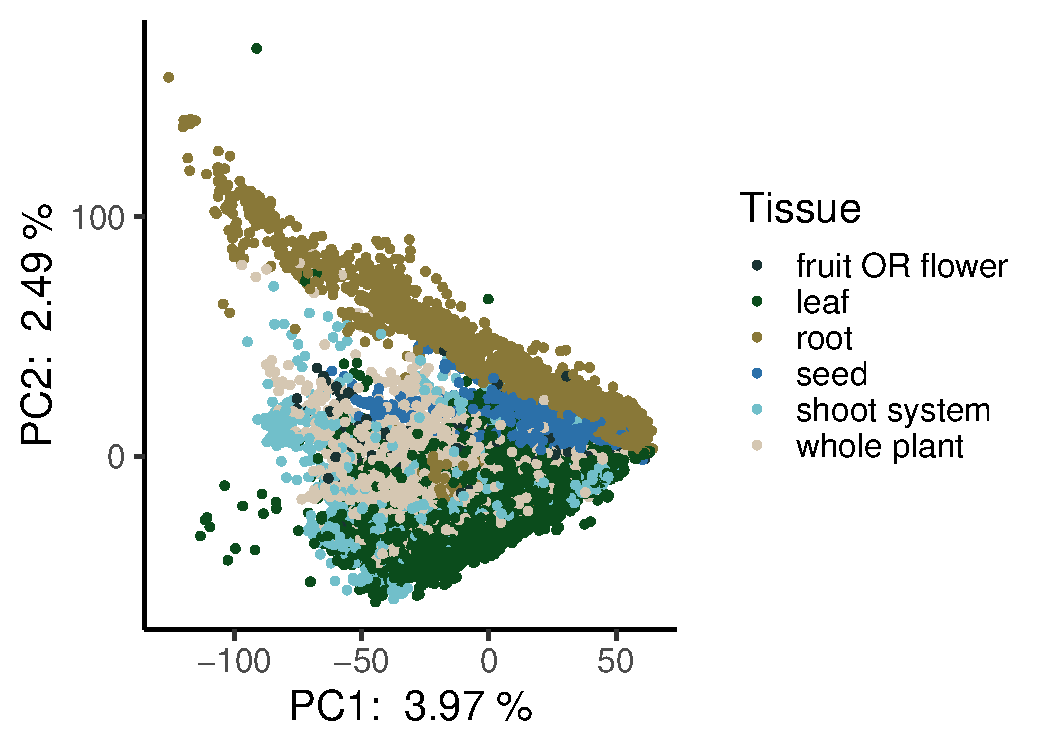
\includegraphics[width=\textwidth]{figures/chapter_1/pcaBySample_Tissue.pdf}
\caption{\textbf{Principal components analysis of all expression data.} Each point represents a different RNA-seq experiment and is colored by its associated tissue type. Experiments from all treatment conditions are included in this analysis. Plotting order was randomized to avoid overplotting.}%
\label{fig:pcaTissue}
\end{figure}

\begin{figure}[H]
\centering
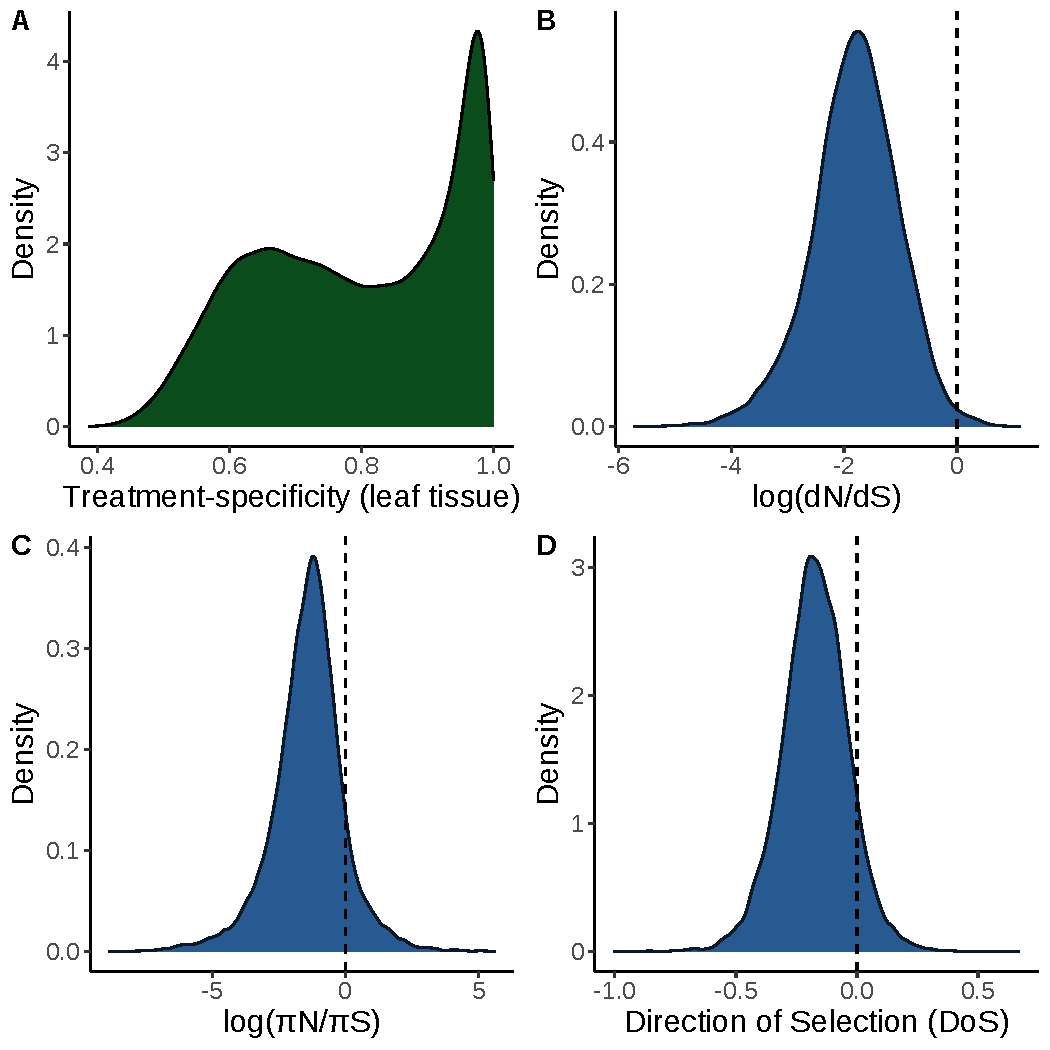
\includegraphics[width=\textwidth]{figures/chapter_1/histogramsOfKeyVariables.pdf}
\caption{\textbf{Density plots of key variables measured in this study.} (\textbf{A}) Distribution of treatment specificity in leaf tissue expression across all genes included in this study. The area underneath the curve in a given interval of treatment specificity represents the proportion of genes in this study that fall within that range of treatment specificity. (\textbf{B}) Distribution of $dN/dS$ across all genes included in this study. The area to the right of the dashed line represents the proportion of genes in this study with $dN/dS > 1$. (\textbf{C}) Distribution of $\pi_N/\pi_S$ across all genes included in this study. The area to the right of the dashed line represents the proportion of genes in this study with $\pi_N/\pi_S > 1$. (\textbf{D}) Distribution of DoS across all genes in this study. Area to the right of the dashed line represents the propotion of genes with DoS > 0, which is interpreted as evidence of adaptive evolution.}%
\label{fig:histKeyVariables}
\end{figure}

\subsubsection*{Omitting samples with low expression disentangles expression level and specificity}

\begin{double}

Genes that are only expressed in one treatment or tissue will, by definition, have low mean expression across all environments or tissues \citep{wright_effects_2004}. Thus, we sought a method of calculating expression level that was independent of treatment specificity. To better understand the relationship between average expression and treatment specificity, we calculated correlations between treatment-specificity and expression level while either including or excluding low expression values (TPM < 5) on our real RNA-seq dataset. We found that excluding low expression values decreased the correlation between average expression and treatment-specificity in leaf tissue samples (Figure \ref{fig:simulation}) and other tissues (Figures A34 - A38) and replicated the result by simulating gene expression matrices (Figure A39). Thus, for all later partial correlation analyses (see next section) we quantified each gene's average expression after dropping experiments where the gene was not expressed (TPM < 5).

\end{double}

\begin{figure}[H]
\centering
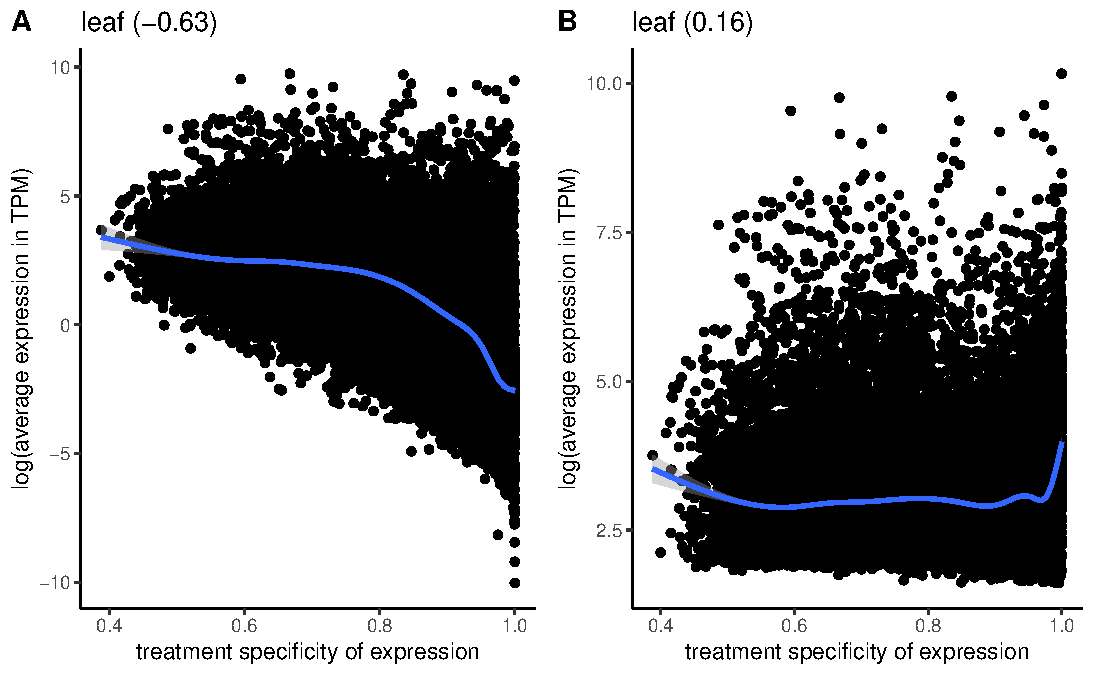
\includegraphics[width=\textwidth]{figures/chapter_1/leaf_treatmentSpecificityVsAverageExpression_withVsWithoutZeros.pdf}
\caption{\textbf{Correlation between the average expression in transcripts per million (TPM) and treatment specificity of genes.} Figures show correlations when samples with low expression ($< 5$ TPM) are included (\textbf{A}) vs excluded (\textbf{B}). Expression level and treatment specificity were calculated using only data from leaf tissue samples. Line is a smoothing line with 95 \% confidence intervals and values in parentheses give spearman correlation.}%
\label{fig:simulation}
\end{figure}

\subsubsection*{Treatment specificity correlates with levels of nonsynonymous diversity and divergence in genes}

\begin{double}
    
We next calculated partial correlations between treatment specificity and measures of selection after controlling for average expression, gene length, GC content, and tissue specificity in expression. These partial correlations were calculated separately for expression data on each tissue type and did not account for batch effects (see next section). Among leaf tissue samples, average expression had significant partial correlations with $dN$ ($\rho = -0.19$, p-value = $2.1\times10^{-122}$) and $\pi_N$ ($\rho = -0.17$, p-value = $2.8\times10^{-175}$) after controlling for other factors (Figures \ref{fig:pcorImbalanced}A,\ref{fig:pcorImbalanced}B). Treatment specificity was more strongly correlated with $dN$ ($\rho = 0.10$, p-value = $7.6\times10^{-31}$) and $\pi_N$ ($\rho = 0.10$, p-value = $1.2\times10^{-62}$) than Tajima's D ($\rho = 0.01$, p-value = $3.1\times10^{-7}$) and DoS ($\rho = 0.04$, p-value = $2.3\times10^{-06}$, Figure \ref{fig:pcorImbalanced}C, \ref{fig:pcorImbalanced}D). Furthermore, the top 25\% most treatment-specific genes in leaf tissue for our dataset have average $dN$ and $\pi_N$ values nearly 2.5 times greater than the 25\% least treatment-specific genes ($dN$ = 0.025 vs 0.061; $\pi_N$ = 0.0014 vs 0.0032). Meanwhile, the most and least treatment-specific genes have average Tajima's D values of are -0.44 and -0.43, respectively, and average $DoS$ values of -0.19 and -0.14, respectively. The strongest partial correlation generally occurred between tissue specificity and treatment specificity (Spearman's $\rho = 0.53-0.60$, Figure \ref{fig:pcorImbalanced}). Gene family size had among the weakest partial correlations with $\pi_{N}$ compared to other covariates, but strongly correlated with treatment specificity ($\rho = 0.12$, p-value = $6.3\times10^{-84}$, Figure \ref{fig:pcorImbalanced}B). All of these findings generally held when average expression and treatment specificity were calculated on data from other tissues (Table S2, Figures A6-A10).

\end{double}

\begin{figure}[H]
\centering
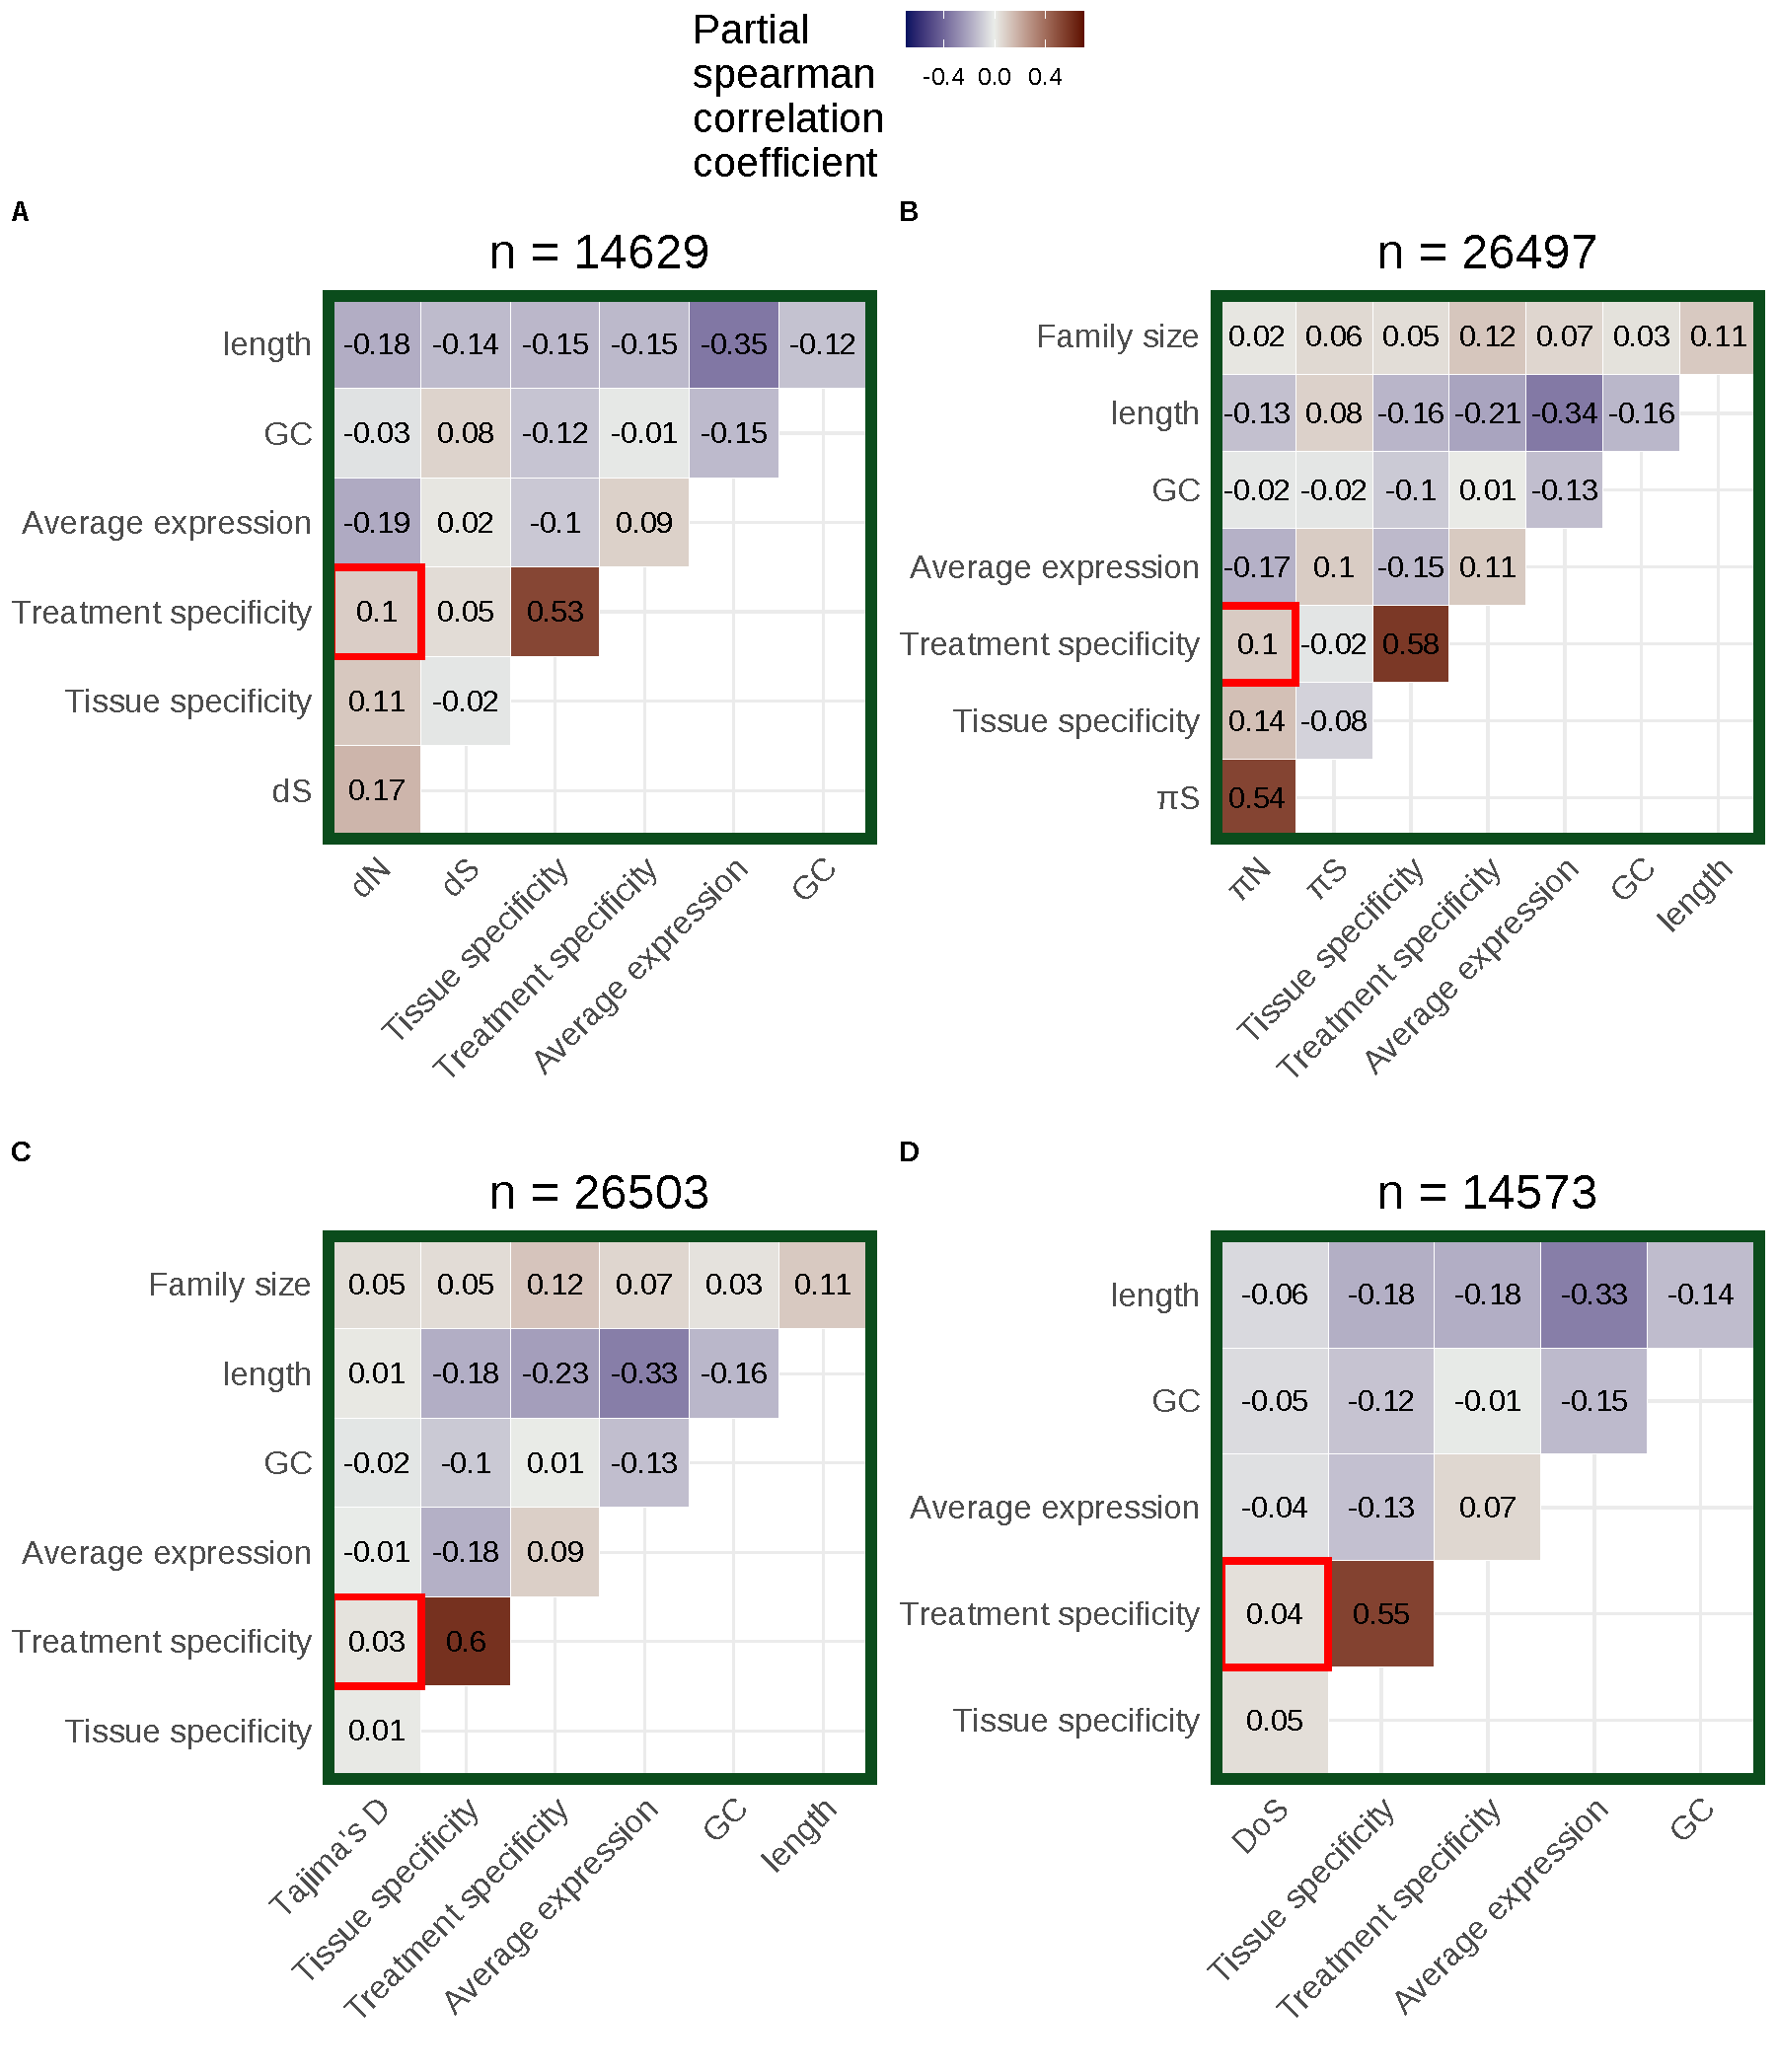
\includegraphics[width=\linewidth, height = \textheight, keepaspectratio]{figures/chapter_1/partialCorrelations_withTissueSpecificity_leaf_2023-02-20.pdf}
\caption{\textbf{Partial correlation analysis between specificity and selection.} Analyses include either (\textbf{A}) $dN$, (\textbf{B}) $\pi_N$, (\textbf{C}) Tajima's D, or (\textbf{D}) direction of selection (DoS) as a covariate. Average expression excludes values < 5 TPM and was calculated using only leaf tissue samples. Treatment specificity was also calculated using only leaf tissue samples. Tissue specificity was calculated using only control samples across all tissue categories. The number of genes included in each partial correlation analysis (n) is listed at the top of each heatmap.}%
\label{fig:pcorImbalanced}
\end{figure}

\subsubsection*{Correlations between treatment specificity and nonsynonymous variation persist after controlling for batch effects and dataset imbalance}

\begin{double}
    
While combining gene expression data across multiple studies can increase the statistical power of an analysis, there are some potential concerns. First, if many tissue-treatment combinations are not sampled, the dataset will be unbalanced and the effects of tissue and treatment variation on expression could be confounded. Consistent with this expectation, there was a high correlation between tissue specificity and treatment specificity in our initial analyses (Figure \ref{fig:pcorImbalanced}, S6-S10). Furthermore, combining data from multiple laboratories could generate batch effects \citep{leek_tackling_2010}. To address the issues of imbalance and batch effects, we first subset our data to only include treatments where all tissue types were represented. This subset included the treatments of control, abscisic acid, continuous light, warm/hot air temperature, and cold air temperature. We then used SVA to correct for the influence of unknown batch effects on this data subset \citep{leek_capturing_2007}. After SVA, treatment specificity positively correlated with $dN$ ($\rho = 0.10$, p-value = $1.6\times10^{-32}$) and $\pi_N$ ($\rho = 0.07$, p-value = $1.5\times10^{-23}$) when average expression and treatment specificity were calculated on combined fruit and flower data (Figures A33). However, treatment specificity in other tissue types generally did not correlate with our measures of selection (Figures A28-S33, Table S4).

The inclusion of only five treatments in the above analysis could limit quantification of a gene's treatment specificity. Thus, in order to include data from a larger number of treatments, avoid dataset imbalance, and avoid batch effects, we split our expression matrix into six subsets by tissue category. We then further removed treatments that only had expression data from one study to avoid confounding treatment effects with study-specific batch effects. We applied SVA \citep{leek_capturing_2007} to each of these tissue-specific subsets. After SVA, the expression profiles of most genes appear less treatment-specific (Figures A16-A21 panels A vs B). We also observed less separation in PCA space within treatment groups after SVA (for example, see Figures A16C and A16D). Average expression levels before SVA were generally correlated with expression levels after SVA (Figures A16-A21 panels A and B). In partial correlations on each SVA-corrected subset, treatment specificity significantly correlated with $dN$ ($\rho = 0.13$, p-value = $6.9\times10^{-50}$) and $\pi_N$ ($\rho = 0.16$, p-value = $3.9\times10^{-128}$) but less strongly correlated with Tajima's D ($\rho = 0.04$, p-value = $6.6\times10^{-10}$) and DoS ($\rho = 0.05$, p-value = $2.0\times10^{-8}$) for the leaf tissue data subset (Table 1, Figures \ref{fig:pcorTissueSubsetsAfterSVA}). These patterns were similar in other tissue types (Figures A11-A15, Table S3).

\end{double}

\begin{table}[H]
 \centering
 \begin{tabularx}{\textwidth}{|L|L|L|L|}
\hline
{\bf Pre/post-SVA} & {\bf Selection measure} & {\bf Partial correlation: selection vs treatment-specificity} & {\bf p-value}\\
\hline
Pre & $dN$ & 0.10 & $7.6\times10^{-31}$ \\
Post & $dN$ & 0.13 & $6.9\times10^{-50}$ \\
\hline
Pre & $\pi_N$ & 0.10 & $1.2\times10^{-62}$ \\
Post & $\pi_N$ & 0.16 & $3.9\times10^{-128}$ \\
\hline
Pre & Tajima's D & 0.03 & $3.1\times10^{-7}$ \\
Post & Tajima's D & 0.04 & $6.6\times10^{-10}$ \\
\hline
Pre & DoS & 0.04 & $2.3\times10^{-6}$ \\
Post & DoS & 0.05 & $2.0\times10^{-8}$ \\
\hline
\end{tabularx}
\caption{\textbf{Partial correlations between treatment-specificity and different measures of selection pre-SVA and post-SVA.} All correlation coefficients are spearman coefficients and are calculated only on leaf tissue samples. All p-values represent whether correlation coefficient significantly differs from 0.}
\end{table}

\begin{figure}[H]
\centering
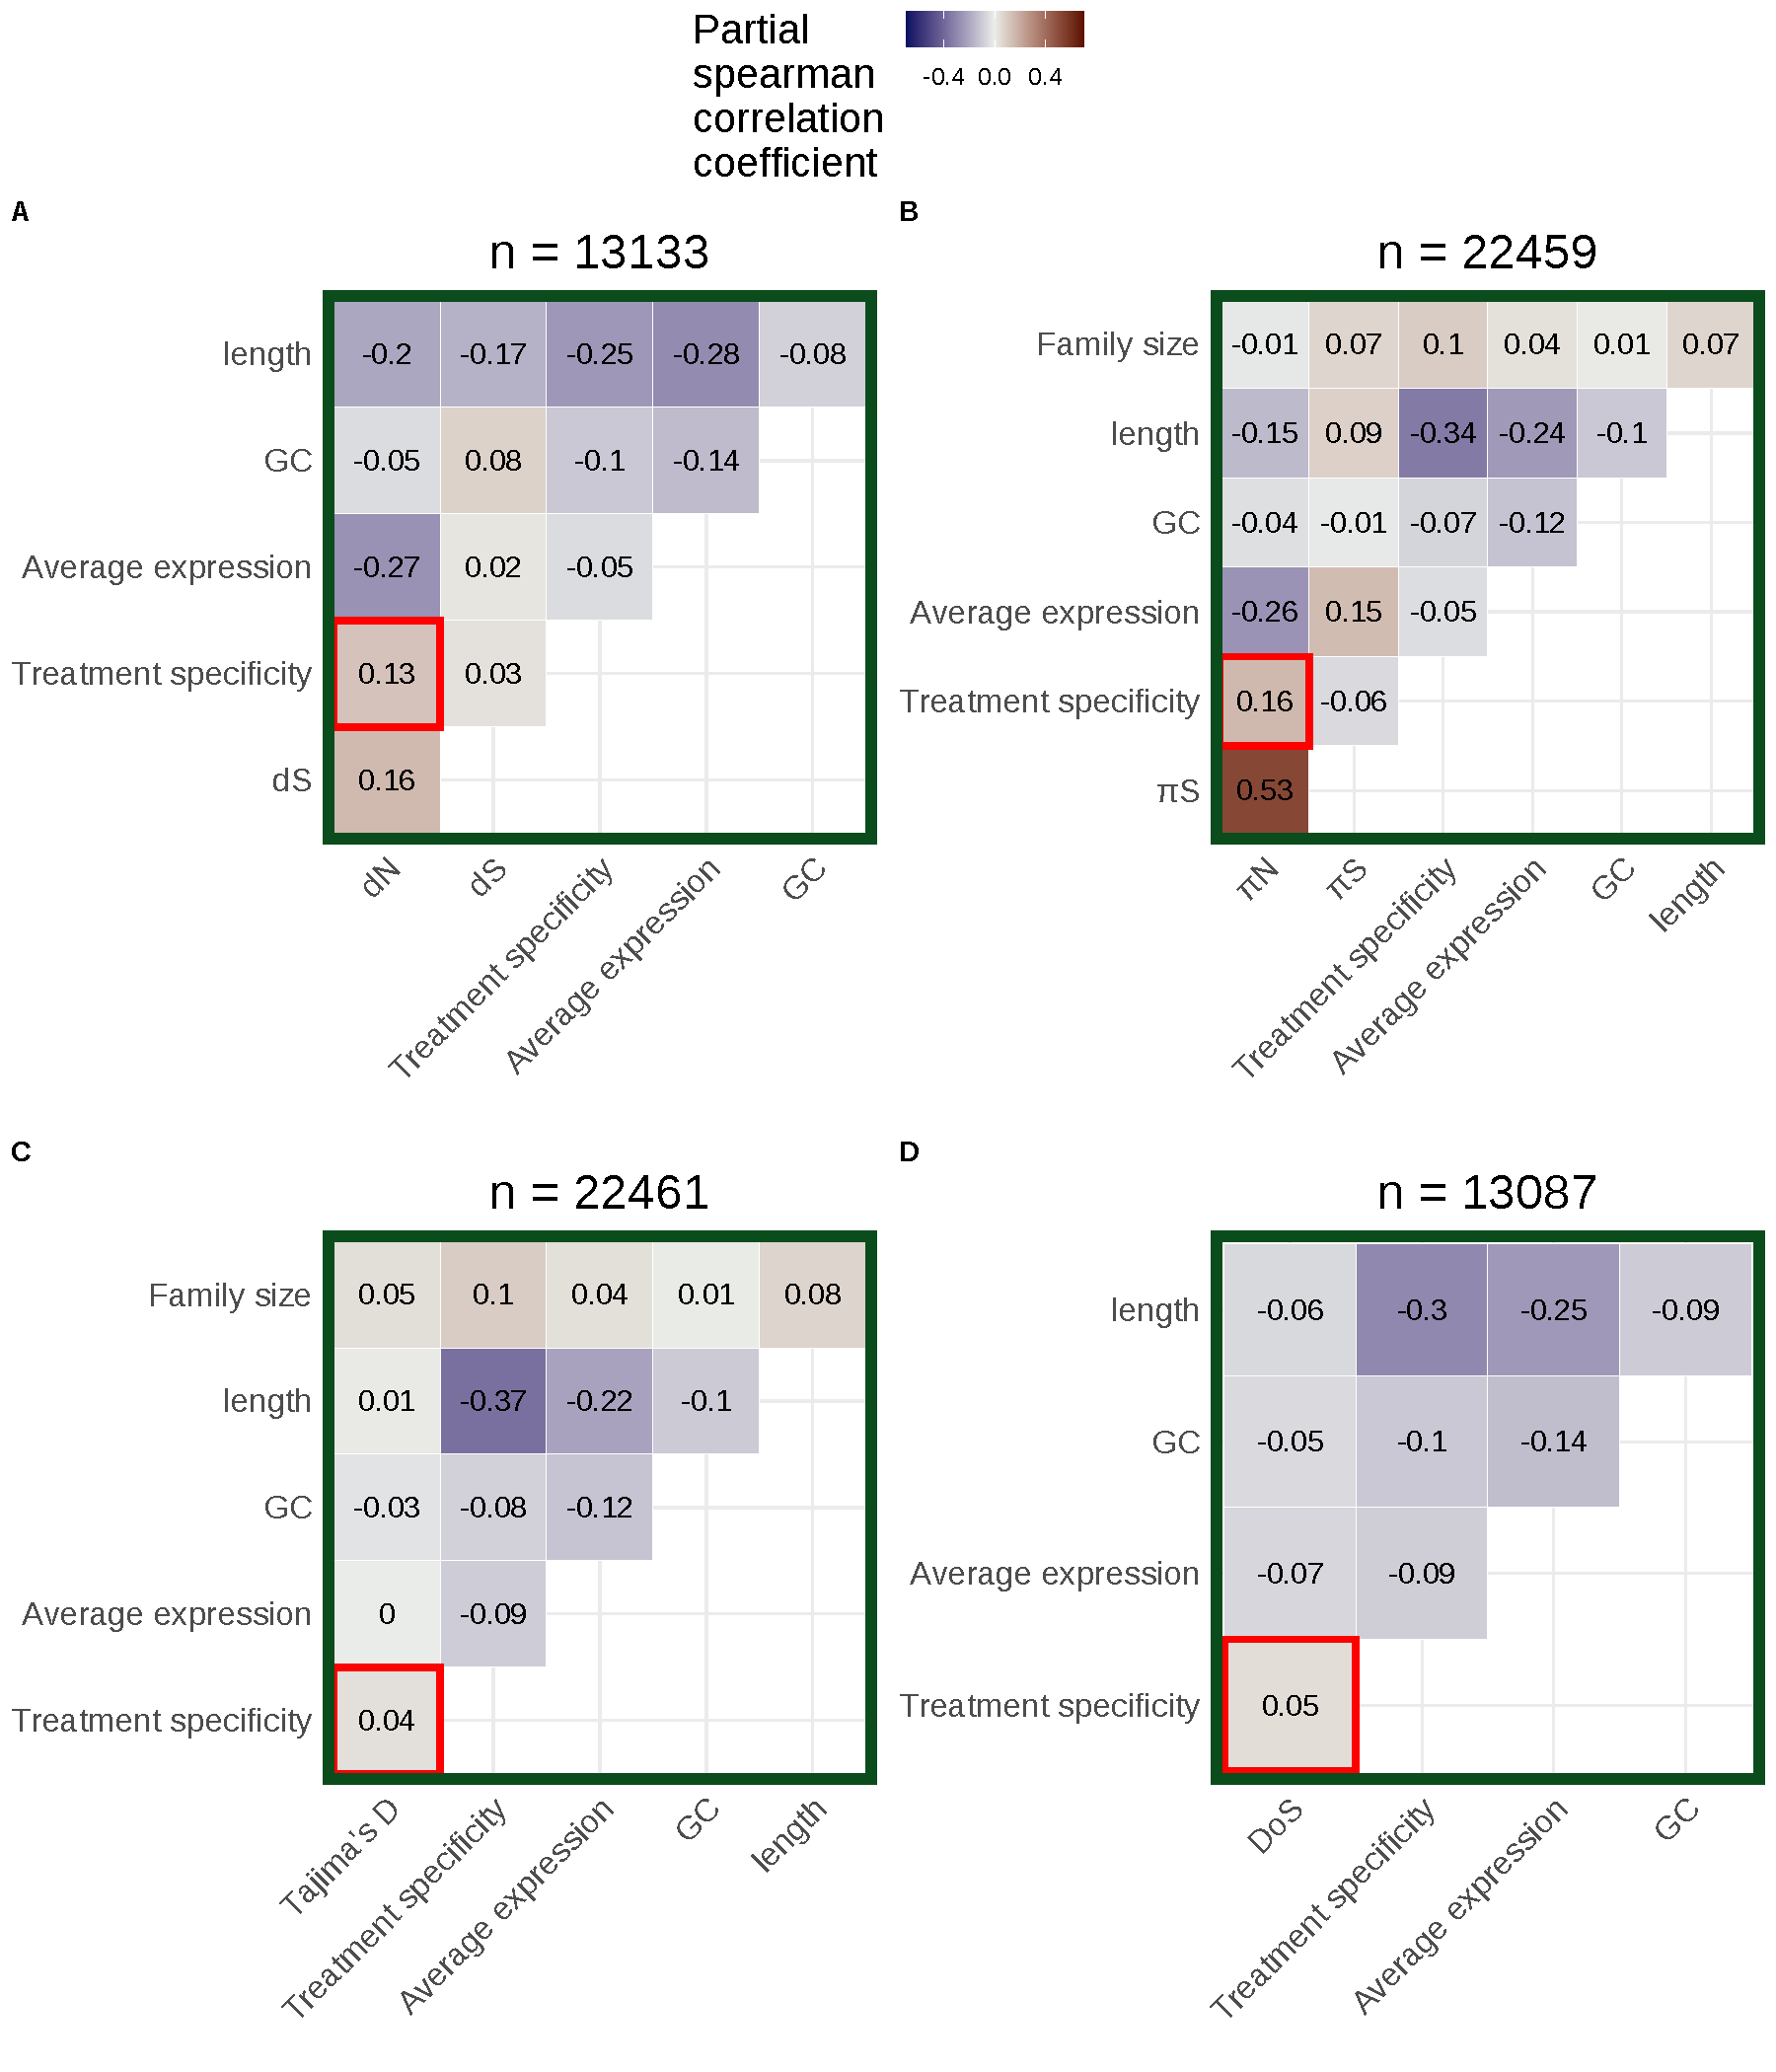
\includegraphics[width=\linewidth]{figures/chapter_1/partialCorrelations_withoutTissueSpecificityAfterSVA_leaf_2023-02-21.pdf}
\caption{\textbf{Partial correlations between specificity and selection after SVA.} Analyses include (\textbf{A}) $dN$, (\textbf{B}) $\pi_N$, (\textbf{C}) Tajima's D, and (\textbf{D}) direction of selection (DoS) based on leaf tissue data subset after applying SVA. Data was further subset to include only treatment groups with data from more than one study before applying SVA. Average expression calculation excludes values < 5 TPM. The number of genes included in each partial correlation analysis (n) is listed at the top of each heatmap.}%
\label{fig:pcorTissueSubsetsAfterSVA}
\end{figure}

\begin{double}

\subsection*{Discussion}
%\addcontentsline{toc}{subsubsection}{1.4: Discussion}
    
Our main finding is that genes with more treatment-specific expression patterns are, on average, under weaker selective constraint in \textit{A. thaliana}. This is evident by treatment-specific genes generally having higher values of $\pi_N$ and $dN$, but not higher values of Tajima's D and DoS, compared to genes with more constitutive expression (Figures \ref{fig:pcorImbalanced},\ref{fig:pcorTissueSubsetsAfterSVA}). Our result does not refute the possibility of strong positive selection on treatment-specific genes, as is the case for nucleotide binding site leucine rich repeat proteins (NBS-LRRs) in \textit{A. thaliana} \citep{mondragon-palomino_patterns_2002}. Rather, treatment-specific genes are simply under weaker selection on average compared to less treatment-specific genes. Altogether, this pattern is consistent with the hypothesis that a trade-off between the strength of selection and the treatment specificity of expression helps maintain variation in plasticity for \textit{A. thaliana} \citep{snell-rood_toward_2010, van_dyken_genetic_2010}.

There are a few ways to think about the biological relevance of the correlations of treatment specificity with $\pi_N$ and $dN$. First, the magnitude of treatment specificity's correlation with $\pi_N$ and $dN$ was generally half the magnitude of average expression's correlation with $\pi_N$ and $dN$ and similar to tissue specificity's correlation with $\pi_N$ and $dN$. Both tissue specificity and average expression are thought to be important determinants of protein evolution \citep{bush_lineage-specific_2015,wu_expression_2022}, suggesting the comparable effects of treatment specificity may be important too. Second, the effect of treatment specificity on $\pi_N$ and $dN$ persisted even after simultaneously controlling for expression level, tissue specificity, gene length, GC content, and batch effects. Finally, the top 25\% most treatment-specific genes in our dataset have average $dN$ and $\pi_N$ values nearly 2.5 times greater than the 25\% least treatment-specific genes ($dN$ = 0.025 vs 0.061; $\pi_N$ = 0.0014 vs 0.0032), but relatively similar Tajima's D and DoS values (Tajima's D = -0.44 vs -0.43; DoS = -0.19 vs -0.14). These observations together suggest that treatment specificity is an important determinant of protein evolution.

This study disentangles several processes that were often difficult to resolve in previous research. First, many previous studies focus mainly on explaining trends in $dN/dS$ \citep{slotte_genomic_2011, gaut_patterns_2011, bush_lineage-specific_2015}, but both relaxed negative selection and increased positive selection can lead to increases in $dN/dS$. To tease apart these two processes, we additionally investigated treatment specificity's relationship with Tajima's D and DoS. Treatment specificity's weaker correlation with Tajima's D and DoS, compared to $dN$ and $\pi_N$, suggests that relaxed negative selection plays a larger role than increased positive selection in explaining the high evolutionary rates of treatment-specific genes. Furthermore, measures of expression specificity are often highly correlated with expression level \citep{slotte_genomic_2011, alvarez-ponce_evolutionary_2012, Huang_dissecting_2022}. When calculating a gene's expression level, we only included samples where said gene was expressed (TPM > 5) to get an estimate of expression level that was still correlated with $dN$ and $\pi_N$, but was independent of expression specificity, allowing us to better disentangle these factors. Finally, previous studies have struggled to partition the factors that influence selection on genes in the presence of predictor variables with considerable error, such as expression level \citep{drummond_single_2006, plotkin_assessing_2007, yang_factors_2011}. Error in expression measurements can often be attributed to unmeasured differences between RNA-sequencing experiments \citep{leek_tackling_2010} and we accounted for these differences using SVA \citep{leek_capturing_2007}. Even after SVA, treatment specificity was strongly correlated with $dN$ and $\pi_N$ (Figures \ref{fig:pcorTissueSubsetsAfterSVA}A-B), suggesting our results are not an artifact of errors in expression measurement or combining expression data across many studies. 

Surprisingly, nearly all genes in \textit{A. thaliana} have some degree of treatment specificity in their expression (Figures \ref{fig:histKeyVariables}A, A3), reflecting results of previous studies on tissue specificity \citep{eisenberg_human_2003}. The high prevalence of treatment specificity in our dataset is partly explained by batch effects because SVA significantly lowered the apparent treatment specificity of most genes (Figures A16B-A21B) and reduced within-treatment differentiation in PCA space (for example, see Figures A16C and A16D). This reduction in treatment-specificity likely happened because batch effects can include unrecorded between-treatment differences (e.g. the humidity of the growth chamber, light intensity, watering schedule, etc.). Controlling for these unrecorded between-treatment differences thus causes the expression of genes to be less treatment-specific. However, even after batch correction most genes still showed some degree of treatment specificity (Figures A16B-A21B), suggesting it is rare for a gene to be expressed at the same level across many environments.

We also observed that genes with higher treatment specificity generally belonged to larger gene families. We expected gene family size to correlate with selection because singleton and duplicated genes often evolve at different rates \citep{jordan_duplicated_2004, davis_preferential_2004}. Theory also suggests that gene duplication leads to relaxation of selection on duplicates, allowing for neo- and sub-functionalization \citep{lynch_evolutionary_2000, aagaard_relaxed_2006}. We could not investigate how gene family size correlates with $dN$ or DoS because measuring these quantities requires identifying substitutions between orthologous genes. Thus, $dN$ and $DoS$ can only be reliably measured for 1:1 orthologs between \textit{A. thaliana} and \textit{A. lyrata}. However, $\pi_N$ and Tajima's D can be calculated for genes in larger families and we did observe persistent correlations between family size and Tajima's D (For Figure \ref{fig:pcorTissueSubsetsAfterSVA}C: $\rho = 0.05$, p-value = $3.1\times10^{-12}$; also see Figures A6C-A15C, A28C-A33C). Altogether, these correlations suggest that processes of gene duplication, neofunctionalization, and subfunctionalization could be connected to evolving some degree of treatment specificity.

Gene length was generally the second most correlated factor with $dN$ and $\pi_N$ in our study, just behind average expression. This is consistent with previous work suggesting that longer proteins require more energy to synthesize and are thus under stronger selective constraints \citep{urrutia_codon_2001, castillo-davis_selection_2002, eisenberg_human_2003, urrutia_signature_2003}. However, while some previous studies in \textit{A. thaliana} observe this same trend \citep{bush_lineage-specific_2015}, others do not \citep{slotte_genomic_2011}. This discrepancy could be due to differences in how gene length is defined between studies. In this study, each gene's length included coding sequence as well as introns and untranslated regions, whereas other studies break down gene length into individual features \citep{bush_lineage-specific_2015}. The goal of this study was not to understand differences in evolution between different gene features, so we included all gene features in our estimate of gene length. However, introns and untranslated regions experience different evolutionary patterns than coding sequences; for example, highly expressed genes being under selection for shorter introns \citep{castillo-davis_selection_2002, eisenberg_human_2003}. Therefore, future studies must clearly define even seemingly simple features like gene length to ensure that results are comparable across studies. 

Although we focused on testing the idea that treatment specificity is responsible for relaxed negative selection in some genes, it is also possible that relaxed selection caused the evolution of treatment specificity. There is some evidence that relaxation of selection occurs before the evolution of expression specificity \citep{hunt_relaxed_2011} and may better explain cases of neo- and subfunctionalization \citep{lynch_evolutionary_2000, aagaard_relaxed_2006}. Future experiments that look at the evolution of treatment specificity and sequence evolution across a broader phylogenetic scale may be helpful for determining the order of these processes.

In summary, this study investigates a trade-off between the treatment-specific expression of a gene and the strength of selection said gene experiences, which is hypothesized to limit plasticity evolution. Consistent with this hypothesis, genes in \textit{A. thaliana} with more treatment-specific expression are under weaker selection compared to more evenly expressed genes. While we find that this trade-off exists, we could not dissect the direction of causality in the trade-off or determine how much this trade-off constrains plasticity evolution relative to other processes. However, these are exciting areas of future research. Future studies should ideally generate fully balanced datasets on gene expression acquired across natural environmental gradients. Taking these steps will contribute to a comprehensive understanding of the constraints on plasticity and protein evolution.

\vspace{4pt}

\subsection*{Data availability}
    
Supplemental figures are available in Appendix A. All code for our bioinformatic workflows, data analysis, and figure creation can be found here: \href{https://github.com/milesroberts-123/arabidopsis-conditional-expression}{https://github.com/milesroberts-123/arabidopsis-conditional\hyp{}expression}. All supplementary tables are available online at: \url{https://doi.org/10.1093/genetics/iyad074}. The tissue type and treatment annotations for RNA-seq runs in our study can be found in Table S5. Genomic references, mapping rates, and a table of expression specificity; nucleotide diversity; and substitution rate values estimated for all \textit{A. thaliana} genes included in this manuscript's analyses is available at: \url{https://doi.org/10.5061/dryad.xd2547dnd}. The genome assembly and annotation used in this study was originally downloaded from Phytozome: \url{https://phytozome-next.jgi.doe.gov/}.

\end{double}

\newpage

\section*{CHAPTER 2: $k$-MER-BASED DIVERSITY SCALES WITH POPULATION SIZE PROXIES MORE THAN NUCLEOTIDE DIVERSITY IN A META-ANALYSIS OF 98 PLANT SPECIES\footnote{This chapter is, as of writing, accepted for publication at \textit{Evolution Letters}. The preprint version is currently available at the following DOI under a CC-BY License: https://doi.org/10.1101/2024.05.17.594778}}
\addcontentsline{toc}{subsection}{{CHAPTER 2: \textit{k}-MER-BASED DIVERSITY SCALES WITH POPULATION SIZE PROXIES MORE THAN NUCLEOTIDE DIVERSITY IN A META-ANALYSIS OF 98 PLANT SPECIES}}

\setcounter{figure}{0}
\renewcommand{\figurename}{Figure}
\renewcommand{\thefigure}{2.\arabic{figure}}

\setcounter{equation}{0}
\renewcommand{\theequation}{2.\arabic{equation}}

\begin{double}

\vspace{4pt}

\subsection*{Abstract}

A key prediction of neutral theory is that the level of genetic diversity in a population should scale with population size. However, as was noted by Richard Lewontin in 1974 and reaffirmed by later studies, the slope of the population size-diversity relationship in nature is much weaker than expected under neutral theory. We hypothesize that one contributor to this paradox is that current methods relying on single nucleotide polymorphisms (SNPs) called from aligning short reads to a reference genome underestimate levels of genetic diversity in many species. As a first step to testing this idea, we calculated nucleotide diversity ($\pi$) and $k$-mer-based metrics of genetic diversity across 112 plant species, amounting to over 205 terabases of DNA sequencing data from 27,488 individuals. After excluding 14 species with low coverage or no variant sites called, we compared how different diversity metrics correlated with proxies of population size that account for both range size and population density variation across species. We found that our population size proxies scaled anywhere from about 3 to over 20 times faster with $k$-mer diversity than nucleotide diversity after adjusting for evolutionary history, mating system, life cycle habit, cultivation status, and invasiveness. The relationship between $k$-mer diversity and population size proxies also remains significant after correcting for genome size, whereas the analogous relationship for nucleotide diversity does not. These results are consistent with the possibility that variation not captured by common SNP-based analyses explains part of Lewontin's paradox in plants, but larger scale pangenomic studies are needed to definitively address this question.  

\vspace{4pt}

\subsection*{Introduction}
%\addcontentsline{toc}{subsubsection}{2.1: Introduction}
    
Understanding the determinants of genetic diversity within populations is key to informing species conservation \citep{cole_genetic_2003} and breeding efforts \citep{sanchez_improving_2023}. However, most species have far less genetic diversity (commonly estimated as pairwise nucleotide diversity, $\pi$) than expected \citep{frankham_how_2012, corbett-detig_natural_2015, buffalo_quantifying_2021}. If we assume that the vast majority of genetic variants are neutral, then the determinants of genetic diversity are encapsulated in neutral theory \citep{kimura_neutral_1983}: $E[\pi] \approx 4N_e\mu$, where $E[\pi]$ is the expected level of genetic diversity, $N_e$ is the effective size of a population, and $\mu$ is the mutation rate per base pair per generation. Mutations rates for SNPs and small indels vary relatively little across species \citep{cagan_somatic_2022, bergeron_evolution_2023, quiroz_causes_2023}, while the total number of individuals in a species varies massively \citep{buffalo_quantifying_2021}. Thus, under neutral theory, population size should be a strong determinant of genetic diversity and species with larger population sizes should be more diverse. However, even some of the most abundant species studied to date have low genetic diversity compared to neutral theory expectations. For example, \textit{Drosophila simulans} has an estimated population size $>10^{14}$ and a diversity of $\pi \approx 0.01$, but an expected diversity of $\pi > 0.1$  \citep{buffalo_quantifying_2021}.  This mismatch between expected and observed levels of neutral diversity across populations of varying size is known as Lewontin's paradox, named after Richard Lewontin who first described the phenomenon \citep{lewontin_genetic_1974}. 

The potential mechanisms underlying Lewontin's paradox have been reviewed extensively \citep{leffler_revisiting_2012, slotte_impact_2014, ellegren_determinants_2016, charlesworth_how_2022}. Multiple selective and demographic processes likely contribute to Lewontin's paradox; however, determining the relative importance of these processes remains a contentious area of research. The two most explored mechanisms are historic population size changes (i.e. demography, \citet{charlesworth_how_2022}) and linked selection - whereby fixation or purging of selected alleles causes the loss of linked neutral alleles \citep{kojima_accumulation_1964, kojima_survival_1967, smith_hitch-hiking_1974, charlesworth_effect_1993, charlesworth_effect_1994}. Linked selection is expected to reduce diversity more in regions of lower recombination and higher functional density \citep{slotte_impact_2014} and many studies have tested this hypothesis\citep{tenaillon_patterns_2001, hellmann_neutral_2003, nordborg_pattern_2005, roselius_relationship_2005, branca_whole-genome_2011, paape_fine-scale_2012, corbett-detig_natural_2015, silva-junior_genome-wide_2015, wang_natural_2016, phung_determining_2016, mackintosh_determinants_2019}. These previous investigations often conclude that linked selection contributes to Lewontin's paradox, but not all report significant results (e.g. \citet{schmid_multilocus_2005, roselius_relationship_2005, flowers_natural_2012, wang_natural_2016}). It's been argued that studies focused on plant species especially tend to find weaker evidence for linked selection \citep{slotte_impact_2014}. There is also both empirical and theoretical evidence that linked selection is unlikely to explain the entirety of Lewontin's paradox, suggesting that demographic factors play an important role too \citep{coop_does_2016, buffalo_quantifying_2021, charlesworth_how_2022}. 

There are three main types of demographic changes proposed to contribute to Lewontin's paradox: contractions, expansions, and cyclical population size changes \citep{charlesworth_how_2022}. Population contractions cause loss of diversity. Thus, if many species' populations recently contracted (due to human activity, for example), then their contemporary diversity would be much lower than expected from their pre-contraction population sizes \citep{exposito-alonso_genetic_2022}. Recent population expansions could cause a similar mismatch. Because it takes many generations for populations to accumulate diversity compared to the timescale of typical expansions, contemporary diversity levels for an expanded population would be much smaller than expected from a post-expansion population size \citep{peart_determinants_2020, charlesworth_how_2022}. For a similar reason, species that have seasonal variation in their population sizes will also tend to have diversity levels closer to what one would expect based on their minimum size rather than their peak size \citep{wright_breeding_1940}. Studies investigating Lewontin's paradox would ideally try to jointly infer these demographic histories alongside selective factors in natural populations. However, issues of model complexity and identifiability often prevent such joint estimation \citep{johri_toward_2020, johri_prospect_2022, johri_recommendations_2022}, suggesting further explorations of Lewontin's paradox will require new approaches.

Two potential, but rarely explored, contributors to Lewontin's paradox are that (1) current methods for estimating genetic diversity systematically underestimate the true levels of genetic diversity in most populations and (2) changes or corrections to the calculation of diversity could yield stronger correlations with population size. Lewontin's original observations and earlier studies on the population size-diversity relationship were based on allozymes, which detect variants in protein sequences \citep{lewontin_genetic_1974, nei_extent_1984}. More recent studies  measure diversity using SNPs at more neutral four-fold degenerate sites (i.e. sites where mutations do not affect protein sequences) in DNA and generally observe greater within-species diversity and between-species divergence compared to allozymes \citep{li_low_1991, makalowski_evolutionary_1998, bazin_population_2006, piganeau_evidence_2009}. However, current SNP-based methods are not perfect either and there is significant evidence that SNPs capture a biased and incomplete picture of genetic diversity. Calling SNPs typically requires aligning reads to a reference genome, meaning any SNPs in regions that are not present or highly diverged from the reference genome will be excluded from analysis and thus downwardly bias diversity estimates \citep{golicz_pangenomics_2020, buffalo_quantifying_2021}. This downward bias is typically assumed to have little effect on the qualitative relationship between diversity and $N_e$ \citep{buffalo_quantifying_2021}, but recent pangenomic studies have uncovered troves of non-reference variation across a variety of species (\citet{ebler_pangenome-based_2022, rice_pangenome_2023}, reviewed in \citet{Bayer_plant_2020}). Sometimes alignment errors in regions of non-reference structural variation will also create false positive SNP calls, which will also affect diversity estimates (e.g. \citet{jaegle_extensive_2023}). Finally, previous meta-analyses of population size and diversity data rely on scraping diversity estimates from previously published studies (\citet{frankham_how_2012, buffalo_quantifying_2021}, except see \citet{corbett-detig_natural_2015}). However, many studies report inaccurate SNP calls and deflated diversity estimates due to errors in the handling of missing genotype calls \citep{korunes_pixy_2021, schmidt_unbiased_2021, sopniewski_estimates_2024} and may filter genotype calls differently, making comparisons across species difficult. Overall, errors in diversity calculations and omission of diversity in genomic regions that are either difficult or impossible to align to could partially explain Lewontin's paradox. Re-analyzing whole genome sequencing data with a common pipeline and applying correct calculations of nucleotide diversity would make diversity estimates across species more comparable and easier to interpret \citep{buffalo_quantifying_2021, mirchandani_fast_2024}. 

One useful pangenomics tool for measuring non-reference variation that is readily applicable to common short-read datasets is the $k$-mer. $k$-mers are subsequences of length $k$ derived from a larger sequence and they have a long history of use in computer science \citep{shannon_mathematical_1948}, genome assembly \citep{turner_integrating_2018}, metagenomics \citep{benoit_multiple_2016}, and quantitative genetics \citep{rahman_association_2018, voichek_identifying_2020, kim_dissecting_2020, mehrab_efficient_2021}. Recent studies have also demonstrated the utility of $k$-mers for measuring heterozygosity and genetic differences between individuals (commonly referred to as ``dissimilarity" measures, \citet{ondov_mash_2016, vurture_genomescope_2017, ranallo-benavidez_genomescope_2020, vanwallendael_alignment-free_2022, roberts_k-mer-based_2024}). Typical analysis of $k$-mers involves only counting the presence/absence and/or frequencies of all $k$-mers in a set of reads, without aligning the reads to any reference, then deriving measures of genetic difference from such counts \citep{benoit_multiple_2016}. Avoiding alignment allows one to incorporate sequences that would otherwise be omitted for lack of alignment to a reference genome \citep{rahman_association_2018, voichek_identifying_2020, wiersma_k-mer_2024}.

We revisited Lewontin's paradox in plants using $k$-mer-based measures of genetic difference and corrected $\pi$ calculations, aiming to test whether the inclusion of non-reference variation or modifications to diversity calculations could increase the scaling between population size proxies and diversity. We compared how $k$-mer dissimilarity and typical SNP-based estimates of nucleotide diversity correlated with population size proxies across a large panel of plant species - all processed through the same bioinformatic pipeline. Our expectation was that if $k$-mers are better at capturing genomic variation than SNPs, $k$-mer dissimilarity would scale more rapidly with population size compared to nucleotide diversity.

\vspace{4pt}

\subsection*{Methods}
%\addcontentsline{toc}{subsubsection}{2.2: Methods}
    
Our entire analysis is packaged as a snakemake workflow stored here: \href{https://github.com/milesroberts-123/tajimasDacrossSpecies}{https://github.com/milesroberts-123/tajimasDacrossSpecies}. This workflow includes the code to reproduce all of the steps individually explained below, along with instructions on how to run the code, and yaml files describing the exact configurations of software we used at each step. It also includes an example directed acyclic graph showing the order of steps a typical sample is processed through. The code detailing all initial, exploratory, and confirmatory data analyses as well as figure creation can be found as an R-markdown file in the github repository. The parameters for each software were kept constant across all datasets (except occasionally for the ``--ploidy" parameter in GATK HaplotypeCaller) to ensure that variation in bioinformatic processing did not bias our results. All statistical analyses used R v4.2.2 \citep{r_core_team_r_2022} and all color palettes used in figure creation come from the scico R package \citep{pedersen_scico_2023} to ensure color-blind accessibility.

\vspace{4pt}

\subsubsection*{Population-level sequencing data collection}

We started by building a list of species with high quality, publicly available reference genomes as well as population-level sequencing data. The source for the genome assembly and annotation used for each species in this study is listed in Table S1. We first downloaded all genomes in Phytozome (\href{https://phytozome-next.jgi.doe.gov/}{https://phytozome-next.jgi.doe.gov/}) with unrestricted data usage. We then downloaded all genomes for species from Ensembl plants (\href{https://plants.ensembl.org/index.html}{https://plants.ensembl.org/index.html}) that were not already represented in Phytozome. Next, we downloaded genomes for additional species from the NCBI genome database (\href{https://www.ncbi.nlm.nih.gov/genome/}{https://www.ncbi.nlm.nih.gov/genome/}) that were not already present in either Phytozome or Ensembl and met all of the following criteria: 

\begin{myitemize}
    \item matched filters: eukaryotic, plants, land plants, and exclude partial
    \item included assemblies of nuclear DNA (i.e. not just plastid genomes)
    \item included annotations of coding sequences
\end{myitemize} 

We also downloaded a genome for \textit{Nicotiana tabaccum} from the Sol genomics network (\url{https://solgenomics.net/}). Finally, we omitted 8 species (\textit{Aegilops tauschii}, \textit{Hordeum vulgare}, \textit{Lens culinaris}, \textit{Pisum sativum}, \textit{Thinopyrum intermedium}, \textit{Trifolium pratense}, \textit{Triticum aestivum}, \textit{Triticum turgidum}) that had at least one chromosome longer than $2^{29}$ bp (about 537 Mb) from all downstream analyses because tabix indexing, which is often utilized for SNP-calling pipelines, does not support chromosomes exceeding this length. In the end, we were left with genome assemblies and annotations for 112 plant species (see Table S1).

Note that, similar to previous studies \citep{corbett-detig_natural_2015, buffalo_quantifying_2021}, many of the plant species in this set of 112 are domesticated (see Table S1). This means that many of the species in our dataset have likely undergone recent demographic changes. However correctly accounting for demography is a general limitation of Lewontin's paradox studies, as we can only estimate proxies of $N_e$ for contemporary populations \citep{corbett-detig_natural_2015, buffalo_quantifying_2021}. We include cultivation status in our downstream modeling to help account for systematic differences between cultivated and wild species (see \textbf{Statistical analysis}) and also repeat our analysis with multiple types of population size proxies.

For each species with a reference genome, we searched for DNA-seq runs in the National Center for Biotechnology Information's Sequence Read Archive (SRA) with a name in the organism field that matched the species name (e.g. search for Arabidopsis lyrata[Organism] to get \textit{Arabidopsis lyrata} runs). We downloaded the run info for each search and found the study with most sequenced individuals for inclusion in our analysis. Most datasets came from individual studies, with the exception of \textit{Zea mays}, which included several studies described in \citet{bukowski_construction_2017}. The datasets used for each species are listed in Table S1.

We limited the size of each species' dataset to no more than $7.5 \times 10^{12}$ bp and no more than 1200 individuals because this defined the amount of data our workflow could process without the peak memory limit exceeding 50 TB and the time limit for genotype calling exceeding 7 days. If a species' dataset exceeded either 1200 individuals or $7.5 \times 10^{12}$ bp, we randomly dropped one individual at a time until both of these limits were satisfied. 

We downloaded the SRA runs associated with each individual using the SRA toolkit (v2.10.7), then trimmed low-quality base calls with fastp (v0.23.1, \citet{chen_fastp_2018}), requiring a minimum quality score of 20 and a minimum read length of 30 base pairs. For each species, we summarized the results of fastp trimming using multiqc (v1.18, \citet{ewels_multiqc_2016}). After trimming, any fastq files that were technical replicates of the same individual were concatenated. Concatenated fastq files were then processed through two different workflows: SNP-calling and $k$-mer counting.

\vspace{4pt}

\subsubsection*{SNP calling pipeline}

We aligned sequencing reads for each individual to their respective reference genome using BWA MEM (v0.7.17, \citet{li_fast_2009, li_aligning_2013}), sorted the resulting BAM files with samtools (v1.11, \citet{danecek_twelve_2021}), and marked optical duplicates with picardtools (picard-slim v2.22.1, \citet{broad_institute_picard_2019}). Next, we called SNPs with GATK HaplotypeCaller (v4.1.4.1, \citet{mckenna_genome_2010, poplin_scaling_2018}). We varied the --ploidy parameter for HaplotypeCaller between species depending on the actual ploidy recorded in the literature and whether individual subgenome assemblies were available. However, the vast majority of species in our dataset had a --ploidy paramter of 2. We restricted genotype calling to only 4-fold degenerate sites within the nuclear genome and included all nuclear genome scaffolds, as identified by degenotate (v1.1.3, \citet{mirchandani_fast_2024}), to focus solely on neutral diversity. Notably, we chose to not call SNPs in non-coding sequences in plants because plant genomes tend to be highly repetitive and are largely composed of transposable elements, making short read mapping difficult For example, even in the small-genome plant species \textit{Capsella grandiflora}, SNPs can only be confidently called in 10\% of intergenic sites \citep{williamson_evidence_2014}. Runs for each species were then combined with GATK GenomicsDBImport, then genotyped with GATK GenotypeGVCFs, including invariant sites as done in \citet{korunes_pixy_2021}. Variant and invariant sites were separated with bcftools (v1.17, \citet{danecek_twelve_2021}) and then filtered separately, as recommended by \citet{korunes_pixy_2021}. Variant sites were removed from our analyses if they met at least one of the following criteria: number of alleles $>$ 2, indel status = TRUE, fraction of missing genotypes $>$ 0.2, QD $<$ 2.0, QUAL $<$ 30.0, MQ $<$ 40.00, FS $>$ 60.0, HaplotypeScore $>$ 13.0, MQRankSum $<$ -12.5, and ReadPosRankSum $<$ -8.0. In short, these filters reflect the standard population genetics practices of removing non-biallelic SNPs and SNPs with a lot of missing genotype calls. The exact filter cutoffs also come from GATK Best Practices for hard filtering \citep{caetano-anolles_hard-filtering_2023} that is widely used (e.g. \citep{yu_genome-wide_2024, ramirez-ramirez_comparing_2024, glasenapp_selection_2024, ritter_buds_2024}). For each species, we also required that each variant site have a minimum read depth of 5, but no more than 3 times the genome-wide average read depth at variant sites for that species. We chose a minimum read depth of 5 to maintain comparability with our $k$-mer dissimilarity calculations which required minimum $k$-mer counts of 5 (see \textbf{$k$-mer counting}), but we also filtered out calls with very high read depths because these could represent read mismapping due to repetitive or paralogous regions. Meanwhile, invariant sites were removed from our analyses if they met at least one of the following criteria: QUAL $>$ 100.0, read depth $\leq$ 5, or read depth $\geq$ 3 times the genome-wide average read depth at invariant sites for that species. Finally, invariant and variant sites were concatenated into a single VCF file per scaffold using bcftools. For \textit{Brassica napus} and \textit{Miscanthus sinensis}, scaffolds named ``LK032656" (195,249 bp, 0.023 \% of the genome) and ``scaffold04645" (2,838 bp, 0.000136 \% of the genome), respectively, were omitted from our analyses because an error in SLURM job cancellation caused snakemake to prematurely delete intermediate files for these scaffolds. It is worth noting that different choices of genotype callers and filtering parameters could lead to different estimates of nucleotide diversity. However, our workflow is representative of SNP calling workflows used in many published population genetic analyses. 

Using the SNP genotypes called from our pipeline, we then calculated genome-wide average nucleotide diversity at four-fold degenerate sites ($\bar{\pi}$) using the filtered set of variant and invariant sites. To do this, we first calculated heterozygosity at each four-fold degenerate site ($i$) according to \citet{hahn_molecular_2018}: 

\begin{equation}
\pi_i = \left( \frac{n_i}{n_i-1} \right) \left( 1 - \sum_{j = 1}^{a_i} p_{ij}^2 \right)
\end{equation}
where $n_i$ is the number of sequenced chromosomes with non-missing genotypes for site $i$, $a_i$ is the number of alleles for site $i$, and $p_{ij}$ is the frequency of the $j$th allele at site $i$. For each invariant site, the equation reduces to $\pi_i = 0$ because $p_{i1} = 1$ and $a_i = 1$. To get $\bar{\pi}$, we then calculated the average value of $\pi_i$ across all $M$ sites in the genome (including both variant and invariant sites):

\begin{equation} \label{eq:pi}
    \bar{\pi} = \frac{ \sum_{i = 1}^M \pi_i}{M}
\end{equation}

Importantly, this calculation of nucleotide diversity does not assume that all missing genotype calls are homozygous for the reference genotype, meaning that our estimates of $\pi$ will not be downwardly biased by missing data \citep{korunes_pixy_2021}.

\vspace{4pt}

\subsubsection*{$k$-mer counting pipeline}

For each species, we counted 30-mers in the coding sequences of their respective reference genome using KMC (v3.2.1, \citet{kokot_kmc_2017}). We chose to count $k$-mers of 30 base pairs (i.e. 30-mers) for all species in our dataset because previous $k$-mer-based analyses in plants typically analyzed $k$-mers in the range of 20 - 40 base pairs \citep{voichek_identifying_2020, kim_dissecting_2020, vanwallendael_alignment-free_2022, ruperao_exploring_2023} and because $k$-mers in this range can be reliably sequenced with short reads while capturing the majority of unique genomic sequences \citep{shajii_fast_2016, ondov_mash_2016, roberts_k-mer-based_2024}. Next, we removed any 30-mers that matched 30-mers found in each species' corresponding set of coding sequences. This step intended to focus our $k$-mers down to a set that is evolving more neutrally on average, analogously to how we focused on only 4-fold degenerate SNPs in our SNP-calling pipeline. The justification for this approach is that non-coding sequences generally have weaker signals of interspecies conservation compared to coding sequences \citep{woolfe_highly_2005, siepel_evolutionarily_2005, johnsson_evolutionary_2014}. Although, similarly to 4-fold degenerate sites, many studies have observed non-coding sequences under selective constraints \citep{margulies_identification_2003, guo_patterns_2007}. Thus, similar to the common analysis of 4-fold degenerate sites, our k-mer analysis is limited by an inability to completely remove the effects of selection on sequence diversity.

Although comparing our $k$-mer and nucleotide diversity metrics will be affected by differences between coding and non-coding sequences, many previous studies found that non-coding regions and 4-fold degenerate sites have very similar levels of diversity \citep{moriyama_intraspecific_1996, makalowski_evolutionary_1998, halushka_patterns_1999, zwick_patterns_2000, tenaillon_patterns_2001, nordborg_pattern_2005,branca_whole-genome_2011, williamson_evidence_2014, wang_natural_2016, phung_determining_2016, mattila_genome-wide_2017}. Previous investigations of Lewontin's paradox also found that diversity levels across species vary much more than diversity levels across different categories of putatively neutral sequences \citep{leffler_revisiting_2012, buffalo_quantifying_2021} and subsequently pooled estimates of neutral diversity across different categories of sites. Our analysis choices here are thus in line with previous studies; however, larger scale pangenomic analyses will be helpful in relaxing this assumption.

For most species in this study, we identified hundreds of millions of unique 30-mers. It would be computationally expensive to analyze all the 30-mers for every species. However, previous studies have shown that one can randomly downsample $k$-mer sets with very minimal effects on measures of genomic dissimilarity \citep{fofanov_how_2004, benoit_simkamin_2020, roberts_k-mer-based_2024}. Thus, we randomly downsampled each species' 30-mer list to 10 million 30-mers with a frequency $\geq 5$ in at least one sample in the species' 30-mer list. We chose to downsample to 10 million 30-mers to decrease disk space burden of storing $k$-mer counts and because several previous studies show that subsets of only 1 million $k$-mers or less can reliably estimate genetic dissimilarity in many systems \citep{ondov_mash_2016, benoit_simkamin_2020, vanwallendael_alignment-free_2022}. The reason we also included a frequency cut-off of 5 is to omit $k$-mers containing sequencing errors, which predominantly occur as very low-frequency $k$-mers \citep{ranallo-benavidez_genomescope_2020}. We chose a frequency cutoff of 5 to to include more $k$-mers in some of our lower coverage datasets, but frequency cut-offs anywhere from 2-10 are used in plants \citep{voichek_identifying_2020,vanwallendael_alignment-free_2022}. We then joined the subset $k$-mer counts for each individual into a single matrix for each species. We used this $k$-mer frequency matrix to measure genetic distance in two ways. First, we calculated Jaccard dissimilarity ($J_D$, \citet{ondov_mash_2016}) between each pair of individuals in a species' dataset as:

\begin{equation} \label{eq:jac}
    J_D(X,Y) = 1 - \frac{X \cap Y}{X \cup Y}
\end{equation}
where $X$ and $Y$ represent sets of unique $k$-mers identified as present in two different read sets. A $k$-mer is defined as present if it's frequency in a sample is $\geq 5$. To get the genome-wide average Jaccard dissimilarity ($\bar{J_D}$), we took the average of all the pairwise Jaccard dissimilarities. 

Jaccard dissimilarity is likely the most commonly used $k$-mer-based diversity measure \citep{ondov_mash_2016}. However, whether a $k$-mer reaches the frequency threshold needed to be identified as preset in a sample depends on the sequencing depth for the sample \citep{vanwallendael_alignment-free_2022}. Thus, we also calculated Bray-Curtis dissimilarity ($B_D$) between each pair of individuals in a species' dataset as:

\begin{equation} \label{eq:braycurtis}
    B_D(X,Y) = 1 - \frac{2 \sum_{i}^{k} \min(m_i^*(X), m_i^*(Y))}{\sum_{i}^{k} m_i^*(X) + m_i^*(Y)}
\end{equation}
where $m_i^*(X)$ gives the normalized frequency of $k$-mer $i$ in genome $X$. The normalized frequencies are calculated by taking each frequency $m_i(X)$ and dividing it by the sum of the raw frequencies as in \citet{dubinkina_assessment_2016}:

\begin{equation}
    m_i^*(X) = \frac{m_i(X)}{\sum_{i} m_i(X)}
\end{equation}

This step accounts for variation in coverage between samples on $k$-mer frequency. To get the genome-wide average Bray-Curtis dissimilarity ($\bar{B_D}$), we again took the average of all the pairwise Bray-Curtis dissimilarities. Note that both Jaccard and Bray-Curtis dissimilarity are scaled in their denominators by either the total number of unique $k$-mers or total number of $k$-mers respectively, analogous to how nucleotide diversity is scaled by the number of sites included in the calculation. 

\vspace{4pt}

\subsubsection*{Population size proxies}

Following similar methods to \citet{corbett-detig_natural_2015} and \citet{buffalo_quantifying_2021}, we defined current census population size ($N$) as the product of species range size ($R$) in square kilometers and population density ($D$) in individuals per square kilometer:

\begin{equation} \label{eq:popsize}
    N = RD
\end{equation}

Estimation of both $R$ and $D$ are handled separately below. Importantly, these methods have the same drawback as described in \citet{corbett-detig_natural_2015} and \citet{buffalo_quantifying_2021}: contemporary estimates of $R$ and $D$ do not necessarily reflect the historical values of $R$ and $D$. However, since nearly all the species in this study lack long-term historical data on their population size, it is not currently possible to estimate long-term historical $N$ without making strong assumptions. 

\vspace{4pt}

\subsubsection*{Range size estimation from GBIF occurrence data}

We first estimated range size based on Global Biodiversity Information Facility (GBIF) occurrence data from the rgbif package \citep{chamberlain_r_2017}. For each species, we identified its GBIF taxon key(s). If the species is domesticated, we used the taxon key(s) for a wild relative with an overlapping range when possible. We then downloaded all records associated with each taxon key that had an occurrence status of ``PRESENT", had coordinates that mapped to land, had any basis of record other than ``FOSSIL SPECIMEN", and recorded anywhere in a year $\geq$ 1943 and $\leq$ 2023. In addition, the records could not have any GBIF issue codes, except for the issue codes listed in Appendix C. Similar to previous studies \citep{corbett-detig_natural_2015, buffalo_quantifying_2021}, we estimated range size for domesticated species using GBIF occurrences from closely-related wild relatives because it is difficult to distinguish the native and introduced ranges of globally cultivated crop species with only occurrence data. Note, however, that we also used an additional method for estimating range size that is not burdened by this same assumption (see \textbf{Range size estimation from WCVP distribution maps}). The relatives used for each domesticated species is detailed in Table S1.

We followed methods of \citet{buffalo_quantifying_2021} to estimate range size from each species' set of GBIF occurrence data using the package alphahull \citep{Pateiro-Lopez_alphahull_2022}. We started with splitting the occurrence data by continent, in order to avoid estimating ranges that overlapped with oceans. We also only kept occurrences with unique latitude-longitude values to reduce the computational burden of alphahull's algorithms. We then added a small amount of random jitter (normally distributed with $\mu = 0$ and $\sigma = 1\times10^{-3}$) to the latitude-longitude coordinates of each unique occurrence to avoid errors in the triangulation algorithm of alphahull, which can break when there are lots of colinear points. Finally, we filtered out any continents which had fewer than 20 unique occurrences of a species. The only exceptions to this rule were \textit{Solanum stenotomum}, \textit{Dioscorea alata}, and \textit{Rhododendron griersonianum}, for which we only required 8, 6, and 3 occurrences respectively due to the rarity of these species and thus a paucity of occurrence data. We then used alphahull to compute the alpha shape of each continent subset, which can be thought of as the smallest possible convex shape that encloses a set of points in a plane. We defined the alpha parameter for the alphahull package to be 200. We then used the R packages sf \citep{Pebesma_simple_2018} and rworldmap \citep{South_rworldmap_2011} to measure the sizes of the alpha shapes in square kilometers after projecting them onto the Earth's surface. Finally, we took the estimated range polygons and filtered out ones that resided on continents in the introduced range of the species, as defined by the World Checklist of Vascular Plants (WCVP) \citep{govaerts_world_2021}. The sum of the areas of the remaining polygons was our estimate of range size.

\vspace{4pt}

\subsubsection*{Range size estimation from WCVP distribution maps}

We also estimated range size from expert-drawn species distribution maps instead of species occurrence data. We used the rWCVP package \citep{brown_rwcvp_2023} to download distribution maps from WCVP \citep{govaerts_world_2021}. We then estimated range size for each species as either (1) the sum of the areas of all map elements labeled as ``native" or ``extinct" for that species or (2) the sum of the areas of all map elements labeled as  ``native", ``invaded", or ``extinct" for that species. Regions with an occurrence label of ``dubious" were excluded from downstream analyses. In contrast to GBIF-derived ranges, we used distribution maps for domesticated species in this estimate of range size because the maps discriminate between the native and introduced ranges of species.

\vspace{4pt}

\subsubsection*{Population density estimation from plant height}

Similarly to previous studies, we use plant height as a proxy for plant population density \citep{corbett-detig_natural_2015}. While it would be ideal to use actual population densities in our analyses, we could not find published estimates of population densities for many of the species in our dataset and all previous studies investigating Lewontin's paradox rely on population size proxies \citep{leffler_revisiting_2012, corbett-detig_natural_2015, filatov_extreme_2019, buffalo_quantifying_2021}. We elaborate further on the limitations of using proxies in the Discussion, but at the time of writing this manuscript using proxies is the only way to achieve a sufficient sample size for investigating Lewontin's paradox.

We decided to use plant height rather than plant mass \citep{deng_insights_2012} as our measure of body size because plant height measurements are available for many more species in our dataset and also to make our results more comparable to previous studies that also use plant height \citep{corbett-detig_natural_2015}. According to theory outlined in \citet{deng_insights_2012}, where $D$ is population density, $M$ is plant mass, and $h$ is plant height, $D \propto M^{-3/4}$ and $M \propto h^{8/3}$. Combining these two relationships gives $D \propto (h^{8/3})^{-3/4}$ which simplifies to $D \propto h^{-2}$. Adding this density-height relation to equation \ref{eq:popsize} gives our main proxy for population size:

\begin{equation} \label{eq:proxy}
    N \propto \frac{R}{h^2}
\end{equation}

In our subsequent analyses, we refer to Equation \ref{eq:proxy} as the range size-squared height ratio and we convert $R$ to square meters and $h$ to meters to make the ratio unitless. As Equation \ref{eq:proxy} suggests, we do not expect the range size-squared height ratio to exactly equal the true population size or be interpretable as a number of individuals. Rather, it is a quantity we expect to scale with population size. To calculate the range size-squared height ratio for each species, we downloaded plant height data from the EOL, which mainly comprised records summarized from the TRY database. If no height measurements were available for a species in the EOL, then we used estimates we found in published scientific literature. The only exceptions to this were \textit{Vanilla planifolia} and \textit{Rhododendron griersonianum}, where our height estimates came from the Kew Botanical Gardens' and the American Rhododendron Society's websites, respectively. The sources used for each height value are cited in Table S1.

\end{double}

\vspace{12pt}

\subsubsection*{Labeling species with genome size, mating system, ploidy, cultivation status, and life cycle habit}

\begin{double}
    
Table S1 contains citations for all studies that were used to label each species in our study with a genome size, mating system, ploidy level, cultivation status, and life-cycle habit. For determining genome size, we used estimates from flow cytometry and $k$-mer-spectra analyses whenever possible instead of using assembly size, since most assemblies do not contain the entire genome of the sequenced species. Most of our genome size estimates were 1C values acquired from publications cited in the Plant DNA C-values Database \citep{pellicer_plant_2020}. Any estimates in terms of picograms (pg) of DNA were converted to base pairs using the following conversion factor: DNA in Mb = DNA in pg $\times 0.978\times10^9$ \citep{dolezel_nuclear_2003}. If genome sizes in terms of pg were not available for a species, then we used the size of the species' genome assembly as the genome size. 

We next labeled each species with a mating system (selfing, outcrossing, mixed, or clonal), cultivation status (wild or cultivated), and life cycle habit (annual, biennial, perennial, or mixed) because previous studies showed these factors to be important determinants of diversity in plants \citep{chen_genetic_2017}. For classifying species into different mating systems, we used methods similar to a previous study \citep{opedal_evolvability_2023} and generally considered species with outcrossing rate $<$ 10 \% as ``selfing", species with outcrossing rate between 10 - 90 \% as ``mixed", and species with outcrossing rate $>$ 90 \% as ``outcrossing" when estimates of outcrossing rates were available. In the absence of outcrossing rate data, we also labeled species described as generally self-incompatible as ``outcrossing" and we labeled species described as selfing as ``selfing". The only exception to this was \textit{Oryza brachyantha} for which we could not find mating system descriptions in peer-reviewed literature. Thus, we assumed that this species was most likely outcrossing because most of the other wild \textit{Oryza} species in the dataset were classified as outcrossing. Because of the low number of mixed (14) and clonal (2) species in our dataset, we collapsed the selfing, mixed, and clonal species into a single ``not outcrossing" category for later downstream analysis. Similarly, for life cycle habit, our dataset contained only 1 biennial species and 2 species that had a mixture of annual, biennial, and perennial forms. We combined these species with the perennial category to create a single ``not annual" category. For cultivation status, we looked up each species in the EOL and classified species that had documented human uses (such as for food, fiber, fodder) or had some countries known to cultivate the species as ``cultivated". All other species that did not meet these criteria were classified as ``wild". The only exception to this was \textit{Lactuca sativa}, which did not have any human uses listed in EOL at the time of writing this paper; however, it is commonly known as lettuce so we classified it as ``cultivated". Finally, for ploidy levels, when more than one cytotype was described as present within a species we labeled the species with it's most common naturally-occurring cytotype. Citations to relevant literature used for each classification decision can be found in Table S1.

\vspace{4pt}

\subsubsection*{Statistical analysis}

The ultimate goal of our statistical analyses was to estimate the effect of our population size proxies on measures of diversity, comparing the effects of using $k$-mer-based or nucleotide diversity. To do this, we used the caper R package \citep{orme_caper_2018} to implement a statistical approach similar to \citet{whitney_role_2010}. We performed partial phylogenetic least squares regressions controlling for evolutionary history (using a phylogeny obtained from timetree.org, \citet{kumar_timetree_2017,kumar_timetree_2022}), mating system (outcrossing vs not outcrossing), cultivation status (wild vs cultivated), and life cycle habit (annual vs not annual). We did not include sequencing coverage as a covariate at this step because we would later exclude species with low coverage data from our analyses (see \textbf{Results}) and the relationship between coverage and diversity saturates at higher levels of coverage (Figures S3A, S3D, and S3G). We also did not include number of individuals as a covariate because this did not correlate with any of our diversity measures (Figures S3C, S3F, and S3I). Similar to \citet{whitney_role_2010}, we also scaled the dependent variables to be unitless with a mean of zero and unit variance across species (using the scale() function in R) before performing regression to make slopes more comparable across models and account for the inherent differences in unit between nucleotide and $k$-mer diversity metrics. This approach can be summarized as follows:  

\begin{center}
    scale(diversity) = $\beta_0$ + $\beta_1\times$log$_{10}$(population size proxy) + $\beta_2\times$mating system + $\beta_3\times$cultivation status + $\beta_4\times$life cycle habit + $\epsilon$
\end{center}
where population size proxy refers to either Equation \ref{eq:proxy} or it's components (range size and plant height), diversity was estimated using either SNPs (log$_{10}(\bar{\pi})$) or $k$-mers ($\bar{J_D}$ or $\bar{B_D}$), and the scale() function performs a z-transformation to make diversity unitless with mean of zero and unit variance. We also constructed a separate set of models where we included genome size as a covariate:

\begin{center}
    scale(diversity) = $\beta_0$ + $\beta_1 \times$log$_{10}$(population size proxy) + $\beta_2 \times$mating system + $\beta_3 \times$cultivation status + $\beta_4 \times$life cycle habit + $\beta_5 \times$log$_{10}$(genome size) + $\epsilon$
\end{center}

We controlled for genome size in a separate set of models because we had conflicting expectations on whether genome size would be a confounder or a mediator of the population size-diversity relationship. In other words, the effect of population size on diversity could act through genome size, since small populations may not experience strong enough selection to purge deleterious insertions \citep{lynch_origins_2003}. Including genome size as a covariate in this case would artificially diminish the estimated effect of population size on diversity. Alternatively, genome size could fundamentally alter the mode of adaptation in plant species \citep{mei_adaptation_2018}, making genome size a confounder of the population size-diversity relationship. 

After constructing our models, we visualized the relationship between population size and diversity or genome size and diversity with partial regression plots, following methods from \citet{riddell_prediction_1977} and \citet{blomberg_independent_2012}. Beginning with our initial phylogenetic least squares model:

\begin{equation}
    \boldsymbol{y} = \boldsymbol{X}\boldsymbol{\beta} + \boldsymbol{\epsilon}
\end{equation}
where $\boldsymbol{y}$ is a vector of diversity values, $X$ is the design matrix, $\boldsymbol{\beta}$ is a vector of regression coefficients, and $\boldsymbol{\epsilon}$ is a vector of residuals distributed normally about 0 with phylogenetic variance-covariance matrix $\Omega$. We first performed Cholesky decomposition on $\Omega$ to get matrix $\boldsymbol{C}$ such that:

\begin{equation}
    \Omega = \boldsymbol{C}\boldsymbol{C}^T
\end{equation}

We then took the inverse matrix $\boldsymbol{C}^{-1}$ and left-multiplied both sides of our regression equations to get:

\begin{equation} \label{eq:chol}
    \boldsymbol{C}^{-1}\boldsymbol{y} = \boldsymbol{C}^{-1}\boldsymbol{X}\boldsymbol{\beta} + \boldsymbol{C}^{-1}\boldsymbol{\epsilon}
\end{equation}

Which we will rewrite as:

\begin{equation}
    \boldsymbol{y}^* = \boldsymbol{X}^*\boldsymbol{\beta} + \boldsymbol{\epsilon}^*
\end{equation}
where $\boldsymbol{y}^* = \boldsymbol{C}^{-1}\boldsymbol{y}$, $\boldsymbol{X}^* = \boldsymbol{C}^{-1}\boldsymbol{X}$, and $\boldsymbol{\epsilon}^* = \boldsymbol{C}^{-1}\boldsymbol{\epsilon}$. In vector form, this equation is now:

\begin{equation}
     \boldsymbol{y}^* = \beta_0\boldsymbol{x}^*_0 + \beta_1\boldsymbol{x}^*_1 + \beta_2\boldsymbol{x}^*_2 + ... + \beta_{n - 1}\boldsymbol{x}^*_{n - 1} + \boldsymbol{\epsilon}^*
\end{equation}
where $\beta_0\boldsymbol{x}^*_0$ is our intercept (Note that $\boldsymbol{x_0}$ was initially a column of 1's before being transformed by $\boldsymbol{C}^{-1}$). After fitting this model to our data with the standard lm() function in R, we collected all terms besides the primary variable of interest, $x^*_k$ (which would be a population size proxy or genome size in our case), and subtracted them from both sides of the equation to get:

\begin{equation} \label{eq:partial}
    \boldsymbol{y}^* - \sum_{i \neq k} \beta_ix^*_i = \beta_k\boldsymbol{x}^*_k + \boldsymbol{\epsilon}^*
\end{equation}

We then plotted the values of $\boldsymbol{x}^*_k$ against $\boldsymbol{y}^* - \sum_{i \neq k} \beta_ix^*_i$, interpreting the slope ($\beta_k$) as the effect of the primary variable on the response, scaled for phylogenetic relationships and adjusted for the effects of confounding factors. 

\vspace{4pt}

\subsection*{Results}
%\addcontentsline{toc}{subsubsection}{2.3: Results}

\vspace{4pt}

\subsubsection*{Low diversity species explained by low mean coverage}
    
There were 112 species in our initial dataset, each with estimates of population size proxies, nucleotide diversity, and $k$-mer diversity (Figure \ref{fig:phylo}). Out of these 112 species, 102 were diploids, 9 were tetraploids, and one was hexaploid, with haploid genome sizes ranging from 105 Mb to 5.06 Gb (Table S1). These species were further broken down into 57 annual species vs 55 not annual species (which were predominately perennial), 31 wild vs 81 cultivated species, and 55 outcrossing vs 57 not outcrossing species (which were predominantly selfing). Species classified as annual also tended to not be classified as outcrossing ($\chi^2 = 18.9$, p = $1.4\times10^{-5}$, Figure C1C). However, cultivation status was independent of both life cycle habit ($\chi^2 =  4.07\times10^{-31}$, p = 1, Figure C1A) and mating system ($\chi^2$ =  0.53, p = 0.47, Figure C1B). The number of individuals sampled in each species varied from 3 to 1200 and the average depth of sequencing per individual varied from 0.028x to 79.7x (Figure C2). Variation in the depth of sequencing between individuals, quantified as the coefficient of variation in base pairs sequenced, varied about 50-fold from 0.030 to 1.6 (Figure C2). There were no missing values for any of the variables investigated in this study, but there were three species with zero variant sites called (\textit{Capsicum annuum}, \textit{Heliosperma pusillum}, and \textit{Papaver somniferum}) because they had very low coverage sequencing datasets (average coverages per individual of 0.035x, 0.169x, 0.043x, respectively, Table S1). We omitted these species from all downstream analyses.

\begin{figure}
    \centering
    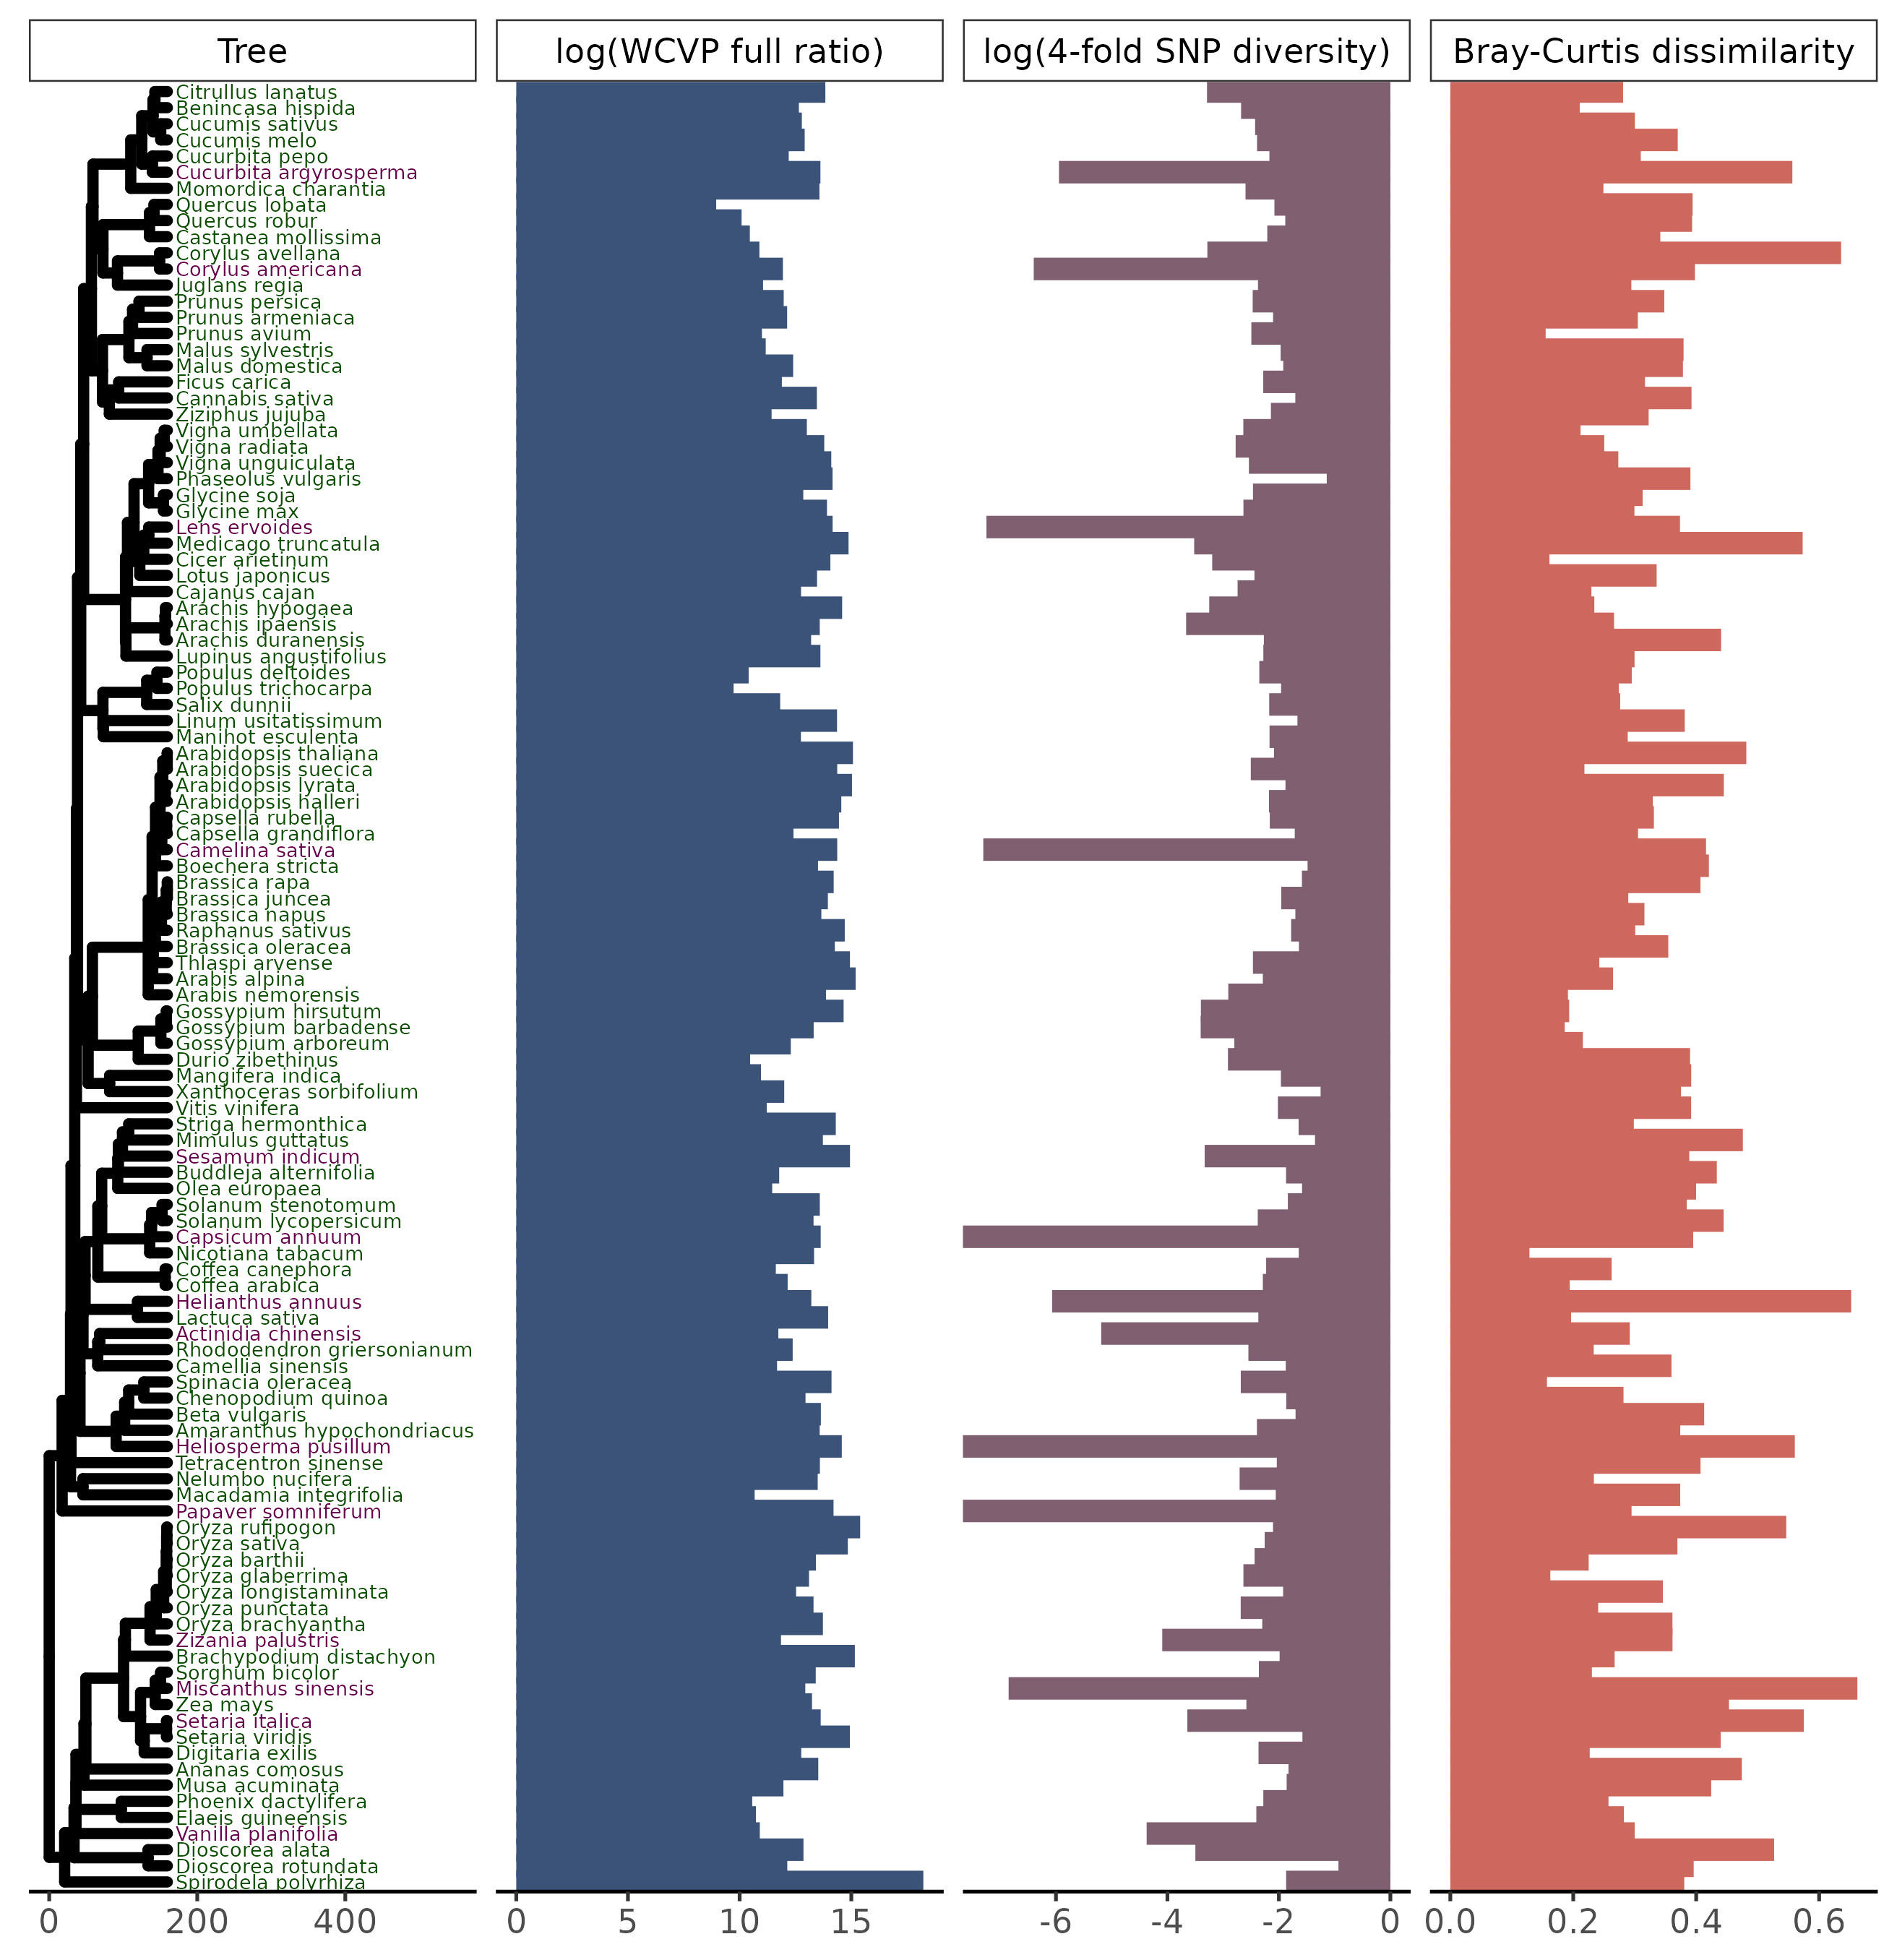
\includegraphics[width=0.98\textwidth]{figures/chapter_2/tree_with_primary_variables_2024-12-12.jpg}
    \caption{\textbf{Our study includes 112 plant species across a wide range of population sizes and diversity levels.} Species labeled in purple were considered outliers and omitted from downstream analyses (see Figure \ref{fig:pivskmer}), but species labeled in green were retained. The phylogenetic tree is scaled in millions of years. The WCVP full ratio is a unitless population size proxy equal to the ratio of range area, estimated using WCVP range maps, to squared plant height and is log-transformed (base 10, see Equation \ref{eq:proxy}). Nucleotide diversity is genome-wide average diversity at four-fold degenerate sites, log-transformed (base 10, see Equation \ref{eq:pi}). \textit{Capsicum annuum}, \textit{Heliosperma pusillum}, and \textit{Papaver somniferum} had nucleotide diversity values of zero and so have bars at the plotting limit (log(0) = $-\infty$). Bray-Curtis dissimilarity is average pairwise Bray-Curtis dissimilarity across all pairs of individuals in a species' sample (see Equation \ref{eq:braycurtis}).}
    \label{fig:phylo}
\end{figure}

Before testing our central hypothesis, we investigated whether technical sequencing variables could explain any of the diversity values observed in our dataset. Mean coverage correlated with both nucleotide diversity ($\rho$ = 0.33, p = 0.00033, Figure C3A) and $k$-mer diversity (Jaccard: $\rho$= -0.53, p = 2.6$\times10^{-9}$, Figure C3D; Bray-Curtis: $\rho$ = -0.34, p = 0.00021, Figure C3G). Coefficient of variation in bp sequenced correlated strongly with $k$-mer diversity (Jaccard: $\rho$ = 0.36, p = 0.00013, Figure C3E; Bray-Curtis: $\rho$ = 0.42, p = $4.7\times10^{-6}$, Figure C3H) but not nucleotide diversity ($\rho$ = -0.088, p = 0.36, Figure C3B). The number of individuals sequenced did not correlate with either nucleotide diversity or $k$-mer diversity (Figure C3C, C3F, C3I).

Given that mean coverage strongly correlated with both $k$-mer dissimilarity and nucleotide diversity, we decided to investigate this relationship further. We would expect that low coverage sequencing would produce artificially low nucleotide diversity and artificially high $k$-mer diversity. This is because our SNP-calling pipeline is generally tuned for high-coverage datasets (see \textbf{SNP calling pipelne}), so low coverage datasets produce few confident SNP calls. Conversely, low coverage sequencing only samples a small proportion of the total $k$-mer space in a set of reads. Thus, two independent low coverage samples are unlikely to share many $k$-mers in common and will have inflated $k$-mer diversity. Overall, we observed that species with very low mean coverage had both low nucleotide and high $k$-mer diversity (Figure \ref{fig:pivskmer}A, Figure C4A). In contrast, there was no clear mapping of these abnormal diversity values with coefficient of variation in base pairs sequenced (Figure C5) or the number of individuals sequenced (Figure C6). Based on these results, we removed 10 species from our dataset with mean coverage per individual $\leq$ 0.5x. This included three species (\textit{Capsicum annuum}, \textit{Heliosperma pusillum}, and \textit{Papaver somniferum}) with zero variant sites called because they had very low coverage (0.035x, 0.169x, 0.043x, respectively, Table S1). We also dropped 4 additional species with fewer than 1000 variant sites called: \textit{Camelina sativa
}, \textit{Sesamum indicum}, \textit{Setaria italica}, \textit{Actinidia chinensis}, the first of which were just slightly above our coverage cutoff (0.63x, 0.92x, 0.63x, respecitively, Table S1). These filtering steps removed many of the species with abnormally low diversity and high dissimilarity values excluding (Figure \ref{fig:pivskmer}B). In total, we kept data for 98 species for downstream hypothesis testing.

\end{double}

\begin{figure}
    \centering
    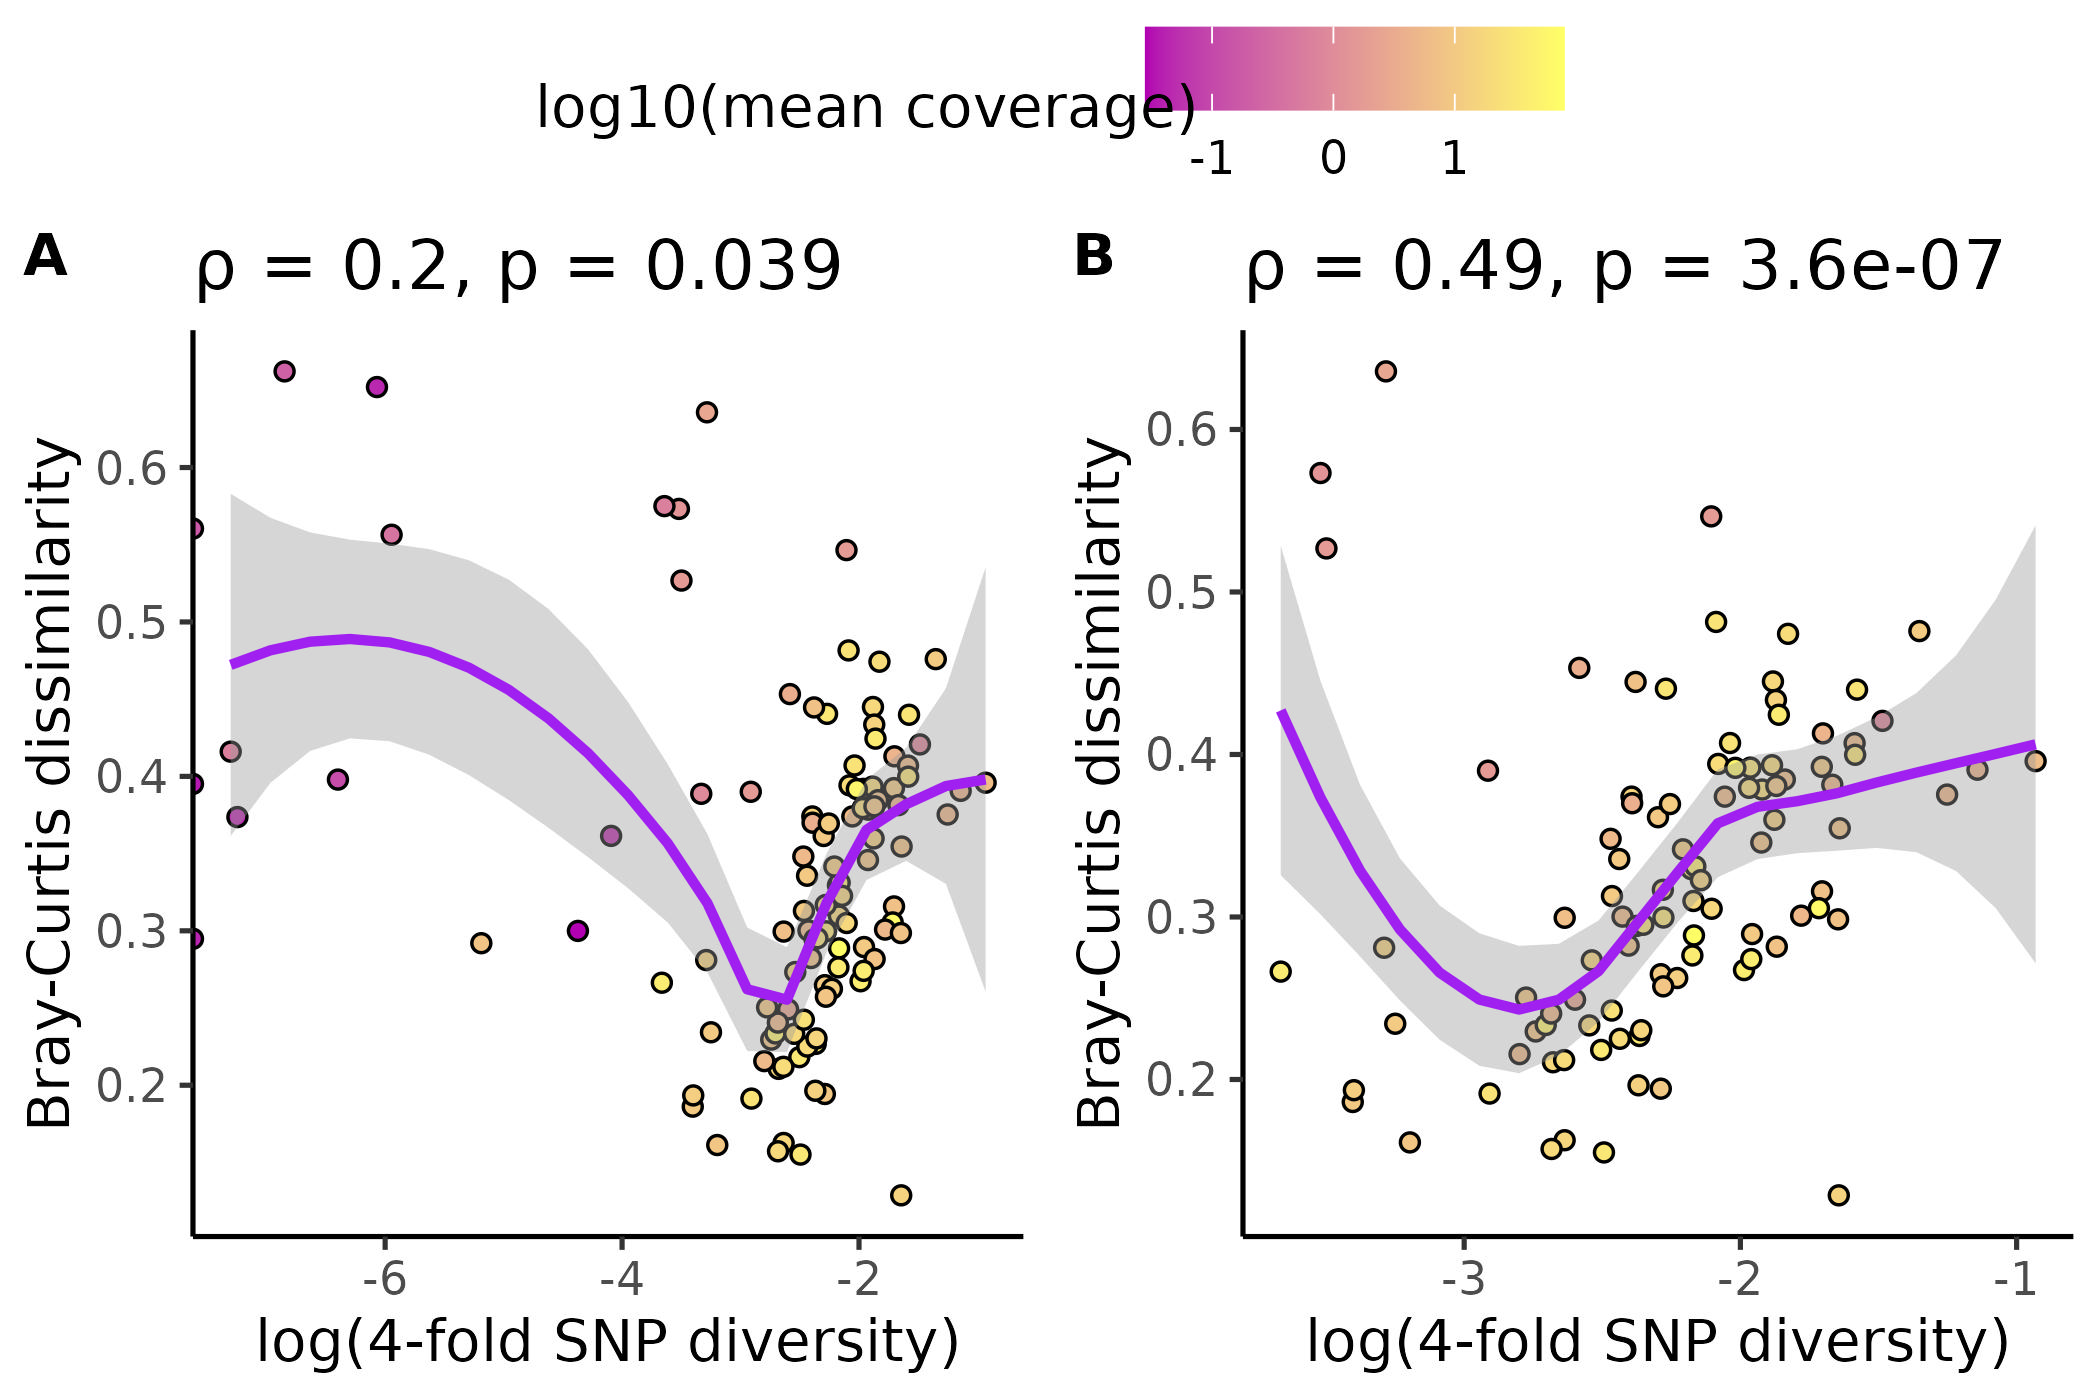
\includegraphics[width=\textwidth]{figures/chapter_2/pi_vs_bcd_high_vs_low_cov_2025-01-08.jpg}
    \caption{\textbf{Low coverage and low numbers of variant calls explains species with abnormally low diversity.} (A) shows the relationship between $k$-mer diversity and nucleotide diversity without omitting species with $\leq$ 0.5x coverage or $\leq$ 1000 SNP calls. (B) shows the same relationship, except species with $\leq$ 0.5x coverage or $\leq$ 1000 SNP calls are omitted. Each data point is a species. All species' points are colored by the log (base 10) of average genome-wide coverage per individual for that species. Purple lines are loess smoothing lines with 95\% confidence intervals shaded in gray. Values across the top of each plot are Spearman correlation coefficients ($\rho$) and p-values that test whether each correlation coefficient differs from zero.}
    \label{fig:pivskmer}
\end{figure}

\vspace{12pt}

\subsubsection*{Range size-squared height ratio varies over more orders of magnitude than nucleotide diversity}

\begin{double}

We next investigated whether Lewontin's paradox applied to our dataset by comparing diversity estimates against population size proxies. For each species, we estimated range size using either GBIF occurrence data or WCVP range maps. Estimates from these two methods were significantly correlated no matter whether invaded ranges (as defined in the WCVP range maps) were included ($\rho$ = 0.31, p = 0.00096, Figure C7A) or excluded ($\rho$ = 0.48, p = 7.3$\times10^{-8}$, Figure C7B). The omission of invaded ranges lowered the range size of several plant species based on WCVP range maps (Figure C7C) but had less effect on ranges estimated from GBIF occurrence data (Figure C7D). 

We then calculated the ratio of range size to squared plant height (Equation \ref{eq:proxy}) using height values from the EOL. We used this ratio as our primary population size proxy in downstream analyses. After excluding species with $< 0.5$x coverage and $< 1000$ variant sites called (Figure \ref{fig:pivskmer}), nucleotide diversity varied over about 4 orders of magnitude for the species in our dataset (from 0.00021 to 0.117, Table S2), while the ratio of range size to squared plant height based on WCVP and GBIF range estimation methods (including both native and invaded ranges) varied over 10 (from $8.9\times10^8$ to $1.7\times10^{18}$) and 13 (from $8.6\times10^5$ to $1.5\times10^{18}$) orders of magnitude, respectively (Table S2). Mean pairwise Bray-Curtis dissimilarity values varied about 4.9-fold across species, from 0.13 to 0.64, while mean pairwise Jaccard dissimilarity varied about 22-fold, from 0.040 to 0.87 (Table S2). Bray-Curtis dissimilarity values correlated with Jaccard dissimilarity values across species ($\rho = 0.76$, p $< 2.2\times10^{-16}$, Figure C8). 

\end{double}

\vspace{12pt}

\subsubsection*{$k$-mer diversity scales with population size proxies more than nucleotide diversity}

\begin{double}
    
The core of Lewontin's paradox is that a population's diversity does not scale much with population size. If $k$-mers capture a wider range of genetic variation compared to SNPs, population size will scale more with $k$-mer diversity than nucleotide diversity. If we did not control for shared evolutionary history or any confounding variables (mating system, life cycle habit, cultivation status, or genome size), then none of our diversity measures significantly correlated with the range size-squared height ratio (Figure C9). After controlling for confounding variables, nucleotide diversity marginally scaled with the range size-squared height ratio ($\beta =  0.14$, SE = 0.056, p = 0.017, Figure C10A). However, the relationship between $k$-mer diversity and the range size-squared height ratio was highly significant, with generally a greater slope (Jaccard: $\beta = $ 0.64, SE = 0.096 p = $2.2\times10^{-9}$, Figure C10B; Bray-Curtis dissimilarity: $\beta = $0.79, SE = 0.11, p = $7.3\times10^{-11}$, Figure C10C). We observed the same qualitative trend when we included both native and invaded ranges in the range size-squared height ratio (Figure C10D-F), or used the GBIF-based range estimates instead of WCVP-based estimates (Figure C11). Interestingly, we often observed Bray-Curtis dissimilarity having a larger slope with the range size-squared height ratio compared to Jaccard dissimilarity ($\beta = 0.64$ vs 0.79 Figure C10B-C), but models where Bray-Curtis dissimilarity was the response variable generally had lower adjusted $R^2$ (e.g. $R^2$ = 0.51 vs 0.41, models 2 and 3 in Table S4).

We also analyzed range size and plant height separately as population size proxies (Figure C12-C14). Overall, WCVP-estimated range size significantly affected nucleotide diversity ($\beta = 0.29$, SE = 0.072, p = 0.00011, Figure C12A) and $k$-mer diversity (Jaccard: $\beta = 0.92$, SE = 0.13, p = 9.9$\times10^{-11}$, Figure C12B; Bray-Curtis: $\beta = 1.2$, SE = 0.13,p = 3.2$\times10^{-14}$, Figure C12C), and this trend held when we estimated range size from GBIF occurrences (Figure C13A-C) or included invaded range area (Figure C12D-F and Figure C13D-F). On the other hand, nucleotide diversity did not scale with plant height ($\beta$ = 0.13, SE = 0.19, p = 0.5, Figure C14A), but $k$-mer diversity marginally scaled downward with plant height  (Jaccard: $\beta = -0.78$, SE =0.38, p = 0.046, Figure 14B; Bray-Curtis: $\beta = -0.77$, SE = 0.44, p = 0.088, Figure C14C).

Finally, we repeated our partial phylogenetic regressions controlling for genome size as an additional covariate. In this case, nucleotide diversity did not scale with the range size-squared height ratio ($\beta$ = 0.035, SE = 0.063, p = 0.58, Figure \ref{fig:popvdivgenome}A), but $k$-mer diversity did (Jaccard: $\beta = 0.54$, SE = 0.093,
p = $8.8\times10^{-8}$, Figure C15; Bray-Curtis: $\beta$ = 0.7, SE = 0.098, p = 2.2$\times10^{-10}$, Figure \ref{fig:popvdivgenome}B). Again, we got qualitatively similar results when we excluded invaded ranges in our range size estimates (Figure C16), used GBIF occurrences to estimate range size-squared height ratio (Figure C17) or used WCVP range size as the population size proxy (Figure C18). However, GBIF range size by itself did not scale with Jaccard dissimilarity (Figure C19B, C19E). Increased plant height associated with decreased $k$-mer diversity, but had no significant relationship with nucleotide diversity (Figure C20).

\begin{figure}
    \centering
    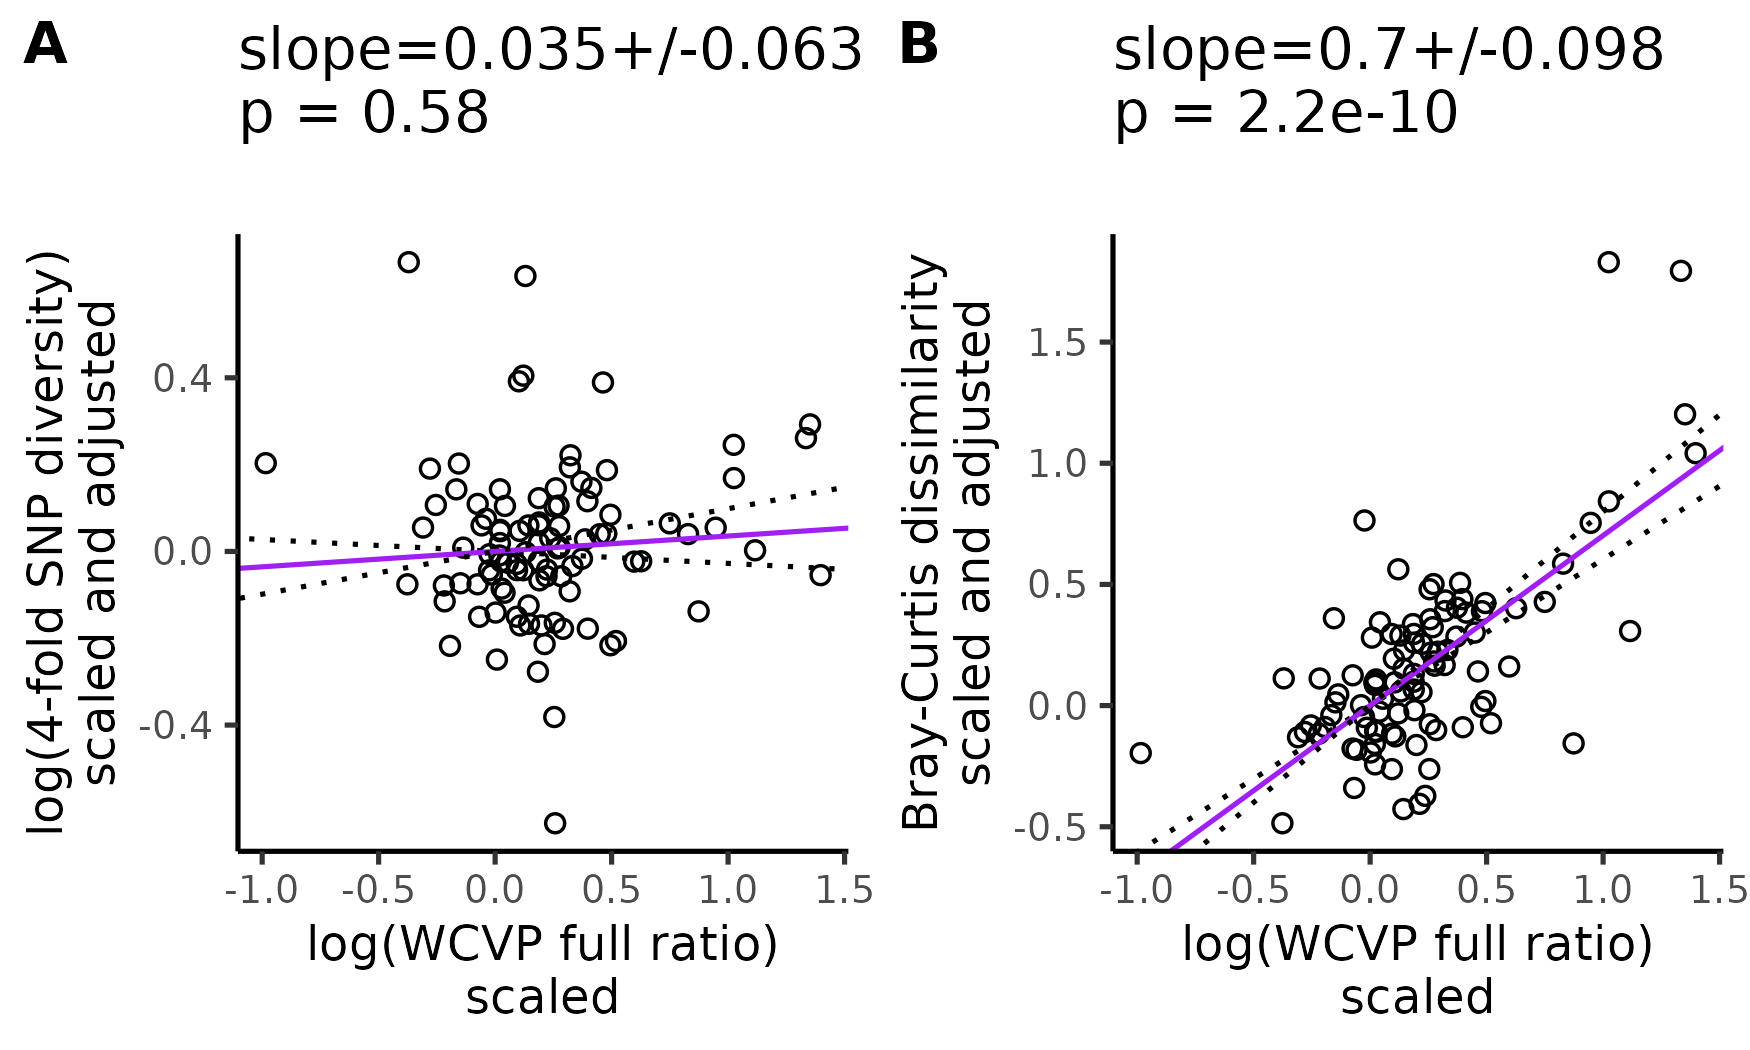
\includegraphics[width=\textwidth]{figures/chapter_2/wcvp_all_popsize_vs_pi_and_bcd_genome-size-corrected_2024-12-12.jpg}
    \caption{\textbf{$k$-mer diversity scales with population size proxies after controlling for genome size, life cycle habit, mating system, and cultivation status.} Purple lines are partial phylogenetic regression lines between diversity levels and the population size proxy. The y-axis (diversity) is scaled and adjusted according to Equation \ref{eq:partial}:  scaling diversity levels to a standard normal distribution, followed by correcting for phylogenetic relatedness and adjusting for the confounding variables (genome size, life cycle habit, mating system, and cultivation status). The values at the top of each plot give the slope of the partial regression $\pm$ one standard error and p-values testing whether the slopes differ from zero. Dotted lines show the partial regression slope $\pm$ one standard error. WCVP full ratio is a population size proxy estimated as the ratio of range size recorded in WCVP range maps (including invaded ranges) to squared plant height.}
    \label{fig:popvdivgenome}
\end{figure}

\end{double}

\begin{double}

\subsubsection*{$k$-mer diversity scales with genome size more than nucleotide diversity}
    
We also investigated the relationship between diversity and genome size because we expected genome size to potentially play a role in the mechanism underlying the greater scaling of $k$-mer diversity with population size. Genome size is often a strong predictor of diversity \citep{lynch_origins_2003}. Among eukaryotes, variation in genome size is largely explained by variation in transposable element abundance \citep{flavell_genome_1974, kidwell_transposable_2002, lynch_origins_2003, munoz-diez_using_2012, tenaillon_genome_2011, nystedt_norway_2013, ibarra-laclette_architecture_2013}, which contribute substantially to the repetitive sequence content of genomes and increase the difficulty of aligning short reads to a reference genome (reviewed in \citet{goerner-potvin_computational_2018}). Thus, our expectation was that $k$-mer-based diversity measures are more sensitive to genome size variation compared to nucleotide diversity. 

Increasing genome size was associated with decreasing $k$-mer diversity (Jaccard: $\beta = -3.7$, SE = 0.42, p = 8.4$\times10^{-14}$, Figure C21; Bray-Curtis: $\beta = -4.2$, SE = 0.45, p = 4.5$\times10^{-15}$, Figure \ref{fig:popvgenome}B) and nucleotide diversity ($\beta -1.8$, SE = 0.29, p = $1.4\times10^{-8}$, Figure \ref{fig:popvgenome}A), after controlling for variation in the range size-squared height ratio, mating system, life cycle habit, cultivation status, and evolutionary history. We got qualitatively similar results when the population size proxy we corrected for excluded invaded ranges (Figure C22), or if our population size proxy was based on GBIF occurrences (Figure C23), or we used range size or plant height individually to control for population size variation (Figure C24-C26). Across all of these analyses, the partial regression relationship between genome size and diversity was always significantly negative.

\begin{figure}
    \centering
    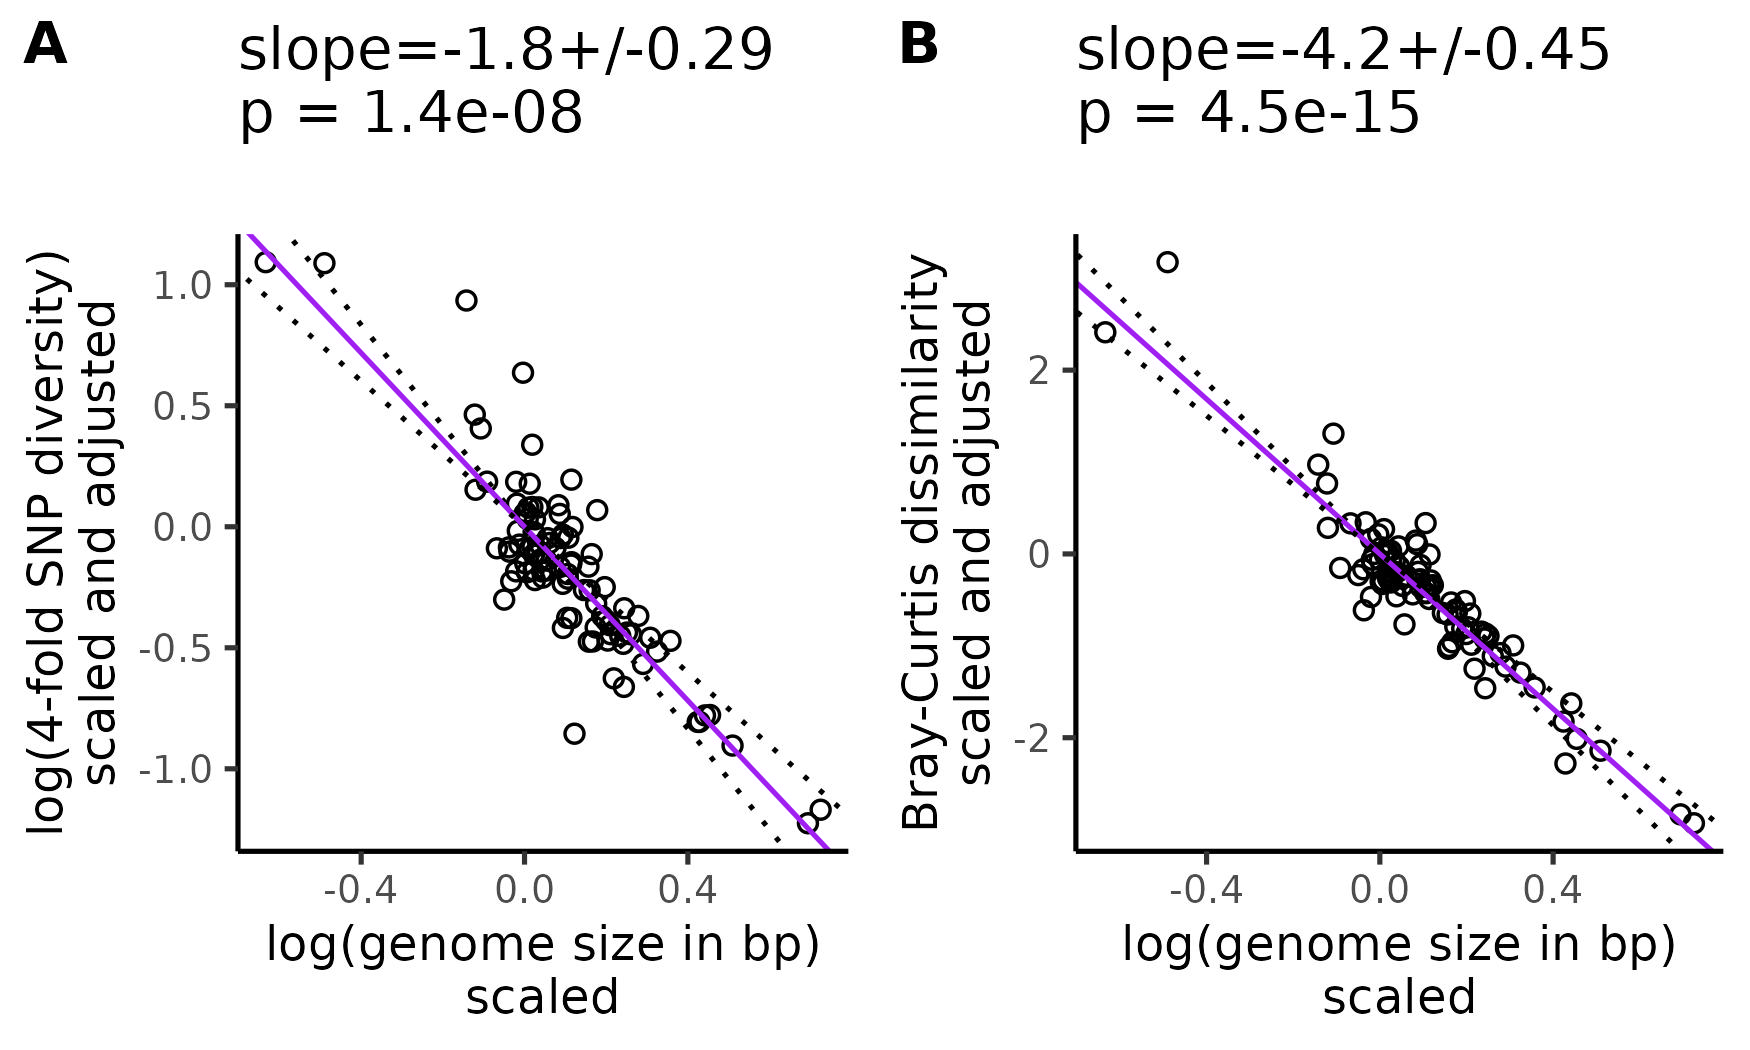
\includegraphics[width=\textwidth]{figures/chapter_2/pi_bcd_vs_genome_size_wcvp-all-corrected_2024-12-12.jpg}
    \caption{\textbf{$k$-mer diversity is more sensitive to genome size variation than nucleotide diversity.} Purple lines are partial phylogenetic regression lines between diversity levels and genome size (see Equation \ref{eq:partial}) after scaling diversity levels to a standard normal distribution (mean = 0, variance = 1), followed by scaling diversity levels and population sizes according to their phylogenetic relatedness, and finally adjusting for the confounding effects of mating system, cultivation status, life cycle habit, and population size. Here we used the ratio of range size to squared plant height, where range size was estimated from ranges in WCVP range maps (including invaded ranges). The values at the top of each plot give the slope of the partial regression $\pm$ one standard error and p-values testing whether the slopes differ from zero. Dotted lines show the partial regression slope $\pm$ one standard error.}
\label{fig:popvgenome}
\end{figure}

\end{double}

\begin{double}

\vspace{4pt}

\subsection*{Discussion}
%\addcontentsline{toc}{subsubsection}{2.4: Discussion}

Our goal was to investigate whether genomic approaches that can capture more genetic variation than reference-based methods can improve the scaling between population size proxies and diversity. This was motivated by literature suggesting suggesting SNPs called against a single reference provide an incomplete picture of genome-wide polymorphism \citep{schmidt_unbiased_2021, vanwallendael_alignment-free_2022, jaegle_extensive_2023, sopniewski_estimates_2024}. In total, we processed $>$205 terabases of publicly available sequencing data from the SRA over approximately 12 months of wall time, split between a maximum of 512 cores and 50 TB of disk space. After careful accounting for potential technical and phylogenetic confounding, the standardized slope between $k$-mer-based diversity and the range size-squared height ratio was up to 20 times larger than the same standardized slope for nucleotide diversity ($\beta =$ 0.035 vs 0.7, Figure \ref{fig:popvdivgenome}). We observed similar results across the two different measures of range size (Figure C17) and $k$-mer diversity (Figure C15). We also observed that $k$-mer-based diversity is more sensitive to variation in genome size compared to nucleotide diversity (Figure \ref{fig:popvgenome}). Overall, these results are consistent with the possibility that  diversity missed by reference-based analyses or changes in the diversity calculation itself can partly explain the weak scaling between population size and diversity. However, a larger pangenome scale analysis will be required to fully understand the genetic variants underlying this result.

Extending our findings to Lewontin's paradox directly is complicated by a few factors. First, it would be ideal to compare our diversity estimates to neutral expectations of diversity vs population size. For SNPs, the expected diversity under neutrality would be $4N_e\mu$ or a similar formula. For $k$-mers the exact value of $\mu$ is not clear, as $k$-mers also reflect non-SNP variation. Several $k$-mer-based measures of diversity are nearly perfectly correlated with $\pi$ in neutral models where only SNPs are considered \citep{roberts_k-mer-based_2024}, but the inclusion of non-SNP variation would probably change this relationship. Identifying the concrete variants underlying $k$-mers would help us better understand $\mu$ for $k$-mer, but this is currently not possible for mutations other than SNPs and small indels without pangenomic references \citep{uricaru_reference-free_2015, gauthier_discosnp-rad_2020}. The eventual release of pangenomic references across many species will provide better context for increased scaling of $k$-mer diversity with population size. Similar to previous Lewontin's paradox studies, we also use both non-coding sequences (for k-mers) and 4-fold degenerate sites (for SNPs) as standards for estimating neutral diversity \citep{leffler_revisiting_2012, buffalo_quantifying_2021}, but there could be differences between coding and non-coding values of $\mu$ that contribute to results observed in our work and previous work. More estimates of $\mu$ are needed for non-SNP mutations \citep{quiroz_causes_2023}, but we further caution that many estimates of $\mu$ will be limited in that they usually reflect contemporary populations. Variation in $\mu$ over time, such as through TE bursts \citep{belyayev_bursts_2014}, could play an important role in diversity vs population size scaling and warrant further research. 

In addition to limitations estimating $\mu$ and $\pi$, estimates of $N_e$ also tend to be limited in investigations of Lewontin's paradox. Like previous analyses, our analysis assumes that contemporary population size estimates are good proxies for historic population sizes \citep{corbett-detig_natural_2015, buffalo_estimating_2020}. Common population size proxies such as range size and plant height only reflect the current census population size of a species. However, it is  the long-term harmonic mean of the effective population size, not just the current size, that determines diversity levels within a population \citep{wright_breeding_1940}. There is some literature correlating aspects of species history with contemporary diversity levels \citep{lopezdelgado_history_2022} and incorporating these metrics into Lewontin's paradox is an exciting avenue for future research. As a first step in this direction, we used plant range maps into native and invaded ranges to test the robustness of our results to invasion-related range size changes \citep{brown_rwcvp_2023}. Overall, our observations were remarkably similar no matter whether we included or excluded invaded ranges in our population size proxies (Figure C17A-C vs Figure C17D-F). Part of this apparent robustness was due to the insensitivity of our GBIF-based range size estimates to the inclusion of invaded ranges (Figure C7D). However, our WCVP-based range size estimates were drastically altered by the inclusion of invaded ranges (Figure C7C) and still yielded similar results (Figure \ref{fig:popvdivgenome}, C15, C16). Although we cannot rule out the possibility that older historical events have affected contemporary diversity levels, our results appear to be robust to recent biological invasions.

As with all regression-based analyses, our results are also ultimately sensitive to error in the measurement of both covariates (population size proxies, genome size, mating system, life cycle habit, or cultivation status) and outcome variables (nucleotide or $k$-mer diversity). For example, we did not filter out potentially contaminating sequences from our $k$-mer analysis, which could add noise to our $k$-mer dissimilarity values. However, this could only explain the increased scaling between $k$-mer diversity and population size if plants with larger population size proxies had a higher diversity of contaminants, which seems unlikely given that many of the sequencing datasets in our study are from laboratory cultivated plants (see Table S1) and that we excluded low-frequency $k$-mers from our analyses. Our study is also unique in the multiple steps we took to limit the influence of systematic measurement errors on our coefficients, including reanalyzing all population-level sequencing data with one pipeline to limit the impact of bioinformatic parameter choices on our analysis \citep{mirchandani_fast_2024}, filtering out low coverage datasets\citep{sandell_genomic_2022}, accounting for missing data in calculations of nucleotide diversity \citep{schmidt_unbiased_2021, korunes_pixy_2021}and estimating range size with two different methods (WCVP range maps and GBIF occurrence records, Figure C6). Although we could not control for some covariates \citep{willis_age_1922, romiguier_comparative_2014, guo_relationships_2024} due to a dearth of data, our study is still the largest reanalysis of population-level sequencing data in plants that we know of to date. The availability of our workflow also makes it easy for our study to be extended as more population-level sequencing data is released. 

Interestingly, the estimated effect of our population size proxies on diversity was often slightly larger for Bray-Curtis dissimilarity than Jaccard dissimilarity (for example, $\beta = 0.7$ vs 0.54 from Figure \ref{fig:popvdivgenome}B vs Figure C15, Table S4). In contrast, the range size-squared height ratio was often slightly more predictive of Jaccard dissimilarity than Bray-Curtis dissimilarity (Table S4). We could not test whether these trends were statistically significant, but the benefits of different $k$-mer metrics in predicting measures of population size warrant further study. Our expectation is that $k$-mer diversity measures based on frequency, such as Bray-Curtis dissimilarity, better capture diversity compared to measures based on purely $k$-mer presence/absence, such as Jaccard dissimilarity, because they explicitly measure copy number variation. However, accurately measuring $k$-mer frequencies likely requires higher sequencing coverage than calling presence/absence, which could explain why Bray-Curtis dissimilarity generally scaled more with population size but had a lower $R^2$ compared to Jaccard dissimilarity (Table S4). Future studies using higher coverage population level sequencing data could help test this hypothesis.  

$k$-mer frequencies are known to be highly informative of genomic structure, with one common application of $k$-mers being the estimation of genome size \citep{vurture_genomescope_2017, pflug_measuring_2020}. Similar to previous studies, we observed that nucleotide diversity was negatively correlated with genome size \citep{lynch_origins_2003, chen_genetic_2017}, but we observed an even stronger negative correlation for $k$-mer diversity ($\beta = -1.8$, SE = 0.29 vs $\beta = $ -3.7, SE = 0.42 in Figure \ref{fig:popvgenome}). $k$-mers also appeared to explain diversity patterns that scaled with population size beyond those explained by genome size, while nucleotide diversity did not. After controlling for genome size, the relationship between our population size proxies and nucleotide diversity was not significant (Figure \ref{fig:popvdivgenome}A, C17-C19 panels A and D), but the relationship between $k$-mer diversity and population size proxies was often still highly significant (Figure \ref{fig:popvdivgenome}B, C17-C19 panels B; C; E; F). The only exception was that Jaccard dissimilarity did not significantly scale with GBIF-based estimates of range size (Figure C19B, C19E). This additional scaling of $k$-mer diversity with population size beyond just the effects of genome size and confounding variables suggests that $k$-mers capture some element of the population size-diversity relationship that is absent from nucleotide diversity.

Our results do not negate the fact that other important factors also underlie Lewontin's paradox, such as past demographic fluctuations and linked selection. However, our results do suggest that future studies of Lewontin's paradox may want to consider diversity outside one reference genome. The increasing availability of pangenomes across species \citep{goktay_new_2021, zhou_graph_2022, rice_pangenome_2023, wang_pangenome_2023} offers many opportunities to revisit this classic population genetics question. Ideal future studies would use pangenomic genotyping methods across a wide range of species with a standardized pipeline, combined with multiple proxies of population size, and understandings of each species' demographic history. Altogether, these methodological developments will hopefully reveal a more wholistic picture of variation across the tree of life.  

\vspace{4pt}

\subsection*{Data availability}
    
Supplemental figures are in appendix C. Our entire analysis is packaged as a snakemake workflow stored here: \href{https://github.com/milesroberts-123/tajimasDacrossSpecies}{https://github.com/milesroberts-123/tajimasDacrossSpecies}. All supplementary tables will be made available online at \textit{Evolution Letters}. Table S1 contains the metadata for all of the datasets used in this study, including sources for genome assemblies, genome annotations, population-level sequencing datasets, and GBIF observations. Table S2 contains all of the covariate and response variable values used for fitting our phylogenetic least squares models. Table S3 contains the estimated coefficients of all of our phylogenetic least squares models and their related statistics, including p-values and standard errors. Table S4 contains the model-level statistics for each phylogenetic least squares model, including $R^2$ values and F-test results. 

\end{double}

\newpage

\section*{CHAPTER 3: $k$-MER-BASED APPROACHES TO BRIDGING PANGENOMICS AND POPULATION GENETICS\footnote{This chaper is published at the following DOI under a Creative Commons CC BY License: \url{https://doi.org/10.1093/molbev/msaf047}. This license permits unrestricted use, distribution, and reproduction in any medium, provided the original work is properly cited. Permission to reuse this article is not required.}}
\addcontentsline{toc}{subsection}{CHAPTER 3: \textit{k}-MER-BASED APPROACHES TO BRIDGING PANGENOMICS AND POPULATION GENETICS}

\setcounter{figure}{0}
\renewcommand{\figurename}{Figure}
\renewcommand{\thefigure}{3.\arabic{figure}}

\setcounter{equation}{0}
\renewcommand{\theequation}{3.\arabic{equation}}

\begin{double}

\vspace{4pt}

\subsection*{Abstract}

Many commonly studied species now have more than one chromosome-scale genome assembly, revealing a large amount of genetic diversity previously missed by approaches that map short reads to a single reference. However, many species still lack multiple reference genomes and correctly aligning references to build pangenomes can be challenging for many species, limiting our ability to study this missing genomic variation in population genetics. Here, we argue that $k$-mers are a very useful but underutilized tool for bridging the reference-focused paradigms of population genetics with the reference-free paradigms of pangenomics. We review current literature on the uses of $k$-mers for performing three core components of most population genetics analyses: identifying, measuring, and explaining patterns of genetic variation. We also demonstrate how different $k$-mer-based measures of genetic variation behave in population genetic simulations according to the choice of $k$, depth of sequencing coverage, and degree of data compression. Overall, we find that $k$-mer-based measures of genetic diversity scale consistently with pairwise nucleotide diversity ($\pi$) up to values of about $\pi = 0.025$ ($R^2 = 0.97$) for neutrally evolving populations. For populations with even more variation, using shorter $k$-mers will maintain the scalability up to at least $\pi = 0.1$. Furthermore, in our simulated populations, $k$-mer dissimilarity values can be reliably approximated from counting bloom filters, highlighting a potential avenue to decreasing the memory burden of $k$-mer based genomic dissimilarity analyses. For future studies, there is a great opportunity to further develop methods to identifying selected loci using $k$-mers.

\vspace{4pt}

\subsection*{Introduction}
%\addcontentsline{toc}{subsubsection}{3.1: Introduction}

Two decades ago, assembling one reference genome for one eukaryotic species was an international, herculean effort \citep{venter_sequence_2001}. Now, individual laboratories can readily assemble and align multiple reference-quality genomes from the same species into pangenomes \citep{golicz_pangenomics_2020}. This shift toward pangenomes as the basis for genetic studies is already transforming our understanding of genetic variation in populations. Analysis of pangenomes has uncovered vast quantities of genetic variation previously missed by the ubiquitous practice of aligning short reads to a single reference genome \citep{wong_towards_2020, siren_pangenomics_2021, ebler_pangenome-based_2022, zhou_graph_2022, rice_pangenome_2023, liao_draft_2023}, increased the power of trait mapping \citep{song_eight_2020, chin_multiscale_2023}, and resolved complex structural variations \citep{hickey_genotyping_2020, song_new_2024}. Pangenomes have even revised our understanding of previously cataloged variation, because single nucleotide polymorphisms (SNPs) once identified by mapping reads against a single reference can sometimes be resolved as alignment errors due to structural variation \citep{jaegle_extensive_2023}. Altogether, pangenomes provide a more accurate representation of genetic variation, reducing the commonly observed phenomenon where one's choice of reference genome shapes the ultimate conclusions of a study (i.e. reference bias, \citet{gage_multiple_2019, gunther_presence_2019, chen_reference_2021, ebler_pangenome-based_2022}). This better ability to capture and explain patterns of genetic variation, combined with recent developments in pangenome assembly algorithms  \citep{garrison_building_2024, hickey_genotyping_2020} and an explosion in pangenome sequencing for many non-model organisms \citep{lei_plant_2021}, means that pangenomes will likely be the standard for population genetics analysis in the near future.

However, pangenomes can be difficult to assemble and tune in some contexts \citep{hahn_molecular_2018, song_new_2024}. First, pangenomes by definition require more sequencing data to assemble compared to a single reference genome, which can make building pangenomes expensive for large genome species or study systems with fewer resources. Furthermore, whole genome alignment (WGA) is key for pangenome assembly but also difficult to tune, affecting pangenome analysis. Modern WGA algorithms are impressive and are being used to produce pangenomes for a wide range of species \citep{garrison_building_2024}; however, current WGA algorithms are mainly developed and tuned to align human and model species genomes, and so do not always generalize well to genomes that are large, highly repetitive, highly diverse, polyploid, or containing high levels of structural variation (reviewed in \citet{song_new_2024}). For example, corn (\textit{Zea mays}) has a famously repetitive and structurally variable genome and new WGA approaches needed to be developed just to properly align corn genomes \citep{song_anchorwave_2022}. There are also still many open questions on how to best represent complex, nested variations in such alignments and tune alignment parameters  \citep{song_new_2024}. A researcher's exact choice of alignment parameters and software can drastically affect the shape of a pangenome graph \citep{rice_pangenome_2023} and downstream genotype calls \citep{Orawe_low_2013, Li_toward_2014, bush_genomic_2020, Betschart_comparison_2022, sopniewski_estimates_2024}. Given the challenges of computing and tuning alignments, approaches that skip alignment altogether could valuably complement or help guide pangenome assembly. 

In this review we argue that the $k$-mers deserve more attention from population geneticists because they can complement the study of pangenomes. A $k$-mer is a sub-sequence of length $k$ within a larger sequence. For example, the sequence ``ATGCA'', contains the unique 2-mers AT, TG, GC, and CA. The main benefit of $k$-mers is that they can be analyzed without alignment. Instead, one simply counts all of the unique $k$-mers present in a sample of reads (where $k$-mers that are reverse complements of each other are typically considered identical and are counted together \citet{kokot_kmc_2017}), then uses the resulting count matrix for downstream analysis (see Figure \ref{fig:kvs}). Thus, $k$-mers derived from regions far diverged, absent, or otherwise unalignable in a given reference will not be automatically excluded from an analysis, allowing one to get a picture of pangenomic variation. 
$k$-mers have a long history of use in metagenomics \citep{mcclelland_selection_1985, rosen_metagenome_2008, dubinkina_assessment_2016}, phylogenetics \citep{kolekar_alignment-free_2012, Haubold_alignment-free_2014, zielezinski_alignment-free_2017, zielezinski_benchmarking_2019, bussi_large-scale_2021, beichman_evolution_2023, jenike_guide_2024}, computer science \citep{shannon_mathematical_1948}, and quantitative genetics \citep{voichek_identifying_2020, kim_dissecting_2020, Gupta_gwas_2021, Onetto_population_2022, lemane_kmdiff_2022}. However, while applications of $k$-mers receive much attention in other disciplines, population genetic investigations using $k$-mers remain limited. 

Our goal is to review $k$-mer-based approaches for identifying, measuring, and explaining patterns of genetic variation in populations. At the same time, we investigate the behavior of $k$-mer-based measures of variation to the choice of $k$, the depth of sequencing coverage, and the degree of data compression. We finally highlight some avenues to explore in $k$-mer-based (i.e. reference-free or alignment-free) population genetics. Overall, we advocate that $k$-mer-based approaches can be valuable complements to common reference-based population genetics methods.

\vspace{4pt}

\subsection*{Box 1: What is the ``best'' value for $k$?}
    
A common first question in $k$-mer based analyses is: What value(s) of $k$ should be analyzed?  The ``best'' $k$ for an analysis is ultimately determined by a trade-off between the length of $k$ and sequencing error: longer $k$-mers are more likely to represent unique genomic sequences, but are also more likely to contain a sequencing error \citep{rahman_association_2018}. In practice, many studies use a $k$ of around 20-40 bp \citep{ponsero_comparison_2023} because $k$-mers in this range can be reliably sequenced with short read data and often align uniquely to their source genome \citep{wu_effect_1991,becher_measuring_2022}. For example, $k = 32$ captures 85.7 \% of unique sequences in the human genome \citep{shajii_fast_2016}, while $k = 21$ distinguishes many eukaryote, bacteria, and archea species \citep{bussi_large-scale_2021}. However, there are many past studies that propose criteria for choosing specific values of $k$.

\vspace{4pt}

\subsection*{Choosing multiple values of $k$}

One ``brute force'' approach to test the sensitivity of results to $k$ is to simply repeat an analysis multiple times for different values of $k$. This approach is especially common among genome assembly algorithms \citep{chikhi_informed_2014, durai_informed_2016} but could be applied to almost any analysis in theory. The main drawback, however, is the high computational burden of performing the same analysis multiple times. It is also difficult to know without more information whether analyses performed for certain values of $k$ produce more accurate results than analyses for other values of $k$, motivating the need for $k$ selection criteria that can be either minimized or maximized.  

\vspace{4pt}

\subsection*{Choosing $k$ based on the number of unique non-erroneous $k$-mers}

Higher values of $k$ generally allow greater detection of unique sequences, but increase the probability of observing $k$-mers containing at least one sequencing error \citep{chikhi_informed_2014, rahman_association_2018}. Each sequencing error can result in up to $k$ erroneous $k$-mers, making it important to prevent errors from dominating one's analysis. Thus, choosing a $k$ that maximizes the number of unique non-erroneous $k$-mers in a dataset is generally considered optimal for tasks like genome assembly \citep{chikhi_informed_2014}. This approach generally involves measuring the $k$-mer frequency spectrum and then fitting a model to the distribution to estimate which parts of the spectrum come from erroneous $k$-mers \citep{chikhi_informed_2014}. Usually,  the low-frequency end of the spectrum is dominated by erroneous $k$-mers because sequencing errors are unlikely to generate the same erroneous $k$-mers many times and usually convert real $k$-mers into $k$-mers not found in the source genome \citep{kelley_quake_2010}. Although this criterion for choosing $k$ could be applied to population genetic datasets, it is not if clear the resulting optimal $k$ would vary significantly between genomes within the same species. Presumably, if genomes within the same species have considerable variation in repetitive content \citep{haberer_european_2020}, size \citep{schmuths_genome_2004}, or ploidy (reviewed in \citet{kolar_mixed-ploidy_2017}) then the optimal $k$ could vary. Determining the value of $k$ that maximizes the number of unique non-erroneous $k$-mers across all individuals in a population may be of interest for future population genetics studies.

\vspace{4pt}

\subsection*{Choosing $k$ based on the probability of chance $k$-mer matches between samples}

Another way to choose $k$ is to think about the probability that a $k$-mer from one genome is also found in a second genome by chance alone. For example, it would be unsurprising for almost any pair of reasonably long, naturally-occurring DNA sequences to share the $k$-mer ``AGC'' because this k-mer is very short and could occur many times in a random sequence. How large must $k$ be then before finding a $k$-mer in two different sequences is unlikely by chance alone? To discuss this question, we next present equations similar to ones in \citet{ondov_mash_2016}, except we generalize to account for variation in base composition between sequences being compared. 

Let's begin by imagining we have two genome sequences we wish to compare: $X_1$ and $X_2$. First, to generate $X_1$, we sample with replacement the letters A, T, G, and C a total of $L$ times with probabilities $p_{A1}$, $p_{T1}$, $p_{G1}$, and $p_{C1}$, respectively where $p_{A1} + p_{T1} + p_{G1} + p_{C1} = 1$. In other words, we sample our DNA from a multinomial distribution where we assume that each base is sampled independently of the preceding bases. This gives us one strand for $X_1$ and we can then generate the complementary strand by pairing A with T and G with C. We repeat this whole process once more to construct $X_2$ using probabilities $p_{A2}$, $p_{T2}$, $p_{G2}$, and $p_{C2}$, which may or may not match the probabilities for $X_1$, except we only sample $k$ bases. This gives us a $k$-mer, $K$, in the genome sequence of $X_2$. We now wish to find the probability that $K$ occurs in $X_1$, assuming that the sampling of bases for $K$ was independent of sampling bases for $X_1$.

If we imagine constructing $X_1$ and $K$ at the same time, then the probability of drawing the same letter for both sequences at a given position is: 

\begin{equation}
    \Sigma_F = p_{A1}p_{A2} + p_{T1}p_{T2} + p_{G1}p_{G2} + p_{C1}p_{C2}
\end{equation} 

However, we also want to consider sequences that are reverse complements as identical, so the probability of drawing a pair of bases that match as reverse complements is: 

\begin{equation}
    \Sigma_R = p_{A1}p_{T2} + p_{T1}p_{A2} + p_{G1}p_{C2} + p_{C1}p_{G2}
\end{equation} 

The probability of drawing $k$ pairs of bases in a row that are either identical or reverse complement matches is thus $\Sigma_F^k$ and $\Sigma_R^k$, respectively, assuming that each base is sampled independently of all others. The complementary probability of not getting $k$ matches in a row on the forward strand is $1 - \Sigma_F^k$ and, comparably, $1 - \Sigma_R^k$ for the reverse strand. Because $X_1$ contains $L$ bases, there are a total of $L - k + 1$ $k$-mers in $X_1$, so the probability of a $K$ not matching at any $k$-mers in $X_1$ is approximately $(1 - \Sigma_F^k)^{L - k + 1}$ and $(1 - \Sigma_R^k)^{L - k + 1}$. It should be noted that at this step we are assuming that the chance of $K$ mismatching at a given position in $X_1$ is independent of the chance that $K$ mismatches at other positions in $X_1$, which is not strictly true. For example, if $K$ is the sequence ``AAAAA" and we compare $K$ to a subsequence in $X_1$ that is ``AACAA" we would say that $K$ and this subsequence do not match. However, with this information we would also know with certainty that adjacent $k$-mers in $X_1$ will also not match $K$ because they will still contain a ``C". However, we will continue with assuming that the mismatch between $X_1$ and $K$ is independent at all positions because this makes our final equations more conservative (decreasing the $\Sigma_F^k$ term in Equation \ref{kfp_approx_f} will decrease the overall value of Equation \ref{kfp_approx_f}).

We can now say that the probability of finding the $k$-mer $K$ at least once by chance alone at any of the $L - k + 1$ positions in the sequence $X_1$ is:

\begin{equation} \label{kfp_complex_f}
    P(K \in X_{1F}) = 1 - \left(1 - \Sigma_F^k\right)^{(L - k + 1)}
\end{equation}

\begin{equation} \label{kfp_complex_r}
    P(K \in X_{1R}) = 1 - \left(1 - \Sigma_R^k\right)^{(L - k + 1)}
\end{equation}
Assuming $k << L$, Equations \ref{kfp_complex_f} and \ref{kfp_complex_r} approximate to:

\begin{equation} \label{kfp_approx_f}
    P(K \in X_{1F}) \approx 1 - \left(1 - \Sigma_F^k\right)^{L}
\end{equation}

\begin{equation} \label{kfp_approx_r}
    P(K \in X_{1R}) \approx 1 - \left(1 - \Sigma_R^k\right)^{L}
\end{equation}

We confirmed that equations \ref{kfp_approx_f} and \ref{kfp_approx_r} work as expected in simulations (Figure \ref{fig:equation-test}). Similar to \citet{fofanov_how_2004}, we can then solve these equations to give the minimum $k$-mer length required to achieve a desired probability of chance $k$-mer matching of $q = P(K \in X_{1F}) = P(K \in X_{1R})$:

\begin{equation} \label{eq:kfp_final_f}
    k_F = \left \lceil log_{\Sigma_F}\left(1 - (1 - q)^{1/L}\right) \right \rceil
\end{equation}

\begin{equation} \label{eq:kfp_final_r}
    k_R = \left \lceil log_{\Sigma_R}\left(1 - (1 - q)^{1/L}\right) \right \rceil
\end{equation}
and now given a choice of $q$ we are willing to tolerate, we can then use $\max(k_F, k_R)$ as a potential choice of $k$. 

Equations \ref{eq:kfp_final_f} and \ref{eq:kfp_final_r} demonstrates that $k = 19$ reduces the probability of two 3 Gb genomes of random sequence sharing the same $k$-mer by chance to just 1 \% \citep{ondov_mash_2016}  (assuming all bases are in equal proportion in both genomes, $p_{A1} = p_{T1} = p_{G1} = p_{C1} = p_{A2} = p_{T2} = p_{G2} = p_{C2} = 1/4$) while $k = 27$ gives $q = 1 \times 10^{-6}$ for a 10 Gb genome where both $X_1$ and $X_2$ have a GC conent of 42 \% ($p_{A1} = p_{T1} = p_{A2} = p_{T2} = 0.29$ and $p_{G2} = p_{C2} = p_{G2} = p_{C2} = 0.21$). Slightly longer $k$-mers are required when the proportion of each base is not 25 \% in both genomes because it is more likely then to have low-complexity strings of bases which make spurious matches more likely. For example, the required $k$-mer length increases to 34 bp if the GC content of both genomes is 21 \% ($p_{A1} = p_{T1} = p_{A2} = p_{T2} = 0.395$ and $p_{G1} = p_{C1} = p_{G2} = p_{C2} = 0.105$), given a 10 Gb genome and $q = 1 \times 10^{-6}$.

In summary, if $k$ is high enough, two genomes in a population are highly unlikely to share $k$-mers just through the accumulation of random sequences alone, suggesting that shared $k$-mers usually reflect shared ancestry. Developing additional $k$-mer selection criteria that explicitly model the influence of shared ancestry on the probability of $k$-mer sharing could improve approaches to choosing $k$.

\end{double}

\begin{figure}[H]
    \centering
    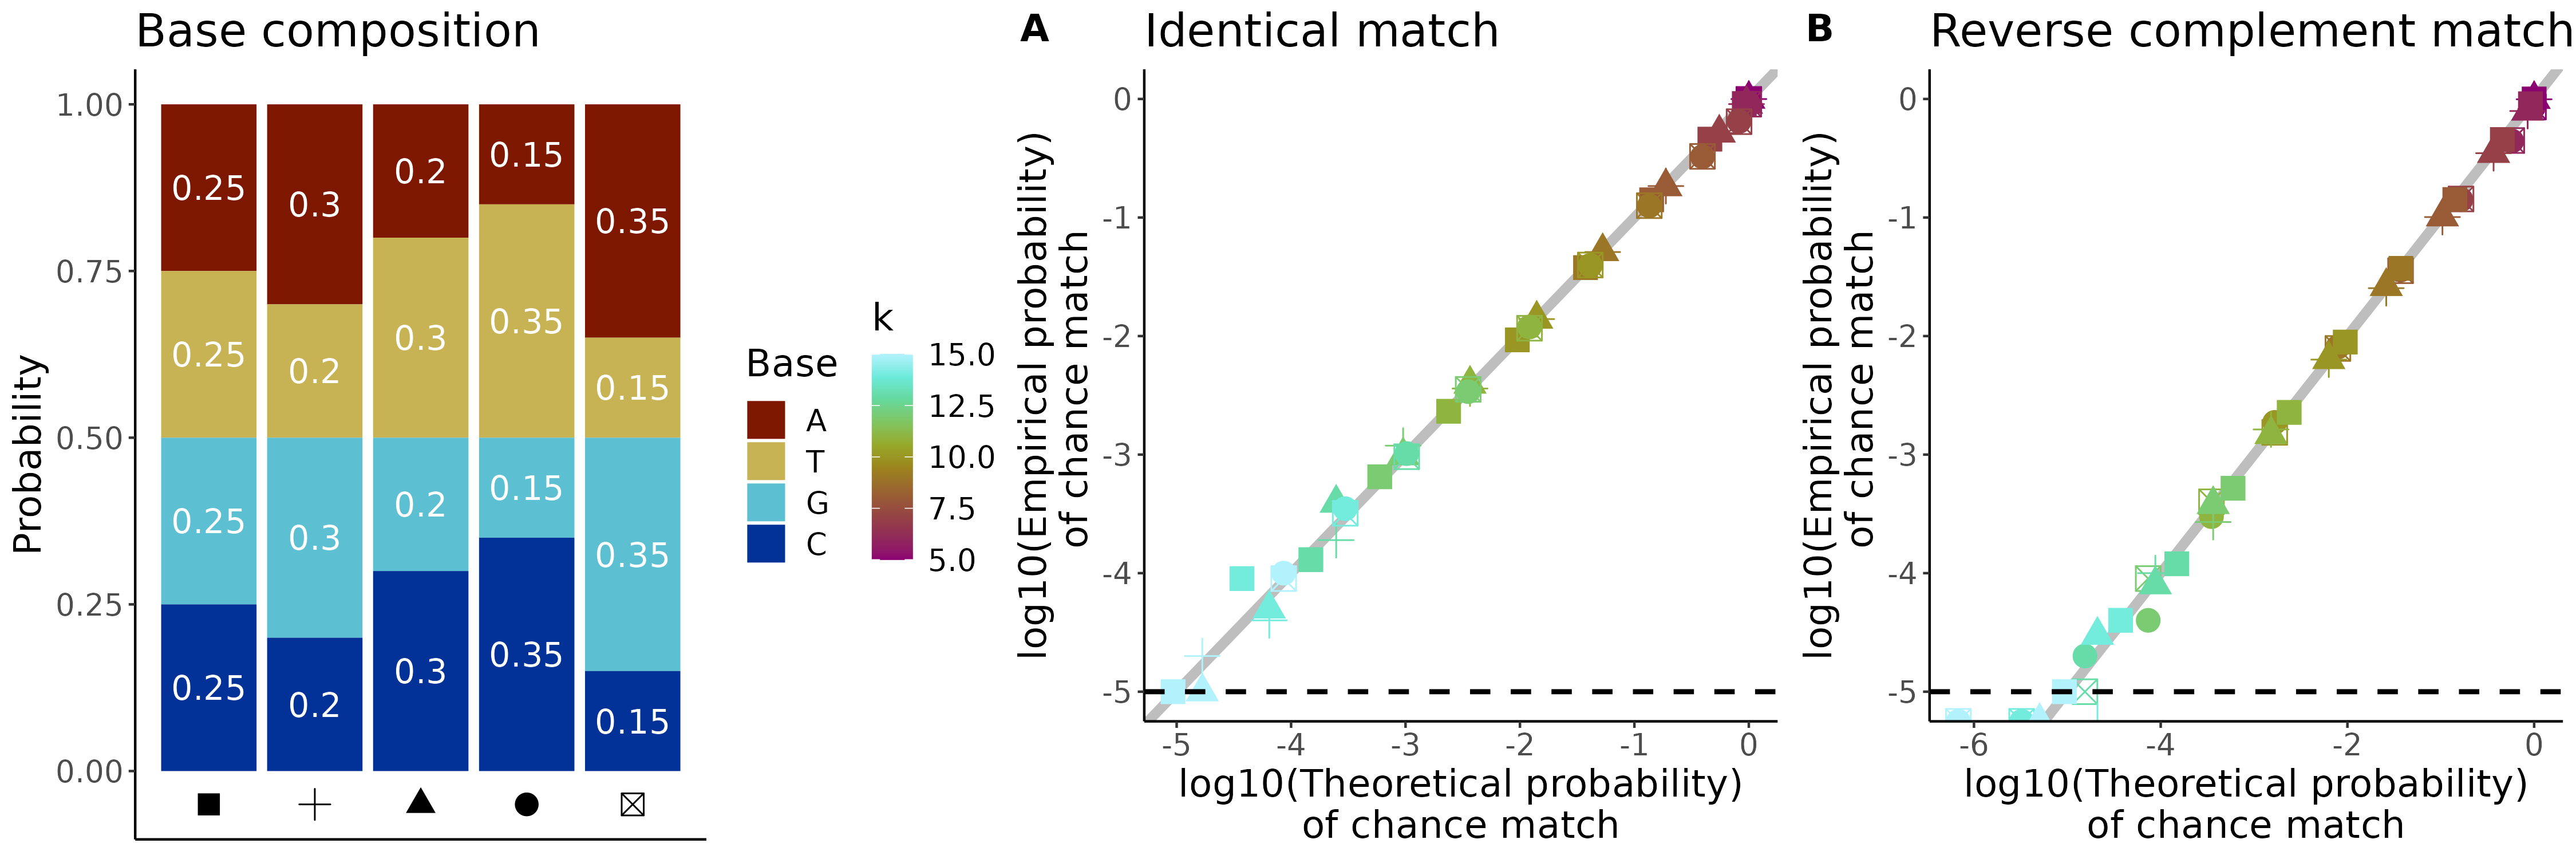
\includegraphics[width=\linewidth]{figures/chapter_3/kmer-review-sims-2024-12-06.png}
    \caption{\textbf{The relationship of $k$-mer length and base composition to chance matching.} We verified (A) Equation \ref{kfp_approx_f} and (B) Equation \ref{kfp_approx_r} by randomly generating 5.5 million pairs of k-mers and genomes. Each simulation had 100,000 trials. For each trial we randomly generated a genome of length 10,000 bases using a given base composition ($p_A$, $p_T$, $p_G$, $p_C$ in barchart) and also generated a random $k$-mer (color gradient shows $k$) using the same base composition. We then checked whether the random $k$-mer was in the random genome. In total, the 5 different base compositions $\times$ 11 different $k$-mer lengths $\times$ 100,000 trials per simulation gives 5.5 million trials total. Grey line is where the theoretical (i.e. Equations \ref{kfp_approx_f} and \ref{kfp_approx_r}) and empirical probabilities (i.e. from simulations) of a chance match are equal. Dotted black line shows the resolution of the simulations; because we did 100,000 trials per simulation we cannot empirically estimate probabilities smaller than 1/100,000.}
    \label{fig:equation-test}
\end{figure}

\subsection*{Choosing $k$ based on the balance of shared vs differing $k$-mers}

\begin{double}
    
A final class of approaches for choosing $k$ focuses on how if $k$ is small, most $k$-mers are shared between most samples, but as $k$ increases more sample-specific $k$-mers occur until no shared $k$-mers remain \citep{zhang_viral_2017}. Neither of these scenarios is usually desirable - the former makes all samples appear to be identical, while the latter makes all samples appear to be completely different. Thus, choosing $k$ boils down to balancing the number of shared vs differing $k$-mers. Some statistics for informing this choice include cumulative relative entropy \citep{sims_alignment-free_2009}, relative sequence divergence \citep{sims_alignment-free_2009}, average number of common features \citep{zhang_viral_2017}, Shannon's diversity index \citep{zhang_viral_2017}, and $\chi^2$ tests \citep{bai_optimal_2017}. However, there are two main drawbacks of these statistics. First, they were mainly developed for phylogenetic studies focused on short amino acid $k$-mers, so their utility for population genetics (which would probably focus on longer nucleotide $k$-mers) is untested. Furthermore, different values of $k$ will appear optimal for genomes of different sizes \citep{zhang_viral_2017}, making it hard to imagine that one optimal $k$ exists for a population exhibiting substantial genome size variation. Extending these or similar approaches to optimize $k$ for populations with genome size variation will be very useful for future studies.

\end{double}

\vspace{12pt}

\subsection*{Box 2: What's the expected value of $k$-mer diversity in a neutrally evolving population?}

\begin{double}
    
We argue that $k$-mers can be useful for initial assessments of genetic diversity, but two key questions are likely of interest to population geneticists: can $k$-mer diversity be related to nucleotide diversity (the common measure of genetic diversity) and what is the expected value of $k$-mer metrics for populations evolving under a given model? Here, we derive a simple bound on the expected number of $k$-mer differences between a pair of individuals in a neutrally evolving population. Our result is similar to \citep{shi_alignment-_2024}, except we generalize beyond haploid organisms.

We start by assuming that (1) $k$ is sufficiently long to capture all of the unique sequences in a genome, (2) each genome is sequenced at sufficient coverage to confidently identify all of the $k$-mers present, (3) $k$-mers are sequenced without error, and (4) only SNPs contribute to differences between genomes. Let $i$ and $j$ be individuals in a neutrally evolving population with ploidy level $x$ and let $y$ and $z$ be two haploid genomes in the pool of $i$ and $j$ that differ by origin. Next, let $K_i$ and $K_j$ represent the set of $k$-mers identified in individual $i$ and $j$'s genomes respectively and let $|K_i|$ denote the size of the set $K_i$. If all of the genomes within $i$ and $j$ are identical, then all $k$-mers are shared between them. If we start by assuming $i$ and $j$ are haploid, this means a maximum of $2k$ $k$-mers are not shared between $i$ and $j$ for every pairwise difference between $i$ and $j$ \citep{iqbal_novo_2012, younsi_using_2015}. This relationship can be written as:

\begin{equation} \label{eq:haploid_diff2k}
    |K_i \cup K_j| - |K_i \cap K_j| \leq 2kD_{yz}
\end{equation}

where $D_{yz}$ represents the number of pairwise differences between haplotypes $y$ and $z$ and the left side represents the number of $k$-mers exclusive to either $i$ or $j$. The reason for the using a ``$\leq$'' in Equation \ref{eq:haploid_diff2k} is to account for three possibilities: (1) if two SNPs are less than $k$ bases apart, there will be fewer than $4k$ $k$-mers not shared between $i$ and $j$, (2) it's possible for a SNP to turn one $k$-mer into a different $k$-mer that's already present elsewhere in a genome and (3) at higher ploidy levels, if a segregating site is heterozygous in $i$ and $j$ then $i$ and $j$ will share all $k$-mers between them.

To generalize beyond haploid organisms, we will replace the conversion factor of 2 in equation \ref{eq:haploid_diff2k} above with a general function $a(x)$:

\begin{equation} \label{eq:general_diff2k}
    |K_i \cup K_j| - |K_i \cap K_j| \leq a(x)\sum_{y<z}D_{yz}
\end{equation}

where $a(x)$ is a conversion factor that turns a number of pairwise differences into a number of sample-exclusive $k$-mers as a function of $x$ and $\sum_{y<z}D_{yz}$ is all of the pairwise differences for any pair of haplotypes $y$ and $z$ in $i$ and $j$. The values that maximize $a(x)$, maintaining the validity of using a ``$\leq$'' sign in Equation \ref{eq:general_diff2k}, are as follows:

\begin{equation}
      a(x)=\begin{cases}
    \frac{2k}{x^2}, & \text{if $1 \leq x \leq 3$}.\\
    \frac{k}{2x-1}, & \text{if $x \geq 4$}.
  \end{cases}
\end{equation}

When the population is haploid ($x = 1$), Equation \ref{eq:general_diff2k} reduces to Equation \ref{eq:haploid_diff2k}. When $x =$ 2 or 3, $a(x)$ is maximized when $i$ and $j$ are homozygous for different alleles, creating $2k$ sample-exclusive $k$-mers for every 4 or 9 pairwise differences, respectively. However, when $x \geq 4$, the situation that maximizes $a(x)$ is one where the SNP exists on only one haplotype in $i$ or $j$, creating $k$ sample-exclusive $k$-mers for every $2x-1$ pairwise differences.

Now we will convert the right side of Equation \ref{eq:general_diff2k} into nucleotide diversity ($\pi$). Summing across all pairs of individuals gives:

\begin{equation}
    \sum_{i<j}|K_i \cup K_j| - |K_i \cap K_j| \leq a(x)\sum_{i<j}\sum_{y<z}D_{yz}
\end{equation}

Next, we convert the right-hand side into genome-wide average $\pi$ by dividing both sides by the number of pairwise haplotype comparisons \citep{korunes_pixy_2021}, which is the number of individuals sampled $n$ times ploidy $x$, choose 2:

\begin{equation}
\frac{\sum_{i<j}|K_i \cup K_j| - |K_i \cap K_j|}{{nx\choose2}} \leq a(x) \left( \frac{\sum_{i<j}\sum_{y<z}D_{yz}}{{nx\choose2}}\right)
\end{equation}

\begin{equation}
    \frac{\sum_{i < j} |K_i \cup K_j| - |K_i \cap K_j|}{{nx\choose2}} \leq a(x)\pi
\end{equation}

Next, isolating $\pi$ on one side gives:

\begin{equation}\label{eq:ktopi}
    \frac{\sum_{i < j} |K_i \cup K_j| - |K_i \cap K_j|}{a(x){nx\choose2}} \leq \pi
\end{equation}

The intuition behind this formula is that, in a world where our assumptions are met, the number of $k$-mers that are not shared between a pair of samples is bounded by a multiple of $\pi$. The need to scale $\pi$ by $a(x)$ to get a bound reflects the fact that a given SNP can be captured by multiple $k$-mers, but the exact relationship between pairwise differences and sample-exclusive $k$-mers depends on ploidy.

Finally, we can substitute $\pi$ for the standard formula for the expected value of $\pi$ in a neutrally evolving population at equilibrium \citep{tajima_amount_1996}:

\begin{equation} \label{eq:expectedk}
    E \left[ \frac{\sum_{i < j} |K_i \cup K_j| - |K_i \cap K_j|}{a(x){nx\choose2}} \right] \leq \frac{2xN_e\mu}{1 + \frac{4}{3}2xN_e\mu}
\end{equation}

where $N_e$ is effective population size and $\mu$ is the mutation rate (probability of mutation per base pair per generation). The denominator on the right hand side of Equation \ref{eq:expectedk} ensures that the expected value of $\pi$ saturates as it approaches it's theoretical maximum of 0.75 \citep{tajima_amount_1996}. Altogether, equations \ref{eq:ktopi} and \ref{eq:expectedk} provide simple bounds for the average number of $k$-mers that differentiate a pair of samples in terms of $N_e$ and $\mu$.

\end{double}

\begin{figure}[H]
    \centering
    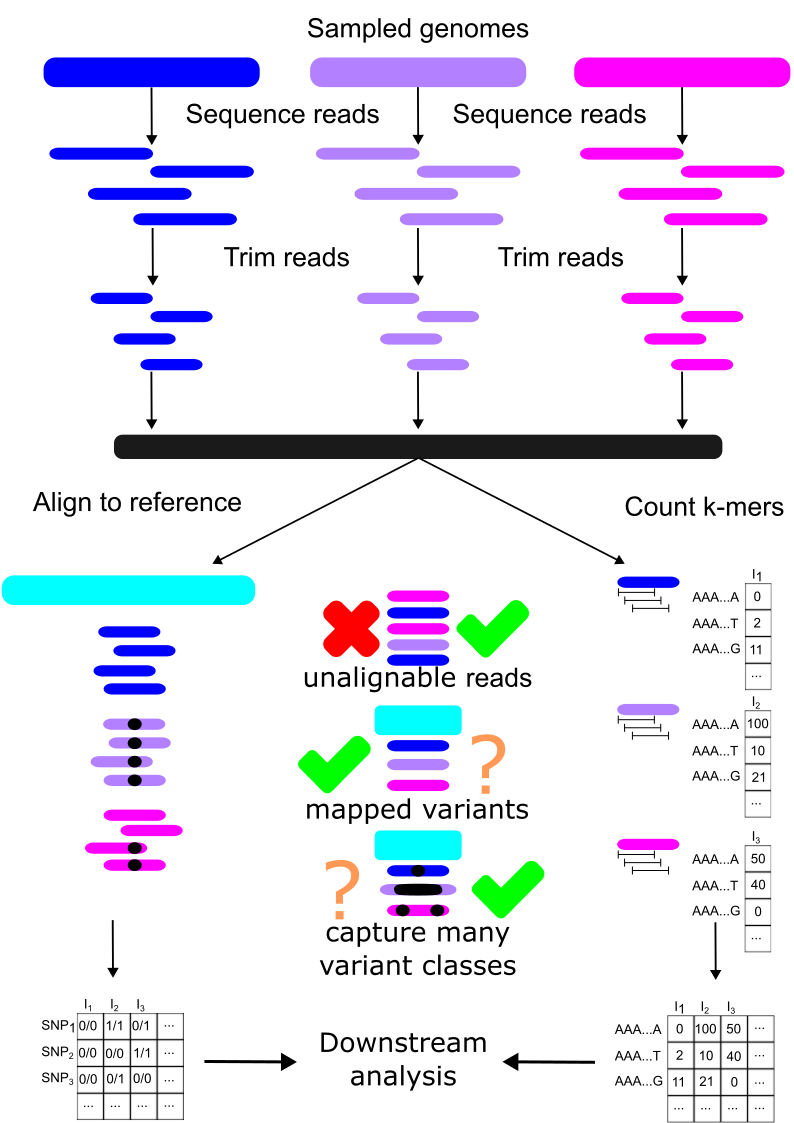
\includegraphics[width=0.7\textwidth]{figures/chapter_3/kmer_vs_snp_workflow.png}
    \caption{\textbf{Comparison between a typical SNP-calling workflow and a $k$-mer counting workflow.} A typical $k$-mer-based analysis begins the same as a SNP-based analysis: sequencing reads from sampled genomes followed by trimming and other quality control steps on the reads. The crucial difference comes down to whether the remaining reads are aligned to a reference sequence (discarding any unaligned reads) or are used for $k$-mer counting. Workflows may vary in terms of attempting to map $k$-mers to specific loci or calling variants other than SNPs (denoted with ``?''). The end result for each workflow is typically a matrix where each row is a different genomic variant, each column is a sample, and the elements represent the variant states. For SNPs, the standard variant call format notation is to use 0/0 to represent homozygous reference genotypes, 0/1 or 1/0 to represent heterozygous genotypes, and 1/1 to represent homozygous alternate genotypes. In $k$-mer based analyses the variant states are instead counts of how many $k$-mers of a particular type were observed in each sample.}
    \label{fig:kvs}
\end{figure}

\subsection*{Identifying variation with $k$-mers}
%\addcontentsline{toc}{subsubsection}{3.2: Identifying variation with \textit{k}-mers}

\begin{double}
    
Many of the earlier studies using $k$-mers to identify variants \textit{de novo} focus on microbes, where (despite small genome sizes) high levels of diversity make alignment and choosing a reference genome difficult \citep{gardner_scalable_2010}. However, similar approaches have now been extended to other taxa. One class of approaches calls SNPs \textit{de novo} simply by comparing $k$-mers between samples and searching for pairs of $k$-mers that differ at their central basepair \citep{gardner_scalable_2010, gardner_when_2013, bedo_information_2016, li_kmer2snp_2022}. Another, more popular, class of methods relies on de Bruijn graphs, which are graphs where $k$-mers are nodes and two nodes are connected if they share $k - 1$ bases \citep{compeau_why_2011}. SNPs in a sample then appear as ``bubbles'' in these graphs and calling SNPs amounts to searching for these bubbles \citep{iqbal_novo_2012, leggett_identifying_2013, younsi_using_2015, uricaru_reference-free_2015, standage_kevlar_2019, gauthier_discosnp-rad_2020}. Finally, other approaches first identify $k$-mers that are present in all samples (i.e. ``anchor'' $k$-mers) and finds paths between anchor $k$-mers through either local alignment or traversing de Bruijn graphs \citep{audano_mapping-free_2018, kaplinski_katk_2021, aylward_pankmer_2023}. The main drawback to these approaches is that the relative positions of the resulting variant calls are usually unknown without further analysis (see Figure \ref{fig:kvs}).

To call variants with known relative positions, it is possible to combine the strengths of $k$-mers with either pangenomes or databases of previously-identified variants. This is because unique variations in pangenomes will often be tagged by multiple unique $k$-mers. For example, one can compare $k$-mers with a reference set of SNPs  \citep{shajii_fast_2016, pajuste_fastgt_2017, denti_malva_2019, shi_identifying_2023, chu_ntsm_2024} or insertions \citep{puurand_alumine_2019} to quickly genotype samples without alignment. Or if a reference pangenome assembly is available, it's possible to use $k$-mers to infer the path through the pangenome corresponding to a given sample genome \citep{iqbal_novo_2012, ebler_pangenome-based_2022, grytten_kage_2022, hantze_effects_2023}. However, similar to common alignment-based SNP calling practices, the called variants will be limited to variants present in the pangenome reference.

If references are not already available, $k$-mers can be especially helpful for identifying and assessing variation in species with little prior knowledge. For example, the popular tools genomescope and smudgeplot use the distribution of $k$-mer counts in a sample (i.e. the $k$-mer frequency spectrum) to rapidly estimate important parameters, including genome size, heterozygosity, and ploidy structure all from unassembled read sets \citep{vurture_genomescope_2017, ranallo-benavidez_genomescope_2020}. $k$-mer frequency spectra can also identify unwanted variation that is potentially due to contamination (reviewed in \citet{cornet_contamination_2022}) or sequencing error. $k$-mers have the useful property that sequencing errors mainly manifest as $k$-mers that occur just once or a few times in a sample of reads \citep{kelley_quake_2010}. This is because random sequencing errors are unlikely to generate the same $k$-mer many times and (if $k$ is long enough, see Box 1) usually produce $k$-mers not found in the target genome. Thus, excluding low-copy $k$-mers from an analysis can mitigate sequencing error and one can examine the $k$-mer frequency spectrum to choose an appropriate $k$-mer count cutoff \citep{zhao_mining_2018}. Although $k$-mer frequency spectra can be usefully mined for genome parameters, their exact relationship to key population genetic parameters, such as measures of differentiation or diversity, remains underexplored.

\end{double}

\vspace{12pt}

\subsection*{Measuring variation with $k$-mers}
%\addcontentsline{toc}{subsubsection}{3.3: Measuring variation with \textit{k}-mers}

\begin{double}

After calling variants, quantifying levels of variation is a crucial step in many population genetics workflows. Because counting $k$-mers tends to be faster than alignment, $k$-mers could be especially helpful for rapid, initial assessments of diversity that complement or guide pangenome analysis. The standard approach to measure diversity in a population is to align sample sequences to a reference genome then calculate either (1) the average level of heterozygosity across sites or (2) the number of variants segregating in the sample. These are represented by Nei's (Equation \ref{eq:nei}; \citet{nei_mathematical_1979, nei_dna_1981}) and Watterson's (Equation \ref{eq:watterson}; \citet{watterson_number_1975}) estimators of diversity, respectively:

\begin{equation} \label{eq:nei}
    \pi = (1 - \sum_i p_{i}^{2})(\frac{n}{n - 1})
\end{equation}

\begin{equation} \label{eq:watterson}
    \theta_w = \frac{S}{\sum_{a = 1}^{a = n-1}\frac{1}{a}}
\end{equation}

where $n$ is the number of sequences in the sample, $p_i$ is the frequency of the $i$th allele at a locus, and $S$ is the number of segregating sites at a locus. While $\theta_w$ is based on a discrete count of variants ($S$), $\pi$ is shaped by the allele frequencies of variants and will be higher if variants are common than if variants are rare (note that $\pi$ is more commonly rewritten in terms of the average number of differences between sequences \citep{korunes_pixy_2021}). 

Can analogous measures of variation be derived from $k$-mers? There are over 30 valid measures of genetic difference based on $k$-mer counts used in previous literature \citep{benoit_multiple_2016, zielezinski_alignment-free_2017, luczak_survey_2019, zielezinski_benchmarking_2019}. However, the three most common $k$-mer dissimilarity measures are arguably Jaccard dissimilarity (Equation \ref{eq:jaccard}; \citet{ondov_mash_2016}), Bray-Curtis dissimilarity (Equation \ref{eq:bray}; \citet{dubinkina_assessment_2016, benoit_simkamin_2020}), and cosine dissimilarity (Equation \ref{eq:cos}, \citet{choi_libra_2019}):

\begin{equation} \label{eq:jaccard}
    J(K_i,K_j) = 1 - \frac{K_i \cap K_j}{K_i \cup K_j}
\end{equation}

\begin{equation} \label{eq:bray}
    B(C_i,C_j) = 1 - 2\sum^{4^k}_{b = 1}\frac{\min(m_b(C_i), m_b(C_j)) }{m_b(C_i) + m_b(C_j)}
\end{equation}

\begin{equation} \label{eq:cos}
    C(C_i,C_j) = 1 - \frac{C_i \cdot C_j}{\|C_i\| \times \|C_j\|}
\end{equation}
where $k$ is the length of $k$-mers to be included in the comparison, $K_i$ and $K_j$ are the set of $k$-mers of length $k$ present in a set of reads $i$ and $j$, $C_i$ and $C_j$ are vectors of $k$-mer counts in a set of reads $i$ and $j$, and $m_i$ is a function that returns the relative frequency of the $b$th $k$-mer in a set (i.e. standardized such that $\sum^{4^k}_{b = 1} m_b(C_i)$ and $\sum^{4^k}_{b = 1} m_b(C_j)$ equal 1). These measures work similarly to the classical $\pi$ and $\theta_w$ measures: the numerators are a measure of the number of sites that vary between individuals, while the denominators are a measure of sample size (here the number of $k$-mers rather than number of haplotypes). The main difference, however, is that $k$-mer-based measures of genetic dissimilarity are not directly interpretable in terms of mutations, like $\pi$ and $\theta_w$ can be with the assumption that each SNP represents one mutation \citep{Haubold_alignment-free_2011, Haubold_alignment-free_2012}. Any given $k$-mer may represent the combined presence of multiple mutations \citep{voichek_identifying_2020,blanca_statistics_2022} and any mutation can generate multiple new $k$-mers. Although this means that $k$-mer-based genetic dissimilarity measures are only proxies for the true mutational distance between individuals, they still effectively resolve relationships between lineages compared to alignment-based measures \citep{vanwallendael_alignment-free_2022}.

While Equations \ref{eq:jaccard}, \ref{eq:bray}, \ref{eq:cos} have all been successfully used to measure genetic dissimilarity between samples in past studies, the formulae highlight their benefits and drawbacks. First, Jaccard dissimilarity, perhaps the most commonly used $k$-mer dissimilarity metric \citep{ondov_mash_2016, ruperao_exploring_2023}, requires only knowing $k$-mer presence/absence patterns in samples instead of $k$-mer counts and thus can take less memory to calculate than other $k$-mer-based dissimilarity measures. However, as a consequence Jaccard dissimilarity may not capture the effects of copy number variation and does not account for variation in coverage between samples, which affects whether a given $k$-mer is called as ``present'' in a sample \citep{vanwallendael_alignment-free_2022}. Approaches that measure $k$-mer counts, like Bray-Curtis dissimilarity (Equation \ref{eq:bray}) and cosine dissimilarity (Equation \ref{eq:cos}), can better account for these influences, but may require more memory for storing counts \citep{liu_unbiased_2017, choi_libra_2019}. To alleviate this memory problem, many approaches calculate approximate $k$-mer dissimilarity measures with a small subset of $k$-mers \citep{ondov_mash_2016, zhao_bindash_2019, benoit_simkamin_2020, Pellegrina_fast_2020}. An alternative approach would be to instead compress the $k$-mer counts into a smaller array, keeping information from more $k$-mers while simultaneously alleviating memory burdens \citep{melsted_efficient_2011}, but such approaches have not been used to calculate genetic dissimilarity before. The relationship between $k$-mer-based dissimilarity measures and $\pi$ is also rarely explored. While some studies have investigated the relationship between $\pi$ and Jaccard dissimilarity \citep{vanwallendael_alignment-free_2022}, other $k$-mer dissimilarity measures are possible and no studies to our knowledge have compared these approaches for populations of varying levels of diversity - a key determinant of whether alignment-based genotype calls are accurate \citep{cornish_comparison_2015, bush_genomic_2020}. In the following sections, we investigate the efficacy of compressed and uncompressed $k$-mer-based measures of variation at capturing the true pairwise diversity of simulated populations.

\end{double}

\vspace{12pt}

\subsection*{Testing the efficacy of $k$-mer measures of variation.}

\begin{double}
    
We used simulations to investigate the relationship between the true value of $\pi$ and genetic diversity measured from $k$-mer based approaches from simulated sequencing reads. 

\end{double}

\vspace{12pt}

\subsubsection*{Simulations}

\begin{double}

We simulated a neutrally evolving 100kb segment of the \textit{Arabidopsis thaliana} genome. We first forward simulated 300 neutrally evolving populations with SLiM 3 \citep{haller_slim_2019}. Each population consisted of 100 individuals simulated for 1000 generations with a uniform recombination rate of $10^{-8}$. To vary the diversity across simulations we varied the mutation rate between $10^{-6}$ and $2*10^{-4}$. For each simulation, we tracked the ancestry through tree-sequence recording which records the geneological history of all samples \citep{slimTreeRecording}. From these trees, we generated sequences based on the \textit{Arabidopsis thaliana} genome (chromosome 1 at positions 4,185,001-4,285,000) \citep{Kent2002-xv}. We took a sub-sample of 10 individuals from the tips of the trees and randomly assigned nucleotides to each SNP in the sample using msprime version 1.2.0 and tskit version 0.5.6 \citep{baumdicker2022efficient}. From the sub-tree of the sampled genomes, we recorded the exact number of true average pair-wise differences ($\pi_t$) across the sample of 10 individuals (20 chromosomes) using msprime \citep{baumdicker2022efficient}. 

\end{double}

\vspace{12pt}

\subsubsection*{Generating $k$-mers}

\begin{double}

To test the performance of the $k$-mer measures on unaligned reads, we simulated reads for each genome using an Illumina read simulator, InSilicoSeq 2.0.0 \citep{gourle_simulating_2019}. We varied the read count to later investigate the effect of coverage as described below. We generated two sets of reads for each individual at coverages of 10x and 30x. After simulating reads, we counted $k$-mers within the reads using KMC3 \citep{deorowicz_kmc_2015, kokot_kmc_2017}. We generated $k$-mer count vectors with $k=10, 20, 30,$ and $40$ for each individual. We used a threshold-based approach to adjust the $k$-mer vectors to reduce the effects of sequencing errors; any $k$-mer count below the threshold value was set to zero for a particular sample before any dissimilarity calculations. For a threshold of 5, only $k$-mers with counts of 5 or more were considered when calculating the difference between two or more groups of $k$-mer counts. We present data with a threshold of 5, but note that a threshold of 0 is qualitatively similar with dissimilarity scores being slightly higher overall. This practice of filtering out low-coverage $k$-mers is analogous to the common practice of filtering out SNPs below a given minor allele frequency threshold \citep{asif_gwas_2021}. After $k$-mer counting, we calculated the genetic dissimilarity of populations with the Bray-Curtis (Equation \ref{eq:bray}) and cosine dissimilarity (Equation \ref{eq:cos}) measures.

\end{double}

\vspace{12pt}

\subsubsection*{The effect of $k$ on $k$-mer similarity metrics}

\begin{figure}[H]
  \centering
  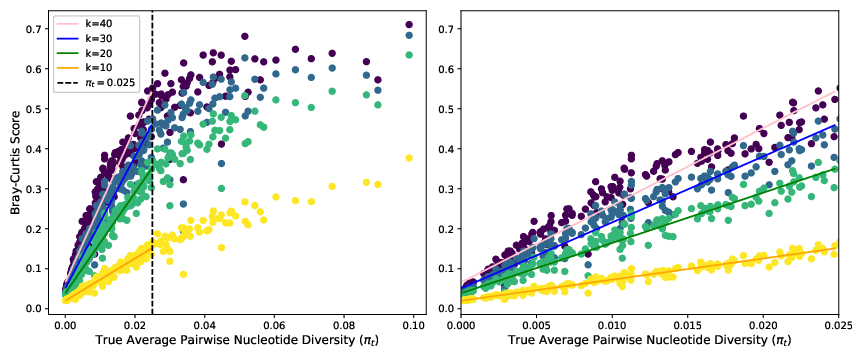
\includegraphics[width=\linewidth]{figures/chapter_3/bray_curtis_30x.png}
  \caption{\textbf{Effect of $k$ on Bray-Curtis dissimilarity.} Bray-Curtis dissimilarity calculated from simulated reads with a coverage of 30 where each point represents a sample of 20 chromosomes. Displayed are 10-mers (yellow), 20-mers (green), 30-mers (blue), and 40-mers (purple) each with a linear regression line for $\pi_t$ between 0 and 0.025. The scores for populations with a $\pi_t$ less than 0.025 is shown to the right.}
  \label{fig:BCCov30Kmers}
\end{figure}

\begin{double}

Figure \ref{fig:BCCov30Kmers} shows the effect of $k$ on the Bray-Curtis score with 30x coverage. We observe a plateau in the scores when diversity exceeds $\pi\approx2.5\%$. This plateau occurs because, when diversity is high, SNPs cause most of the $k$-mers to be different between two samples. This effect is especially true with high $k$ values as one variant sampled in only one read can appear in up to $2k$ $k$-mers if it is sampled away from the edges of a read. The elevated number of $k$-mers at high diversity means that it is harder to interpret differences in dissimilarity measures between samples above this threshold, but this problem can be mitigated by using a lower $k$ value, such as $k$=10 when the expected diversity in a sample is high. If $\pi_t$ is expected to be below 0.025, larger $k$ values can have higher precision and capture more unique $k$-mers in individual samples, better estimating true diversity.

While the data presented in Figure \ref{fig:BCCov30Kmers} were simulated with a coverage of 30x, Figure D1 shows that a coverage of 10x results in qualitatively similar scores when $k$=30. While coverage affects the precision of the measures, the overall trends and relative rankings between simulations remain consistent. 

\end{double}

\begin{figure}[H]
  \centering
  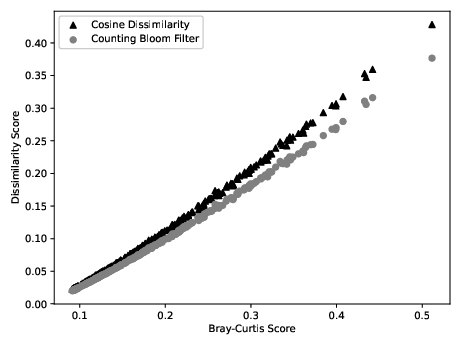
\includegraphics[width=.8\linewidth]{figures/chapter_3/direct_kmer_score_comparison.png}
  \caption{\textbf{Effect of bloom filter on cosine dissimilarity.} Cosine dissimilarity (triangle) and counting bloom filter scores (circle) from 10-mers of simulated reads with a coverage 30 compared directly against the Bray-Curtis score of each simulated set of 10 individuals (points).}
  \label{fig:AllThree}
\end{figure}

\subsubsection*{The Counting Bloom filter approach to comparing genomes}

\begin{double}

Bloom filters are a data structure that can compress a $k$-mer count vector into a smaller array \citep{melsted_efficient_2011}. We can compute the dissimilarity of two compressed vectors using less memory and with increased efficiency as fewer entries are compared. Counting bloom filters (CBFs) are modifications of bloom filters \citep{fan2000summarycache}, and are used in alternative $k$-mer count methods and error correction in sequencing data \citep{melsted_efficient_2011, roy2014turtle, shi2010quality}. CBFs compress the $k$-mer vectors through several hash functions that map to a smaller array. Counting bloom filters will increase the $k$-mer count in the position as opposed to setting the count to one if a $k$-mer has been mapped there (see Figure \ref{fig:CBFDiagram}). Because of the hash-functions and collisions, false positives are possible; here a ``false positive'' means that two $k$-mers of different sequences may map to the same locations in the vector (i.e. have a hash collision). However, identical mapping of two different $k$-mers is not a concern for relative comparison of diversity, since the same hash functions are used for each sample so collisions are consistent across samples. Collisions will cause diversity to be underestimated, but we can reduce collisions by increasing the number of hash-functions used in the process \citep{melsted_efficient_2011}.

A CBF gives a standardized way to compare across species/experiments if the vectors for $k$-mer counts are set to the same size and the same hash functions are used to generate the vectors across data sets. We can also perform the same cosine dissimilarity measure on the CBF vector that we use directly on the counts of $k$-mers. The cosine dissimilarity measure on the raw $k$-mer count vectors has the same $R^2$ to the compressed CBF vectors ($0.97$) when comparing the scores to $\pi_t$. Figure \ref{fig:AllThree} shows that the cosine dissimilarity using the counting bloom filter is qualitatively similar to the cosine dissimilarity with the raw $k$-mer counts. This similarity and the high $R^2$ mean that the predictability of $\pi_t$ is maintained while using the smaller, more manageable CBF data structure. Therefore, we can reliably use the CBF data structure as opposed to the raw $k$-mer counts to calculate the cosine dissimilarity of two samples.

The memory usage of a $k$-mers vector for a sample with 10x coverage and $k=30$ under our simulations is around 4.5 MB per sample. The memory usage is reduced to 0.02 MB when compressed to a 10,000 element array of unsigned 16-bit integers. Therefore, storing and using $k$-mer counts for measuring diversity scale much better under the CBF data structure.

\end{double}

\begin{center}
\begin{figure}[H]
  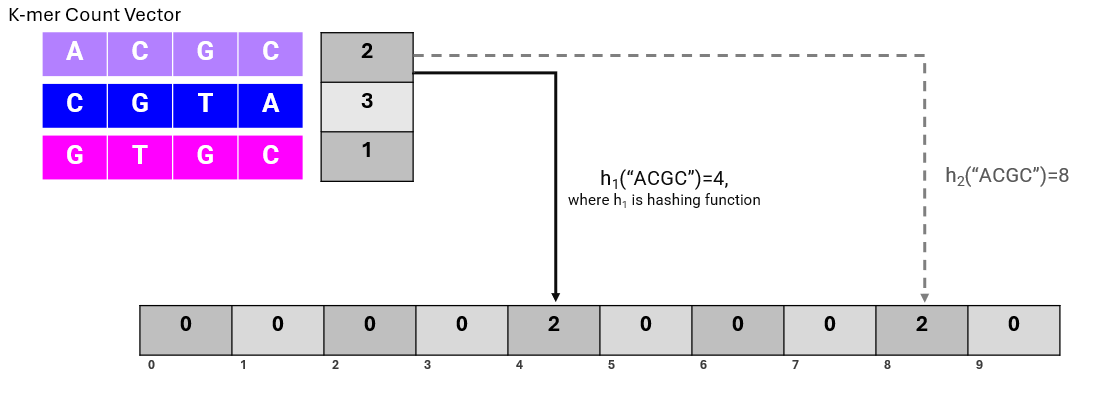
\includegraphics[width=\linewidth]{figures/chapter_3/cbf_schematic.PNG}
  \caption{\textbf{A conceptual schematic of a Counting Bloom Filter.} When the first 4-mer, ``ACGC", is hashed, the hash function $h_1$ outputs 4 and $h_2$ outputs 8. Both positions in the CBF array are incremented by 2 as that is the count of ‘ACGC’ in the given $k$-mer count vector.}
  \label{fig:CBFDiagram}
\end{figure}
\end{center}

\subsubsection*{The effect of array size on CBF measures of diversity}

\begin{double}

We found that the size of the CBF array scales the cosine dissimilarity score and keeps the rank of scores very similar as the array size changes. Since rank is maintained, we can take advantage of much smaller arrays without losing much information about the relative diversity scores between samples. Smaller arrays allow for less memory usage, and faster computing of cosine dissimilarity. Supplementary Figure D2 compares the scores of a CBF array of size 20 million and 10 thousand on the same simulations. We observe that the smaller array adjusts the scores down while maintaining the same rank of scores. For example, these results show that if a population has the lowest cosine score with the 20 million length array, it remains among the lowest scores with a 10 thousand length array. This result means that it may be possible to adjust the vector size 
 such that the cosine dissimilarity scores are similar in magnitude and scale to the true pairwise nucleotide diversity which can be useful for prediction of the score without alignment, and can make interpretation simpler. However, the viability of this approach still needs to be investigated across different species and genomic contexts, it is likely there is not a `one size fits all' array size that would scale cosine dissimilarity to match $\pi$ universally. Our simulations only consider SNPs, neutral evolution, and the \textit{Arabidopsis thaliana} genome. It is still left to determine the effects of other mutations types such as insertions, deletions, and inversions as well as other evolution types. Therefore we should avoid the potential pitfalls of interpreting a scaled value directly as $\pi$ unless future work shows that to be appropriate. 

\end{double}

\vspace{12pt}

\subsection*{Explaining variation with $k$-mers}
%\addcontentsline{toc}{subsubsection}{3.4: Explaining variation with \textit{k}-mers}

\begin{double}

A common first step to understanding the evolutionary forces shaping variation in populations involves quantifying differentiation between populations. Patterns of differentiation in SNP genotypes are often summarized and plotted using dimension reduction techniques, such as principal component analysis (PCA) \citep{novembre_interpreting_2008}. $k$-mer genotypes are also amenable to PCA and recover the same differentiation patterns as SNP-based PCA \citep{liu_unbiased_2017, murray_kwip_2017, rahman_association_2018, ho_intraspecific_2019, hrytsenko_determining_2022}. Applying dimensional reduction to $k$-mers can even differentiate species \citep{rosen_metagenome_2008, aflitos_cnidaria_2015, bernard_recapitulating_2016, linard_rapid_2019, bodde_high-resolution_2022}, something that can be difficult to do with SNPs without multiple sequence alignment. Interestingly, $k$-mers from repetitive sequences may not always differentiate populations that are clearly differentiated in terms of their SNP genotypes \citep{renny-byfield_repetitive_2020}, suggesting that identifying the set of $k$-mers that best differentiate populations could be an important avenue for future research. Furthermore, while we are aware of one study in yeast that estimates admixture proportions from $k$-mers \citep{shi_alignment-_2024}, more investigation is needed to see if this approach works for other species.

Besides polymorphism between populations, $k$-mers are also useful for explaining polymorphism patterns across genomes in terms of specific evolutionary forces. For instance, the $k$-mer profile of a given locus is often predictive of the local recombination rate \citep{liu_sequence-dependent_2012, Haubold_alignment-free_2013, Haubold_alignment-free_2014, frenkel_organizational_2016, al_maruf_irspot-sf_2019} and the local mutation rate \citep{aggarwala_expanded_2016, carlson_extremely_2018, bethune_method_2022, adams_regularized_2023, beichman_evolution_2023, liu_structural_2023}. $k$-mers can capture information about recombination and mutation because these processes often associate with specific functional DNA motifs \citep{myers_common_2008, ruzicka_dna_2017}. However, $k$-mers are also intrinsically sensitive to sequence changes and while there are some existing methods to identify new mutations \citep{nordstrom_mutation_2013, ho_intraspecific_2019} and sites of recombination \citep{Fletcher_AFLAP_2021} solely from $k$-mers, further development is needed. Being able to predict fine scale variation in mutation and recombination rates solely from the $k$-mer profile of a reference sequence would be extremely beneficial because these processes frequently confound scans for sites of selection \citep{huber_detecting_2016}. However, this would require further study of the relationship between $k$-mers and mutation/recombination rates across wider ranges of species.

$k$-mers also offer opportunities to explore patterns of selection. One general assumption in $k$-mer literature is if a $k$-mer is shared across all individuals of a population or species then it is potentially under selection to be conserved \citep{bernard_recapitulating_2016, aylward_pankmer_2023}. In contrast, a $k$-mer that is not present in any individual is possibly selected against (although this assumes that $k$ is sufficiently small such that the total possible $k$-mer space is small, as might be true when analysing small amino acid-derived $k$-mers)  \citep{Georgakopoulos-Soares_absent_2021}. However, it is unlikely that selection is solely responsible for patterns of $k$-mer sharing across individuals or species, so more rigorous approaches are needed. One potentially more rigorous approach would be to investigate $k$-mers that differentiate populations as candidates for loci underlying local adaptation, similar to $F_{ST}$ \citep{kane_selective_2007}. Although, we are not aware of any papers that employ this specific approach, identifying group-specific $k$-mers is a very common and useful practice, with one example being the assembly of sex-specific sequences \citep{Akagi_y-chromosomeencoded_2014, Ou_ngs-based_2017, Liao_genomic_2020, Neves_male_2020, mehrab_efficient_2021, wu_inferring_2021, Behrens_sex_2022, Fong_evolutionary_2023, Lichilin_no_2023}. There are some metrics of $k$-mer differentiation in published literature already \citep{rahman_association_2018}, but they do not have the same interpretation as $F_{ST}$. An alternative approach would be to march through a deBruijn graph \citep{aylward_pankmer_2023} to find strings of $k$-mers with selective sweep-like patterns, mainly low diversity, high linkage disequilibrium between $k$-mers, an excess of rare $k$-mers \citep{alachiotis_raisd_2018}, high differentiation between populations \citep{zhong_hard_2022}, and high haplotype homozygosity \citep{klassmann_detecting_2022} which could be determined based on $k$-mer copy number \citep{vurture_genomescope_2017,ranallo-benavidez_genomescope_2020}.  

There are only a few model-oriented studies that compare the $k$-mer spectrum observed in a genome to a neutral expectation, mostly in the context of detecting selection on transcription factor binding motifs \citep{gerland_selection_2002, ke_positive_2008, raijman_evolution_2008, yeang_quantifying_2010, gyorgy_competition_2023}. The basic idea behind these approaches is to first derive a neutral substitution model - which describes the probability of one nucleotide being substituted for another in a neutrally evolving sequence \citep{ke_positive_2008, raijman_evolution_2008} - then measure deviations from that neutral model according to the presence/absence of particular $k$-mers in a genome. Although these models are able to detect selection on $k$-mers that exist in multiple places across a genome, as is the case with binding motifs, it is unclear whether they could be applied to $k$-mers that represent unique genomic sequences. 

\end{double}

\vspace{12pt}

\subsection*{Challenges in investigating $k$-mers} 

\begin{double}

Despite the wide potential of $k$-mers to be useful for population genetic studies, there are three important limitations to keep in mind for most $k$-mer investigations. First, interpreting the biology of specific $k$-mers is often a challenge. One option is to take the candidate $k$-mers identified from an analysis and either align the $k$-mers themselves, the reads containing said $k$-mers, or assembled reads containing said $k$-mers to a reference genome \citep{voichek_identifying_2020} or a database of known sequences and motifs. While this is effective at pinpointing concrete type of variants at play in a system, it partially defeats the purpose of using $k$-mers in the first place because $k$-mers of interest may not be present in a reference genome. Second, since each sequencing error can generate up to $k$ erroneous $k$-mers and general practice is to discard reads with many unique $k$-mers to reduce the effect of error rates \citep{zimin_masurca_2013}, analysis of $k$-mers typically requires datasets with high coverage ($>$10x) and low sequencing error rates. These criteria can potentially exclude long-read datasets \citep{vurture_genomescope_2017} or reduced-representation datasets where genomes are sequenced at lower coverage to cut costs. Approaches that apply $k$-mers in lower coverage or higher error-rate datasets are needed. Third, $k$-mer-based analyses can frequently involve hundreds of millions or billions of unique $k$-mers. Storing and processing this many $k$-mers at once is often not feasible even on high performance computing systems. Two approaches to solving this issue are to subset one's $k$-mers \citep{ondov_mash_2016, benoit_simkamin_2020, zhao_bindash_2019, yi_kssd_2021}, or, as we discuss here, compress vectors of $k$-mer counts into an array of smaller size \citep{melsted_efficient_2011}. However, these solutions are usually developed for specific contexts, such as measuring genomic dissimilarity, and may not be applicable to every population genetic analysis. Future studies need to carefully consider common approaches to decreasing the disk burden of $k$-mer-based analyses and should explore new potential solutions. 

These challenges to studying $k$-mers highlight how $k$-mer based methods should be viewed as complementary to, instead of better than, pangenomes in many situations. Among other benefits, pangenomes have ready biological interpretations and provide greater information on linkage between sequences. However, the fact that $k$-mers can be studied with fewer computing resources and simpler sequencing data sets makes them potentially useful for either preliminary pangenomic analyses or situations where constructing many reference quality genomes is not yet feasible. 

\end{double}

\vspace{12pt}

\subsection*{Conclusions}
%\addcontentsline{toc}{subsubsection}{3.5: Conclusions}

\begin{double}

Current literature demonstrates that $k$-mers are useful for identifying, measuring, and explaining variation within populations without performing alignment. Through our own simulations of neutrally evolving populations, we find that $k$-mer dissimilarity reliably scales with nucleotide diversity and $k$-mer matrices can be compressed with minimal loss of dissimilarity information. However, further development is needed to make $k$-mers amenable to a wider array of population genetic tasks, especially the identification of selected loci and population structure. Further developing alignment-free approaches to population genetics tasks will ultimately help guide and complement the analysis of pangenomes.

\end{double}

\vspace{12pt}

\subsection*{Future directions}

\begin{double}

\begin{myitemize}
    \item Can we develop criteria for choosing values of $k$ that account for population-level variation in genome size or genome content?
    \item Can we develop $k$-mer-based estimates of population differentiation that are more similar to $F_{ST}$?
    \item Can we identify putative selective sweeps using $k$-mers?
    \item Can we develop applications of $k$-mers that are amenable to lower-coverage or pooled sequencing samples that are common in population genetics?
    \item $k$-mers are useful for getting preliminary estimates of important genome parameters that are useful for tuning pangenome assembly \citep{ranallo-benavidez_genomescope_2020}. What other types of preliminary pangenome analyses might $k$-mers be useful for?
    \item Can $k$-mers, either in combination with or without a pangenome reference, be useful for rapidly estimating allele frequencies and performing demographic inference?
\end{myitemize}

\end{double}

\vspace{12pt}

\subsection*{Data availability}

\begin{double}
    
Supplemental figures can be found in Appendix D. Scripts for simulation and data analysis can be found at: \url{https://github.com/williarj/kmers2024}.

\end{double}

\newpage

\section*{CHAPTER 4: SUMMARY STATISTICS COMPARABLE TO CONVOLUTIONAL NEURAL NETWORKS FOR INFERRING TIMES TO FIXATION\footnote{At the time of writing, this chapter is unpublished.}}
\addcontentsline{toc}{subsection}{CHAPTER 4: SUMMARY STATISTICS COMPARABLE TO CONVOLUTIONAL NEURAL NETWORKS FOR INFERRING TIMES TO FIXATION}

\setcounter{figure}{0}
\renewcommand{\figurename}{Figure}
\renewcommand{\thefigure}{4.\arabic{figure}}

\setcounter{table}{0}
\renewcommand{\tablename}{Table} 
\renewcommand{\thetable}{4.\arabic{table}}

\setcounter{equation}{0}
\renewcommand{\theequation}{4.\arabic{equation}}

\vspace{12pt}

\subsection*{Abstract}

\begin{double}
    
Times to fixation ($t_f$) are an essential ingredient for understanding neutral theory and positive selection. However, studies of $t_f$ have largely subsided in recent years and few methods exist to predict the time to fixation for a fixed beneficial allele. A key difficulty in this prediction problem is disentangling $t_f$ from the age of a sweep ($t_a$) because multiple different combinations of $t_f$ and $t_a$ can result in similar polymorphism patterns around the site of the sweep. We test whether convolutional neural networks (CNNs) can potentially perform better on this problem by simulating approximately 250,000 selective sweeps across five different demographic scenarios. The CNNs achieve comparable performance to  approximate bayesian compuation methods used in previous approaches. The CNNs are better able to disentangle $t_f$ from $t_a$ for populations that are growing, but also give statistically worse predictions than ABC when trained on populations cycling between two different sizes. Altogether this suggests that perhaps few undiscovered signals remain in single timepoint unphased genotype data that can be used to disentangle $t_f$ and $t_a$ in singe population demographic scenarios.

\end{double}

\vspace{12pt}

\subsection*{Introduction}
%\addcontentsline{toc}{subsubsection}{4.1: Introduction}

\begin{double}

%Anchor articles:
%\begin{itemize}
%    \item \citep{cecil_convolutional_2023}
%    \item \citep{ormond_inferring_2016}
%    \item \citep{kern_diploshic_2018} - assumed that fixation occurred immediately prior to sampling?
%\end{itemize}

Adaptation requires increasing the frequency of beneficial alleles in a population, but these frequency changes take time. How long does it take for beneficial alleles to spread? This question was at the top of mind of naturalists in the early 20th century as there was doubt over how reasonable natural selection was as an evolutionary mechanism (see \citet{charlesworth_how_2020} for a fuller historical treatment). The thinking was that if beneficial alleles change frequency only very slowly, then maybe natural selection is not important. However, early models outlined how selection can rapidly change allele frequencies, though most beneficial alleles are lost by drift \citet{fisher_xxidominance_1923, haldane_mathematical_1927}. Nonetheless the rate of new mutations is high enough such that new beneficial alleles are continually introduced and some eventually fix \citep{zhao_characteristic_2013}. As it became appreciated that multiple fixations can build up between species, further investigations of fixation times were motivated by observations of molecular substitution rates \citep{kimura_average_1969} and trait degradation as a result of relaxed selection \citep{kimura_average_1980}. The theories from this foundational work have since been extended to understand how time to fixation is shaped by changing environments \citep{cui_fixation_2018, kaushik_time_2021} and population structure \citep{greven_fixation_2016}. 

However, despite this foundation of knowledge, studies of times to fixation have subsided in recent years such that two different papers spaced 8 years apart both argue that times to fixation need more attention from modern methods \citep{zhao_characteristic_2013, charlesworth_how_2020}. It is much more common for studies to estimate coalescence times \citep{y_c_brandt_evaluation_2022}, variant age \citep{bisschop_sweeps_2021}, or allele frequency trajectories of currently segregating alleles \citep{stern_approximate_2019}. One reason for this focus is that coalescent times are foundational to important population genetic structures like ancestral-recombination graphs \citep{lewanski_era_2024}. Another reason is because $t_f$, in a simple model of a single additive \textit{de novo} beneficial mutation, is tightly correlated to the selection coefficient. The mean time to fixation for a single additive beneficial mutation in a constant sized population is $2ln(2cN_e-1)/s$ where $c$ is ploidy level \citep{otto_fixation_2013}. This equation is sensitive to $s$ more than $N_e$ because $s$ is outside of the logarithm. Thus, under this model one could study the selection coefficient and get essentially the same information as would be provided by $t_f$. However, the exact relationship between time to fixation and $s$ is more complicated when arbitrary dominance, mating system variation, and demographic changes are considered \citep{glemin_extinction_2012}. Selection coefficients and coalescent times thus do not fully convey the timescale of fixation by themselves outside of simple scenarios. 

How can we estimate $t_f$? Assuming a single \textit{de novo} additive mutation that is sampled immediately after sweep completion, there are simple models describing how the dip in diversity around a selected site varies with $t_f$ \citep{coop_population_2020}. There are more complex models requiring different sets of assumptions \citep{he_estimation_2020, bisschop_sweeps_2021}; however, not all study systems and situations will appropriately fit the assumptions in these models. As a result, there are several methods that forgo explicit models and instead simulate sweeps and use approximate bayesian computation (ABC) to estimate the timing of selection \citep{przeworski_estimating_2003, ormond_inferring_2016, nakagome_inferring_2019}. Machine learning algorithms can also be trained on simulations and have proven useful for a variety of population genetics tasks \citep{kern_diploshic_2018, flagel_unreasonable_2019, torada_imagene_2019, sanchez_deep_2021,  whitehouse_timesweeper_2023}, but have not yet been used to infer $t_f$.

Our goal is to use machine learning models that can infer $t_f$ and are amenable to unphased genotype data. Our hypothesis is that machine learning models will outperform ABC models and could pick up on new signatures to differentiate between old, fast and young, slow sweeps \citep{hahn_estimating_2025}.

\end{double}

\vspace{12pt}

\subsection*{Methods}
%\addcontentsline{toc}{subsubsection}{4.2: Methods}

\begin{double}

Our entire analysis is available as a snakemake workflow, packaged here: \url{https://github.com/milesroberts-123/selection-demography-cnn}. This workflow includes all of the scripts used to simulate data, fit models, and generate figures as well as configuration files specifying the exact software versions used for each step. 

\end{double}

\vspace{12pt}

\subsubsection*{Simulations}

\begin{double}
    
Our simulated selective sweeps are generated using SLiM (v4.0.1, \citet{haller_slim_2019}). The parameters for each simulation were generally drawn from uniform or log-uniform distributions. The exact distributions used for each parameter are listed in Table \ref{tab:sampdist}. Each simulation initializes a diploid population of size $N_{A}$ individuals (i.e. the ancestral population size) and a chromosome of size $L$ bp, then burns-in for $10N_{A}$ generations with mutation rate $\mu$ and recombination rate $R$. At $\kappa$ generations post-burn-in, a sweep mutation is introduced at position $L/2$ bp (i.e. the middle of the simulated region). The beneficial mutation initially has a selection coefficient of 0, but once the frequency of the mutation reaches a value $f_0$ the selection coefficient is changed to a value $s$ and given a dominance coefficient of $h$. After the frequency of the mutation reaches a value $f_1$, the sweep mutation is switched back to being neutral. After burn-in, the population either has a custom demography (specified as a vector of time steps and a corresponding vector of population sizes), or a demography determined by the following logistic map:

\begin{equation}
    N_{t+1} = rN_t\left(1 - \frac{N_{t}}{K}\right) + N_t
\end{equation}

where $N_t$ gives the population size at generation $t$ and $N_0 = N_A$. This equation has the following special properties \citep{phatak_logistic_1995}:

\begin{myitemize}
    \item $r = 0$, gives a constantly sized population.
    \item $0 < r < 2$ and $N_t < K$ gives a population that grows. 
    \item $0 < r < 2$ and $N_t > K$ gives a decaying population.
    \item $2 < r < \sqrt{6}$ gives a population that cycles between two different values.
    \item $\sqrt{6} < r < 3$ gives a population that chaotically changes size. In practice, since our population size is a discrete number of individuals, the population can have a long cycle if happens to return to its initial population size of $N_A$.
\end{myitemize}

From now on, we will refer to these respective demographies with the terms ``constant", ``growth", ``decay", ``cycling", or ``chaotic", respectively. For growth or decay demographies, we restrict $r$ to be $0 < r < 0.5$ to simulate gradual, rather than nearly instantaneous, population size changes. Because forward simulations slow down for larger populations, we also restrict $K$ to be within 1 \% - 50 \% of $N_A$. For each simulation, we then track how long it takes for the beneficial mutation to fix. After fixation, we allow the simulation to run for an additional $\tau$ generations before taking a random sample of size $n$ individuals from the population. If a sweep was lost from a population due to drift, we restarted the simulation to its post-burn-in state and initialized to a new random seed. If a simulation was restarted 1000 times and still did not result in a complete sweep, then we omitted that simulation from downstream analyses. 

At the end of each simulation, we recorded the $t_f$s from the completed simulation and randomly sample $n$ individuals ($n$ = 128 for all analyses). We then downsampled the set of completed simulations to create a uniform distribution of log$_{10}(t_f)$. Our downsampling procedure involved taking the initial log$_{10}(t_f)$ distribution, dividing it up into bins of length $0.1$, collecting the bin heights, and randomly sampling simulations from each bin (without replacement) until all bins were the same height. Our goal with this procedure was to include simulations with fixation times spanning approximately 50 - 20,000 generations while still retaining $> 11000$ simulations per demographic scenario. After downsampling, we randomly partitioned the remaining simulations to either the training dataset (80 \%), the validation dataset (10 \%) or the testing dataset (10 \%).

For our simulations, we kept the following parameters constant, but it is possible to configure different values in our workflow:

\begin{myitemize}
    \item $L$ = 100 Kb
    \item $\kappa$ = 1
    \item $n$ = 128
    \item $f_0$ = 0
    \item $f_1$ = 1
\end{myitemize}

In other words, we simulated only complete hard sweeps on chromosomes of size 100 Kb introduced 1 generation after burn-in and randomly sampled 128 individuals, which is a similar or larger sample size than most other sweep-related CNNs \citep{flagel_unreasonable_2019, torada_imagene_2019, whitehouse_timesweeper_2023}.

\end{double}

\begin{table}[H]
    \small
    \begin{tabularx}{\linewidth}{|X|X|X|X|X|X|}
    \hline
        \textbf{Parameter} & \textbf{constant} & \textbf{growth} & \textbf{decay} & \textbf{cycling} & \textbf{chaotic } \\ \hline
        \textbf{$N_A$} & U(1000, 10000) & U(1000, 10000) & U(1000, 10000) & U(1000, 10000) & U(1000, 10000)  \\ \hline
        \textbf{$s$} & LU( log10(1/$N_A$), 0) & LU( log10(1/$N_A$), 0) & LU( log10(1/$N_A)$, 0) & LU( log10(1/$N_A)$, 0) & LU( log10(1/$N_A$), 0)  \\ \hline
        \textbf{$h$} & U(0,1) & U(0,1) & U(0,1) & U(0,1) & U(0,1)  \\ \hline
        \textbf{$\mu$} & LU(-8.5, -7.5) & LU(-8.5, -7.5) & LU(-8.5, -7.5) & LU(-8.5, -7.5) & LU(-8.5, -7.5)  \\ \hline
        \textbf{$R$} & LU(-9, -7) & LU(-9, -7) & LU(-9, -7) & LU(-9, -7) & LU(-9, -7)  \\ \hline
        \textbf{$\tau$} & LU(0, 4) & LU(0, 4) & LU(0, 4) & LU(0, 4) & LU(0, 4)  \\ \hline
        \textbf{$r$} & 0 & U(0,0.5) & U(0,0.5) & U(2, $\sqrt6$) & U($\sqrt6$, 3)  \\ \hline
        \textbf{$K$} & $N_A$ & $N_A\times$U(1.01, 2) & $N_A\times$U(0.5, 0.99) & $N_A\times$U(0.8, 1.2) & $N_A\times$U(0.8, 1.2)  \\ \hline
    \end{tabularx}
    \caption{\textbf{Sampling distributions for key simulation parameters for the five different demographic scenarios included in this study}. U is the uniform distribution and LU is the log uniform distribution. The first number for each distribution is the minimum and the second number is the maximum.}
    \label{tab:sampdist}
\end{table}

\subsubsection*{Selective sweep statistics}

\begin{double}
    
We calculated a suite of selective sweep summary statistics that were compatible with unphased genotype data and useful for selective sweep analysis \citep{kern_diploshic_2018}, including the number of segregating sites ($S$), nucleotide diversity ($\pi$), Watterson's theta ($\theta_W$), Tajima's D \citep{tajima_statistical_1989}, variance in Tajima's D, number of unique genotypes \citep{kern_diploshic_2018}, unphased versions of h1; h2; h12; h123; h2h1 \citep{kern_diploshic_2018}, variance;  skew; and kurtosis in the distribution of genotype mismatches (i.e. the $g_{kl}$ statistic from \citet{kern_diploshic_2018}), average genotypic correlation between pairs of SNPs (Rogers and Huff's $R^2$,\citet{rogers_linkage_2009}), Kim's $\omega$ \citep{kim_detecting_2002}, and unphased Messer's hscan \citep{schlamp_evaluating_2016}.

\end{double}

\vspace{12pt}

\subsubsection*{Image-based sweep representation}

\begin{double}
    
We converted the VCF file output from each simulation into an image representation using a custom R script with ggplot \citep{wickham_ggplot2_2016}, ggnewscale \citep{campitelli_ggnewscale_2022}, and cowplot \citep{wilke_cowplot_2020}. This image representation is similar to \citep{flagel_unreasonable_2019} but with some modifications for unphased genotype data. Each image was a gray-scale matrix with $n$ rows corresponding to the sampled individuals and $l$ columns corresponding to the $l$ SNPs closest to the selective sweep site. We clustered the rows using according to their manhattan distance using the complete clustering algorithm in stats R package's hclust function.  The color of each element in the matrix could be either black (homozygous genotype 0/0), grey (heterozygous genotype 0/1), or white (homozygous genotype 1/1). We allowed $l$ to reach a maximum of 128 SNPs and padded each image with black columns if there were fewer than 128 SNPs in the sampled simulated population. Because each column of the image represents a SNP we also created a vector of SNP positions to go along with each image. These SNP positions were min-maxed normalized such that the SNP in the left-most column of an image was position 0 and the SNP at the right-most column of the image was position 1.

\end{double}

\vspace{12pt}

\subsubsection*{Convolutional Neural Networks}

\begin{double}
    
We used the image-based representations of genotypes in the regions of selective sweeps to train a convolutional neural network (CNN). Our CNN architecture was  similar to \citet{flagel_unreasonable_2019}, with two main branches: one to process a sweep image and another to process the vector of SNP positions associated with the columns of the sweep image. The image processing branch had three convolutional layers, each followed by a pooling and dropout layer. The final dropout layer was flattened and fed into a dense layer. The branch for processing the position information began with an input layer with 128 neurons (one for each column in the image), followed by a dense layer and a dropout layer. The final dense layer for both the image-processing and position-processing branch were concatenated and fed into a final dense layer with dropout before being fed into a single output neuron.

We performed 60 iterations of bayesian hyperparameter tuning implemented in keras (v2.11.0, \citet{chollet_keras_2015}) on each CNN. We chose 60 iterations because a random parameter search with 60 iterations will sample a model in the top 5 \% of the performance range with probability 95 \% \citep{bergstra_random_2012}. Each iteration involved 2 epochs of model fitting to the training simulations and the final performance of the iteration was measured as mean squared error on the validation simulations. During tuning, each convolutional layer could have any multiple of 16 filters between 16 and 128 and any layer could have a dropout rate between 0 and 0.99. All dense layers could have any multiple of 32 neurons between 32, and 512. The first convolutional layer was fixed to have a kernal size of 7 and a stride of 2, while the second and third convolutional layers had a kernal size of 3 and stride of 1. All activation functions were rectified linear unit (ReLU) functions \citep{banerjee_empirical_2019}.

After hyperparameter tuning, we then trained a final CNN with the best performing hyperparameters. Each training epoch fit the CNN in batches of 32 images. We trained the CNN until validation performance did not improve for 20 epochs. After 20 epochs of no improvements, we reverted the CNN to the configuration with the best performance on the validation data. This early stopping criterion is meant to avoid overfitting the model on the training data. Final model performance was assessed on the testing data and we performed 100 iterations of Monte-Carlo sampling on each testing image to an estimate the uncertainty for each prediction, which we quantified as the standard deviation in predictions across the Monte-Carlo samples. The mean of the predictions across all the Monte-Carlo  samples was used as the point estiamte for the outcome variable ($t_f$) from the CNN. 

\end{double}

\vspace{12pt}

\subsubsection*{Dense Neural Networks}

\begin{double}

We also constructed dense neural networks (DNNs) that were trained on only summary statistics. Our DNNs had a input layer of 17 neurons (one for each summary statistic) followed by three dense layers with dropout. Similar to the training of CNNs, we did 60 iterations of hyperparmater tuning using bayesian hyperparameter optimization. During tuning, each of the dense layers could have a multiple of 8 neurons anywhere from 16 to 512 and a dropout rate anywhere from 0 to 0.99. Final model performance was assessed on the testing data and we performed 100 iterations of Monte-Carlo sampling on each testing image. The mean of the predictions across the Monte-Carlo samples was used as our point estimate for the outcome variable ($t_f$). 

\end{double}

\vspace{12pt}

\subsubsection*{Approximate Bayesian Computation}

\begin{double}
    
We also performed ABC to estimate $t_f$ using the rabc package (v2.2.1, \citet{csillery_abc_2012}) in R \citep{r_core_team_r_2022}. Just like tuning hyperparameters of CNNs, performing  ABC requires making several choices, including the choice of regression method, the tolerance level, and the type of point estimate used (i.e mean, median, or mode of the posterior distribution). Thus, similar to ML, it is typically desirable to try many hyperparameter choices and use the combination of hyperparameters with the best performance for final predictions. ABC approaches are typically tuned with a cross-validation procedure: randomly drop a simulation from the training set and then use the remaining training set to make a prediction for the dropped-out example, repeating many times \citet{csillery_abc_2012}. However, since part of our hypothesis hinged on comparing the performance of ABC to CNNs and DNNs, we tuned ABC similarly to CNNs and DNNs to promote comparability. 

For each set of simulations, we tried 60 different configurations of ABC (similar to doing 60 iterations of hyperparameter tuning for CNNs and DNNs), including 4 different methods (rejection, ridge regression, local linear regression, or neural network), 5 different tolerance values (0.025, 0.05, 0.1, 0.15, or 0.2), and three different point estimates (mean, median, or mode). For each model configuration, we predicted $t_f$ for each simulation in the validation set using the training set as the baseline. We quantified the performance of the model as the Pearson correlation between the model's predictions and the true value. For the best performing ABC model, we then measured final performance by making predictions for the testing dataset, using the training dataset as the background.

\end{double}

\vspace{12pt}

\subsubsection*{Partial $R^2$ calculations}

\begin{double}
    
Another aspect we were interested in was the benefit of adding more selective sweep statistics to explain variation in $t_f + t_a$ because many studies that scan for sweeps simply focus on a handful of site frequency spectrum (SFS) statistics like $\pi$ and Tajima's D \citep{teshima_how_2006}. To investigate this, we calculated partial $R^2$ values for the following statistics: S, $log_{10}$($\pi$), $log_{10}(\theta_W)$, Tajima's D, Variance in Tajima's D, and the number of unique genotypes. These partial $R^2$ values can be interpreted as the proportion of variation not explain by these statistics that becomes explained by our remaining statistics.

The procedure to calculate partial $R^2$ is to first fit a ordinary least squares linear model, which we will call the full model:

\begin{center}
    
$log_{10}(t_f+t_a)$ $\sim$ S + $log_{10}$($\pi$) + $log_{10}(\theta_W)$ + D + Var[D] + number of unique genotypes + h1 + h2 + h12 + h123 + h2h1 + $g_{kl}$ variance + $g_{kl}$ skew + $g_{kl}$ kurt + Messer's hscan + Rogers and Huff's $R^2$ + $log_{10}$(Kim's $\omega$)

\end{center}

Then, fit a second model which we will call the reduced model:

\begin{center}
    
$log_{10}(t_f+t_a)$ $\sim$ S + $log_{10}$($\pi$) + $log_{10}(\theta_W)$ + D + Var[D] + number of unique genotypes

\end{center}

Given the full and reduced model, the partial $R^2$ measuring the added predictive power of including more than just the SFS statistics is:

\begin{equation}
    R_{partial}^2 = \frac{SSE(reduced) - SSE(full)}{SSE(reduced)}
\end{equation}
where $SSE$ is the sum of squared errors.

\end{double}

\vspace{12pt}

\subsection*{Results}
%\addcontentsline{toc}{subsubsection}{4.3: Results}

% Figure 1
% A: Diagram of tf vs ta definition
% B: Showing how summary statistic is predictive of tf + ta
% C: Show identifiability problem of summary statistics when you separate tf and ta

% Figure 2 - example images for convolutional neural network
% A: image with high tf
% B: image with low tf
% C: image with some padding

% Figure 3 - constant population size
% A: Performance of ABC with summary statistics
% B: Performance of neural network with summary statistics
% C: Performance of CNN with summary statistics

% Figure 4 - partial R^2 of diversity statistics across different demographic scenarios
% A: heatmap of pairwise correlations between summary statistics
% B: barplot of partial R^2 estimates for diversity statistics and tajima's D across different demographic scenarios

% Figure 5: Error analysis

% Figure 6: Classifier for differentiating old-fast vs young, slow sweeps

\vspace{12pt}

\subsubsection*{Differentiating old, fast sweeps from slow, young sweeps}

\begin{double}

We performed a total of 250,000 SLiM simulations across 5 different demographic scenarios (50,000 simulations per scenario), more than 79\% of which successfully produced hard sweeps with valid values of all 17 selective sweep statistics. For each of these simulations, we recorded $t_f$ and $t_a$ for the sweep (Figure \ref{fig:ident}A). Most of these statistics produced clear, monotonic correlations with $t_f + t_a$ (Figure \ref{fig:ident}B, Figure E4-E7). However, for all of these statistics, there were divergent combinations of $t_f$ and $t_a$ that produced similar values of the selective sweep statistics. For example, sweeps that were old ($t_a > 1000$) and fast ($t_f < 100$) generally had similar $\pi$ values to sweeps that were younger and slower ($t_f > 1000$, Figure \ref{fig:ident}C).

\end{double}

\begin{figure}[H]
    \centering
    \includegraphics[width=\linewidth]{figures/chapter_4/identifiability_constant_2025-03-04.png}
    \caption{\textbf{Separately estimating $t_f$ and $t_a$ from summary statistics leads to unidentifiability.} (A) Definition of time to fixation and sweep age. Time to fixation is the time between when a sweep first arises and when it fixes. Sweep age is the time between the sweep fixes and when the population is sampled. Example allele frequency trajectory comes from simulating a beneficial allele with selection coefficient 0.5, dominance 0.5, and initial frequency of 1/1000 in a Wright-Fisher population of size 1000. (B) Nucleotide diversity in the sweep region linearly scales with the total lifetime of the sweep: $t_f$ + $t_a$. (C) Young, slow sweeps (high $t_f$ and low $t_a$) have similar nucleotide diversity as old, fast sweeps (low $t_f$ and high $t_a$).}
    \label{fig:ident}
\end{figure}

\subsubsection*{Partial $R^2$ of site frequency spectra statistics}

\begin{double}

Across the selective sweep statistics, the site frequency spectra statistics were generally positively correlated with each other and negatively correlated with the haplotype frequency statistics (Figure \ref{fig:partrsq}A). The two statistics related to linkage disequilibrium, Rogers and Huff's $R^2$ and Kim's $\omega$, were generally not correlated with any of the other statistics, except for being slightly correlated to each other (Figure \ref{fig:partrsq}A). Across the 5 different demographic models, the partial $R^2$ (i.e. the added predictive power) of including statistics beyond simple SFS statistics was significant, with values $> 0.2$ (Figure \ref{fig:partrsq}B). The growth demographic model had slightly higher partial $R^2$ (0.26) than the other scenarios and the chaotic demographic model had the lowest (partial $R^2$ = 0.20).

\end{double}

\begin{figure}[H]
    \centering
    \includegraphics[width=\linewidth]{figures/chapter_4/partial_r_squared_2025-03-04.png}
    \caption{\textbf{Including more than site frequency spectrum statistics explains more variation in $t_f + t_a$.} (A) Pairwise Spearman correlations between unphased selective sweep statistics in the constant demography scenario. (B) Partial-R-squared values for a model with $S$, $log_{10}(\pi)$, $log_{10}(\theta_W)$, Tajima's D, Tajima's D variance, and number of diplotypes. In other words, these values describe the amount of additional variation in $t_f + t_a$ that explained when more than just these selective sweep statistics are added to the model.}
    \label{fig:partrsq}
\end{figure}

\subsubsection*{Convolutional neural networks vs summary statistics for predicting $t_f$}

\begin{double}

For each of the 5 demographic scenarios, we built (1) Approximate Bayesian Computation, (2) dense neural network, and (3) convolutional neural network models to predict $t_f$. The pearson correlation between the true value of $t_f$ and the predicted value of $t_f$ for the best performing version of each model was generally $> 0.7$ (Figure \ref{fig:perf_constant}, \ref{fig:perf_growth}, E1-E3). By this measure of performance, the three types of models were not significantly different for most of the demographic scenarios tested (e.g. 95 \% confidence intervals for constant demography: CNN = [0.705, 0.750], DNN = [0.719, 0.762], ABC = [0.731, 0.773]; Figure \ref{fig:perf_constant}) with the exception of the cycling demography where the CNN performed worse (r = 0.656 (CNN) vs 0.728 (DNN) vs 0.74 (ABC), Figure \ref{fig:chaos_comparison}). All three types of models also generally produced less accurate predictions for sweeps with a short $t_f$, but $t_a > 1000$, incorrectly predicting that these sweeps had a much longer $t_f$ (Figure \ref{fig:perf_constant}). The one exception was the growth demography scenario where the CNN and DNN appeared to confuse old, fast and slow, young sweeps less often (Figure \ref{fig:perf_growth}).

\end{double}

\begin{figure}[H]
    \centering
    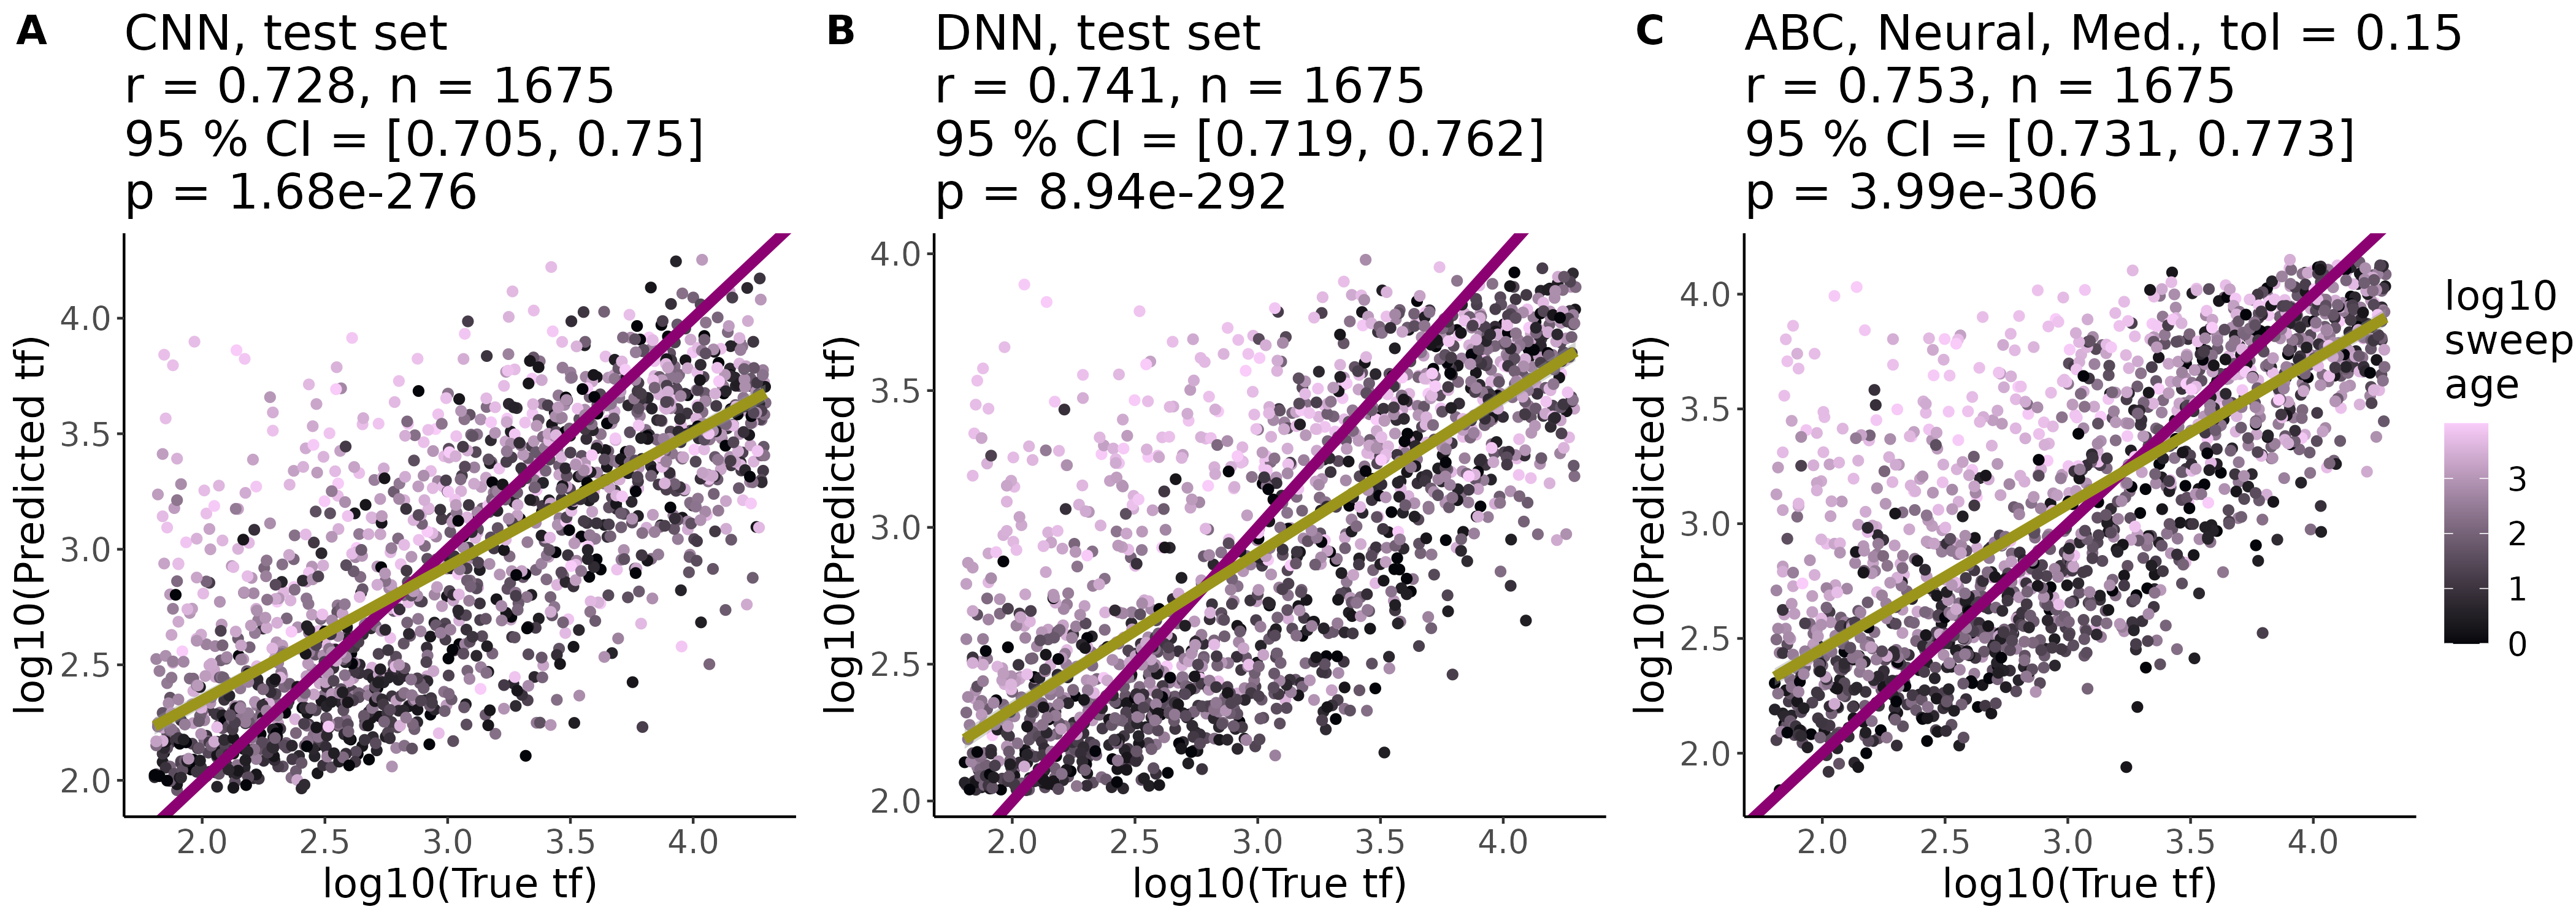
\includegraphics[width=\textwidth]{figures/chapter_4/best_models_constant_2025-03-04.png}
    \caption{\textbf{CNNs perform similarly to DNNs and ABC in a constantly sized population.} Performance of best (A) CNN, (B) DNN, and (C) ABC models at predicting $t_f$ under a constant demographic scenario. For each model, we list Pearson correlation coefficients between predicted and true values ($r$), the number of test set examples ($n$), the 95 \% confidence intervals for $r$, and the p-value for testing if $r$ is different from 0 ($p$). The purple line is the 1-1 reference line where predictions and truth are equal. The yellow line is a least squares regression line. All points are colored according to the age of the selective sweep in generations (log10 transformed).}
    \label{fig:perf_constant}
\end{figure}

\begin{figure}[H]
    \centering
    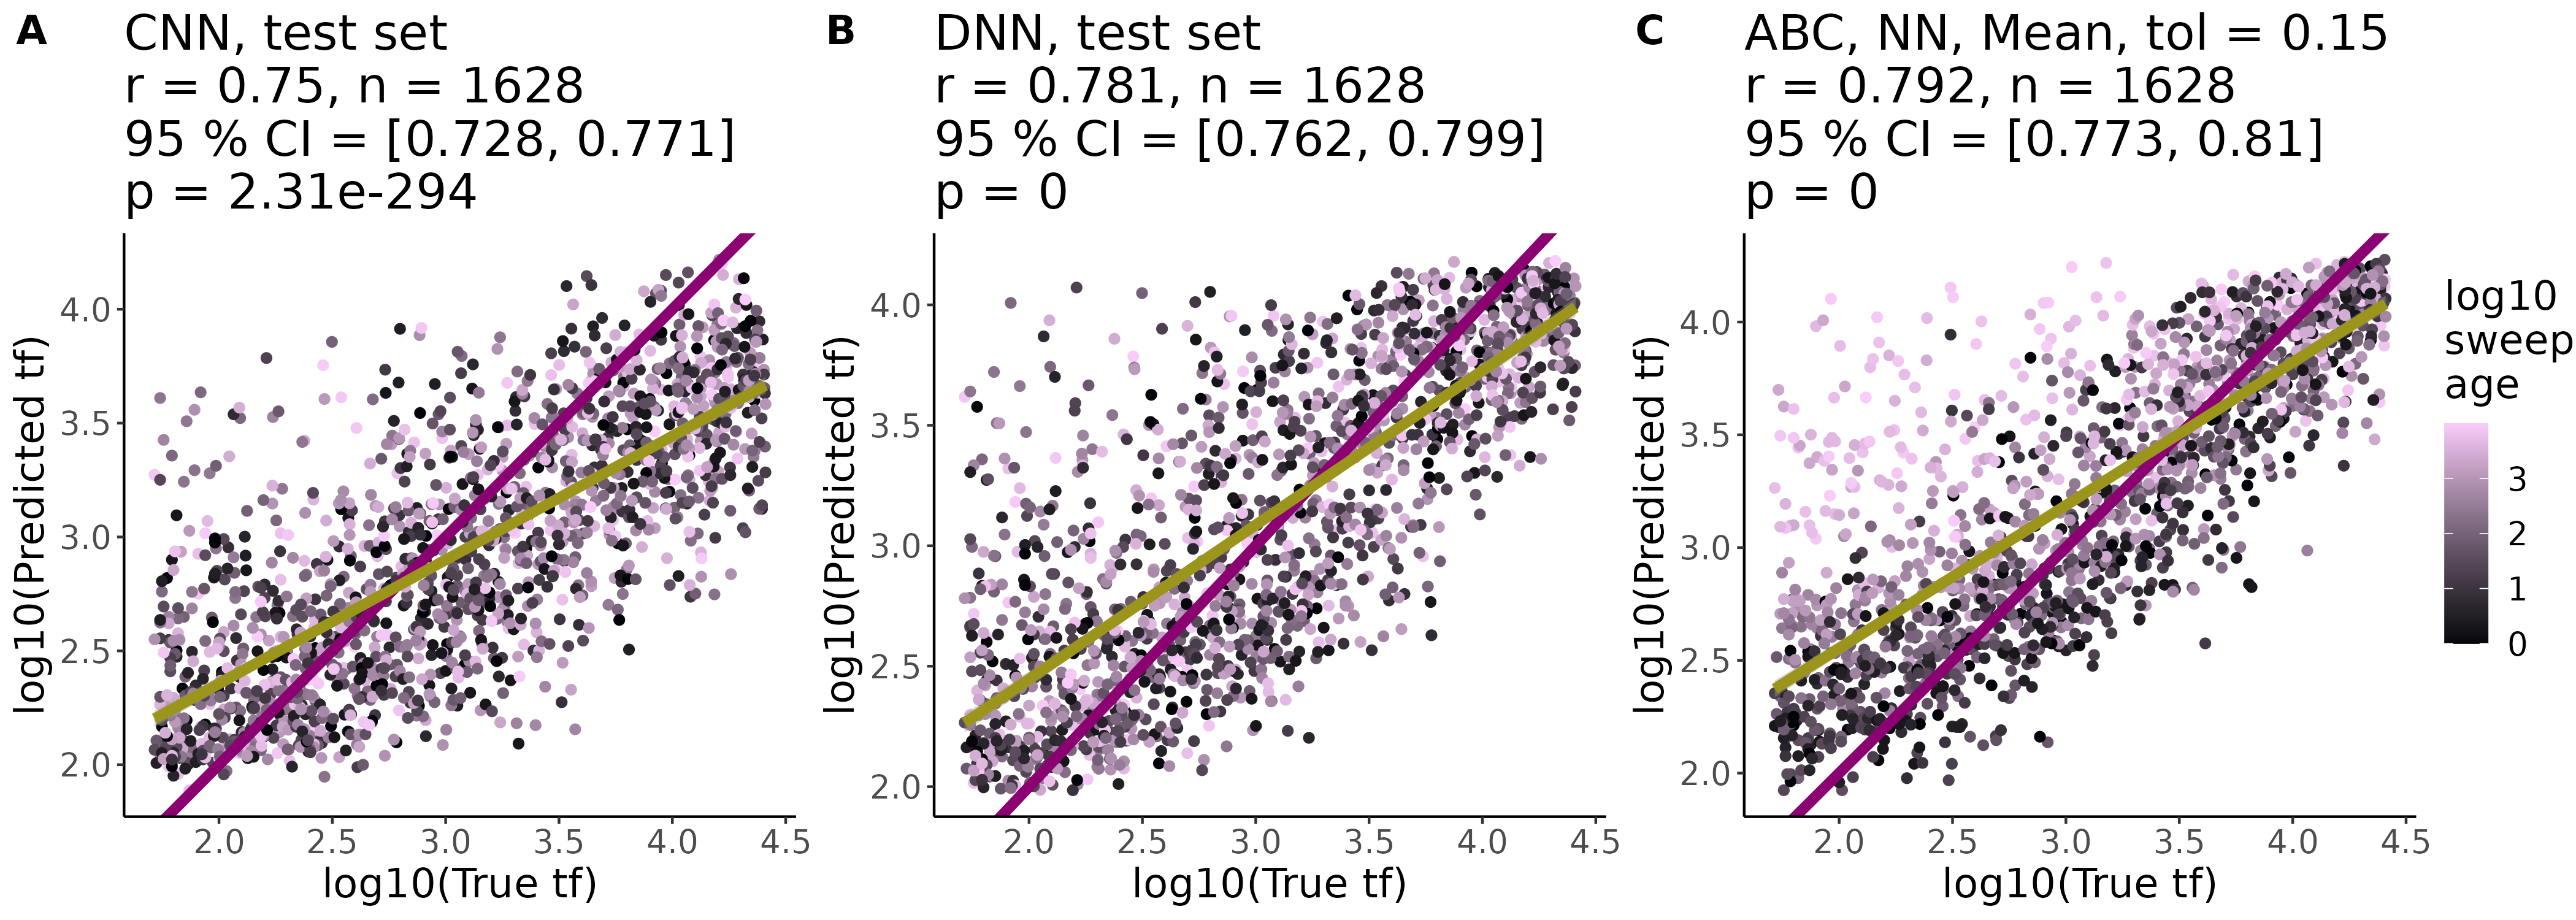
\includegraphics[width=\linewidth]{figures/chapter_4/best_models_growth_2025-03-05.png}
    \caption{\textbf{CNNs and DNNs and ABC in a growing population.} Performance of best (A) CNN, (B) DNN, and (C) ABC models at predicting $t_f$ under a constant demographic scenario. For each model, we list Pearson correlation coefficients between predicted and true values ($r$), the number of test set examples ($n$), the 95 \% confidence intervals for $r$, and the p-value for testing if $r$ is different from 0 ($p$). The purple line is the 1-1 reference line where predictions and truth are equal. The yellow line is a least squares regression line. All points are colored according to the age of the selective sweep in generations (log10 transformed).}
    \label{fig:perf_growth}
\end{figure}

\subsection*{Discussion}
%\addcontentsline{toc}{subsubsection}{4.4: Discussion}

\begin{double}

We simulated approximately 250,000 selective sweeps across a range of parameters and demographic scenarios, then used those simulations to train CNNs, DNNs, and ABC models to predict $t_f$. Our hypothesis was that CNNs could potentially better disentangle $t_f$ from $t_a$ and thus be better at predicting $t_f$. Our simulations reflected a core challenge in the problem of distinguishing $t_f$ from $t_a$: sweeps with high $t_f$ and low $t_a$ (i.e. slow, young sweeps) leave similar signatures as sweeps with low $t_f$ and high $t_a$ (i.e. fast, old sweeps, Figure \ref{fig:ident}C). Each of the 17 selective sweep statistics we calculated explained additional variation in $t_f + t_a$ (Figure \ref{fig:partrsq}). In the end, our models trained on  summary statistics (DNN and ABC) performed similarly to CNNs, which were trained on images of genotype matrices (Figure \ref{fig:perf_constant}, \ref{fig:perf_growth}, E1-E3).

Similar to previous studies on estimating coalescent times \citep{y_c_brandt_evaluation_2022}, we noticed a general bias where models overestimate low values of $t_f$ and underestimate high values of $t_f$ (Figure \ref{fig:perf_constant}, \ref{fig:perf_growth}, E1-E3). This is mostly likely due to a general identifiability problem where old, fast sweeps leave similar signatures as young, slow sweeps (Figure \ref{fig:ident}, E4-E7). However, in the growth demography scenario CNNs and DNNs were apparently better able to disentangle $t_f$ and $t_a$ (Figure \ref{fig:perf_growth}A and \ref{fig:perf_growth}B) compared to ABC (Figure \ref{fig:perf_growth} C). This is possibly because two important signatures of sweeps, an excess of common alleles in site frequency spectra and excessive linkage, persist for longer in populations with higher $N_e$ \citep{przeworski_signature_2002}. Thus, the signatures of a short $t_f$ persist for longer and prevent (or at least delay) confusion of old, fast sweeps with slow, young sweeps. The second case where ABC and CNNs diverged was the cyclic demography scenario, where the correlation between true and predicted $t_f$ was lower for the CNN than the DNN and ABC, even though the DNN and ABC maintained a similar correlation compared to the constant demography scenario (Figure \ref{fig:cycle_comparison}). This is potentially because repeated population bottlenecks have several consequences for the dynamics of sweeps \citep{wilson_soft_2014}. In our case, if population bottlenecks are softening the sweeps, then it's possible that the CNN has trouble making predictions for this type of sweep compared to DNNs and ABC which are fed statistics specifically tuned for soft sweeps (H2H1, H123, etc.).

Summary statistics were overall effective at predicting $t_f$ from unphased genotype data (Figure \ref{fig:perf_constant}B-C, \ref{fig:perf_growth}B-C). Our hypothesis was that CNNs could potentially identify new signatures besides known summary statistics and thus better predict $t_f$ \citep{hahn_estimating_2025}. However, the fact that ABC based on summary statistics performs the same or slightly better than a CNN suggests unphased genotype matrices do not contain signals for $t_f$ that are not already captured by summary statistics. Many CNNs that classify selective sweeps use summary statistics partly to ease interpretability \citep{kern_diploshic_2018, lauterbur_versatile_2023}, but previous studies have also show CNNs trained on genotype matrices largely learn to reproduce summary statistics \citep{cecil_convolutional_2023}. It is still possible though that additional signatures of $t_f$ not already described by summary statistics do arise in other demographies not explored in this study.

Two general directions forward for improving $t_f$ predictions are to tweak the prediction algorithms or include additional sources of data. Inclusion of time series data \citep{whitehouse_timesweeper_2023} or phasing information could conceivably aid $t_f$ prediction, but these are limited to cases where the researchers have ancient samples or an understanding of a recombination landscape. Another option would be to include data from more than one population \citep{yair_timing_2021}. Population differentiation provides information on the split time between populations and if a sweep is shared across populations, that would suggest that the sweep happened before the population split \citep{yair_timing_2021}. The difficulty here is that one needs to know or derive a model of the population split and admixture beforehand so that it can be properly simulated. A combination of both including additional data types and tuning models will most likely be the fruitful path forward.

\end{double}

\vspace{12pt}

\subsection*{Data availability}

\begin{double}
Supplemental figures are in Appendix E. Our entire analysis is available as a snakemake workflow, packaged here: \url{https://github.com/milesroberts-123/selection-demography-cnn}.
\end{double}

\newpage

\addcontentsline{toc}{subsection}{BIBLIOGRAPHY}
\bibliography{references,olivia_refs}

\newpage


\section*{APPENDIX A: SUPPLEMENTAL FIGURES FOR CHAPTER 1}
\addcontentsline{toc}{subsection}{APPENDIX A: SUPPLEMENTAL FIGURES FOR CHAPTER 1}

\setcounter{figure}{0}
\renewcommand{\figurename}{Figure}
\renewcommand{\thefigure}{A\arabic{figure}}

\vspace{12pt}

\subsection*{General data curation}

\begin{figure}[H]
\centering
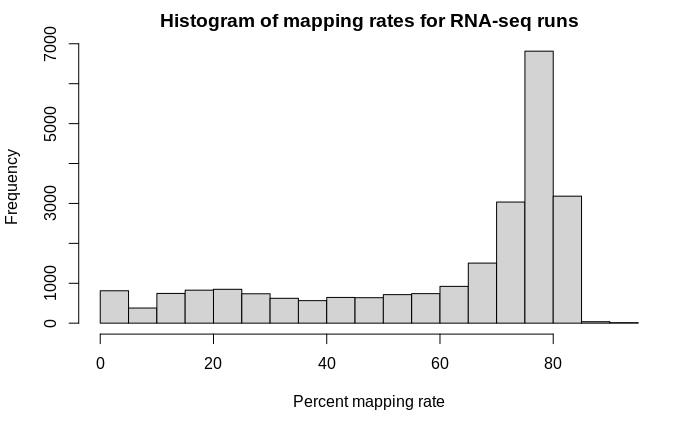
\includegraphics[width = \linewidth]{figures/appendix_a/histogram_mappingRates_2022-07-18.jpeg}
\caption{\textbf{Histogram of mapping rates for RNA-seq runs.} Bin width is 5 \%.}%
\end{figure}

\newpage

\begin{figure}[H]
\centering
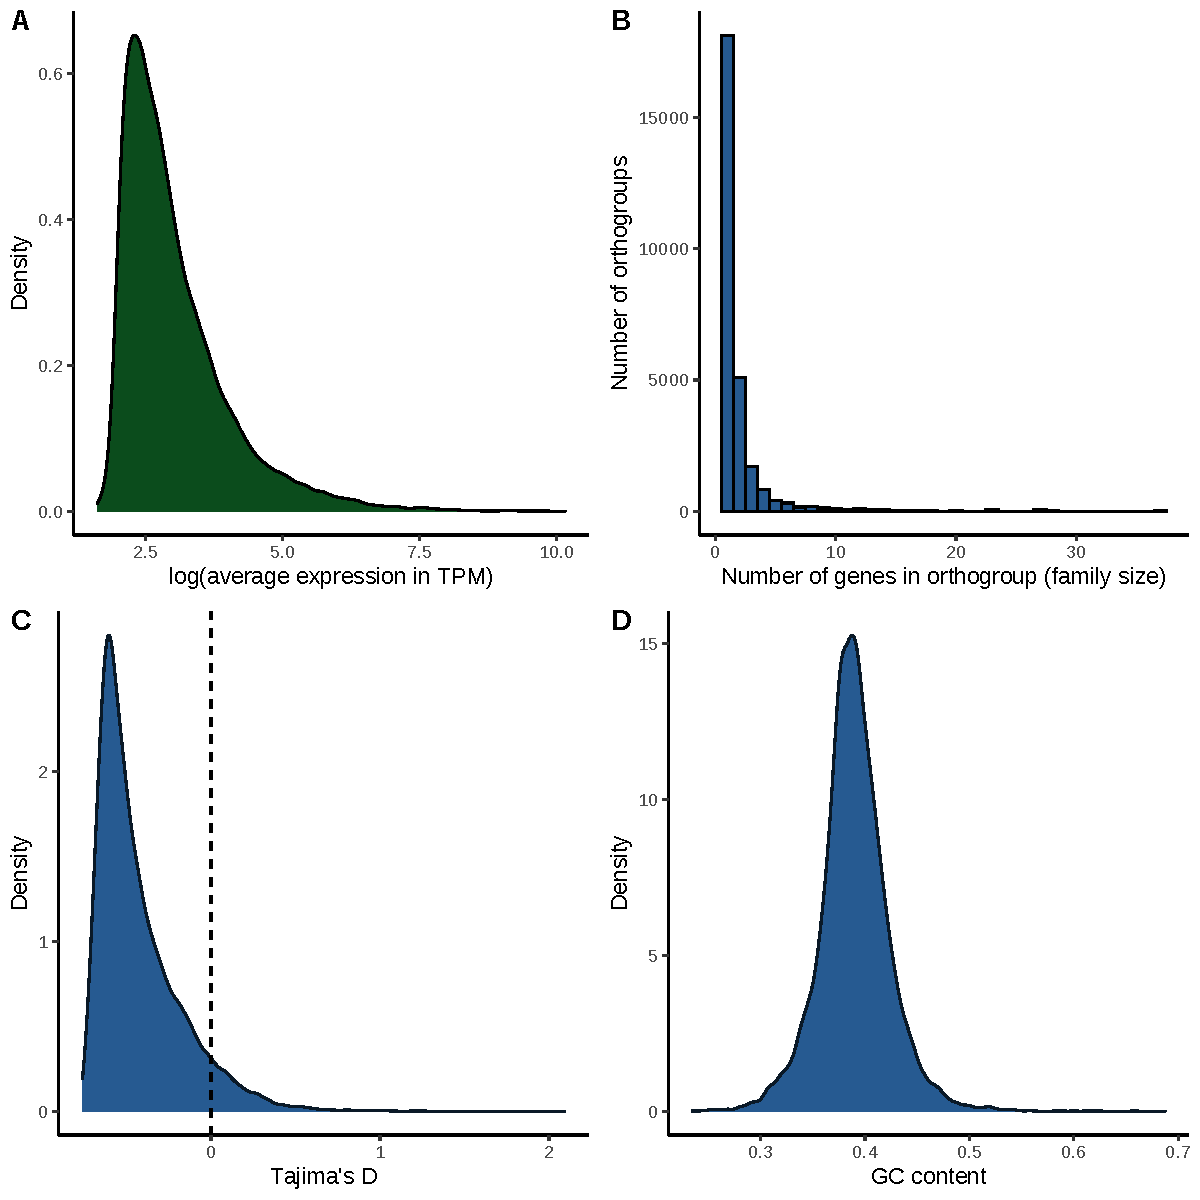
\includegraphics[width = \linewidth]{figures/appendix_a/histogramsOfMoreKeyVariables.pdf}
\caption{\textbf{Histograms of other key variables for the genes included in this study.}}%
\end{figure}

\newpage

\begin{figure}[H]
\centering
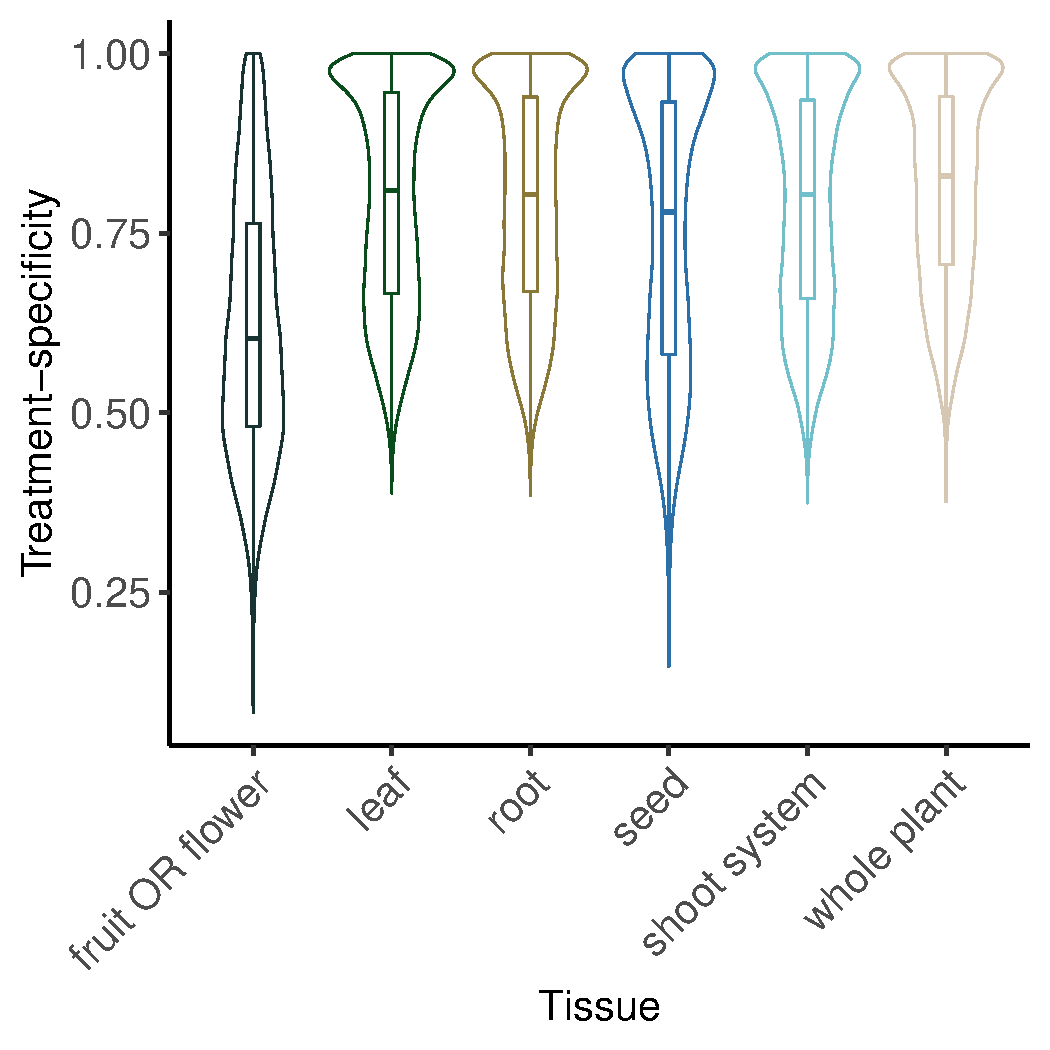
\includegraphics[width = \linewidth]{figures/appendix_a/densityPlotsOfTreatmentSpecificity.pdf}
\caption{\textbf{Violin plot of treatment-specificity in gene expression for six tissue categories.}}%
\end{figure}

\newpage

\begin{figure}[H]
\centering
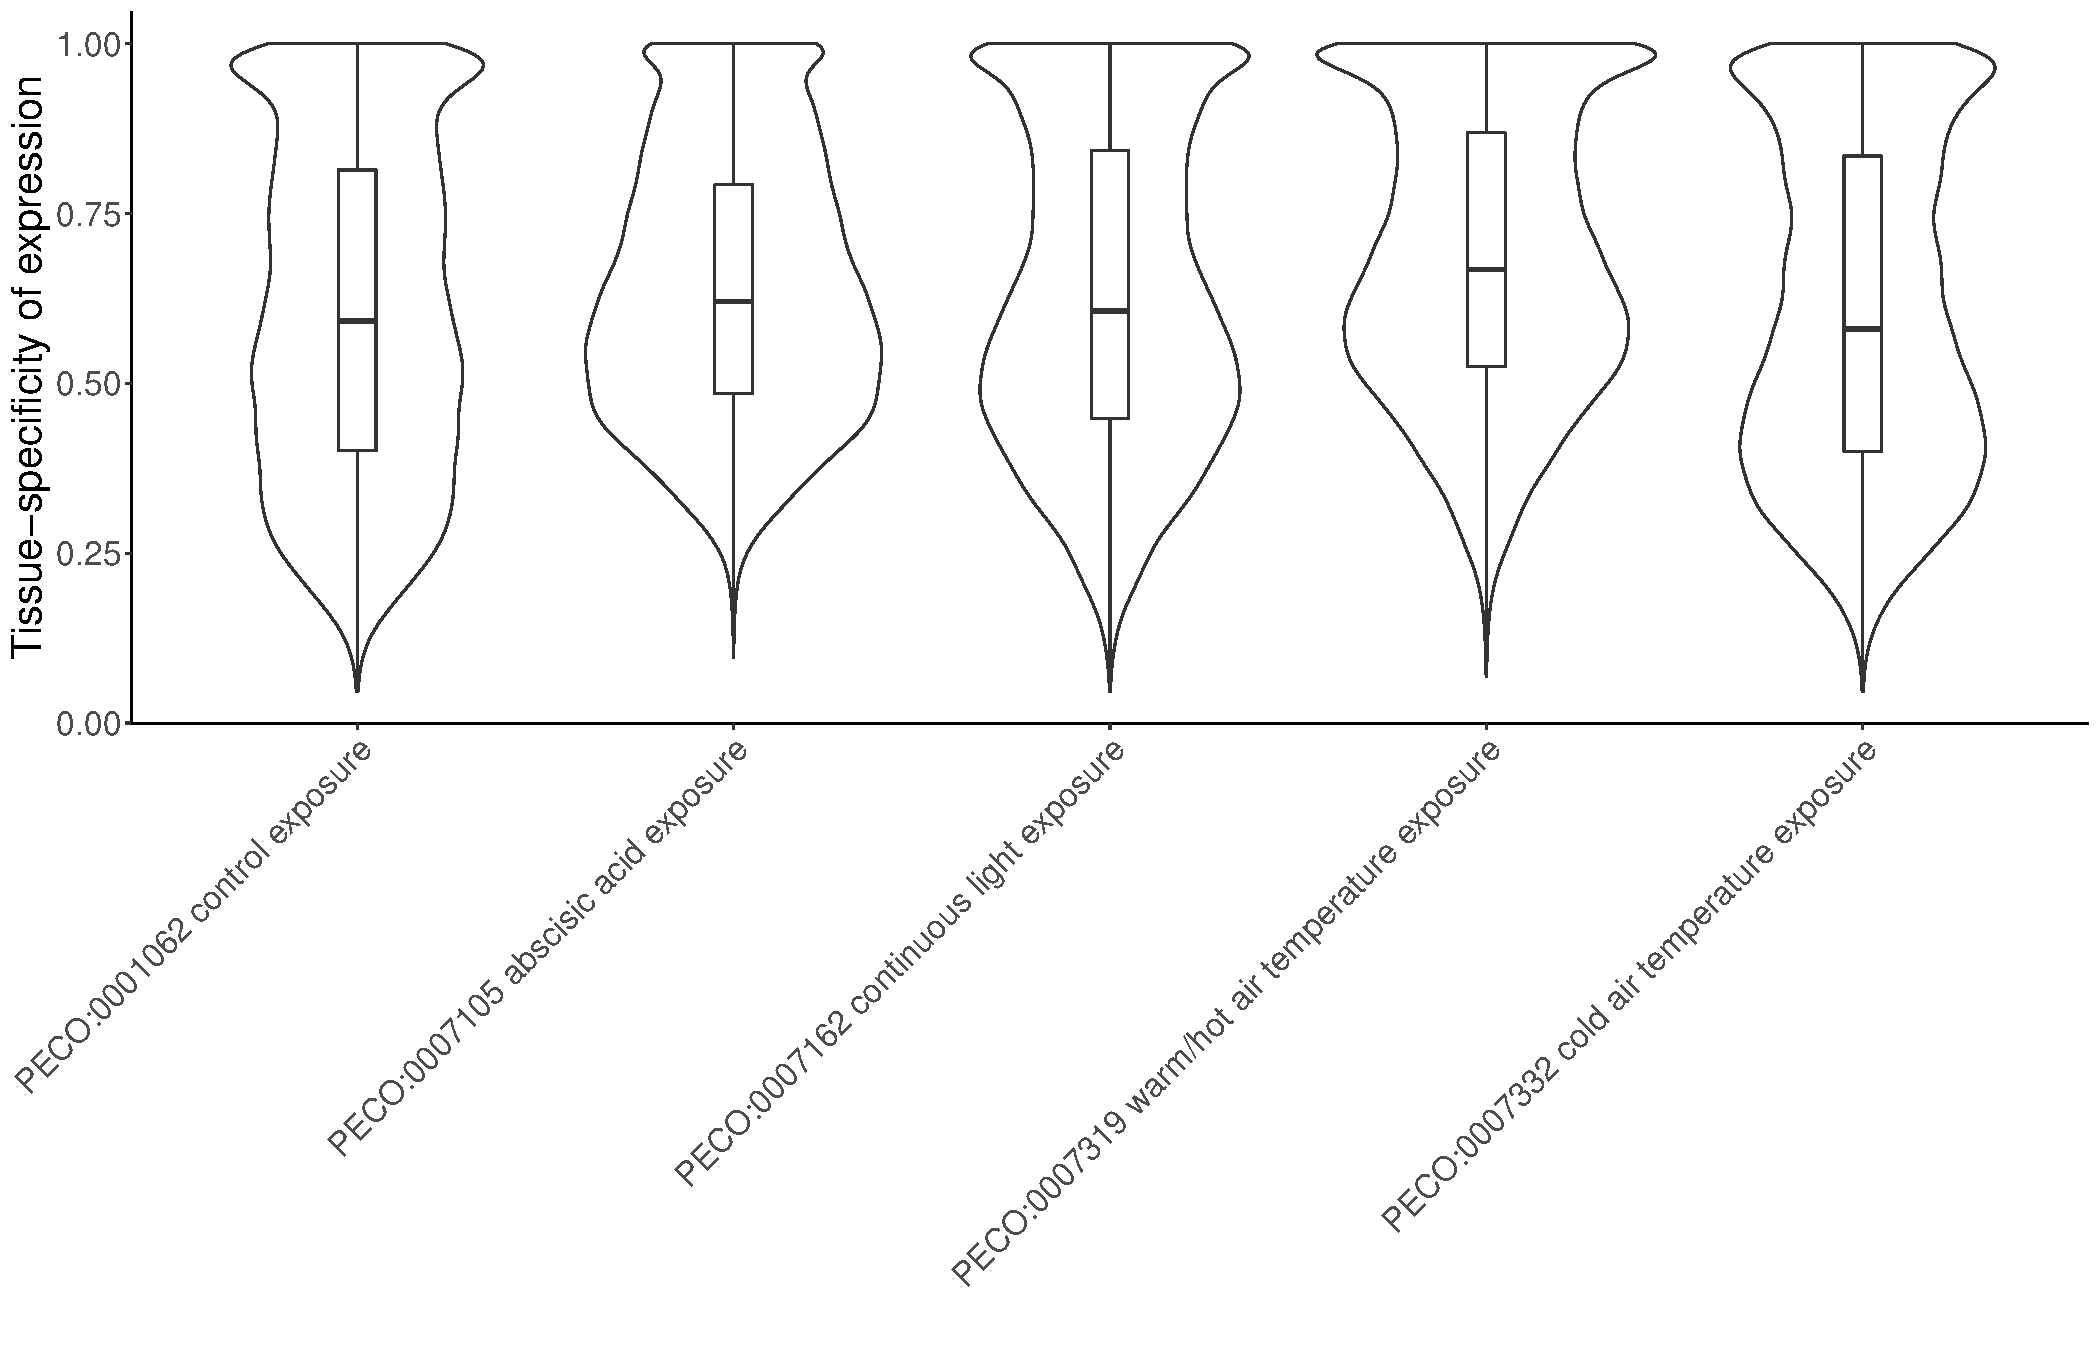
\includegraphics[width = \linewidth]{figures/appendix_a/densityPlotsOfTissueSpecificity.pdf}
\caption{\textbf{Violin plot of tissue-specificity in gene expression by treatment type.} Only the five treatments shown had samples from all six tissue types.}%
\end{figure}

\newpage

\begin{figure}[H]
\centering
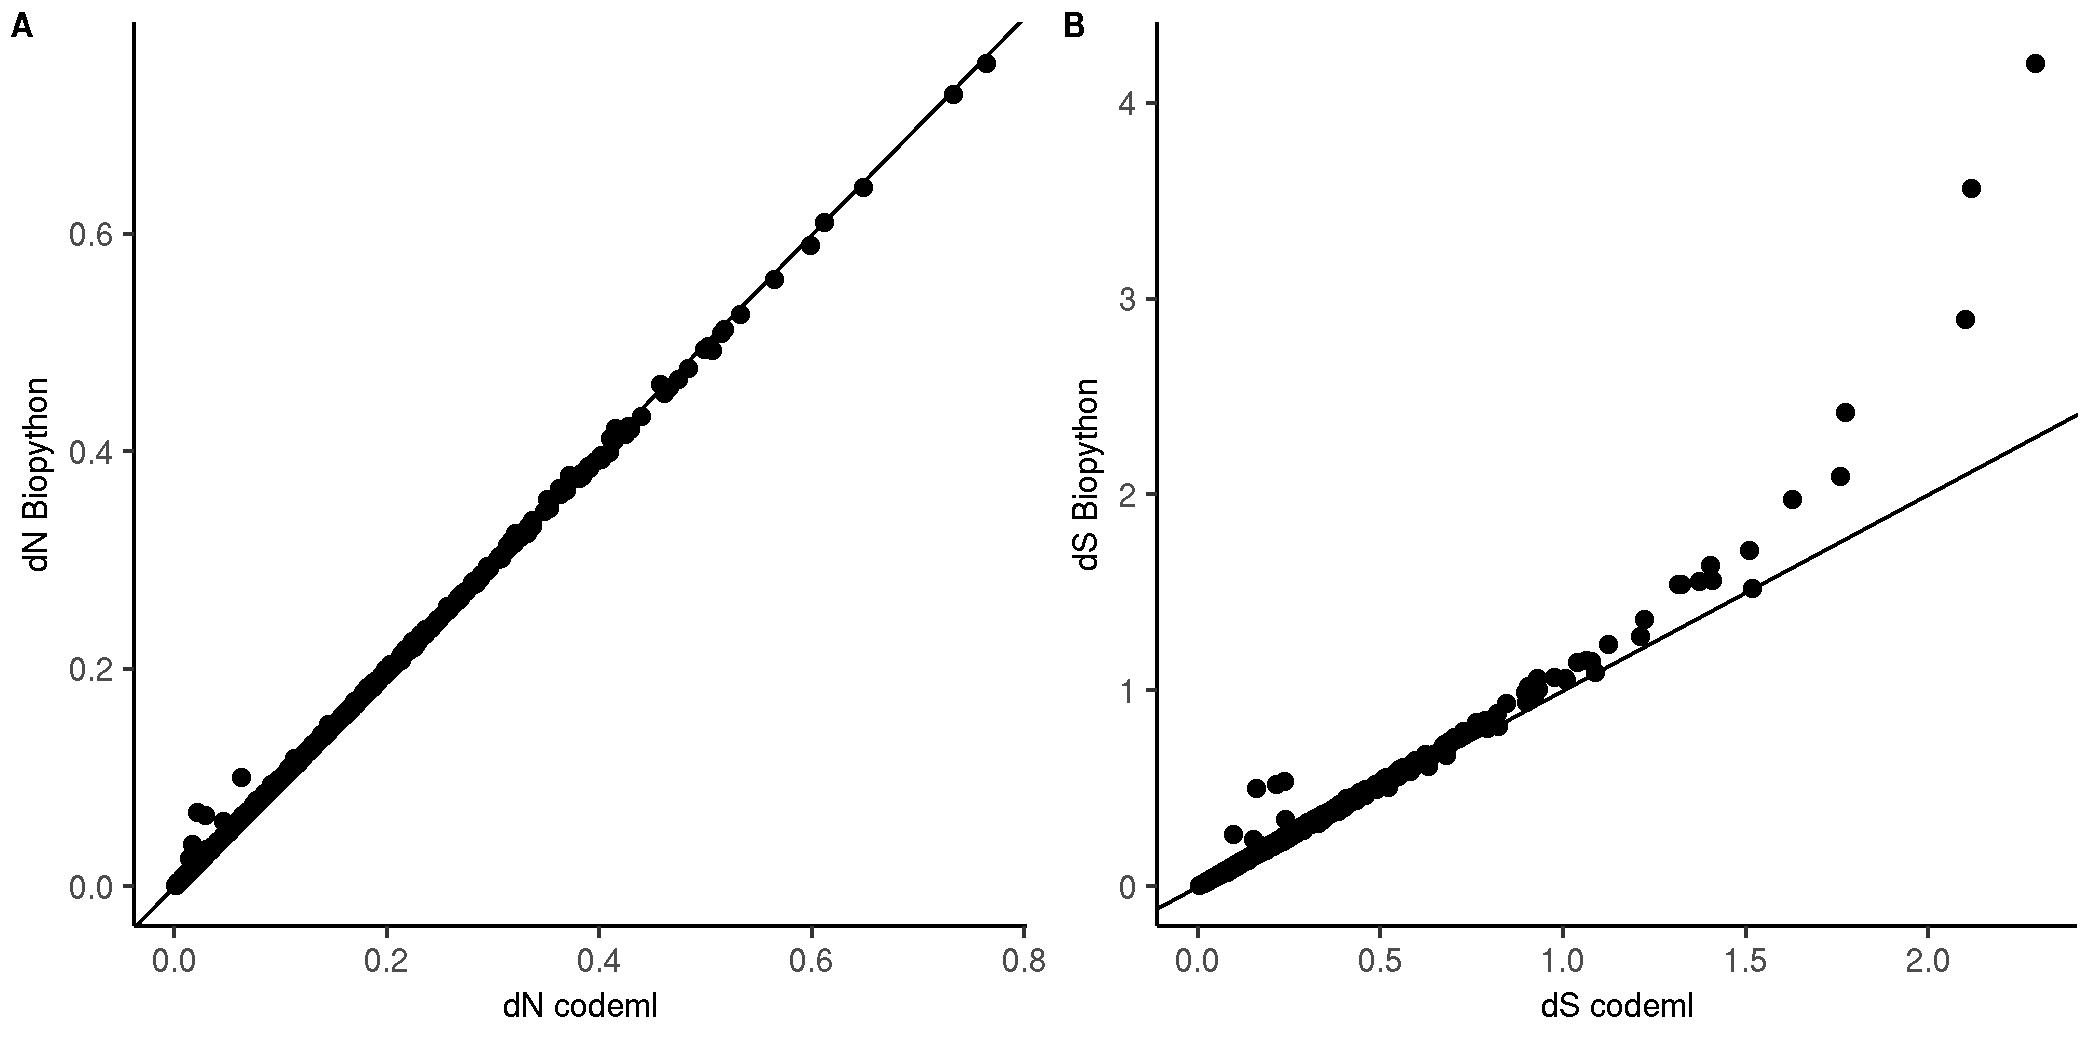
\includegraphics[width = \linewidth]{figures/appendix_a/codemlVsBiopythonComparison_2022-08-11.jpeg}
\caption{\textbf{Comparing $dN$ and $dS$ values returned from codeml and the custom biopython script used in this study.} Line shows exact match between codeml and biopython methods. Genes with saturating divergence ($dS > 1$) were excluded from partial correlation analyses.}%
\end{figure}

\subsection*{Partial correlations on overall dataset}

\begin{figure}[H]
\centering
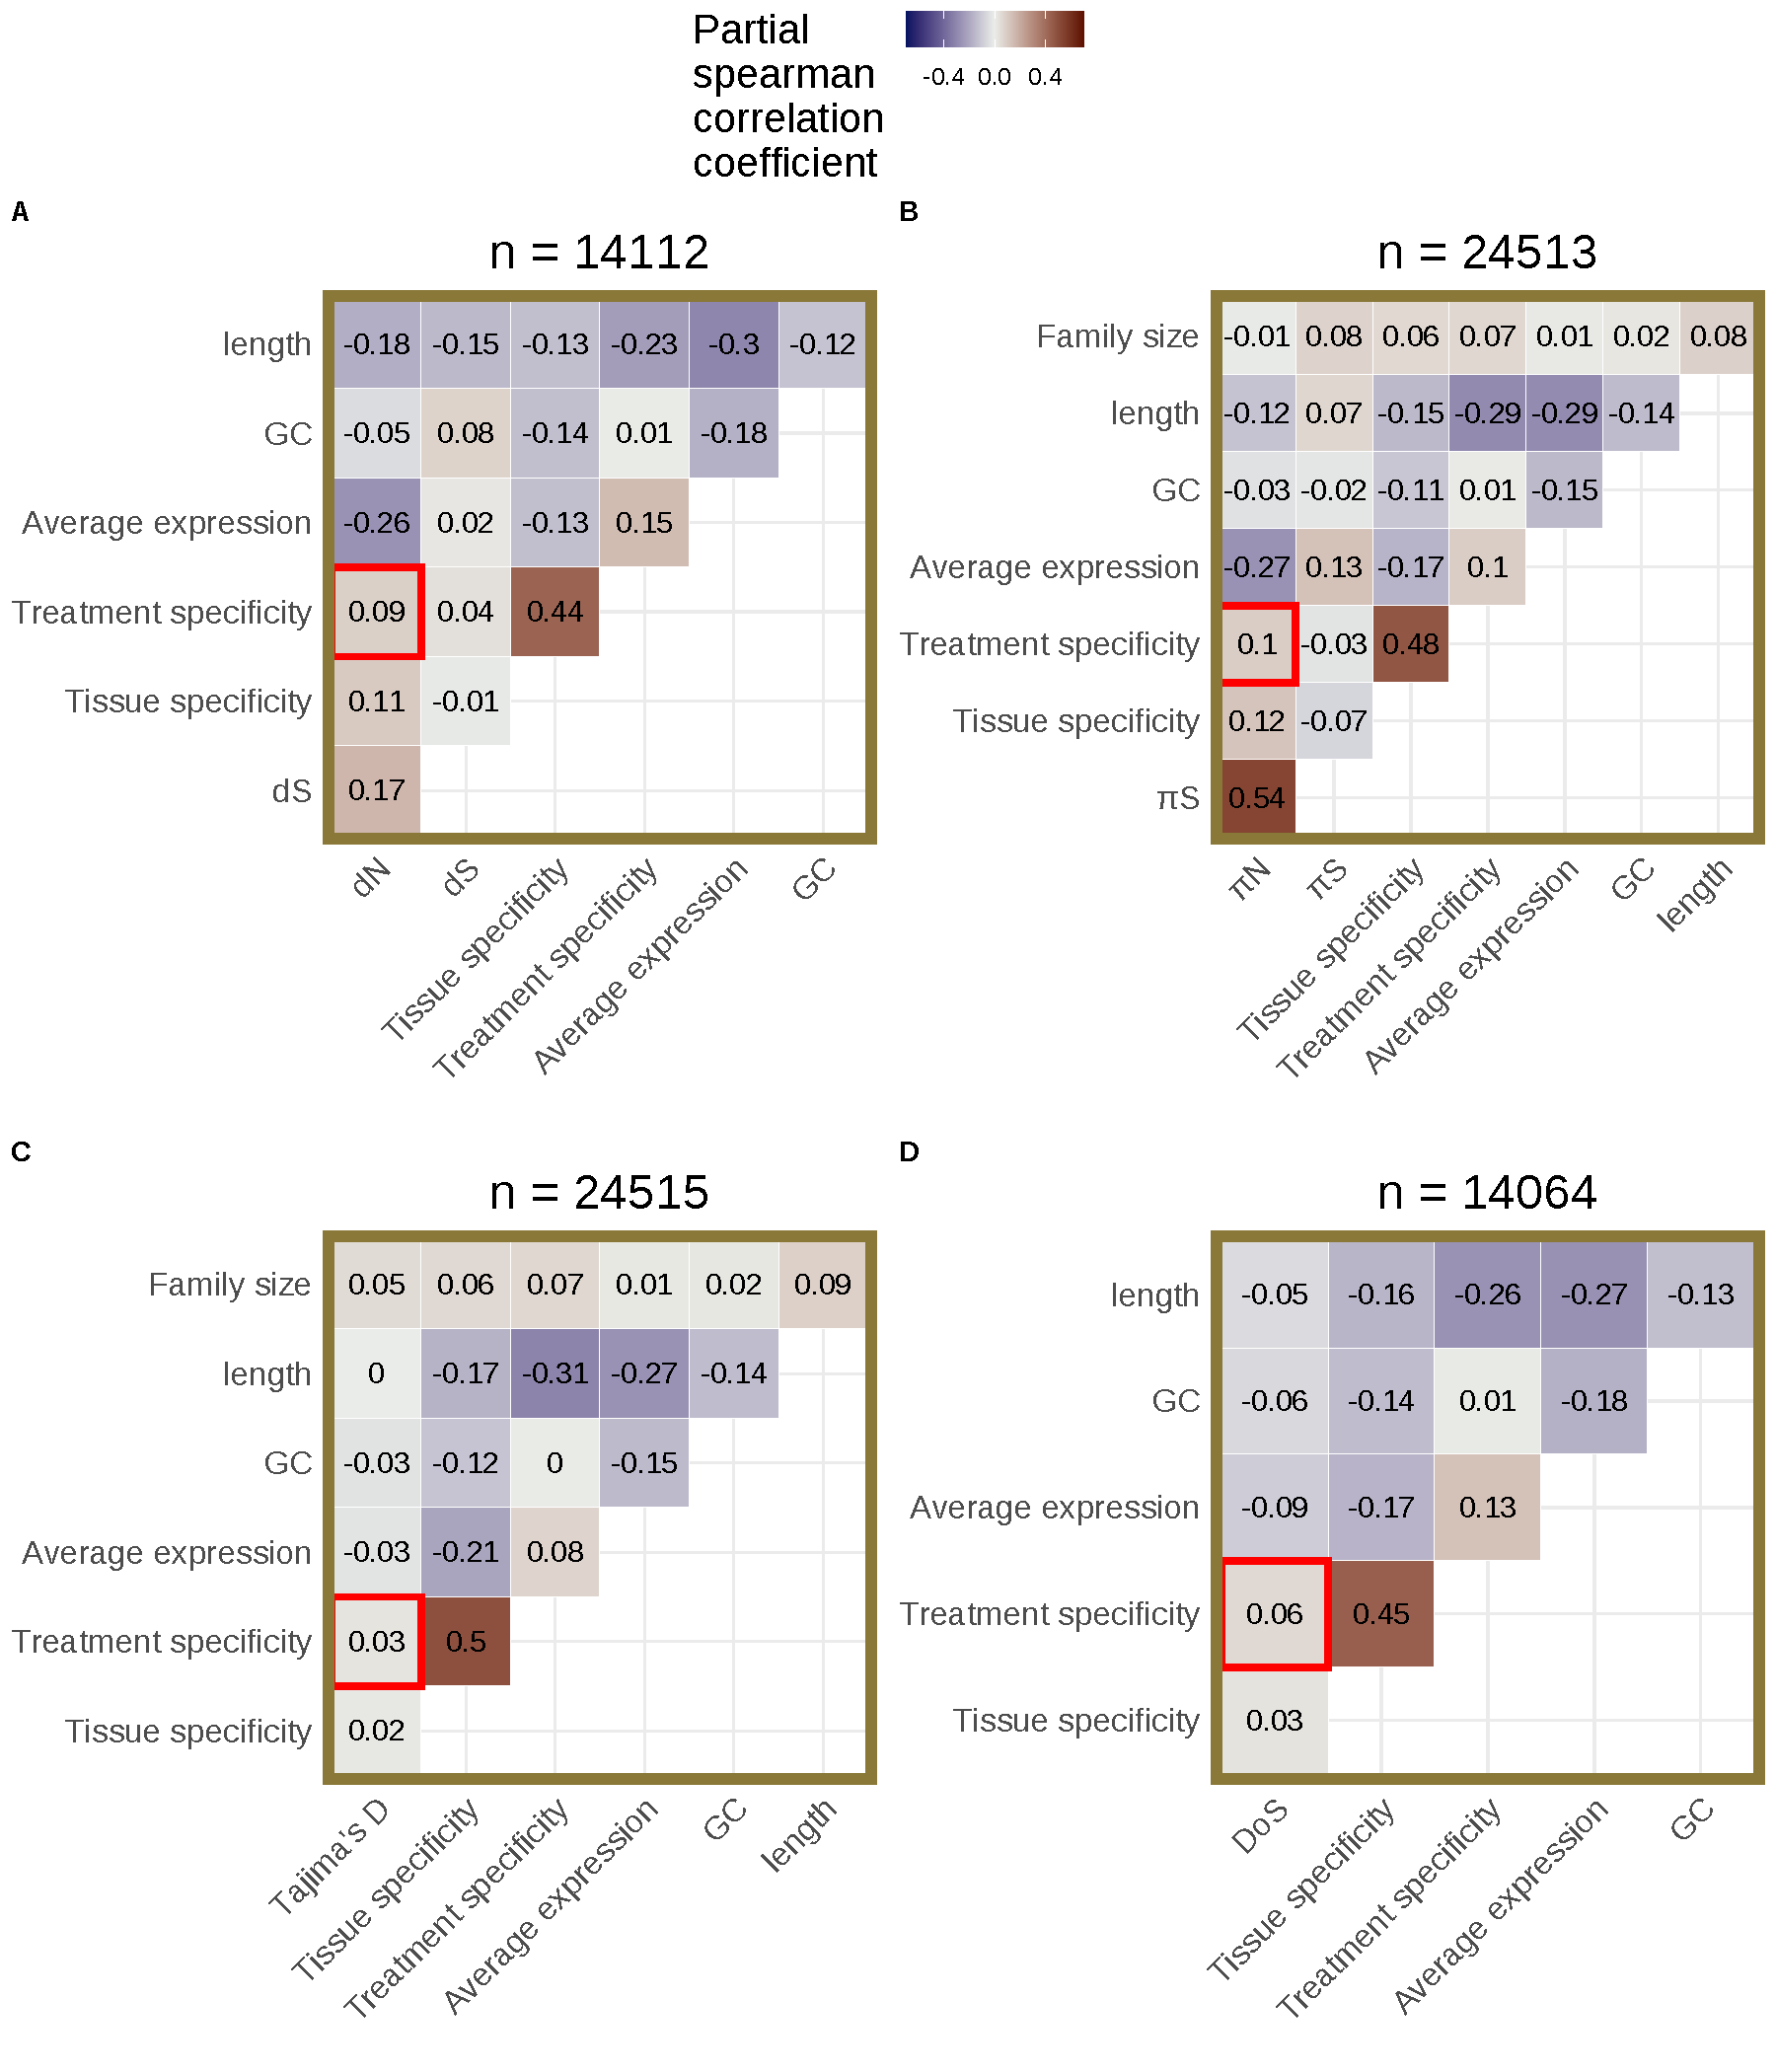
\includegraphics[width = 0.95\linewidth]{figures/appendix_a/partialCorrelations_withTissueSpecificity_root_2023-02-20.pdf}
\caption{\textbf{Partial correlation analysis for root tissue.} Partial correlations for (\textbf{A}) $dN$, (\textbf{B}) $\pi_N$, (\textbf{C}) Tajima's D, and (\textbf{D}) direction of selection (DoS) based on root data. Average expression excludes values $<$ 5 TPM and was calculated using only root tissue samples. Tissue-specificity was calculated using only control runs across all tissue categories. Treatment-specificity was calculated using only root tissue runs. The number of genes included in each partial correlation analysis (n) is listed at the top of each heatmap.}%
\end{figure}

\newpage

\begin{figure}[H]
\centering
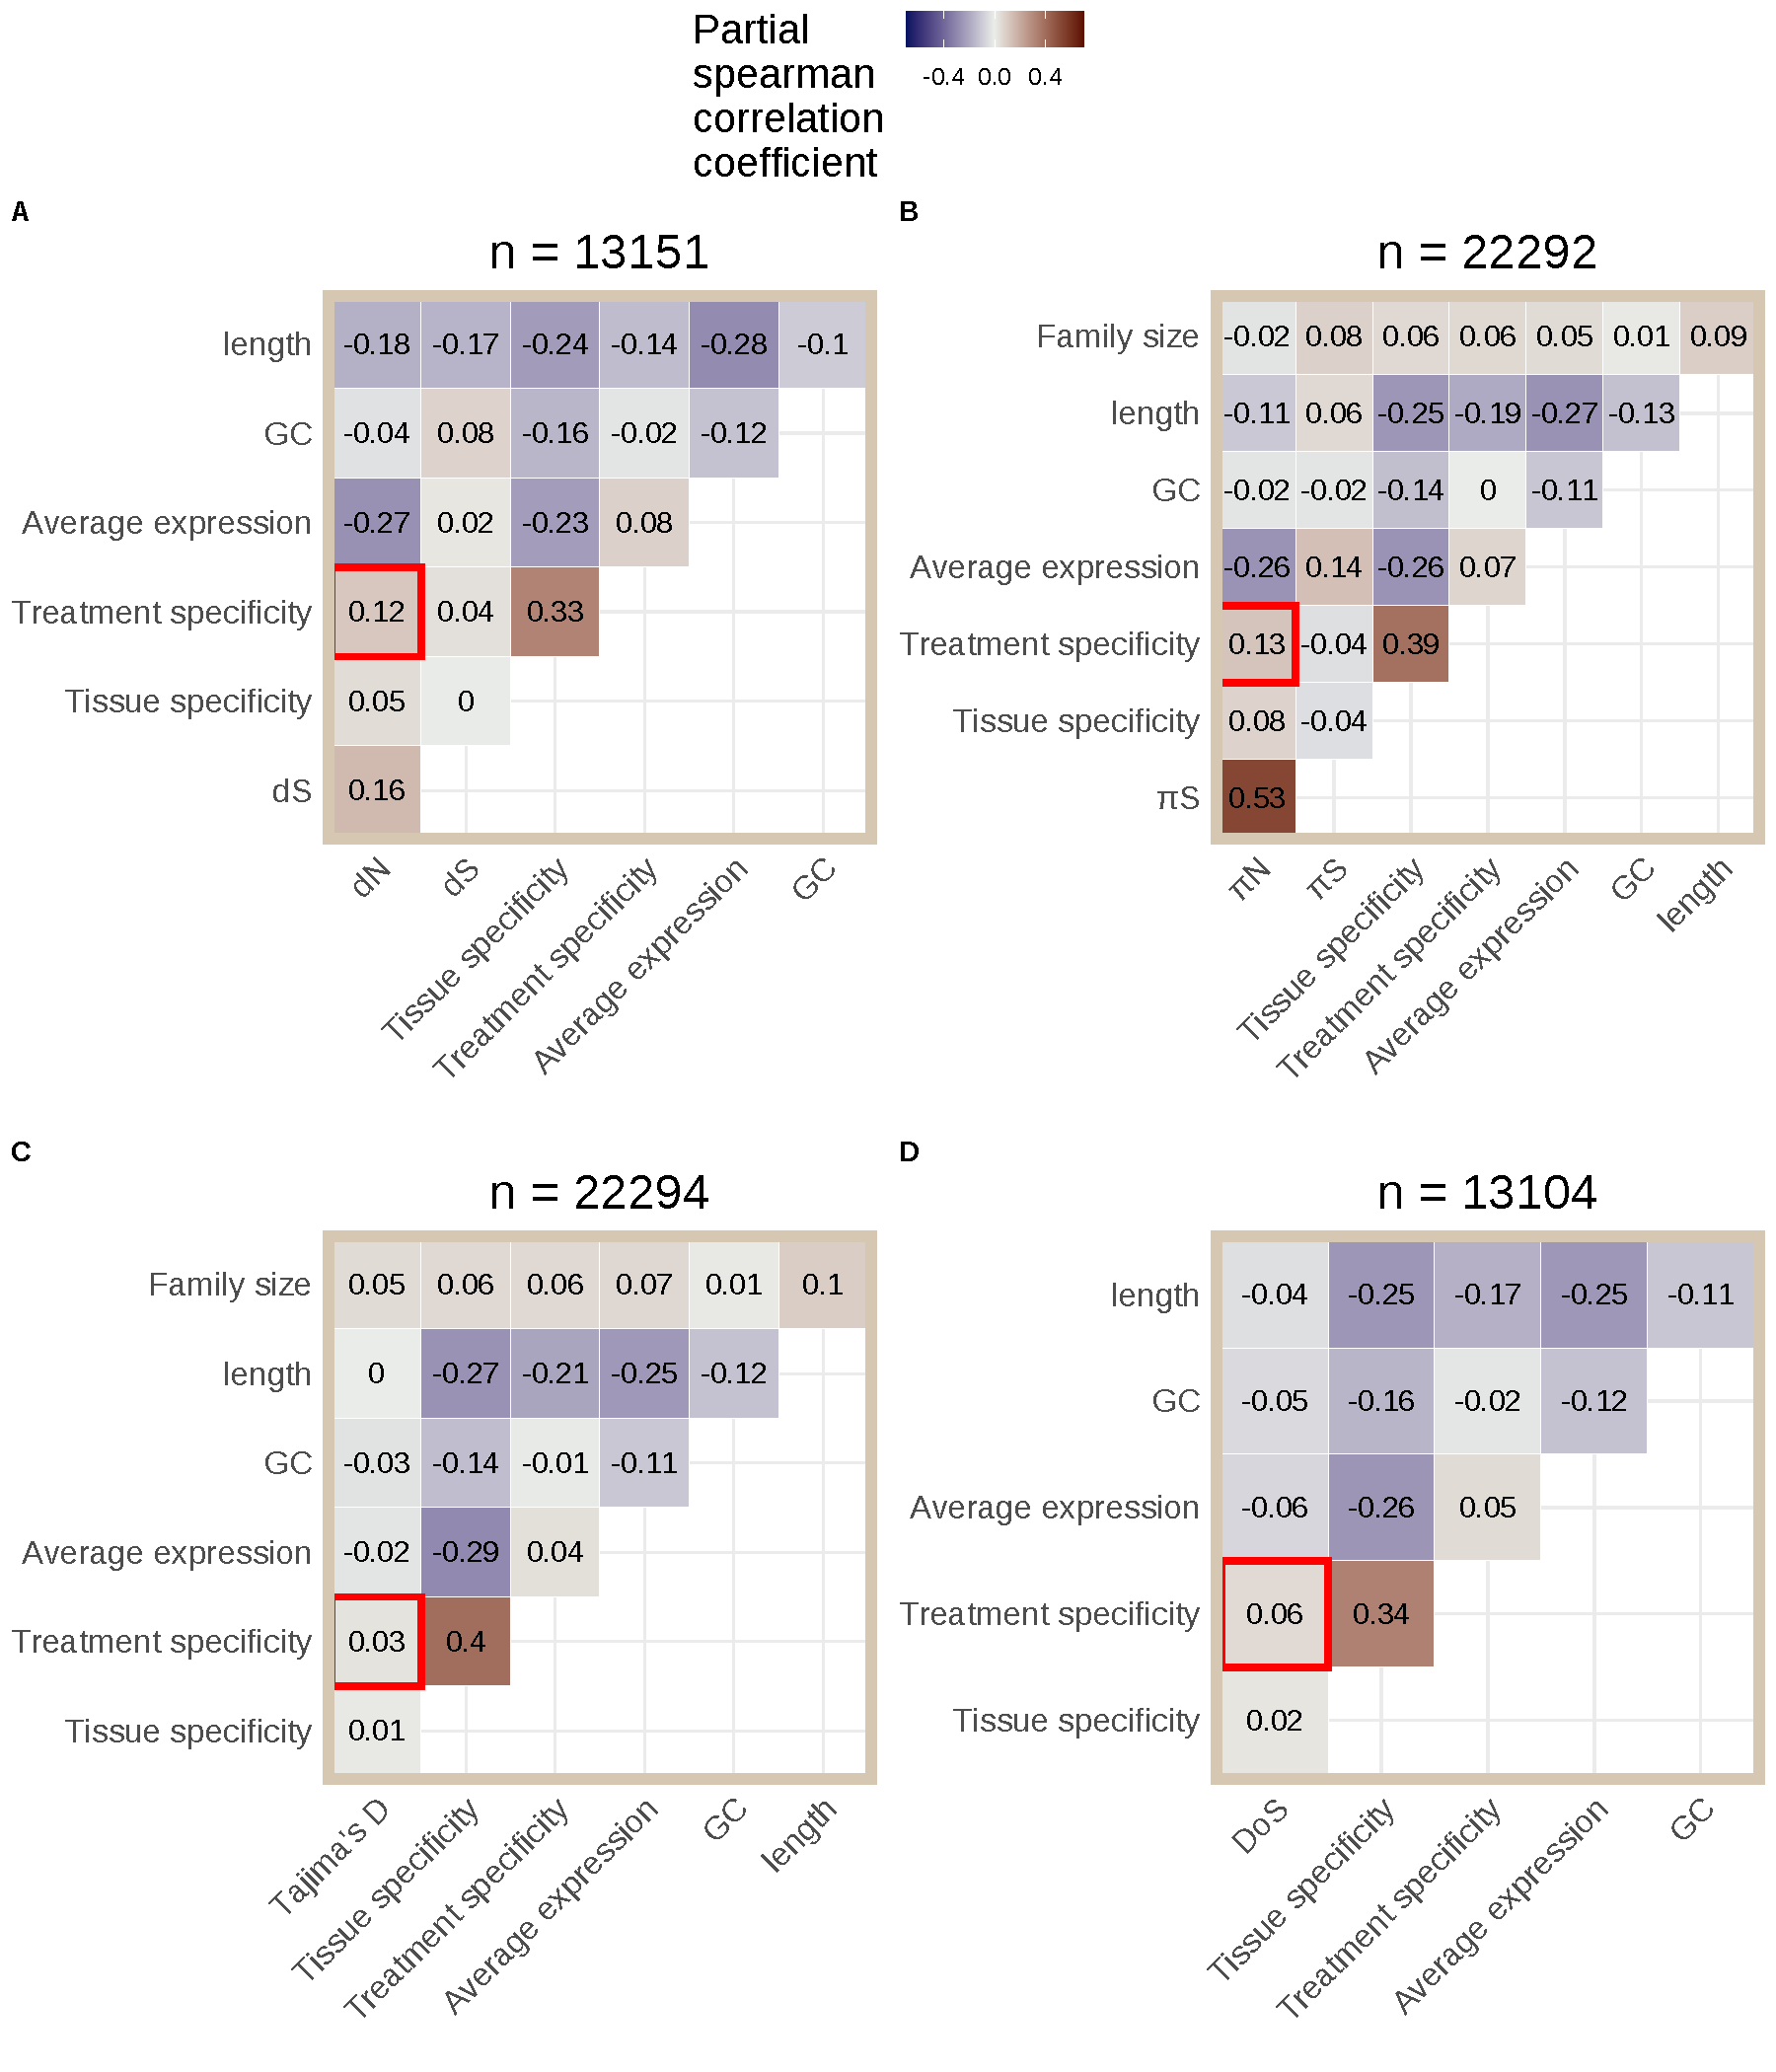
\includegraphics[width = \linewidth]{figures/appendix_a/partialCorrelations_withTissueSpecificity_wholePlant_2023-02-20.pdf}
\caption{\textbf{Partial correlation analysis for whole plant tissue.} Partial correlations for (\textbf{A}) $dN$, (\textbf{B}) $\pi_N$, (\textbf{C}) Tajima's D, and (\textbf{D}) direction of selection (DoS) based on whole plant data. Average expression excludes values $<$ 5 TPM and was calculated using only whole plant tissue samples. Tissue-specificity was calculated using only control runs across all tissue categories. Treatment-specificity was calculated using only whole plant tissue runs. The number of genes included in each partial correlation analysis (n) is listed at the top of each heatmap.}%
\end{figure}

\newpage

\begin{figure}[H]
\centering
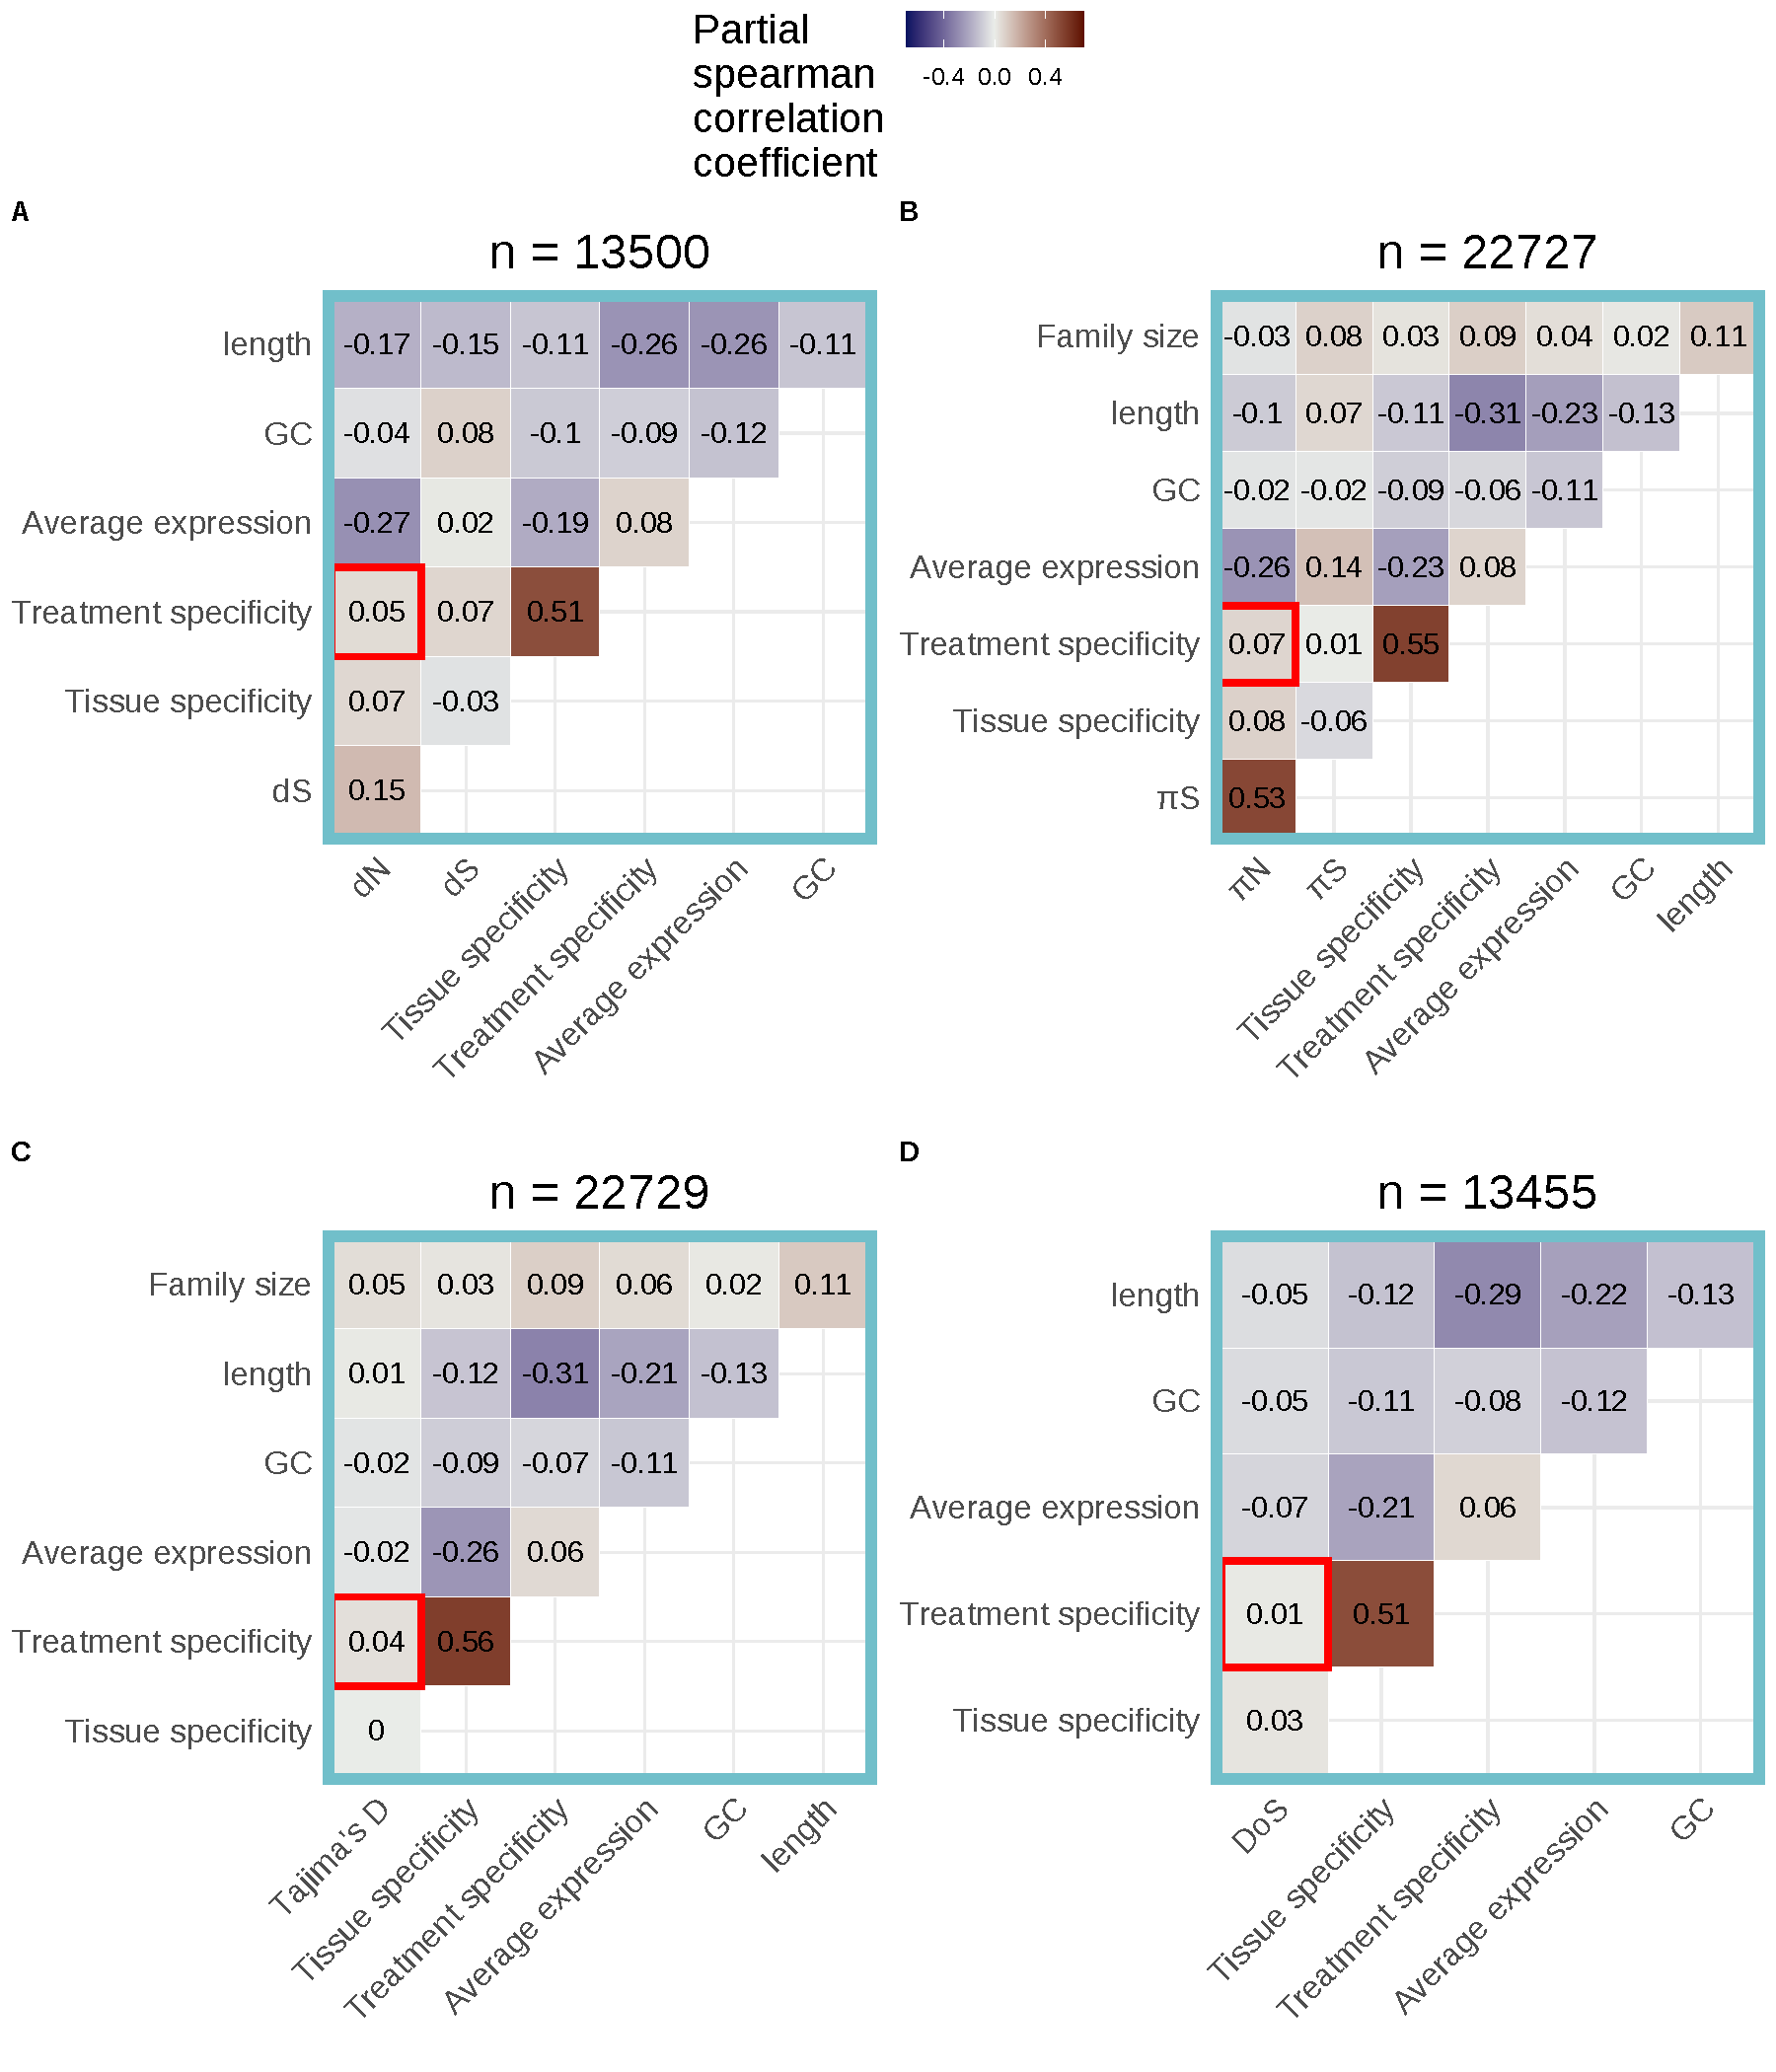
\includegraphics[width = \linewidth]{figures/appendix_a/partialCorrelations_withTissueSpecificity_shoot_2023-02-20.pdf}
\caption{\textbf{Partial correlation analysis for shoot tissue.} Partial correlations for (\textbf{A}) $dN$, (\textbf{B}) $\pi_N$, (\textbf{C}) Tajima's D, and (\textbf{D}) direction of selection (DoS) based on shoot data. Average expression excludes values $<$ 5 TPM and was calculated using only shoot tissue samples. Tissue-specificity was calculated using only control runs across all tissue categories. Treatment-specificity was calculated using only shoot tissue runs. The number of genes included in each partial correlation analysis (n) is listed at the top of each heatmap.}%
\end{figure}

\newpage

\begin{figure}[H]
\centering
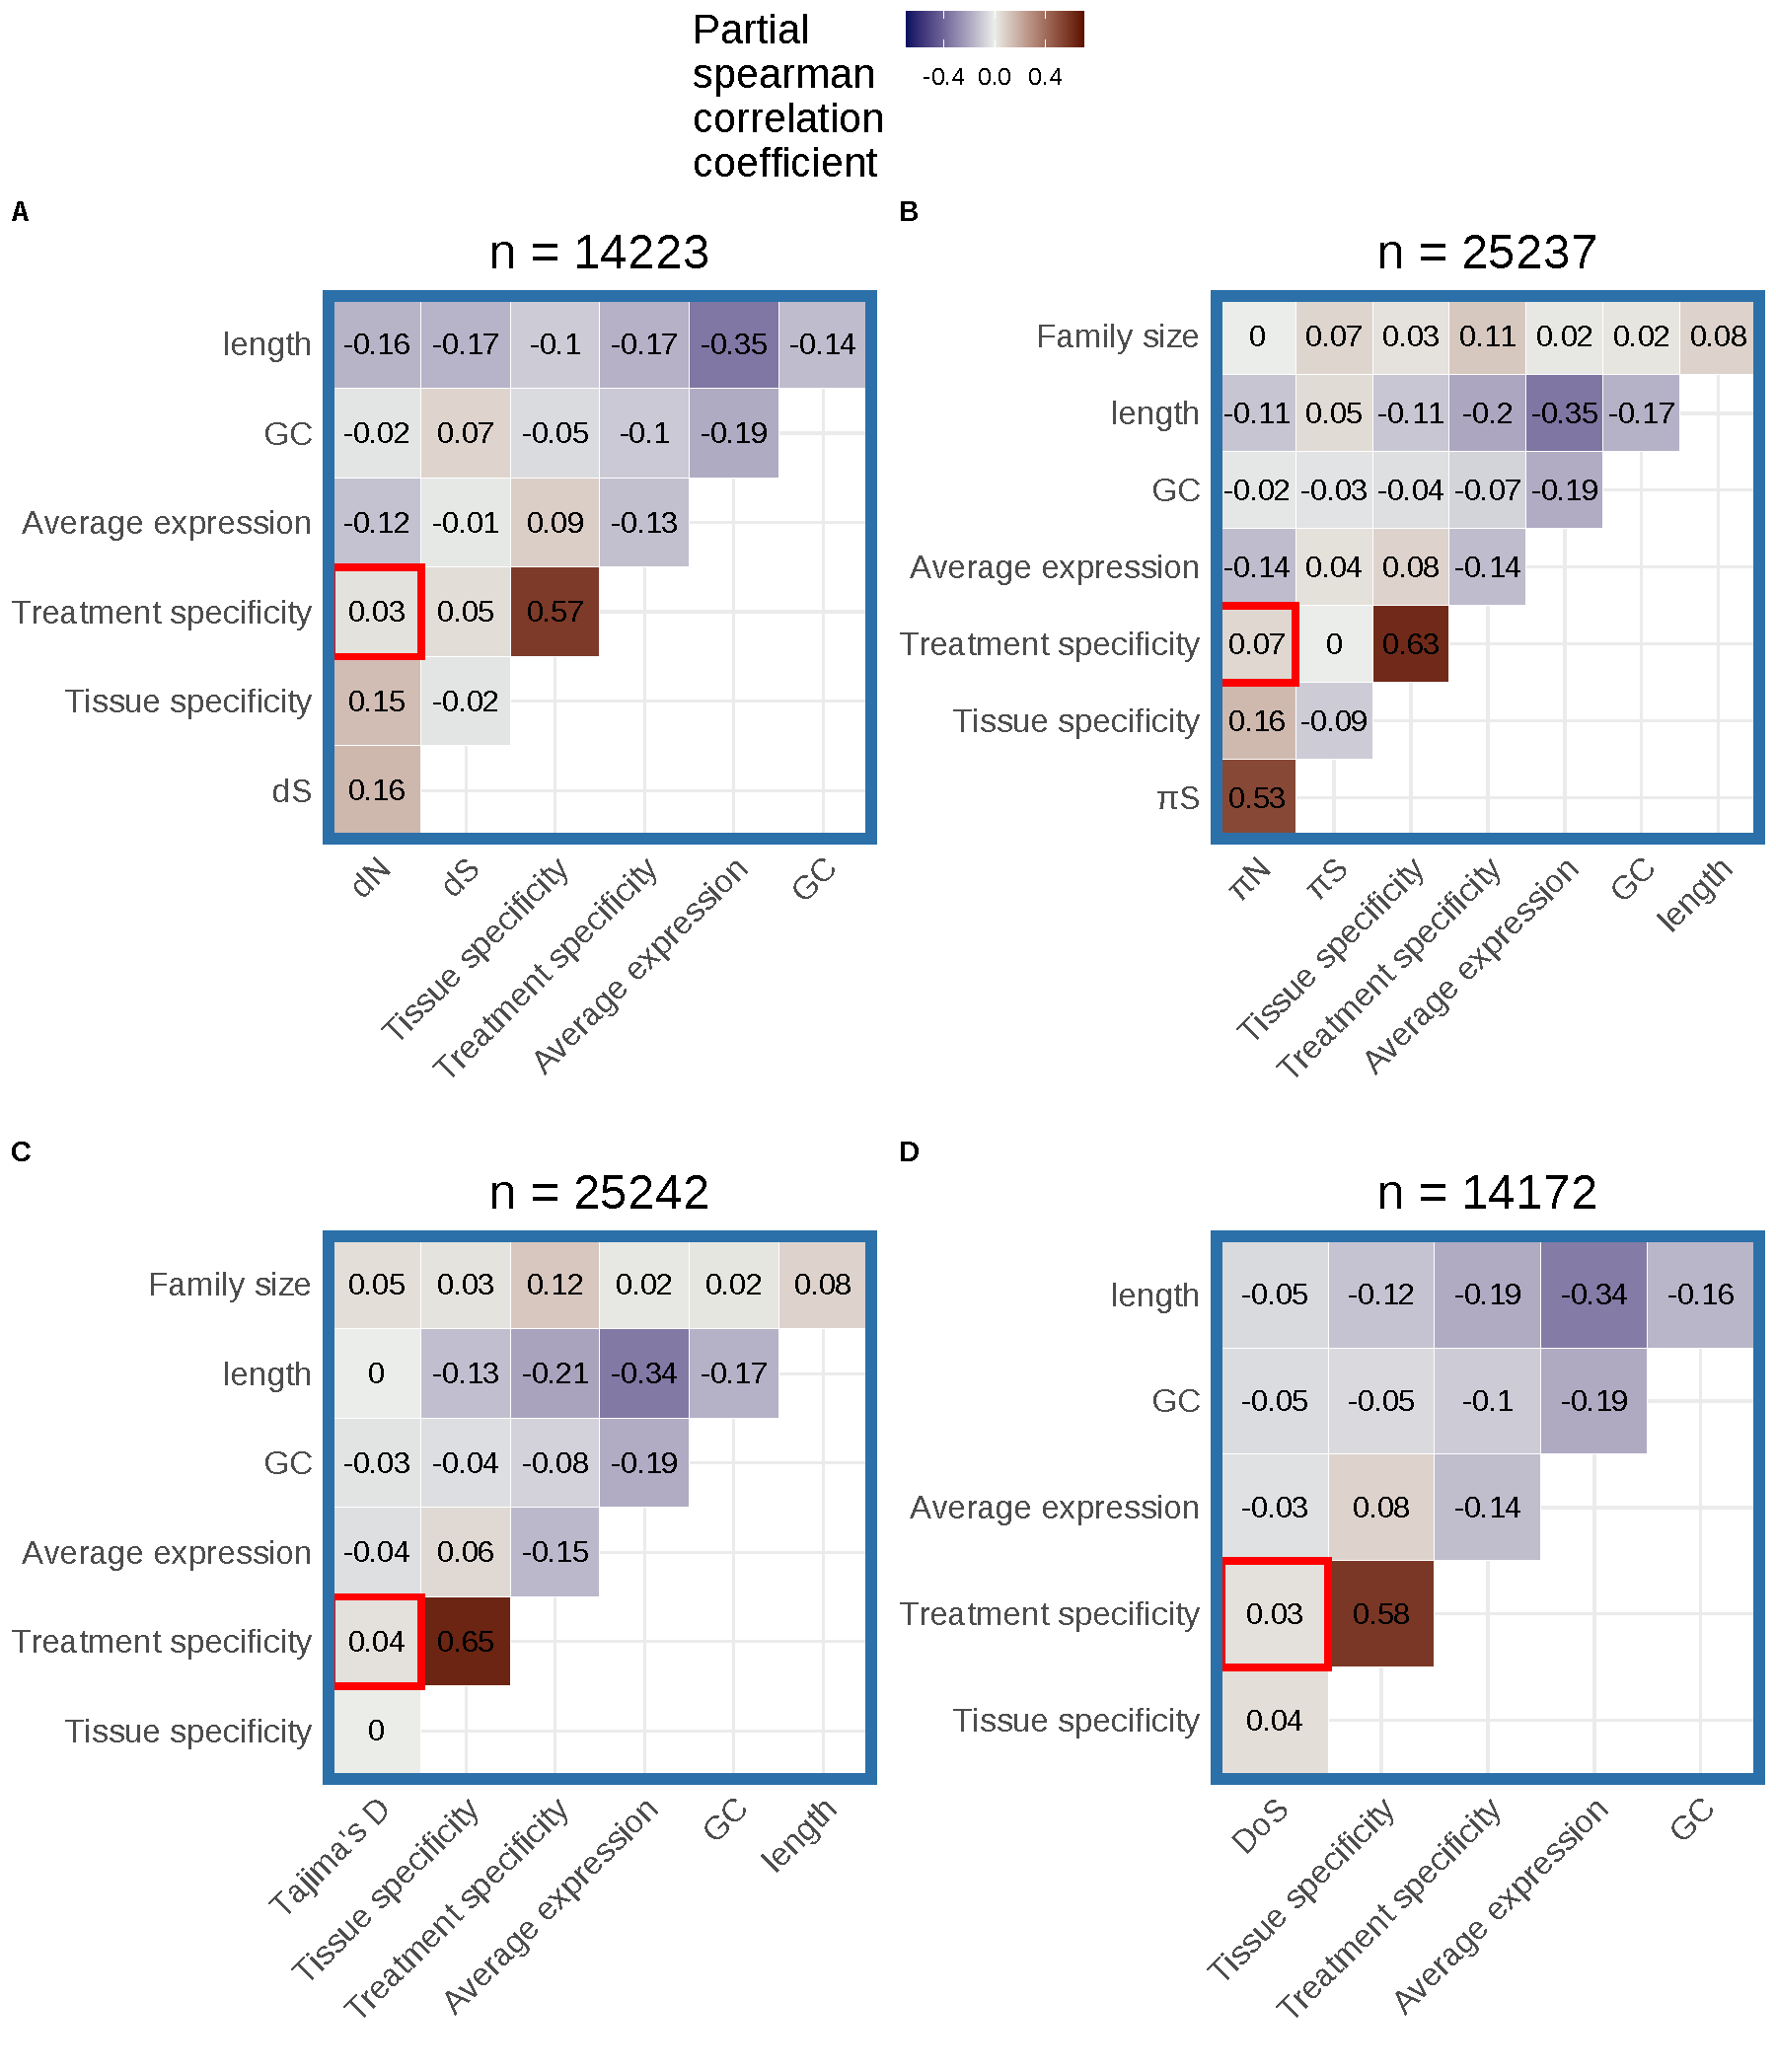
\includegraphics[width = \linewidth]{figures/appendix_a/partialCorrelations_withTissueSpecificity_seed_2023-02-20.pdf}
\caption{\textbf{Partial correlation analysis for seed tissue.} Partial correlations for (\textbf{A}) $dN$, (\textbf{B}) $\pi_N$, (\textbf{C}) Tajima's D, and (\textbf{D}) direction of selection (DoS) based on seed data. Average expression excludes values $<$ 5 TPM and was calculated using only seed tissue samples. Tissue-specificity was calculated using only control runs across all tissue categories. Treatment-specificity was calculated using only seed tissue runs. The number of genes included in each partial correlation analysis (n) is listed at the top of each heatmap.}%
\end{figure}

\newpage

\begin{figure}[H]
\centering
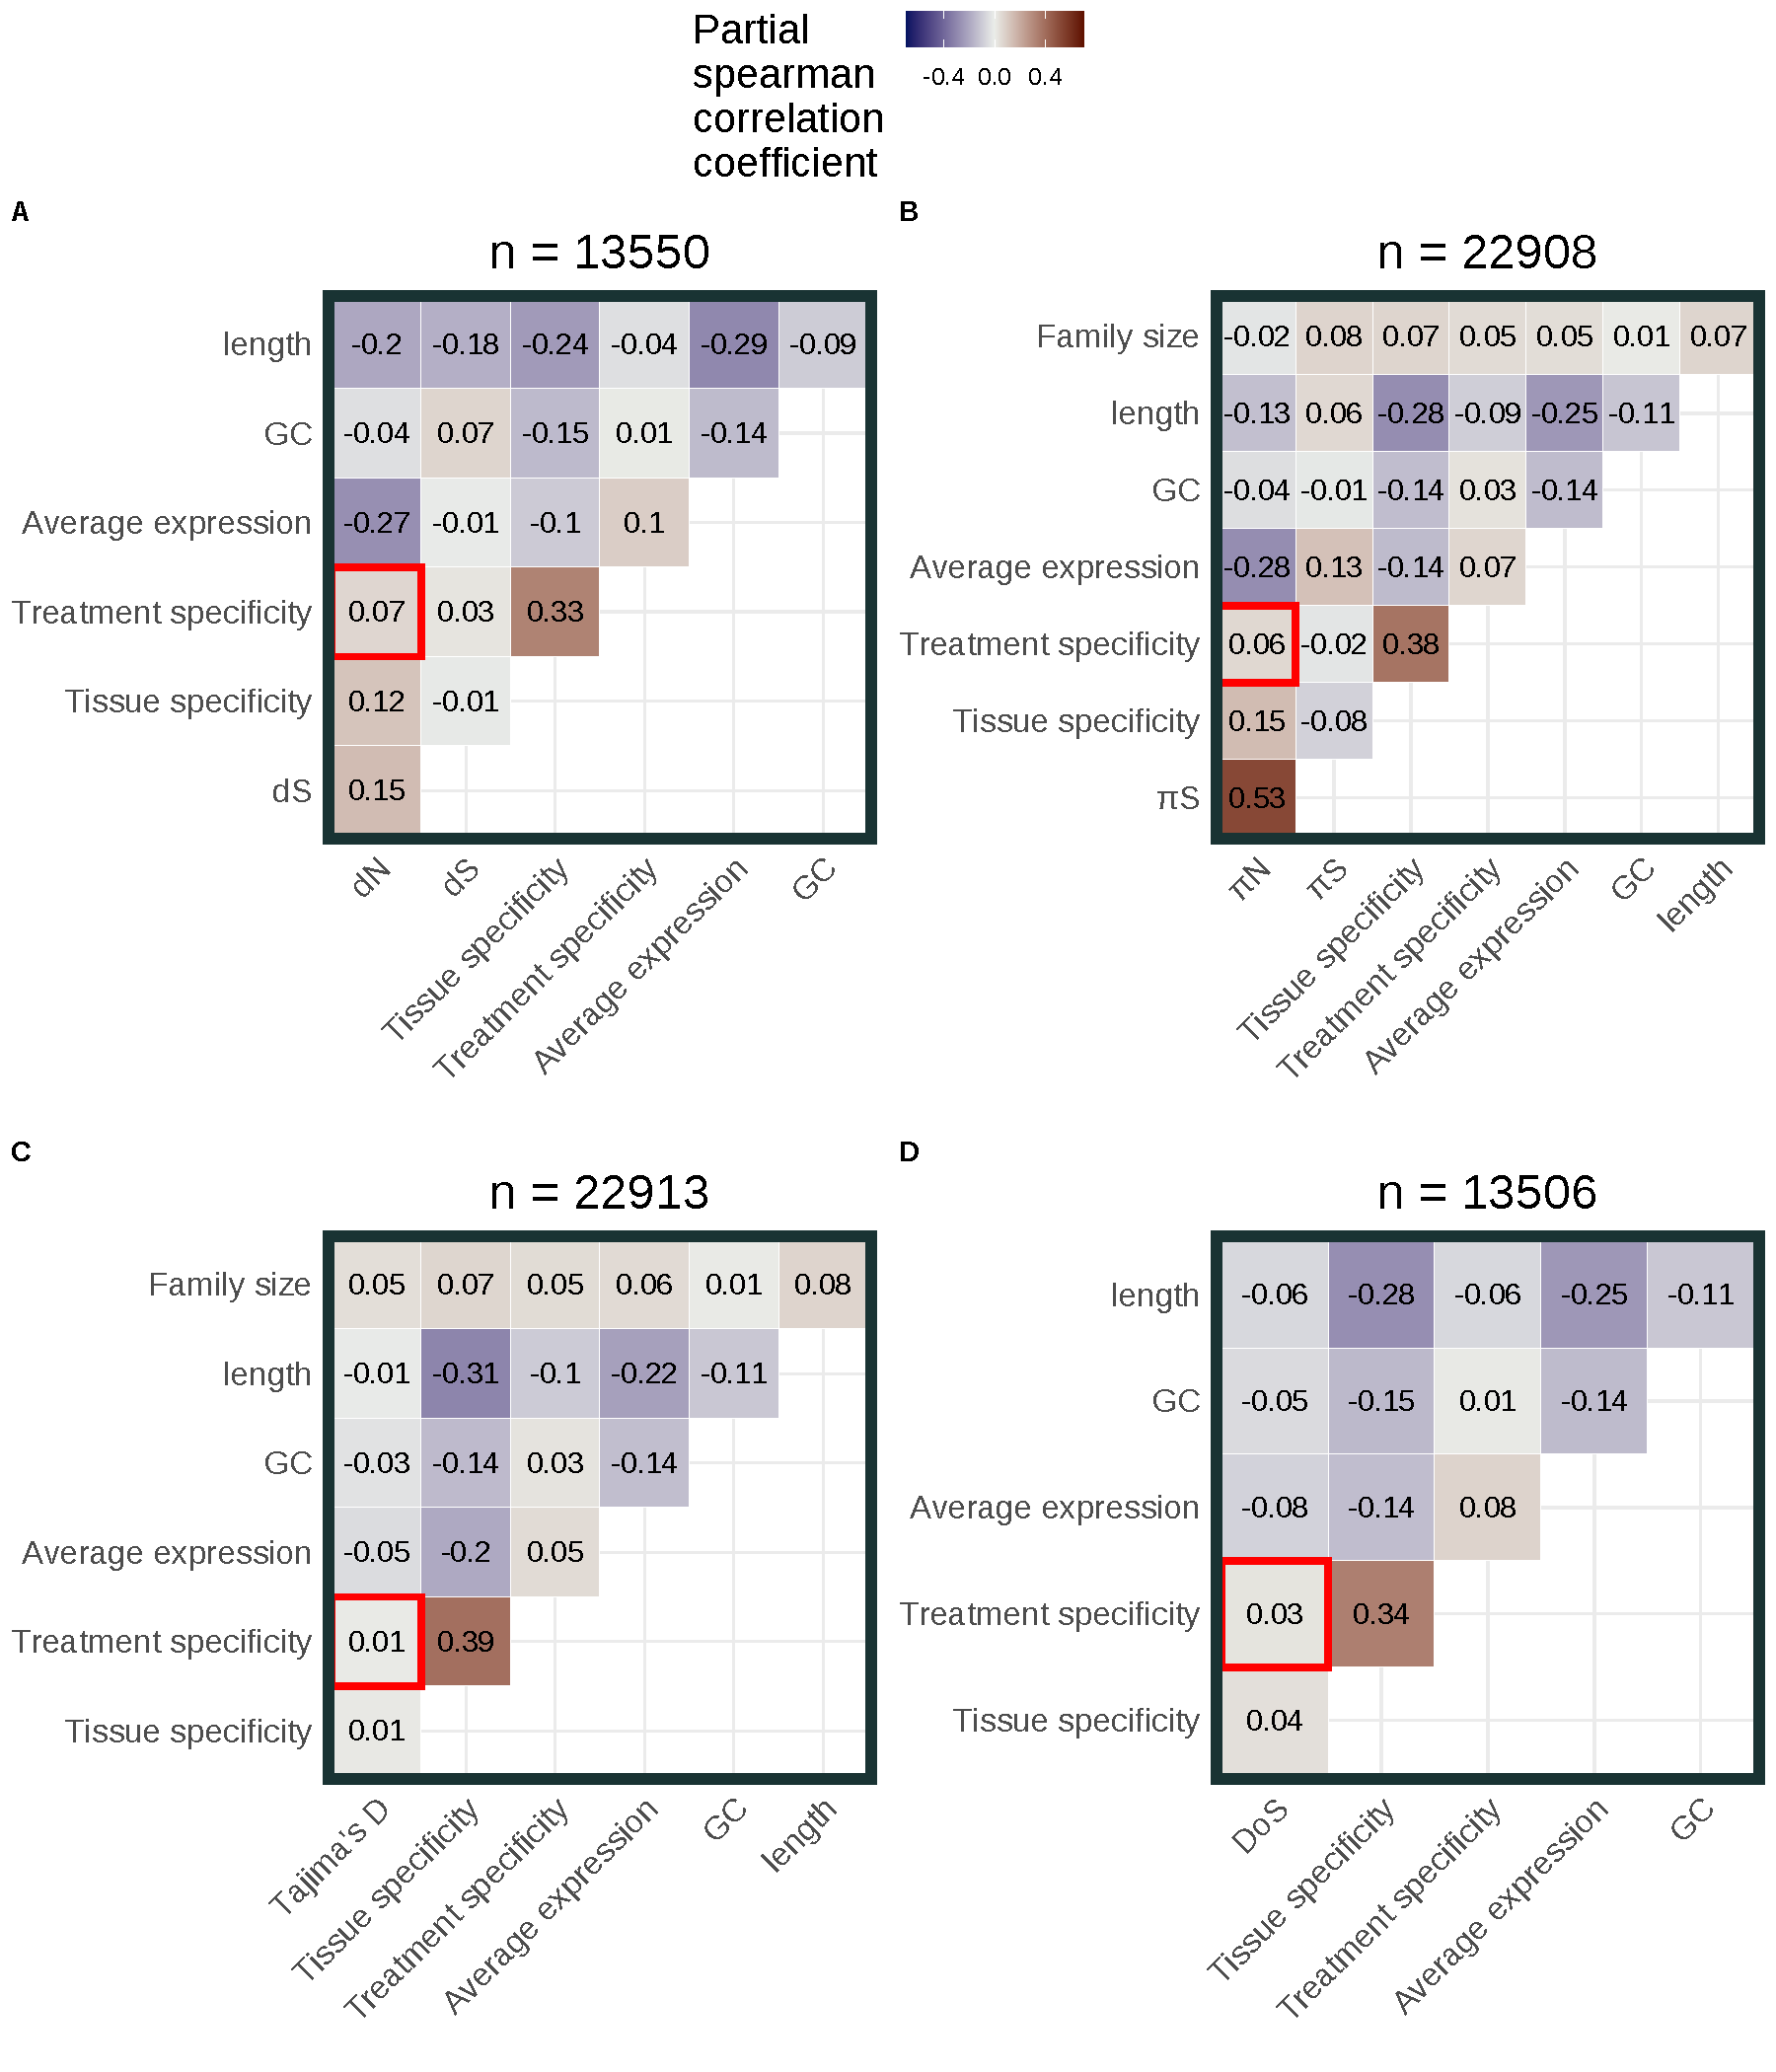
\includegraphics[width = \linewidth]{figures/appendix_a/partialCorrelations_withTissueSpecificity_fruitORflower_2023-02-20.pdf}
\caption{\textbf{Partial correlation analysis for fruit or flower tissue.} Partial correlations for (\textbf{A}) $dN$, (\textbf{B}) $\pi_N$, (\textbf{C}) Tajima's D, and (\textbf{D}) direction of selection (DoS) based on flower and fruit data. Average expression excludes values $<$ 5 TPM and was calculated using only fruit and flower tissue samples. Tissue-specificity was calculated using only control runs across all tissue categories. Treatment-specificity was calculated using only fruit and flower tissue runs. The number of genes included in each partial correlation analysis (n) is listed at the top of each heatmap.}%
\end{figure}

\subsection*{Partial correlations on data subset by tissue type after SVA}

\begin{figure}[H]
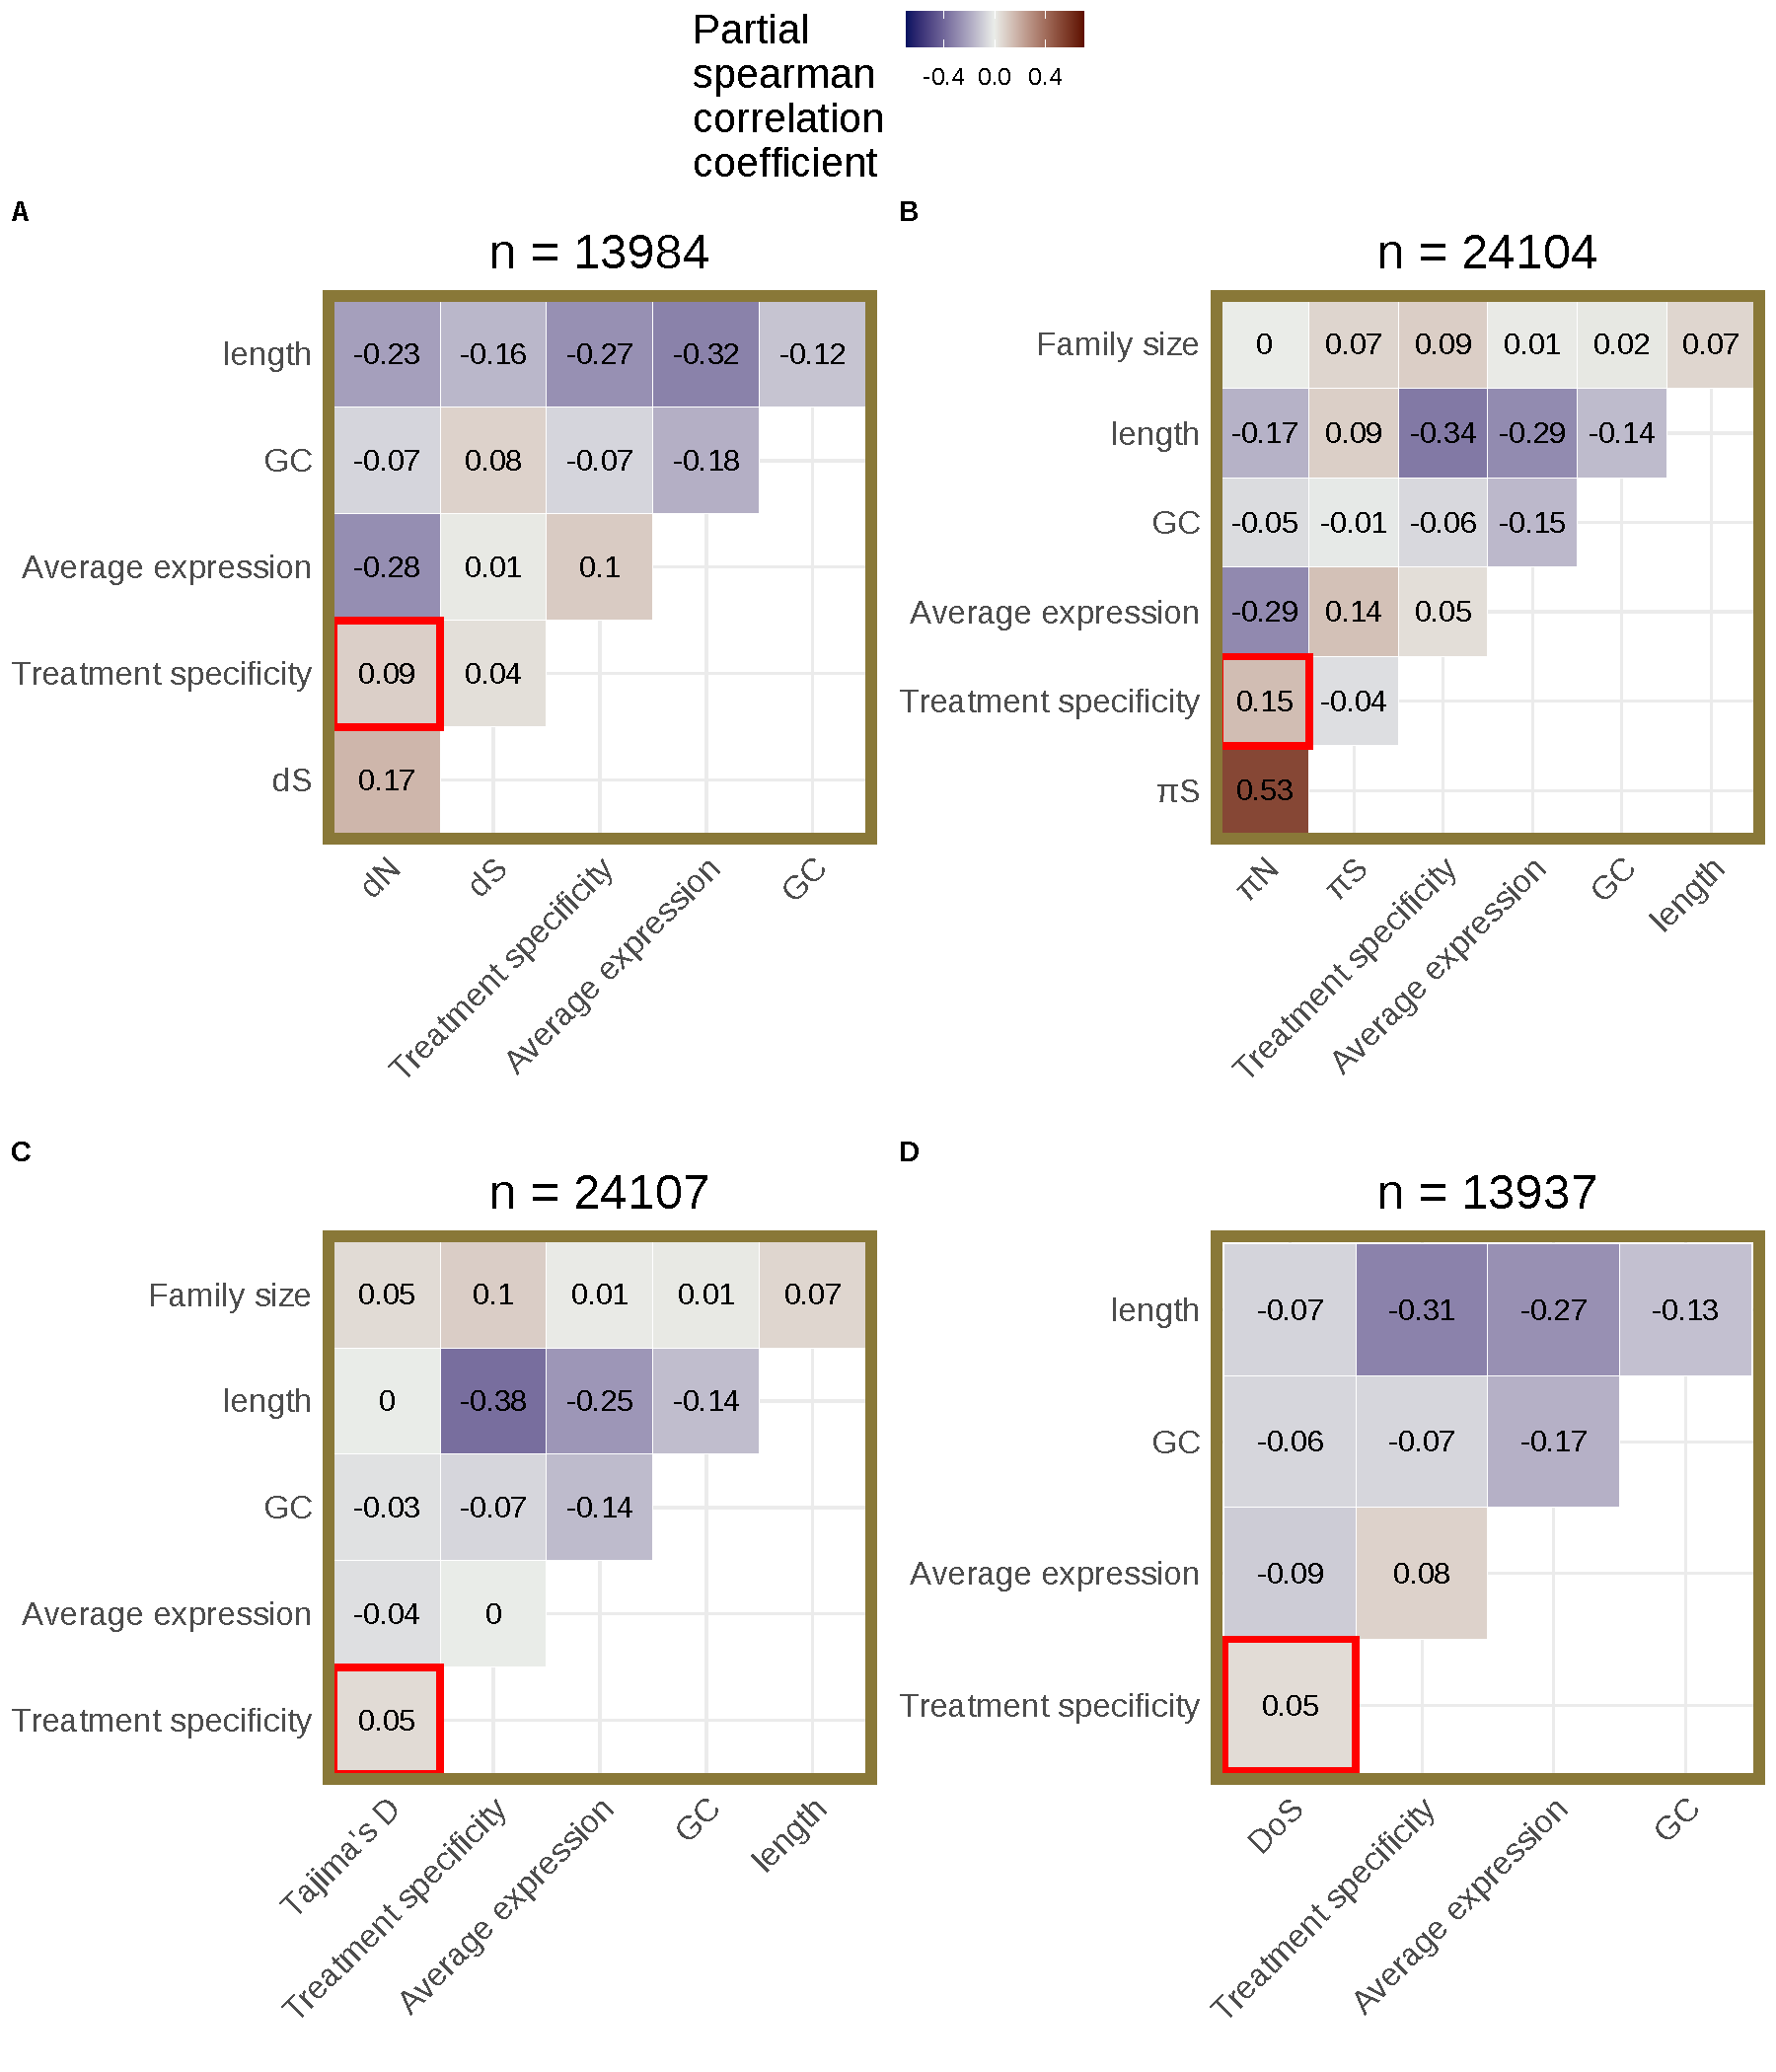
\includegraphics[width=\linewidth, height=\textheight, keepaspectratio]{figures/appendix_a/partialCorrelations_withoutTissueSpecificityAfterSVA_root_2023-02-21.pdf}
\caption{\textbf{Partial correlation analysis of root tissue after SVA.} Partial correlations for (\textbf{A}) $dN$, (\textbf{B}) $\pi_N$, (\textbf{C}) Tajima's D, and (\textbf{D}) direction of selection (DoS) based on root tissue data after applying SVA. Data was further subset to include only treatment groups with data from more than one study before applying SVA. The number of genes included in each partial correlation analysis (n) is listed at the top of each heatmap.}%
\end{figure}

\newpage

\begin{figure}[H]
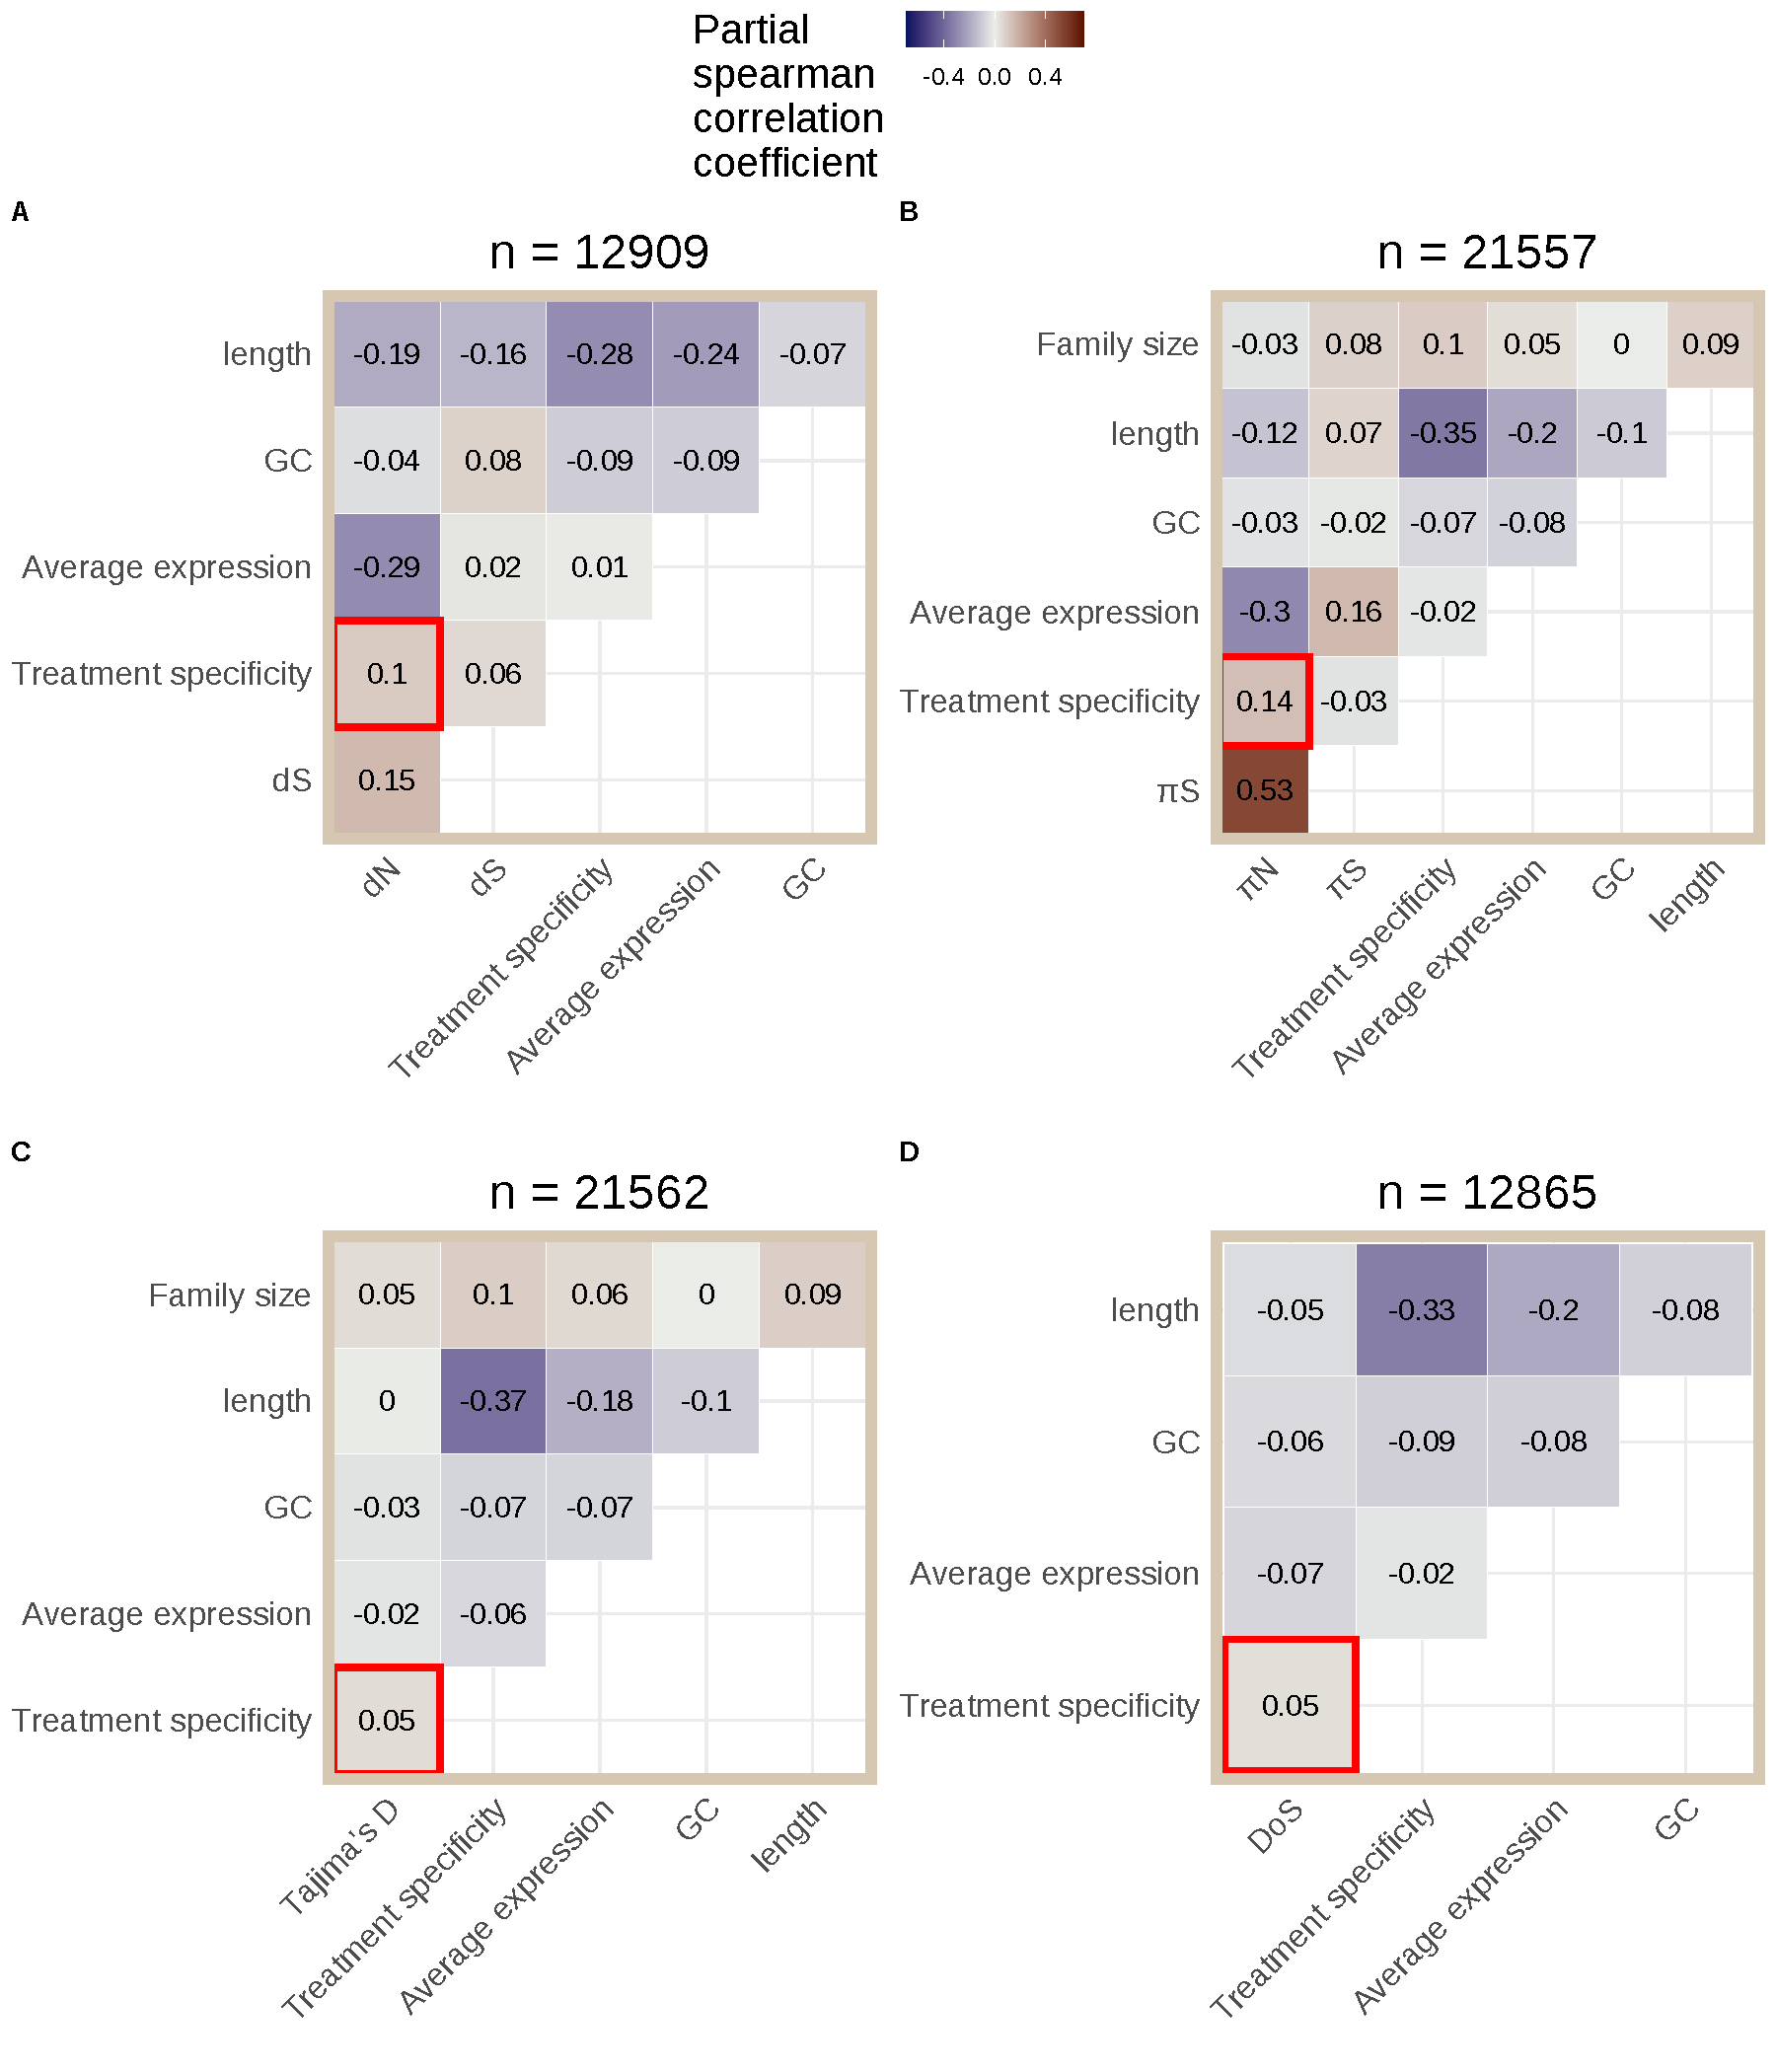
\includegraphics[width=\linewidth, height=\textheight, keepaspectratio]{figures/appendix_a/partialCorrelations_withoutTissueSpecificityAfterSVA_wholePlant_2023-02-21.pdf}
\caption{\textbf{Partial correlation analysis of whole plant tissue after SVA.} Partial correlations for (\textbf{A}) $dN$, (\textbf{B}) $\pi_N$, (\textbf{C}) Tajima's D, and (\textbf{D}) direction of selection (DoS) based on whole plant tissue data after applying SVA. Data was further subset to include only treatment groups with data from more than one study before applying SVA. The number of genes included in each partial correlation analysis (n) is listed at the top of each heatmap.}%
\end{figure}

\newpage

\begin{figure}[H]
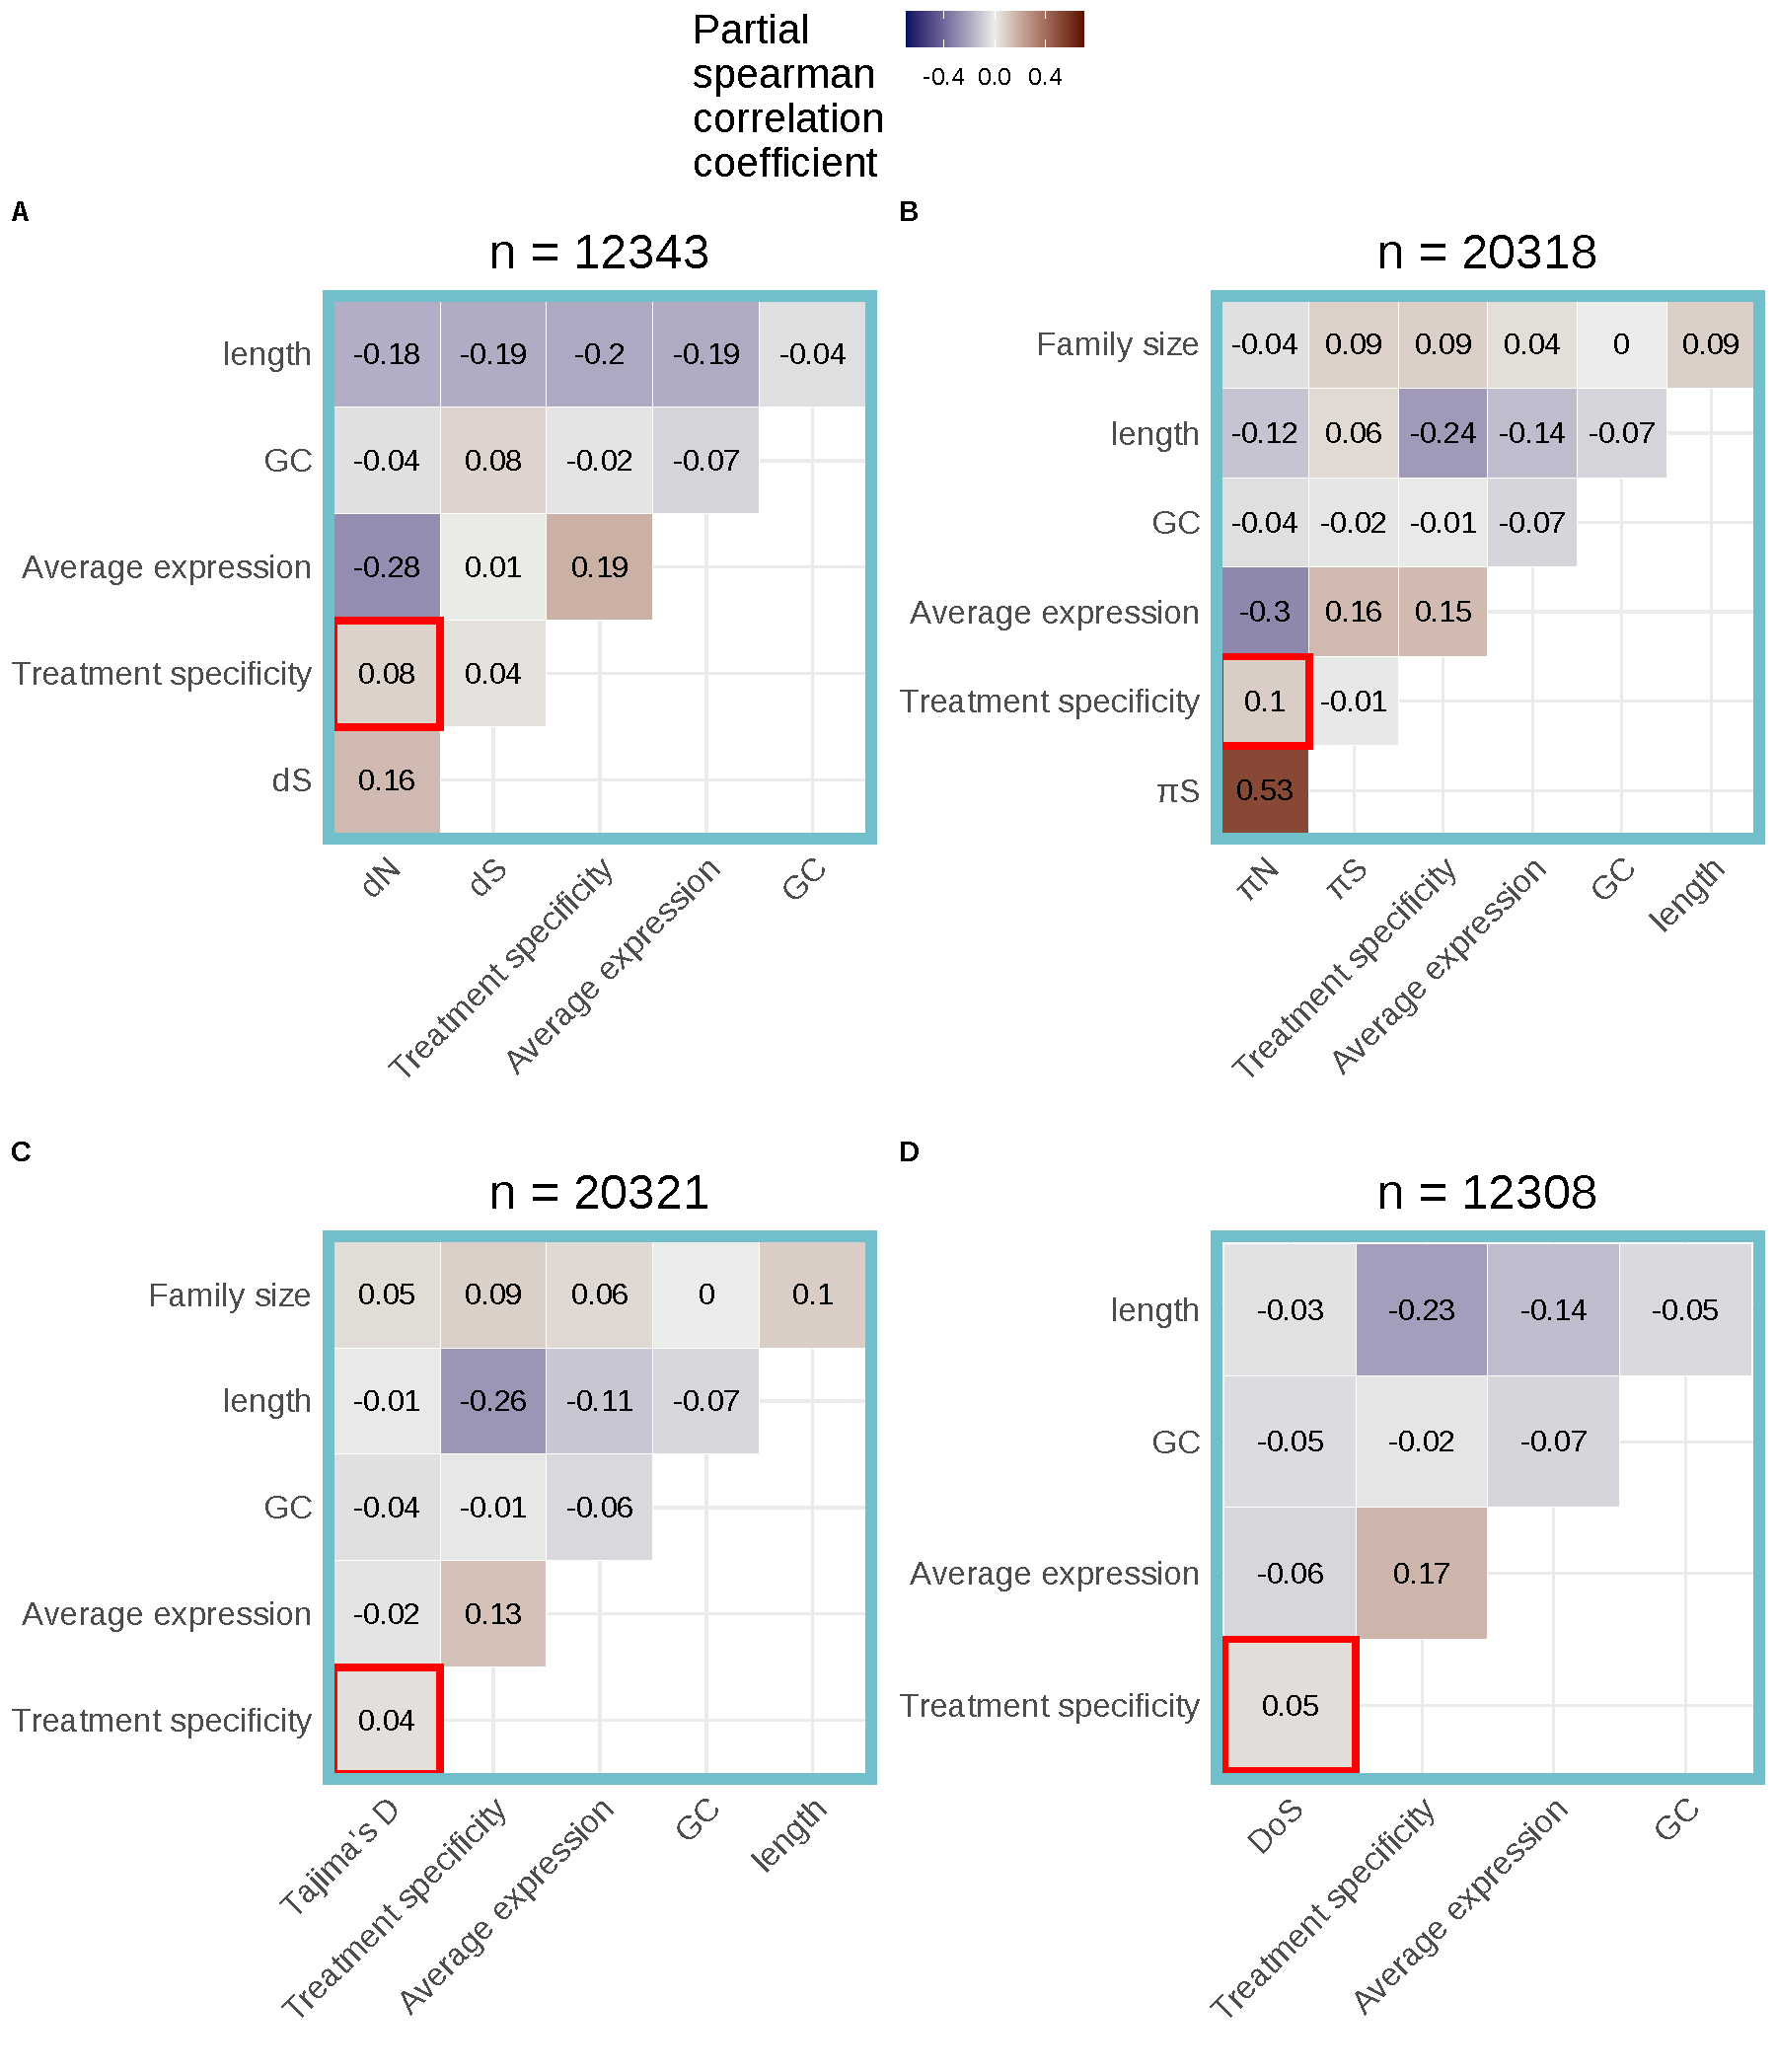
\includegraphics[width=\linewidth, height=\textheight, keepaspectratio]{figures/appendix_a/partialCorrelations_withoutTissueSpecificityAfterSVA_shoot_2023-02-21.pdf}
\caption{\textbf{Partial correlation analysis of shoot tissue after SVA.} Partial correlations for (\textbf{A}) $dN$, (\textbf{B}) $\pi_N$, (\textbf{C}) Tajima's D, and (\textbf{D}) direction of selection (DoS) based on shoot tissue data after applying SVA. Data was further subset to include only treatment groups with data from more than one study before applying SVA. The number of genes included in each partial correlation analysis (n) is listed at the top of each heatmap.}%
\end{figure}

\newpage

\begin{figure}[H]
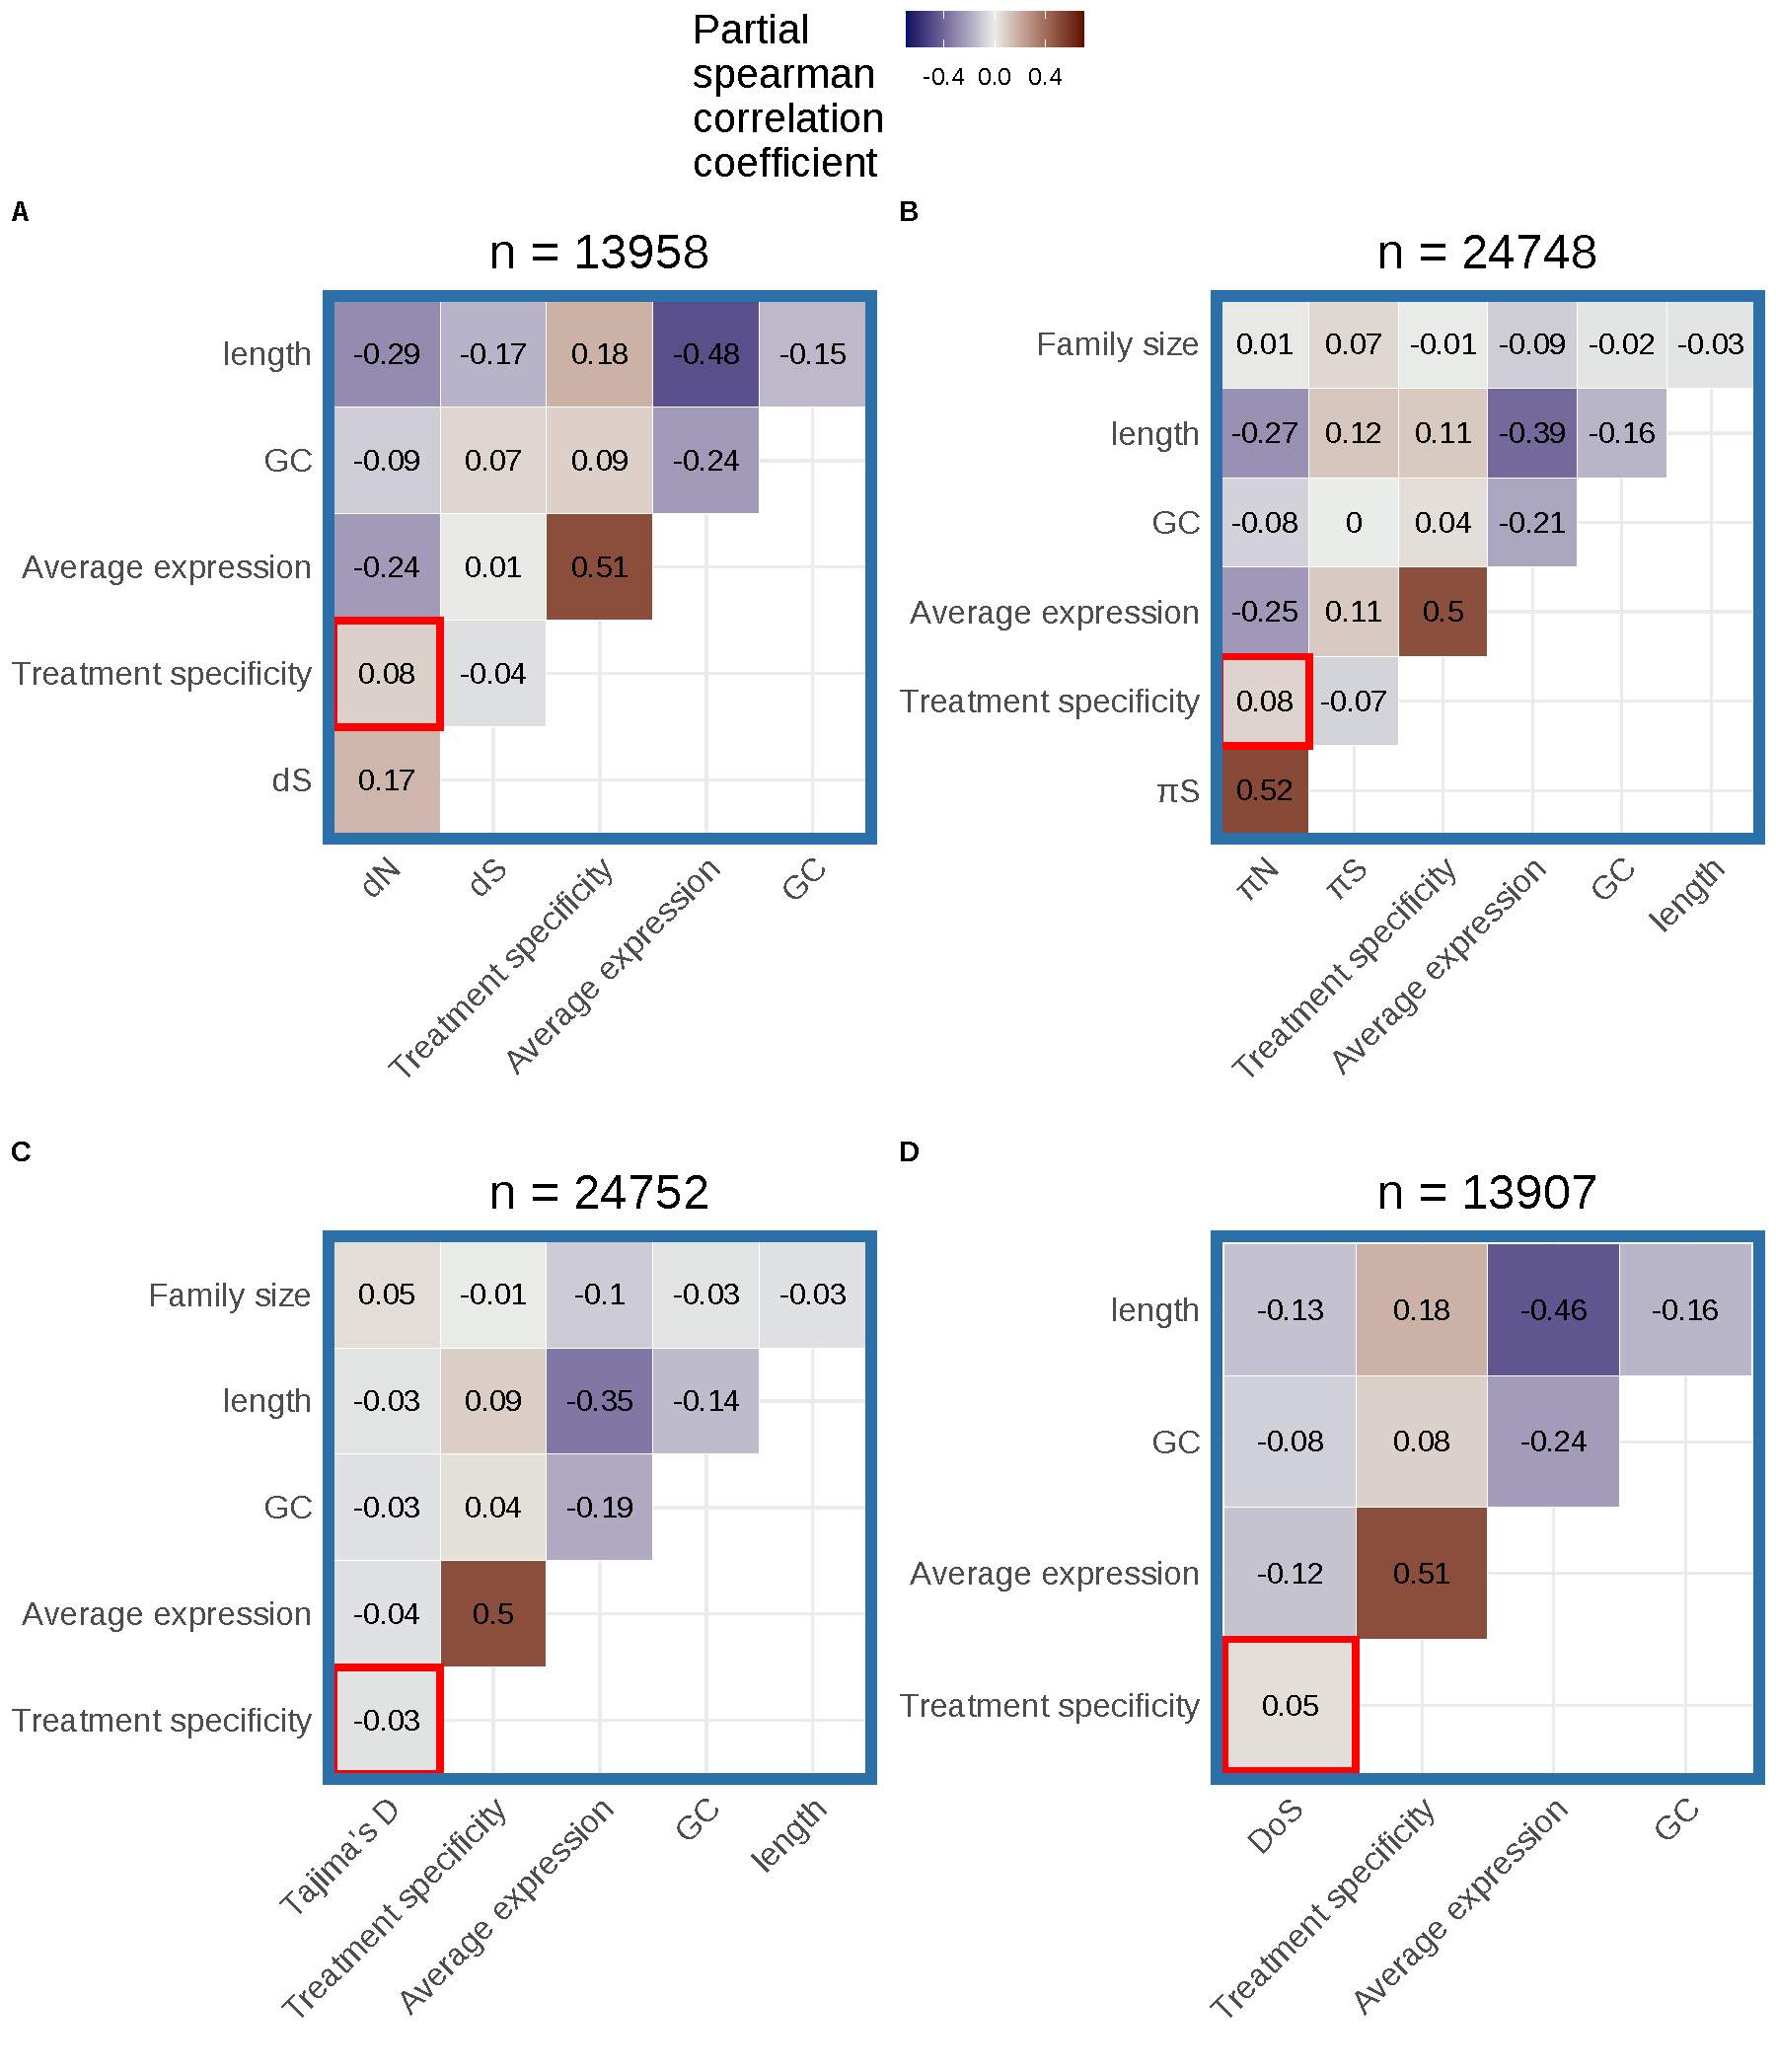
\includegraphics[width=\linewidth, height=\textheight, keepaspectratio]{figures/appendix_a/partialCorrelations_withoutTissueSpecificityAfterSVA_seed_2023-02-21.pdf}
\caption{\textbf{Partial correlation analysis of seed tissue after SVA.}Partial correlations for (\textbf{A}) $dN$, (\textbf{B}) $\pi_N$, (\textbf{C}) Tajima's D, and (\textbf{D}) direction of selection (DoS) based on seed tissue data after applying SVA. Data was further subset to include only treatment groups with data from more than one study before applying SVA. The number of genes included in each partial correlation analysis (n) is listed at the top of each heatmap.}%
\end{figure}

\newpage

\begin{figure}[H]
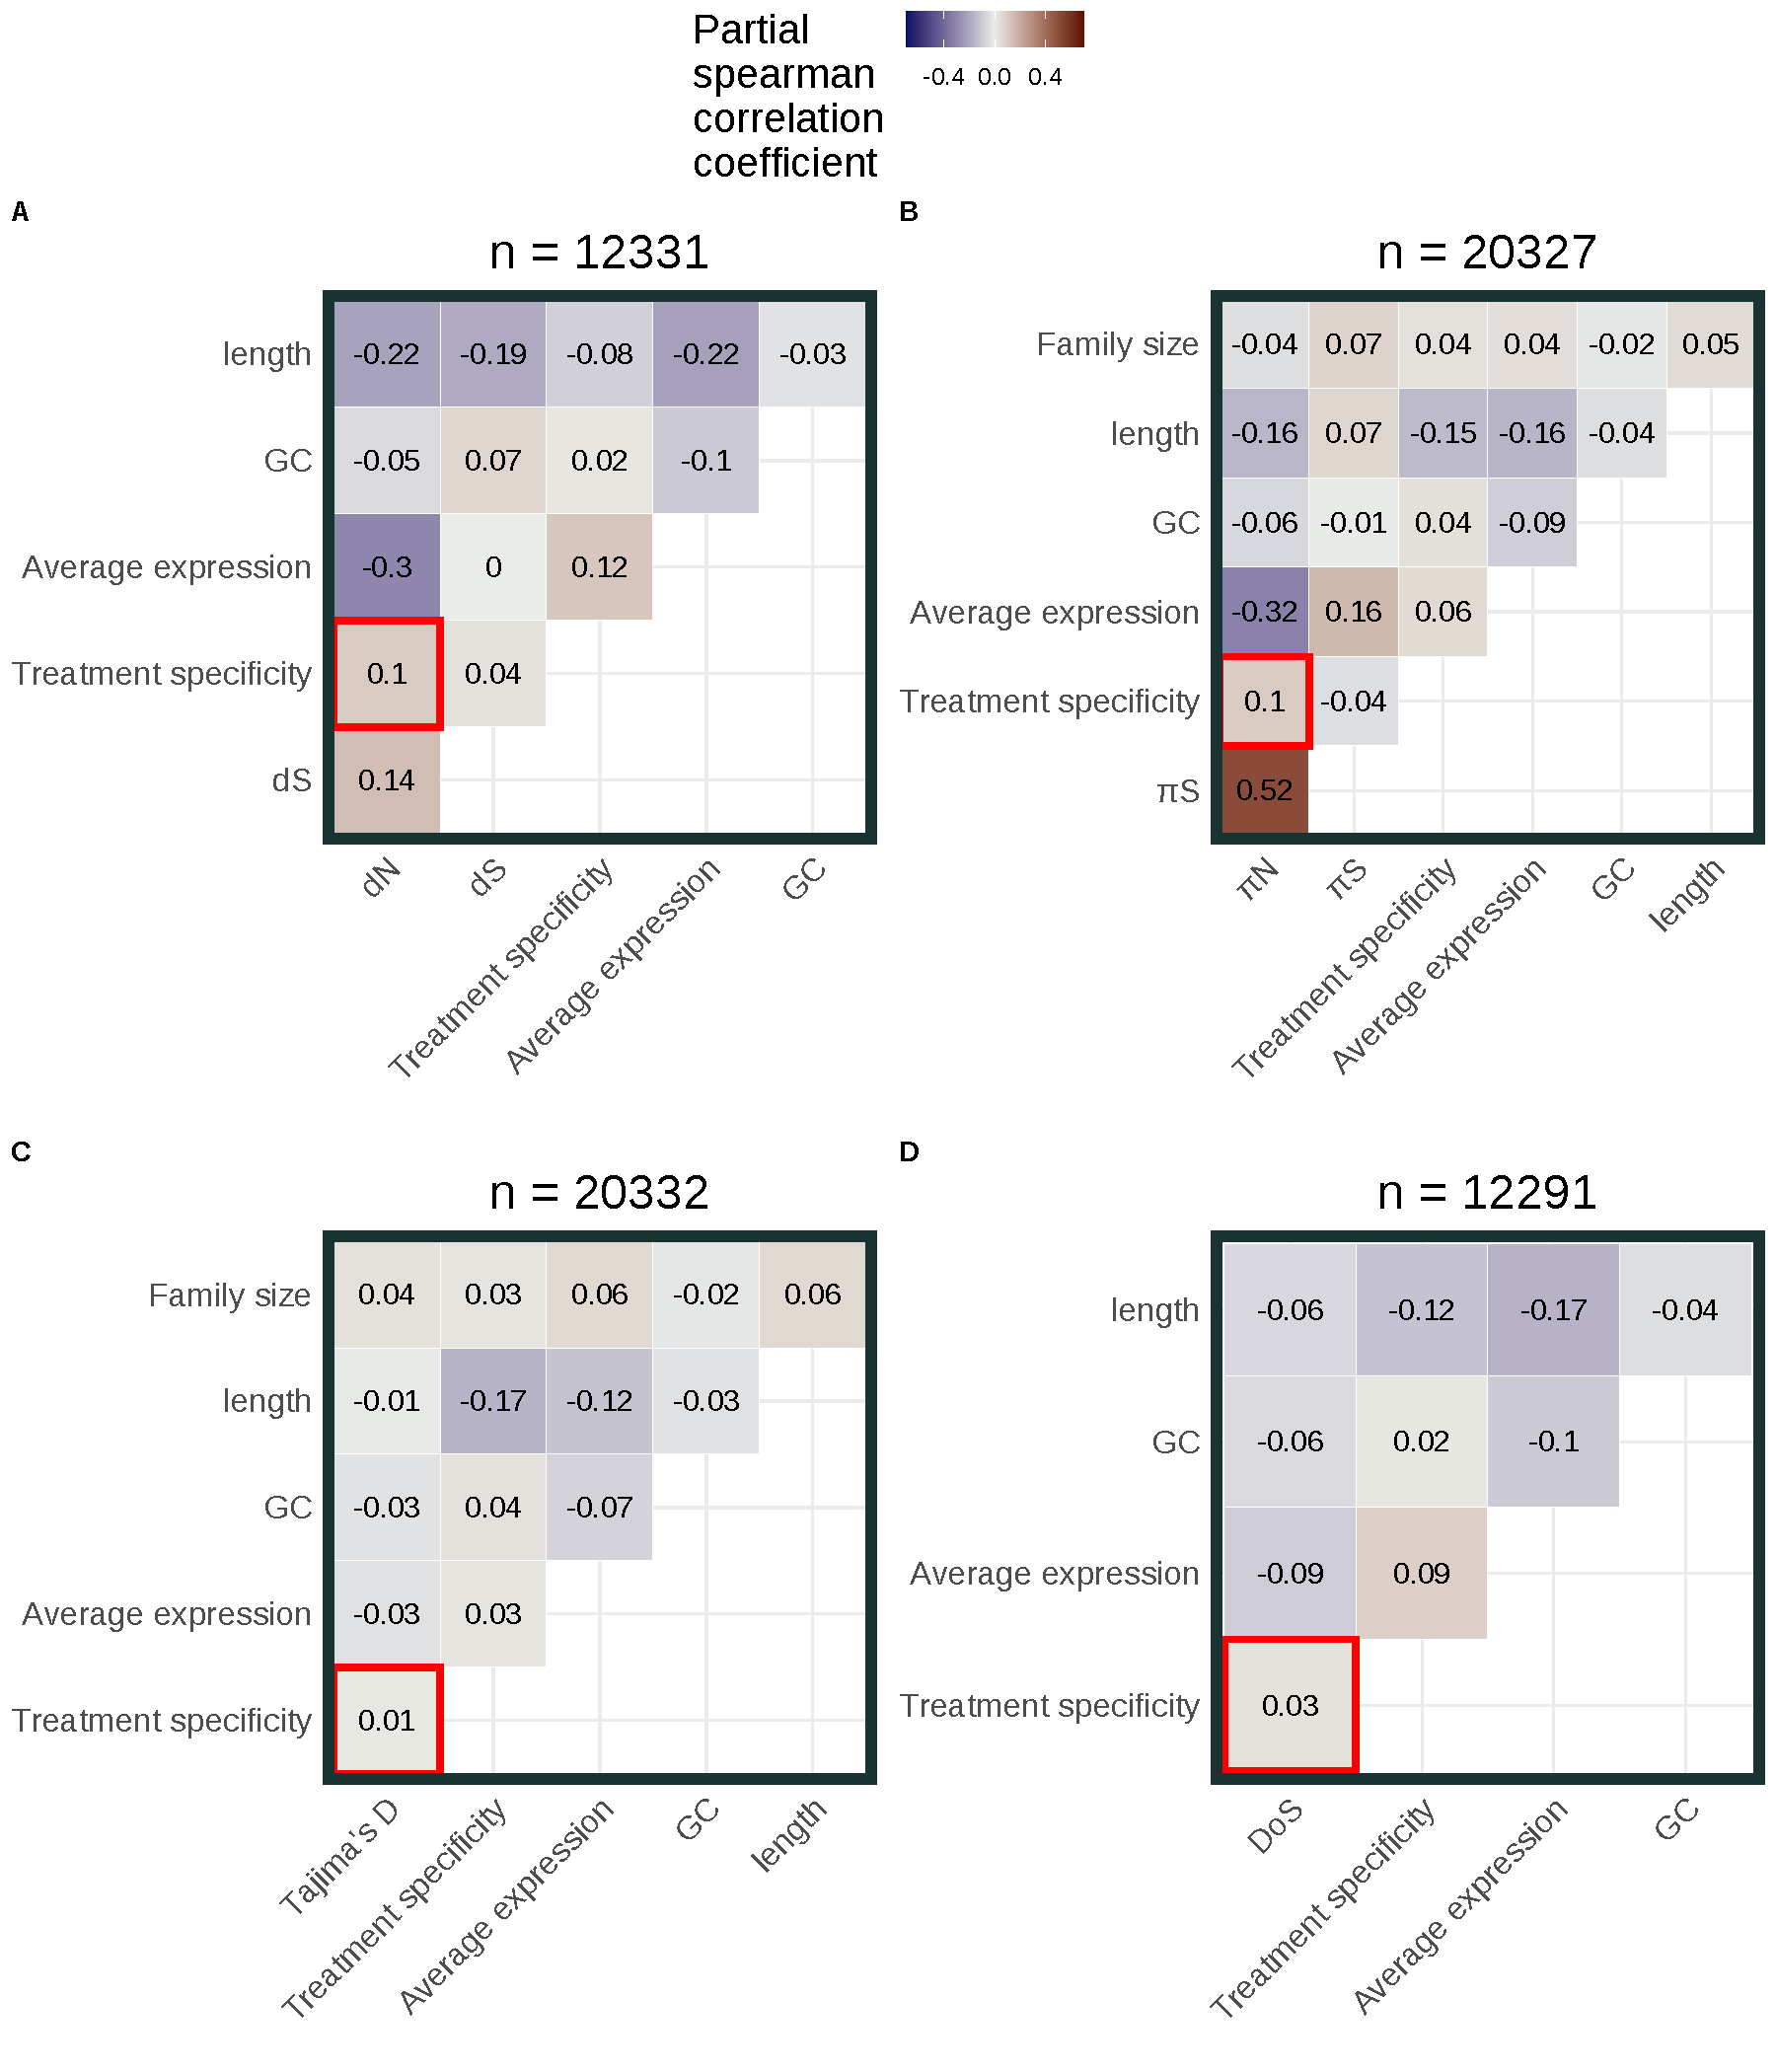
\includegraphics[width=\linewidth, height=\textheight, keepaspectratio]{figures/appendix_a/partialCorrelations_withoutTissueSpecificityAfterSVA_fruitORflower_2023-02-21.pdf}
\caption{\textbf{Partial correlation analysis of fruit or flower tissue after SVA.}Partial correlations for (\textbf{A}) $dN$, (\textbf{B}) $\pi_N$, (\textbf{C}) Tajima's D, and (\textbf{D}) direction of selection (DoS) based on flower and fruit tissue data after applying SVA. Data was further subset to include only treatment groups with data from more than one study before applying SVA. The number of genes included in each partial correlation analysis (n) is listed at the top of each heatmap.}%
\end{figure}

\subsection*{PCA before and after SVA on data subset by tissue type} 

\begin{figure}[H]
\centering
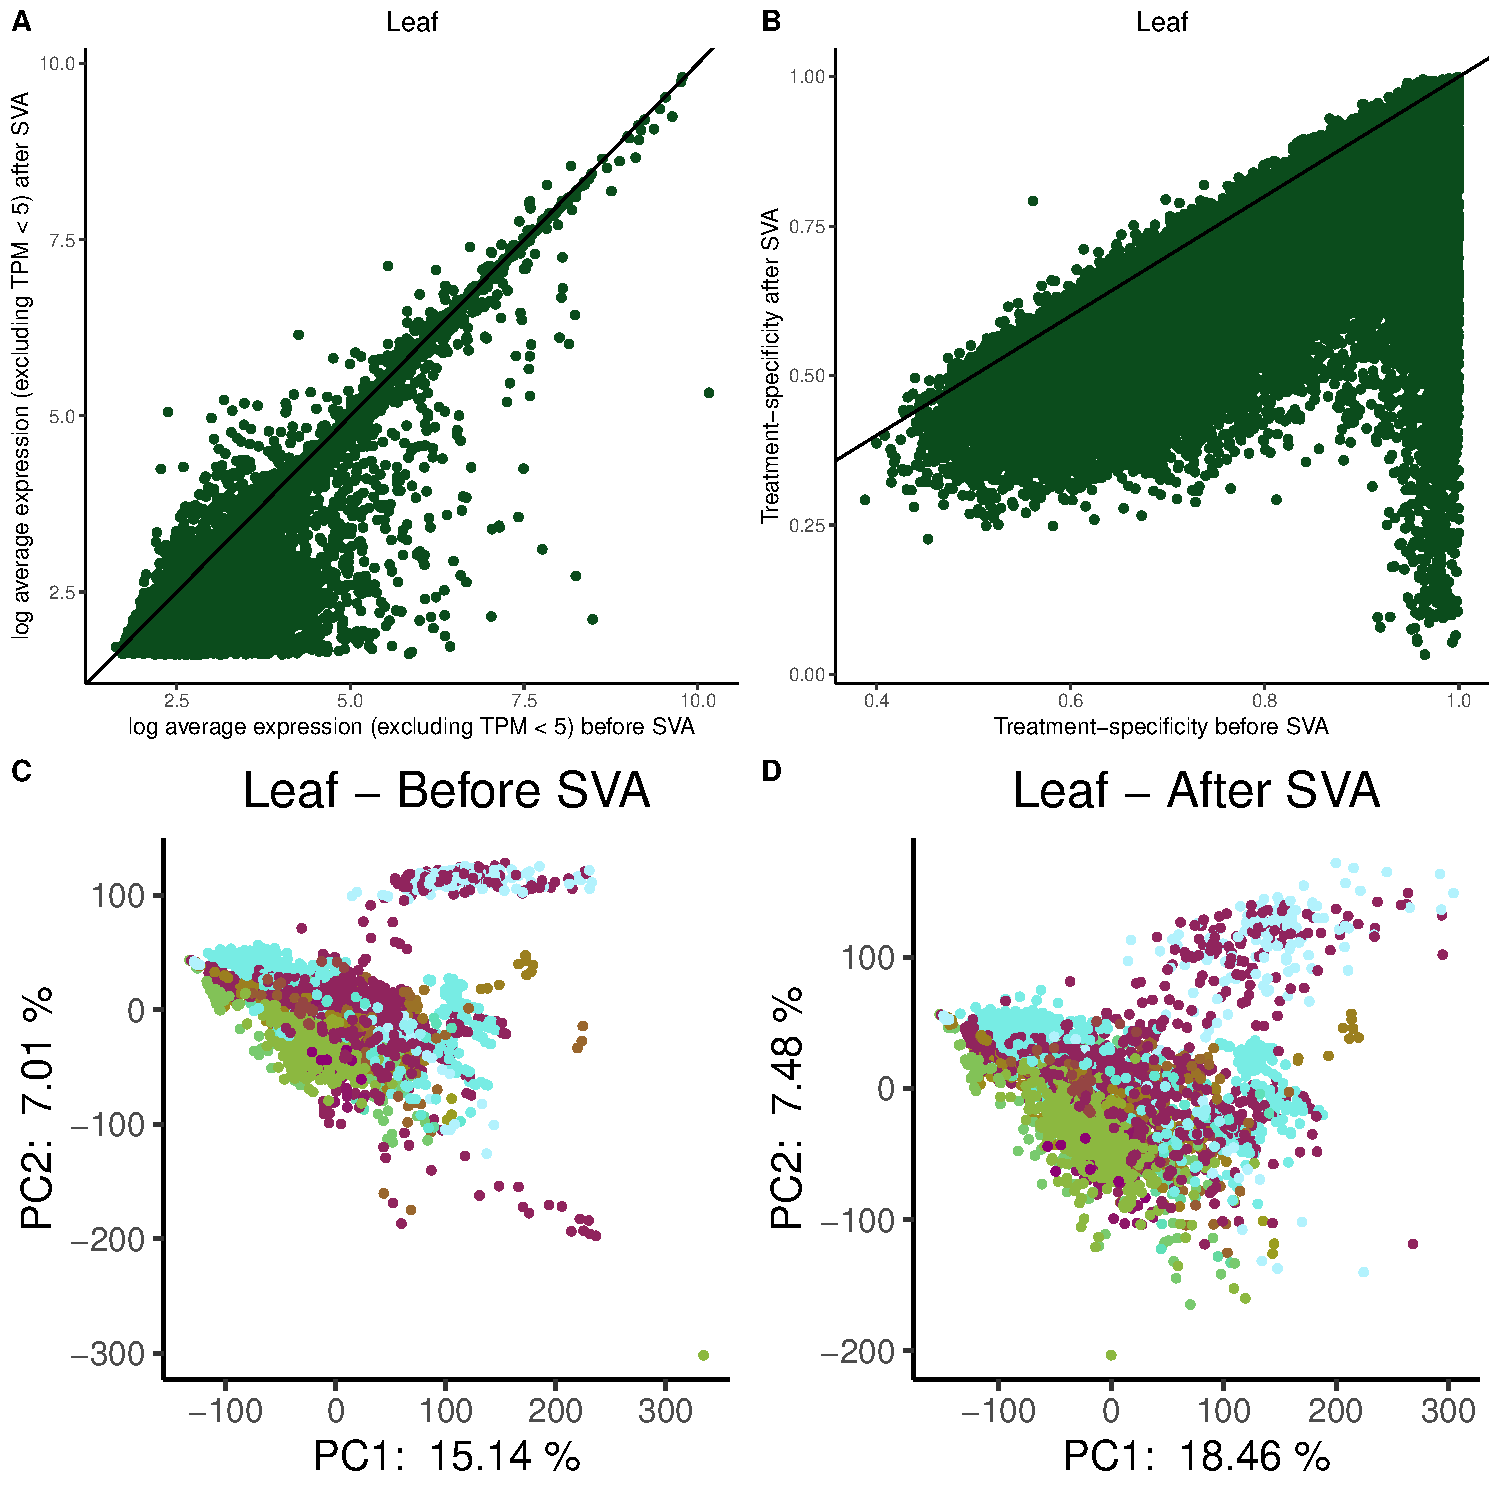
\includegraphics[width = \linewidth]{figures/appendix_a/pca_beforeAndAfterSva_leaf_2023-02-21.pdf}
\caption{\textbf{Effect of surrogate variable analysis on structure of leaf tissue data.} (\textbf{A}) Effect of SVA on average expression. (\textbf{B}) Effect of SVA on treatment-specificity. (\textbf{C}) Principal component analysis of leaf tissue data before SVA. (\textbf{D}) Principal component analysis of leaf tissue data after SVA. Color in the PCA plots represent different experimental treatments - legend is Figure \ref{fig::pcaLegendLeaf}.}%
\end{figure}

\begin{figure}[H]
\centering
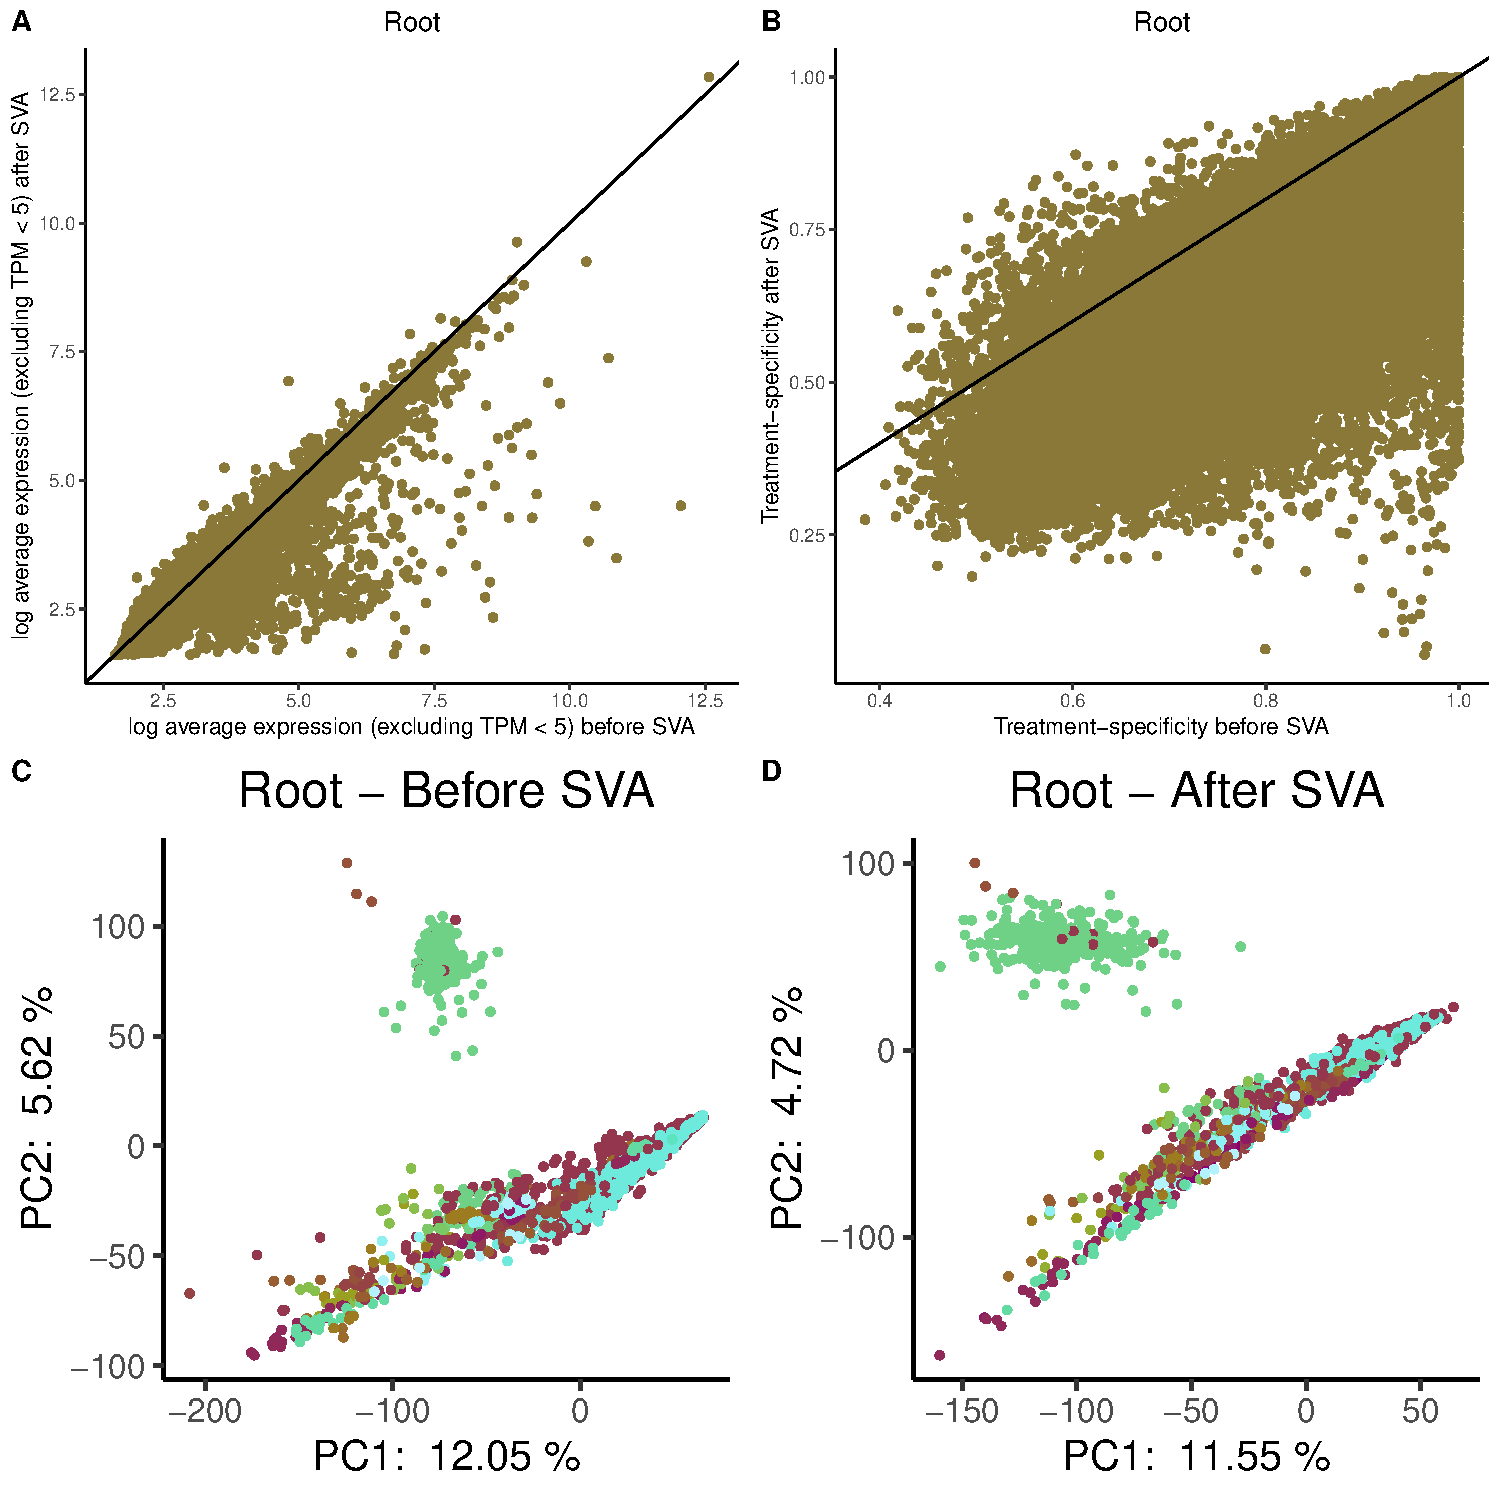
\includegraphics[width = \linewidth]{figures/appendix_a/pca_beforeAndAfterSva_root_2023-02-21.pdf}
\caption{\textbf{Effect of surrogate variable analysis on structure of root tissue data.} (\textbf{A}) Effect of SVA on average expression. (\textbf{B}) Effect of SVA on treatment-specificity. (\textbf{C}) Principal component analysis of root tissue data before SVA. (\textbf{D}) Principal component analysis of root tissue data after SVA.Color in the PCA plots represent different experimental treatments - legend is Figure \ref{fig::pcaLegendRoot}.}%
\end{figure}

\begin{figure}[H]
\centering
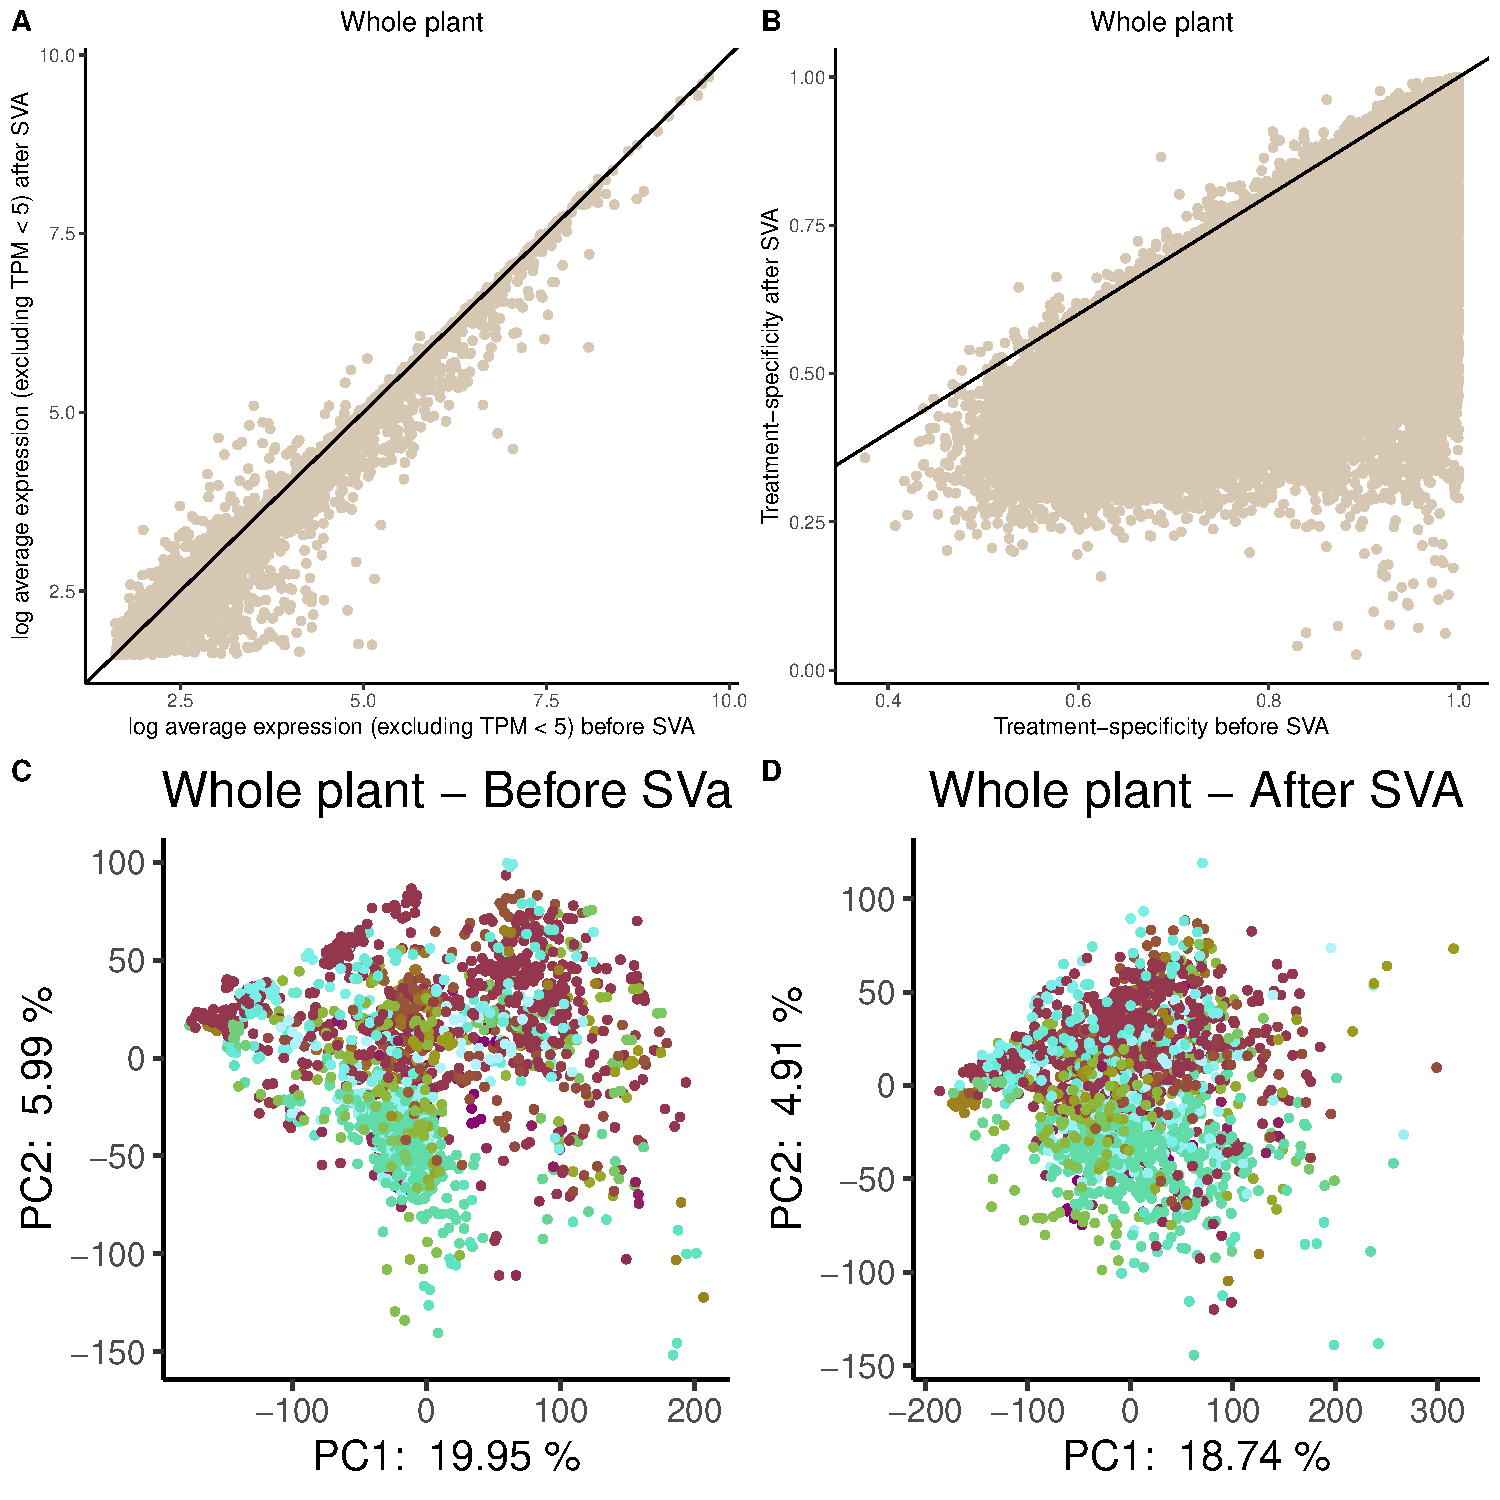
\includegraphics[width = \linewidth]{figures/appendix_a/pca_beforeAndAfterSva_plant_2023-02-21.pdf}
\caption{\textbf{Effect of surrogate variable analysis on structure of whole plant tissue data.} (\textbf{A}) Effect of SVA on average expression. (\textbf{B}) Effect of SVA on treatment-specificity. (\textbf{C}) Principal component analysis of whole plant tissue data before SVA. (\textbf{D}) Principal component analysis of whole plant tissue data after SVA.Color in the PCA plots represent different experimental treatments - legend is Figure \ref{fig::pcaLegendPlant}.}%
\end{figure}

\begin{figure}[H]
\centering
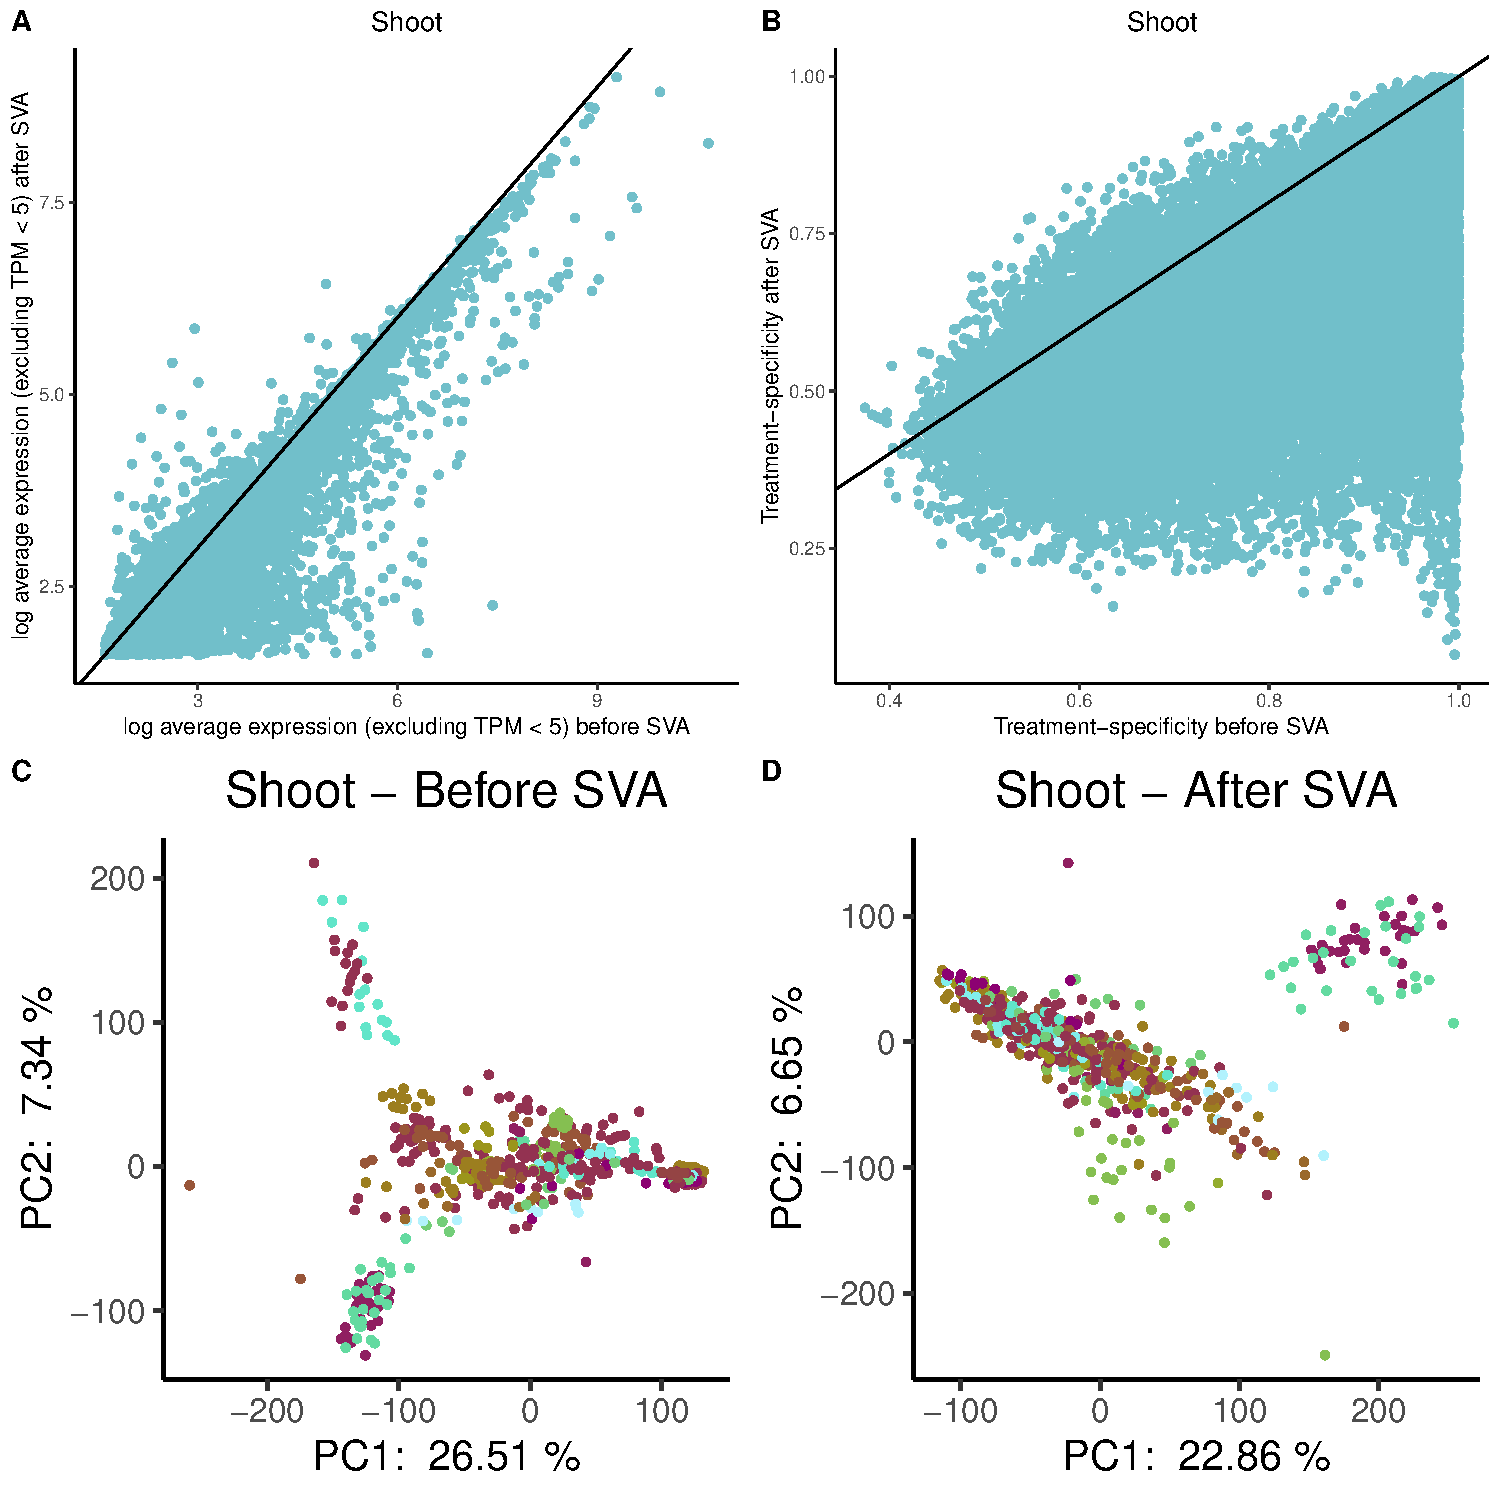
\includegraphics[width = \linewidth]{figures/appendix_a/pca_beforeAndAfterSva_shoot_2023-02-21.pdf}
\caption{\textbf{Effect of surrogate variable analysis on structure of shoot tissue data.} (\textbf{A}) Effect of SVA on average expression. (\textbf{B}) Effect of SVA on treatment-specificity. (\textbf{C}) Principal component analysis of shoot tissue data before SVA. (\textbf{D}) Principal component analysis of shoot tissue data after SVA. Color in the PCA plots represent different experimental treatments - legend is Figure \ref{fig::pcaLegendShoot}.}%
\end{figure}

\begin{figure}[H]
\centering
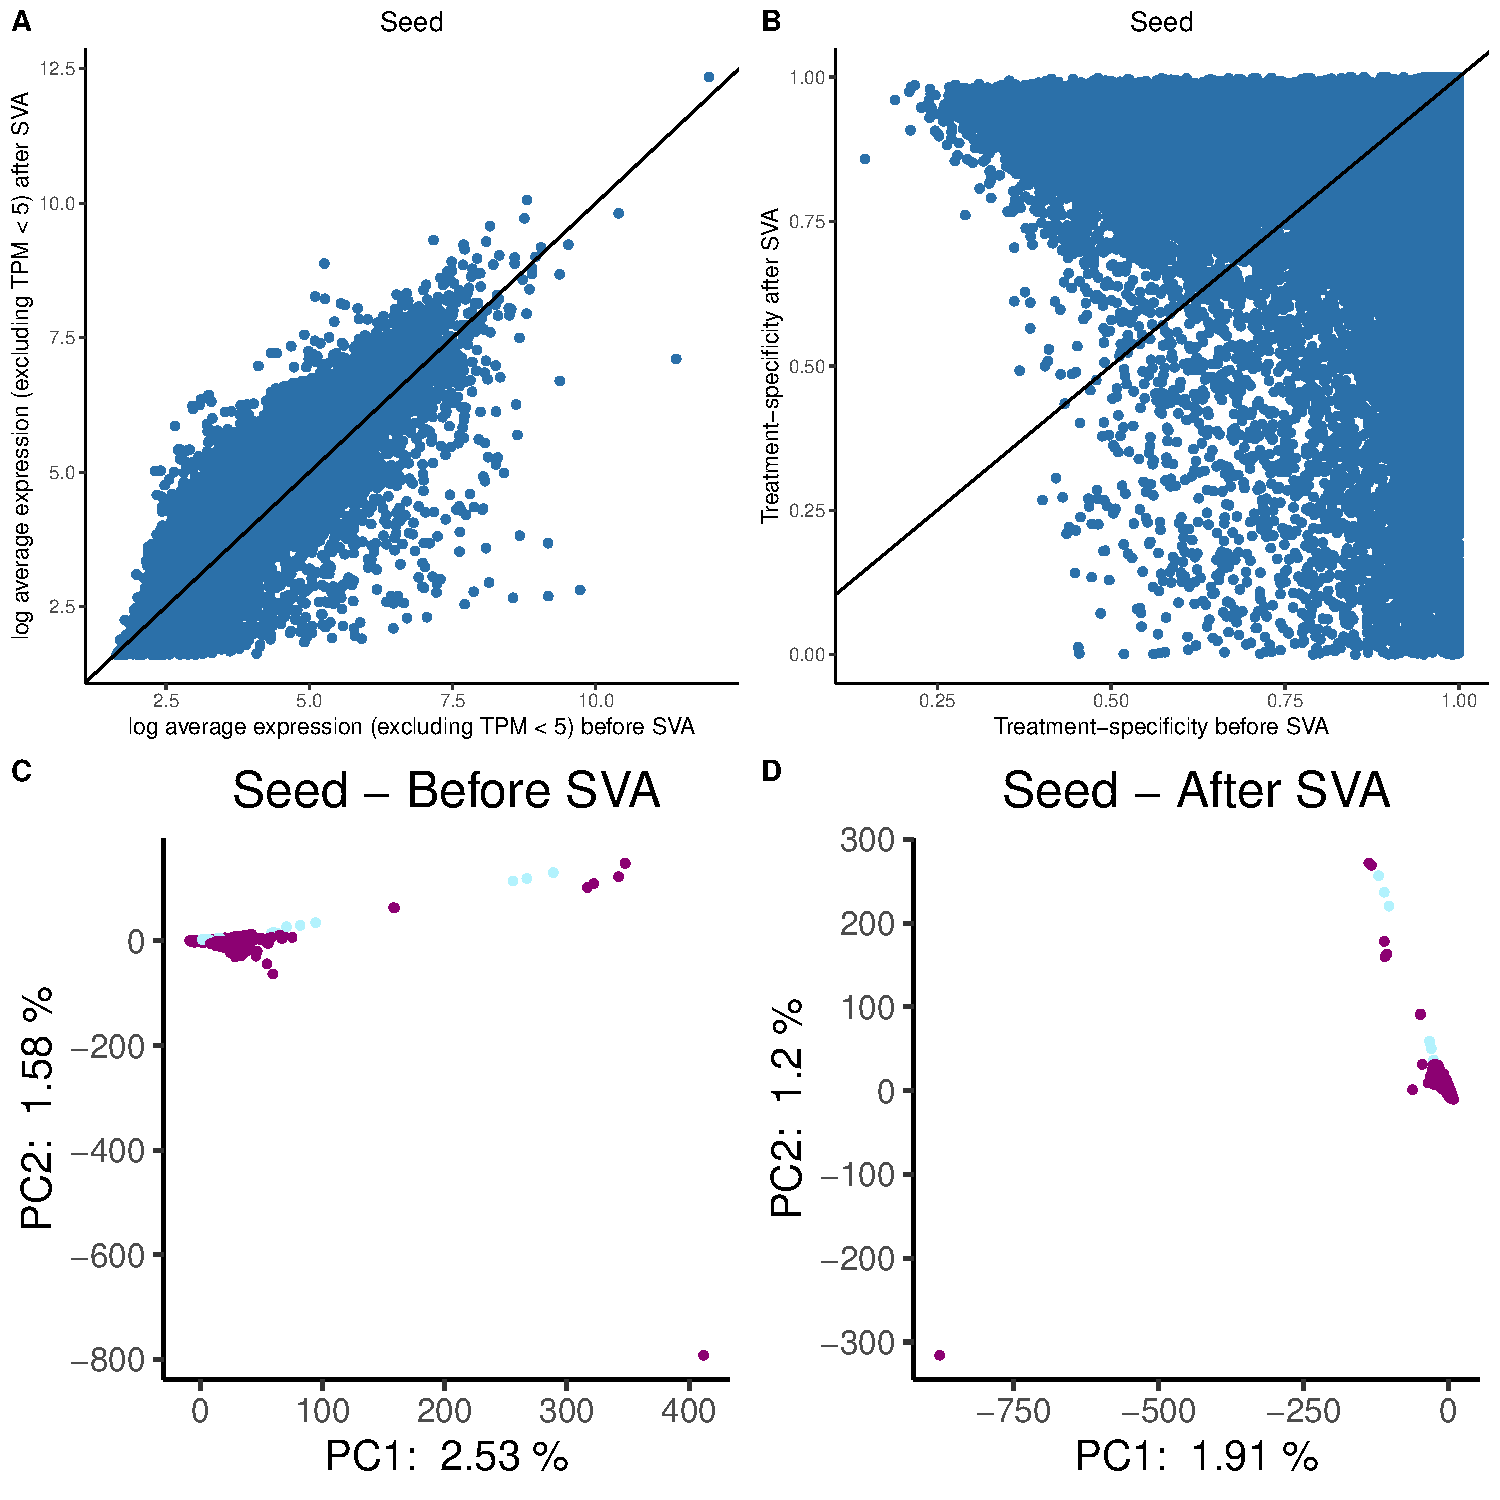
\includegraphics[width = \linewidth]{figures/appendix_a/pca_beforeAndAfterSva_seed_2023-02-21.pdf}
\caption{\textbf{Effect of surrogate variable analysis on structure of seed tissue data.} (\textbf{A}) Effect of SVA on average expression. (\textbf{B}) Effect of SVA on treatment-specificity. (\textbf{C}) Principal component analysis of seed tissue data before SVA. (\textbf{D}) Principal component analysis of seed tissue data after SVA. Color in the PCA plots represent different experimental treatments - legend is Figure \ref{fig::pcaLegendSeed}.}%
\end{figure}

\begin{figure}[H]
\centering
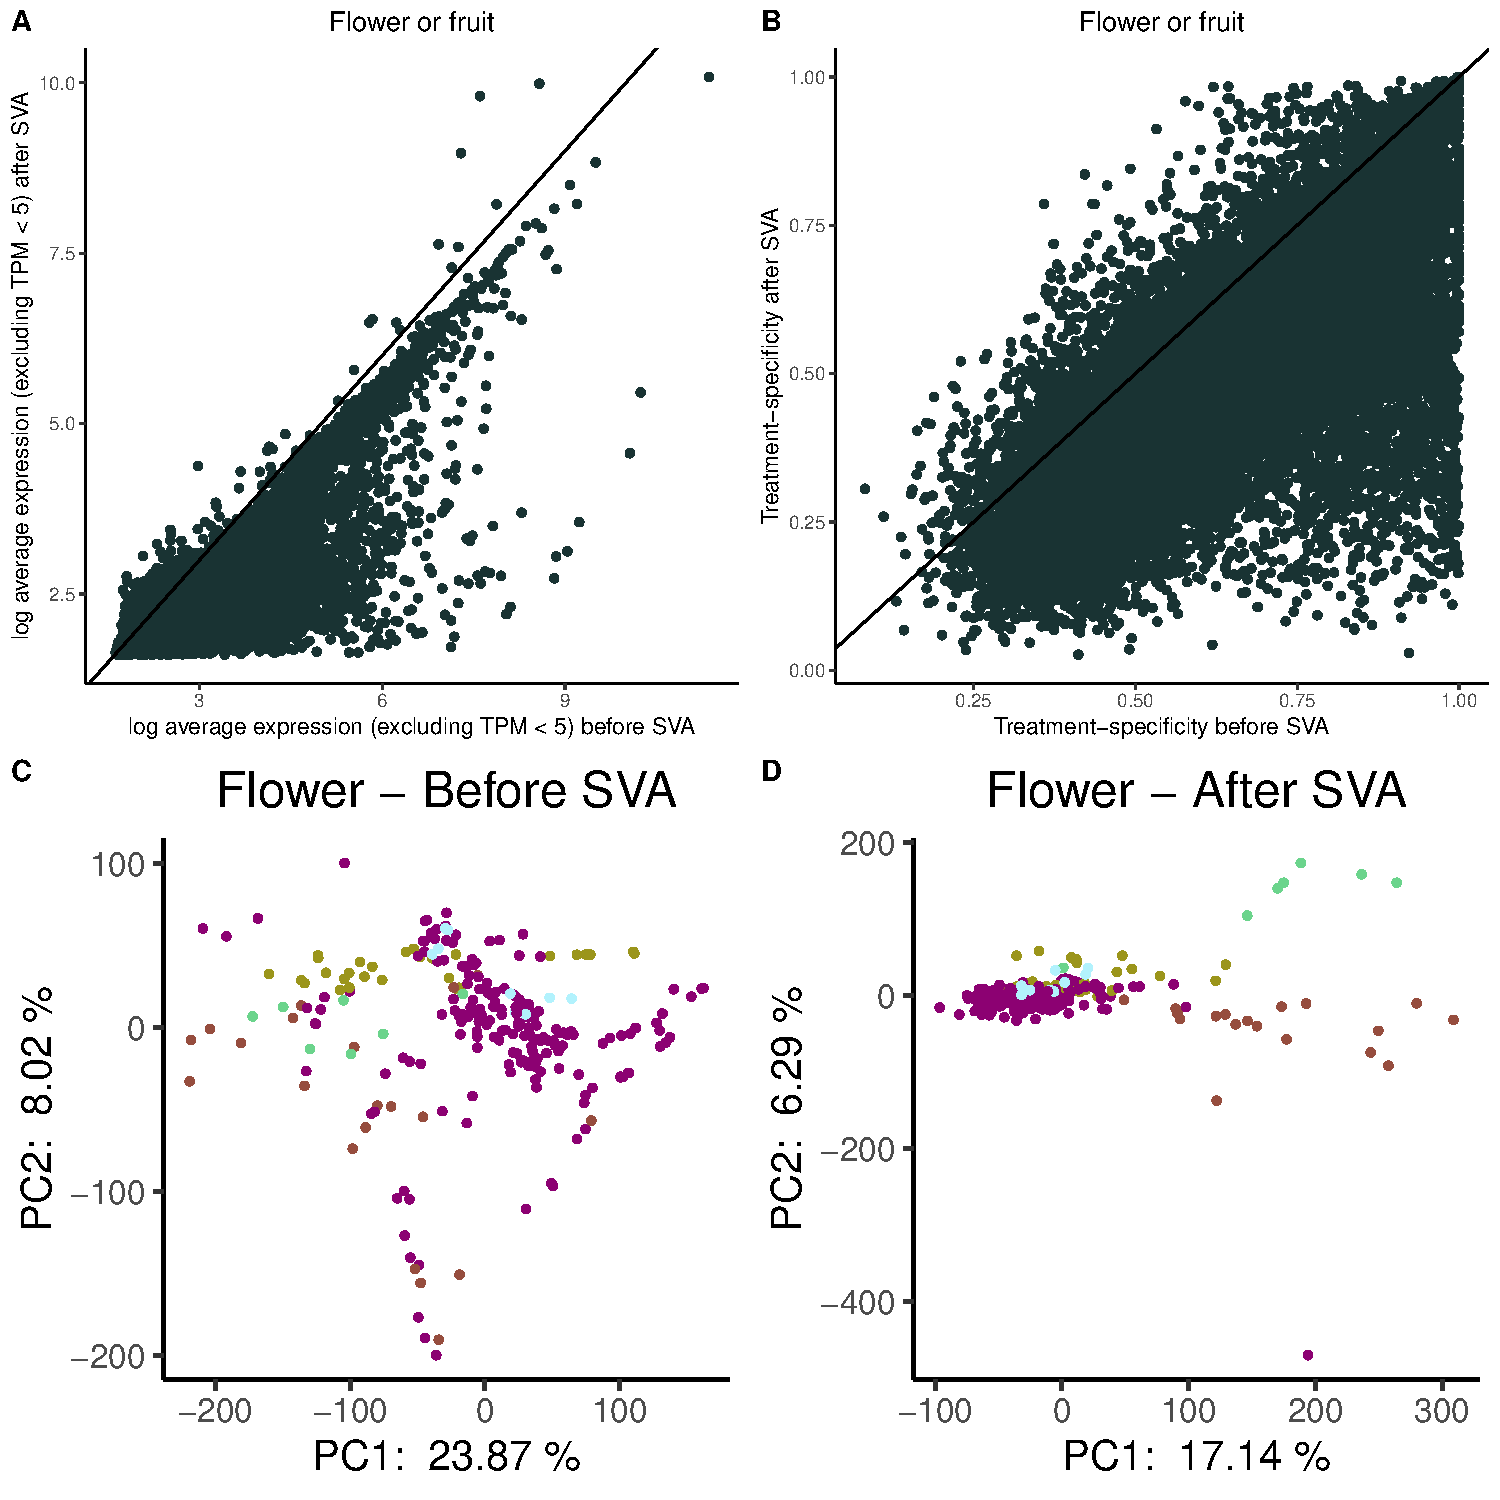
\includegraphics[width = \linewidth]{figures/appendix_a/pca_beforeAndAfterSva_flower_2023-02-21.pdf}
\caption{\textbf{Effect of surrogate variable analysis on structure of fruit and flower tissue data.} (\textbf{A}) Effect of SVA on average expression. (\textbf{B}) Effect of SVA on treatment-specificity. (\textbf{C}) Principal component analysis of fruit and flower tissue data before SVA. (\textbf{D}) Principal component analysis of fruit and flower tissue data after SVA. Color in the PCA plots represent different experimental treatments - legend is Figure \ref{fig::pcaLegendFlower}.}%
\end{figure}

\subsection*{Legends - PCA before and after SVA on data subset by tissue type}

\begin{figure}[H]
\centering
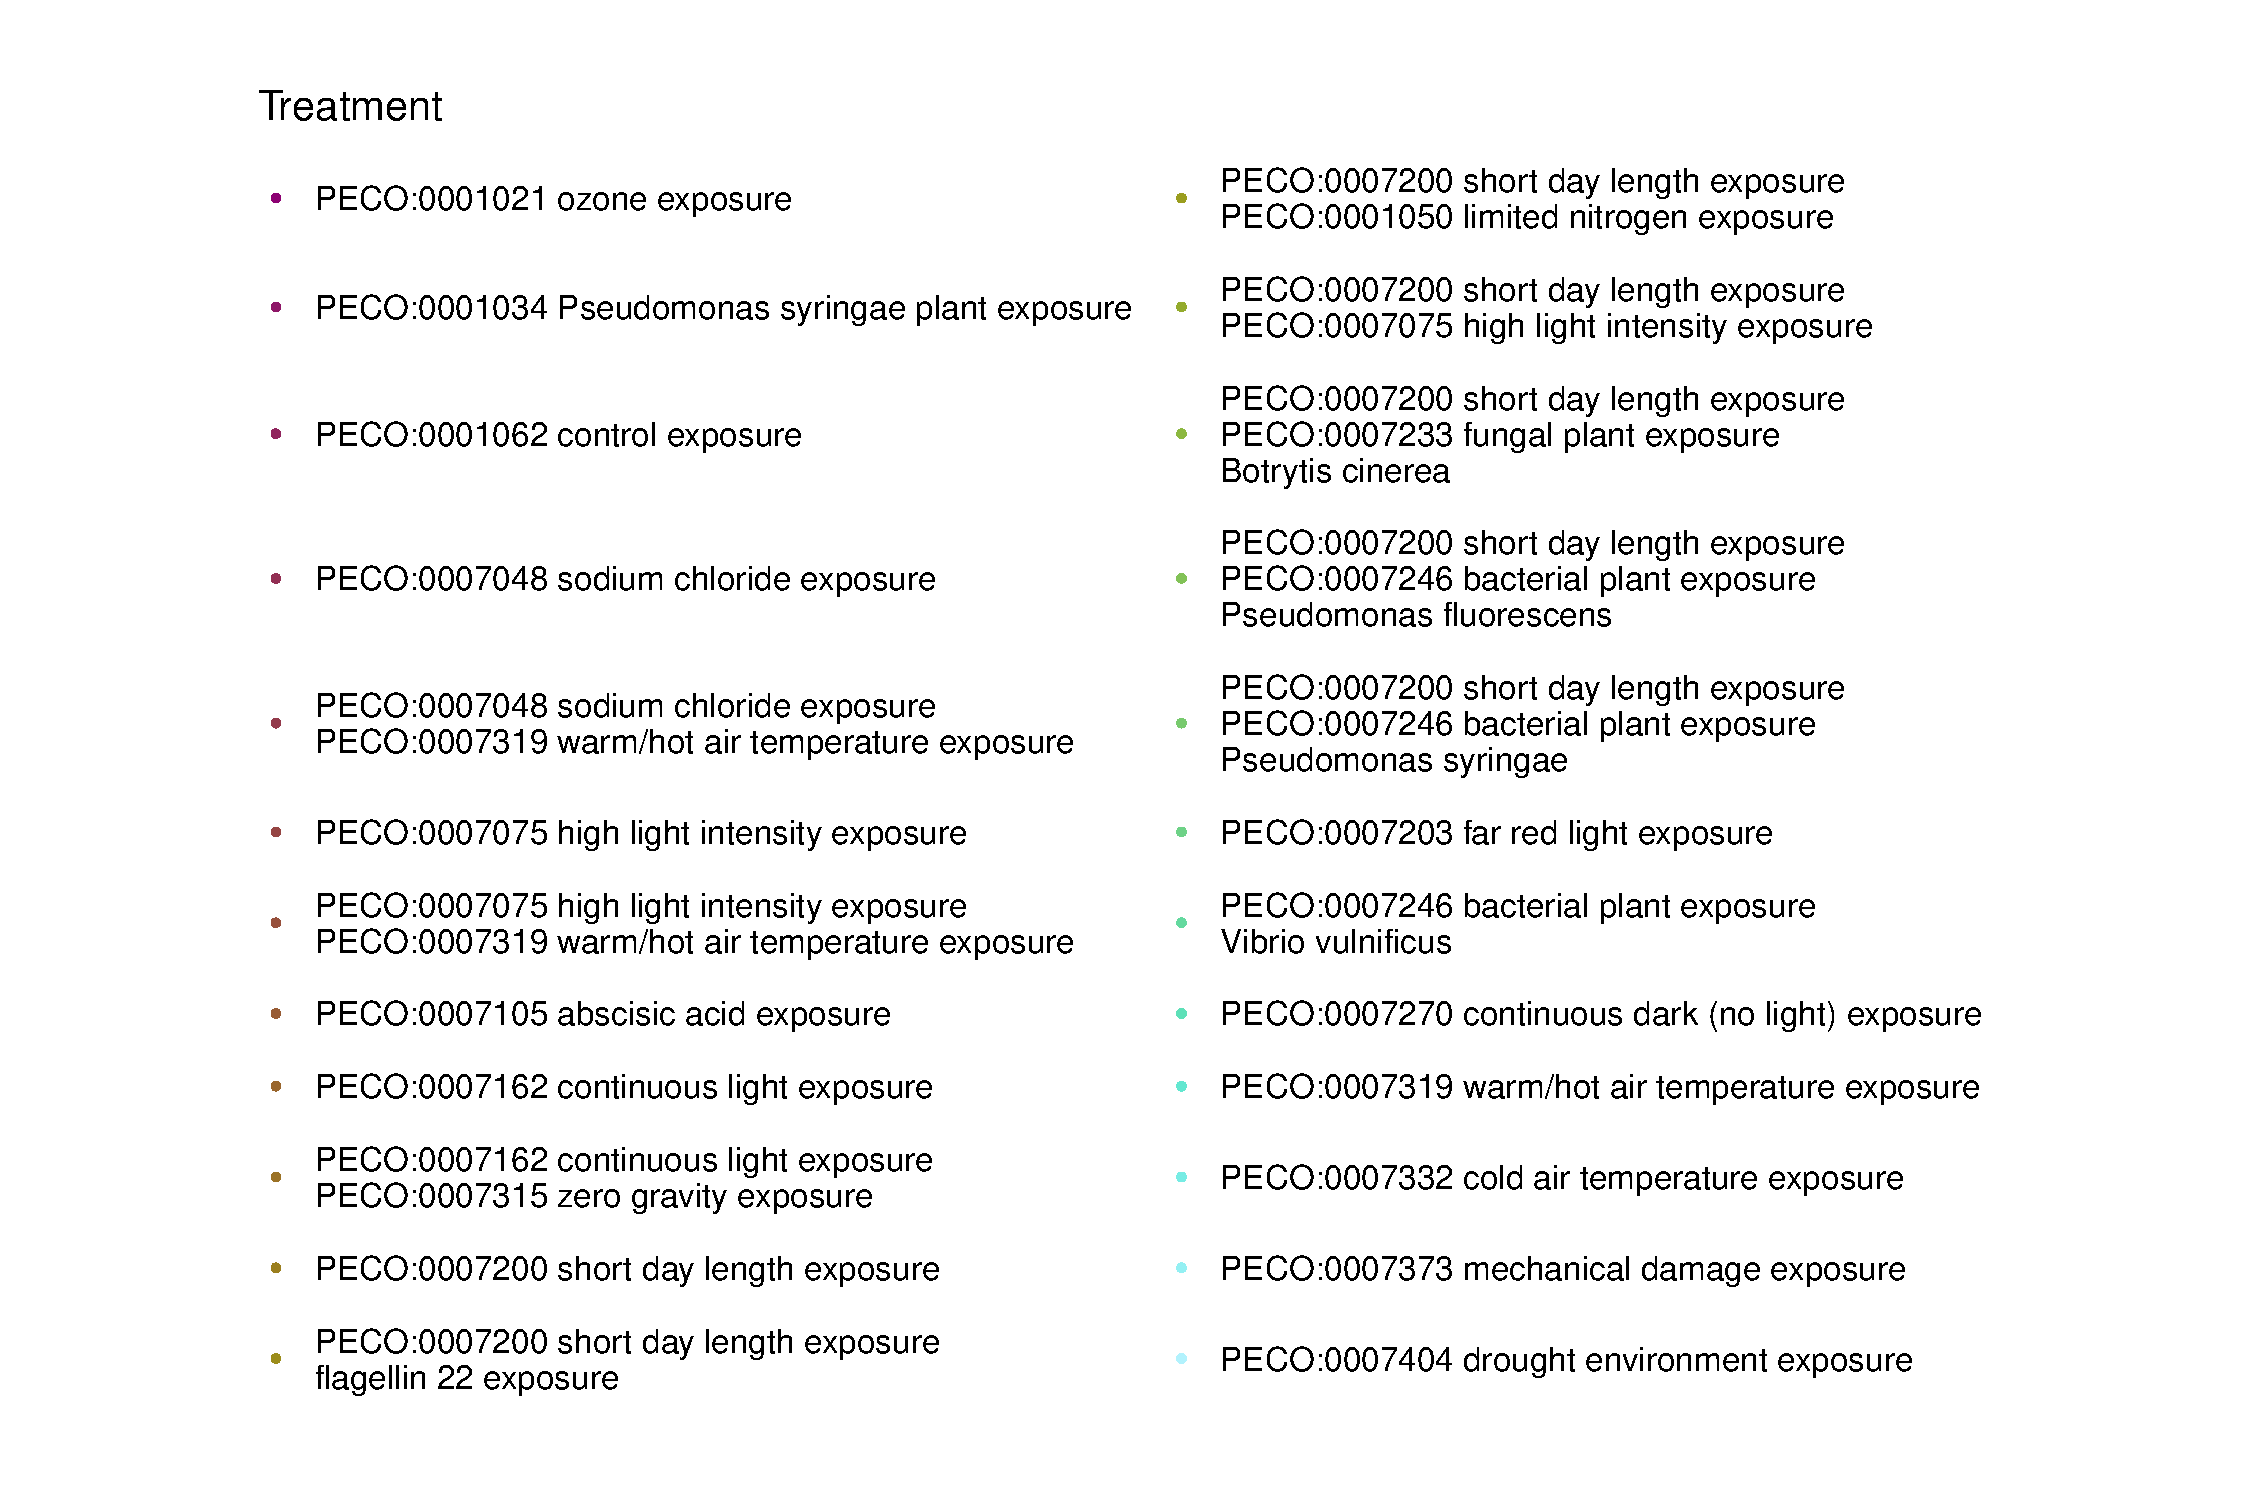
\includegraphics[width = \linewidth]{figures/appendix_a/pca_beforeAndAfterSva_leaf_legend_2023-02-21.pdf}
\caption{\textbf{Legend for PCA before and after SVA, leaf data.}}%
\label{fig::pcaLegendLeaf}
\end{figure}

\begin{figure}[H]
\centering
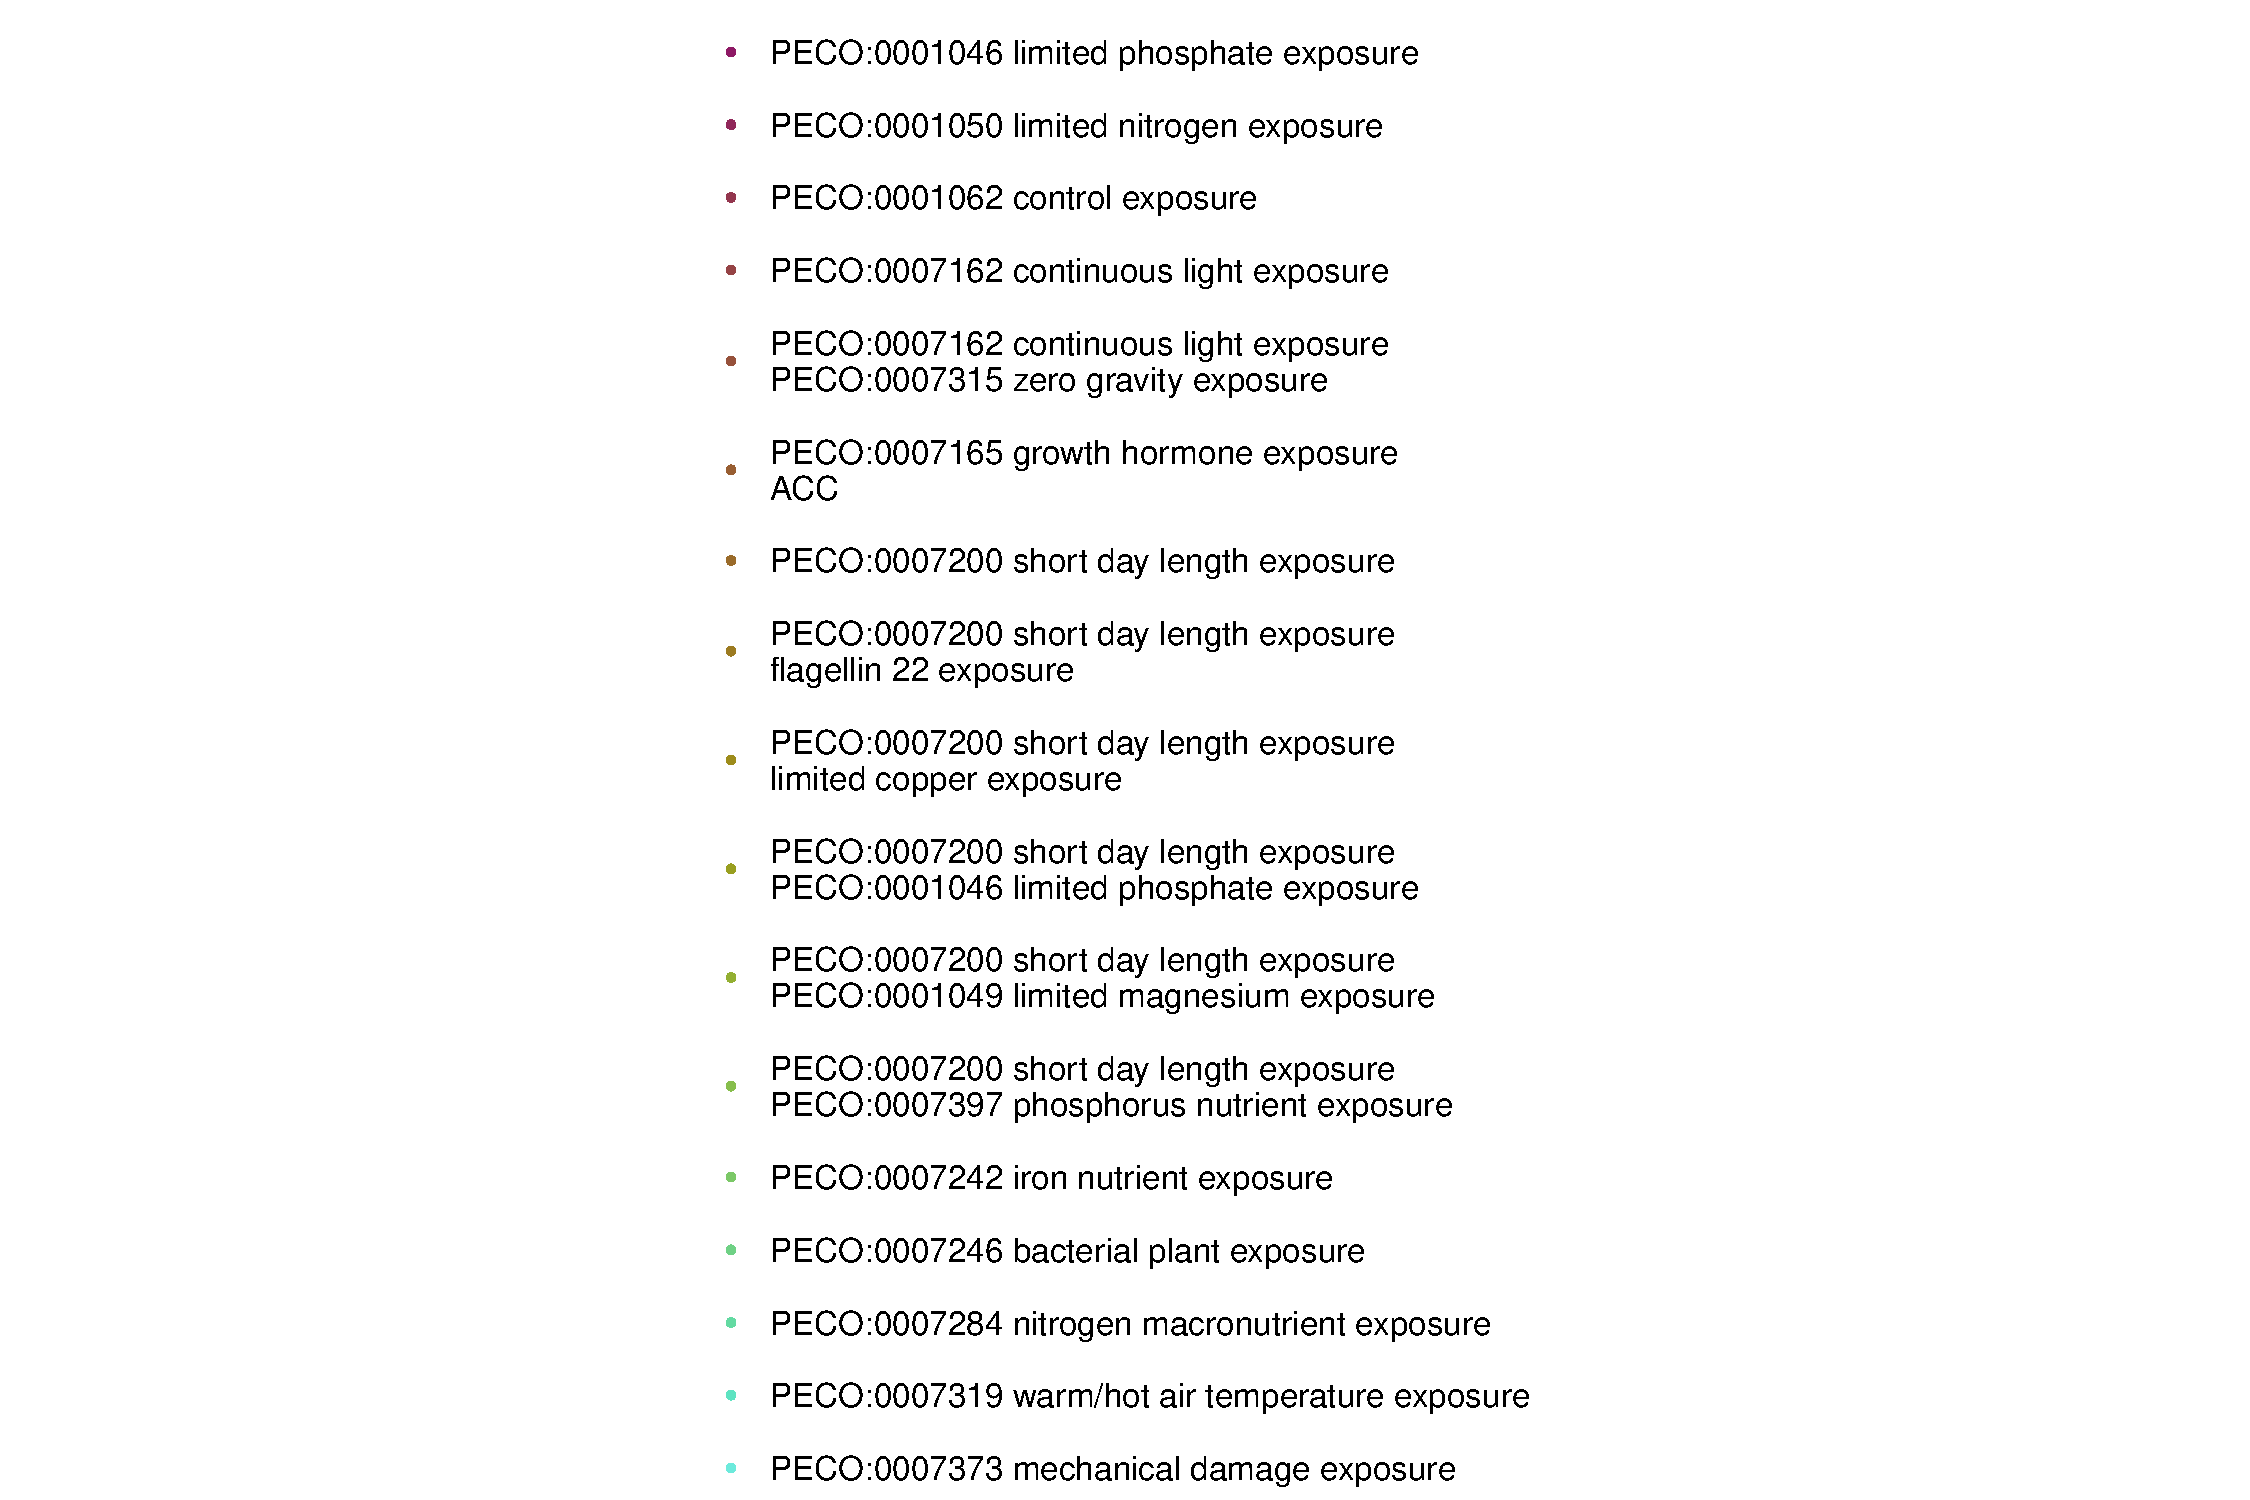
\includegraphics[width = \linewidth]{figures/appendix_a/pca_beforeAndAfterSva_root_legend_2023-02-21.pdf}
\caption{\textbf{Legend for PCA before and after SVA, root data.}}%
\label{fig::pcaLegendRoot}
\end{figure}

\begin{figure}[H]
\centering
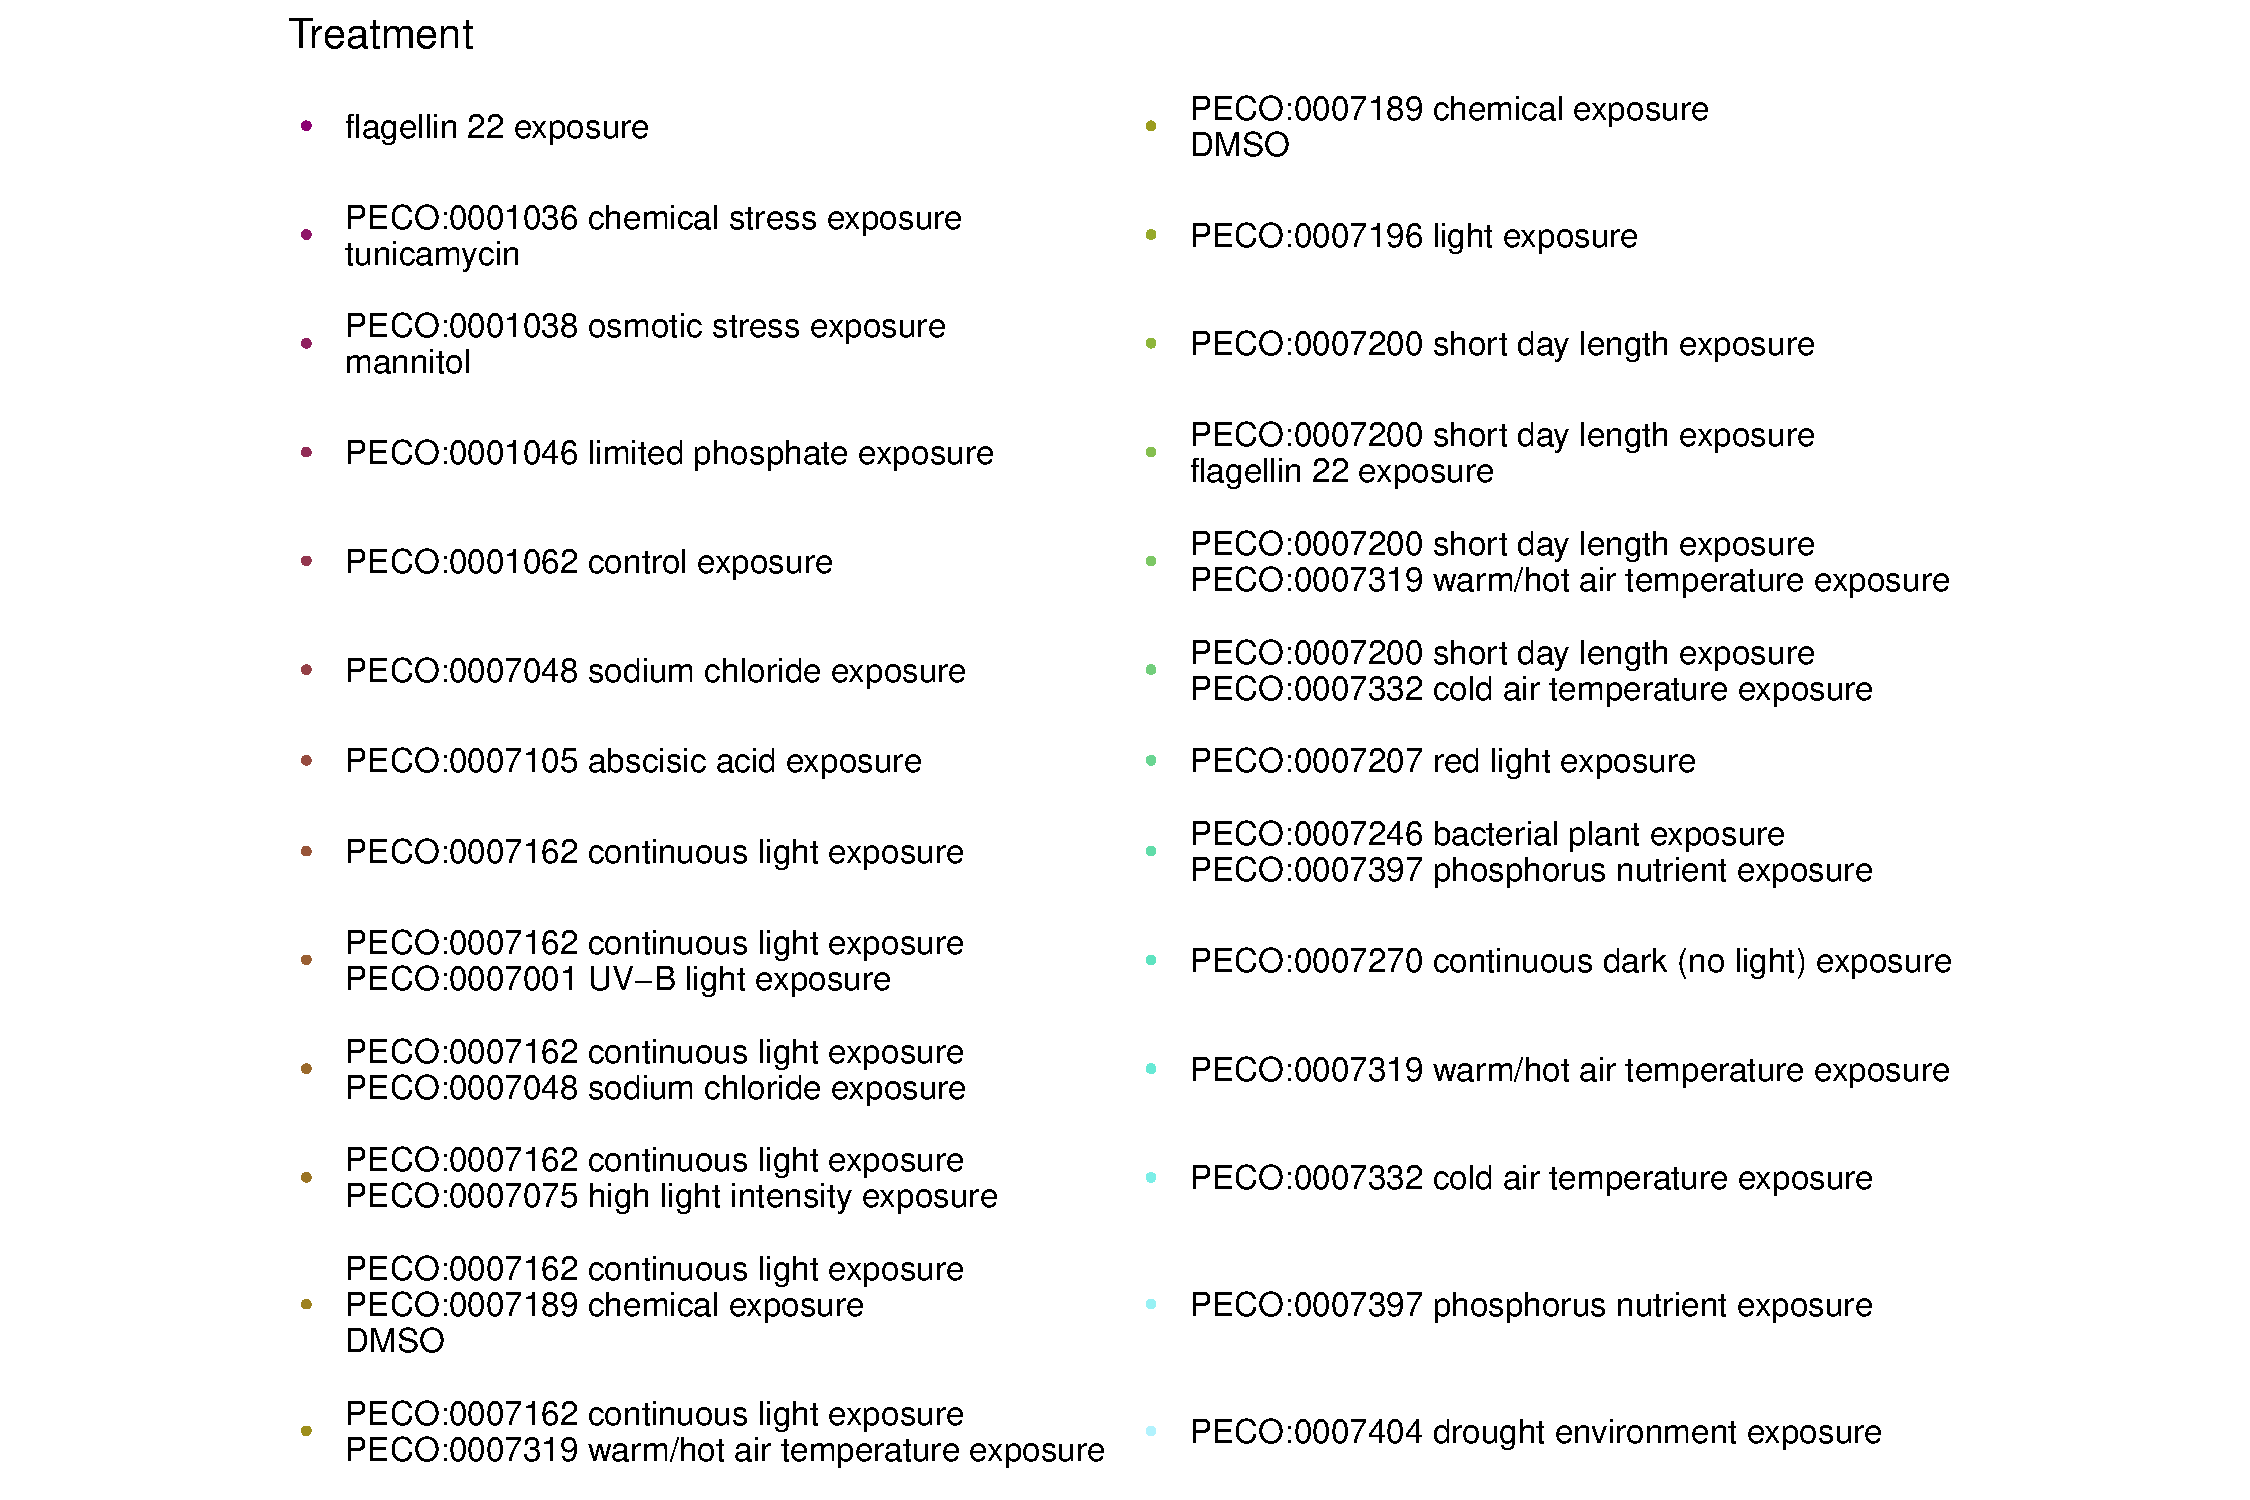
\includegraphics[width = \linewidth]{figures/appendix_a/pca_beforeAndAfterSva_plant_legend_2023-02-21.pdf}
\caption{\textbf{Legend for PCA before and after SVA, whole plant data.}}%
\label{fig::pcaLegendPlant}
\end{figure}

\begin{figure}[H]
\centering
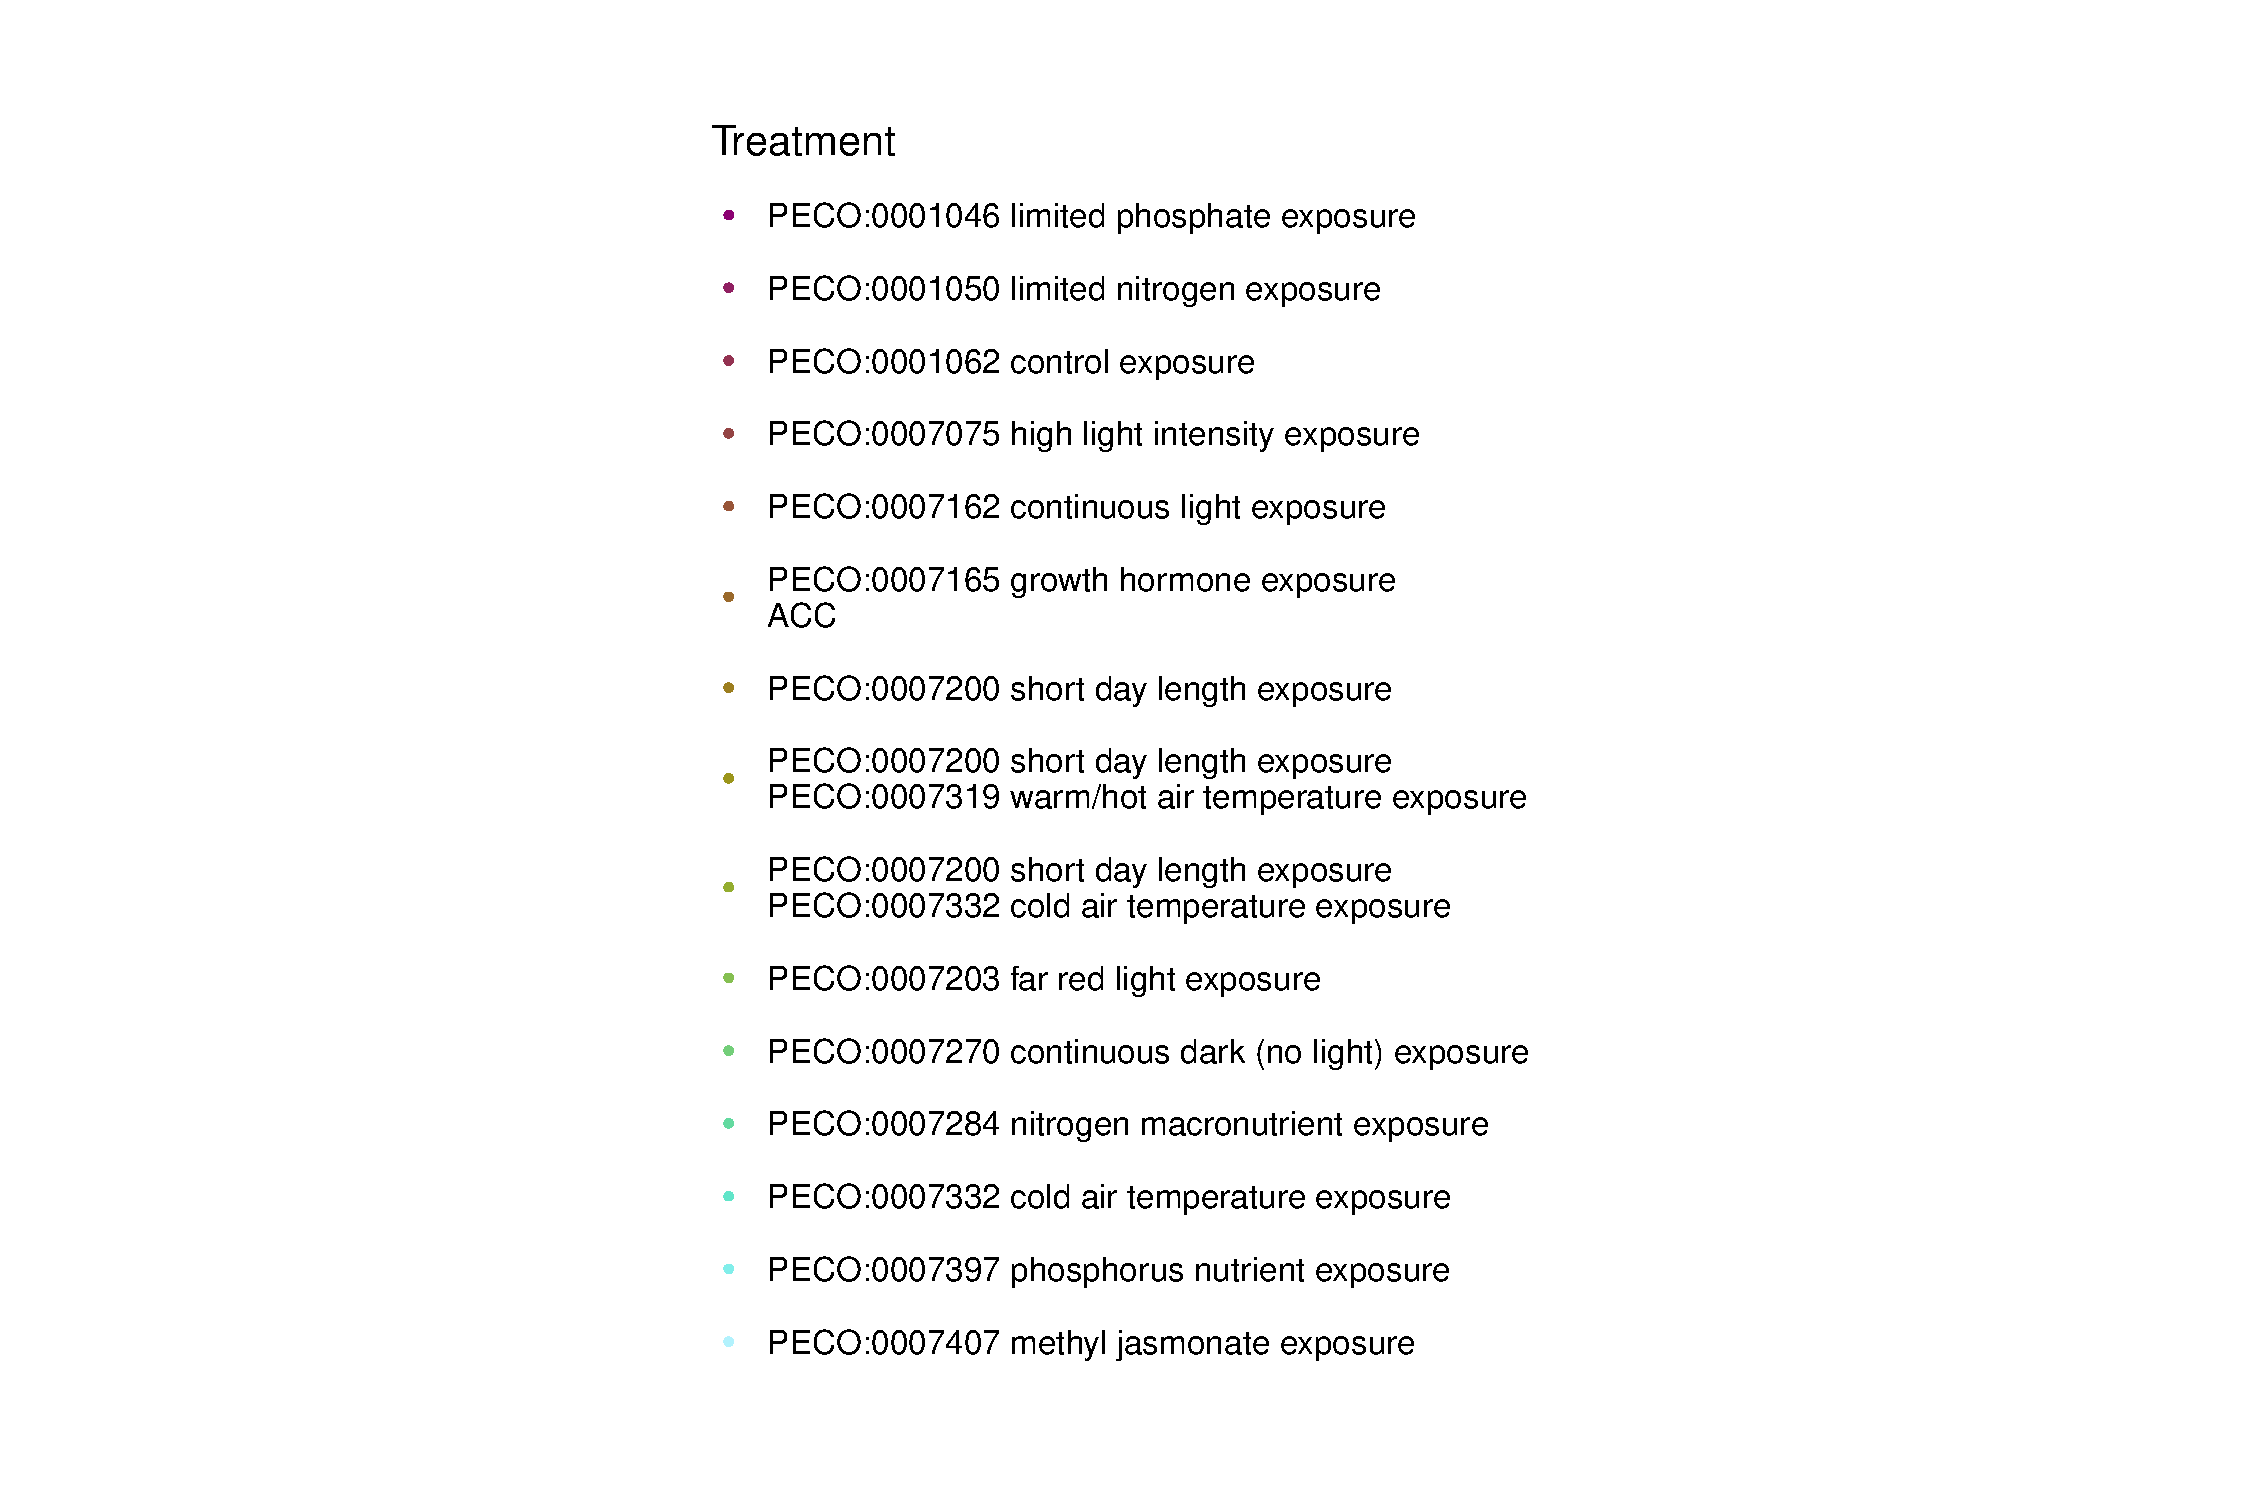
\includegraphics[width = \linewidth]{figures/appendix_a/pca_beforeAndAfterSva_shoot_legend_2023-02-21.pdf}
\caption{\textbf{Legend for PCA before and after SVA, shoot data.}}%
\label{fig::pcaLegendShoot}
\end{figure}

\begin{figure}[H]
\centering
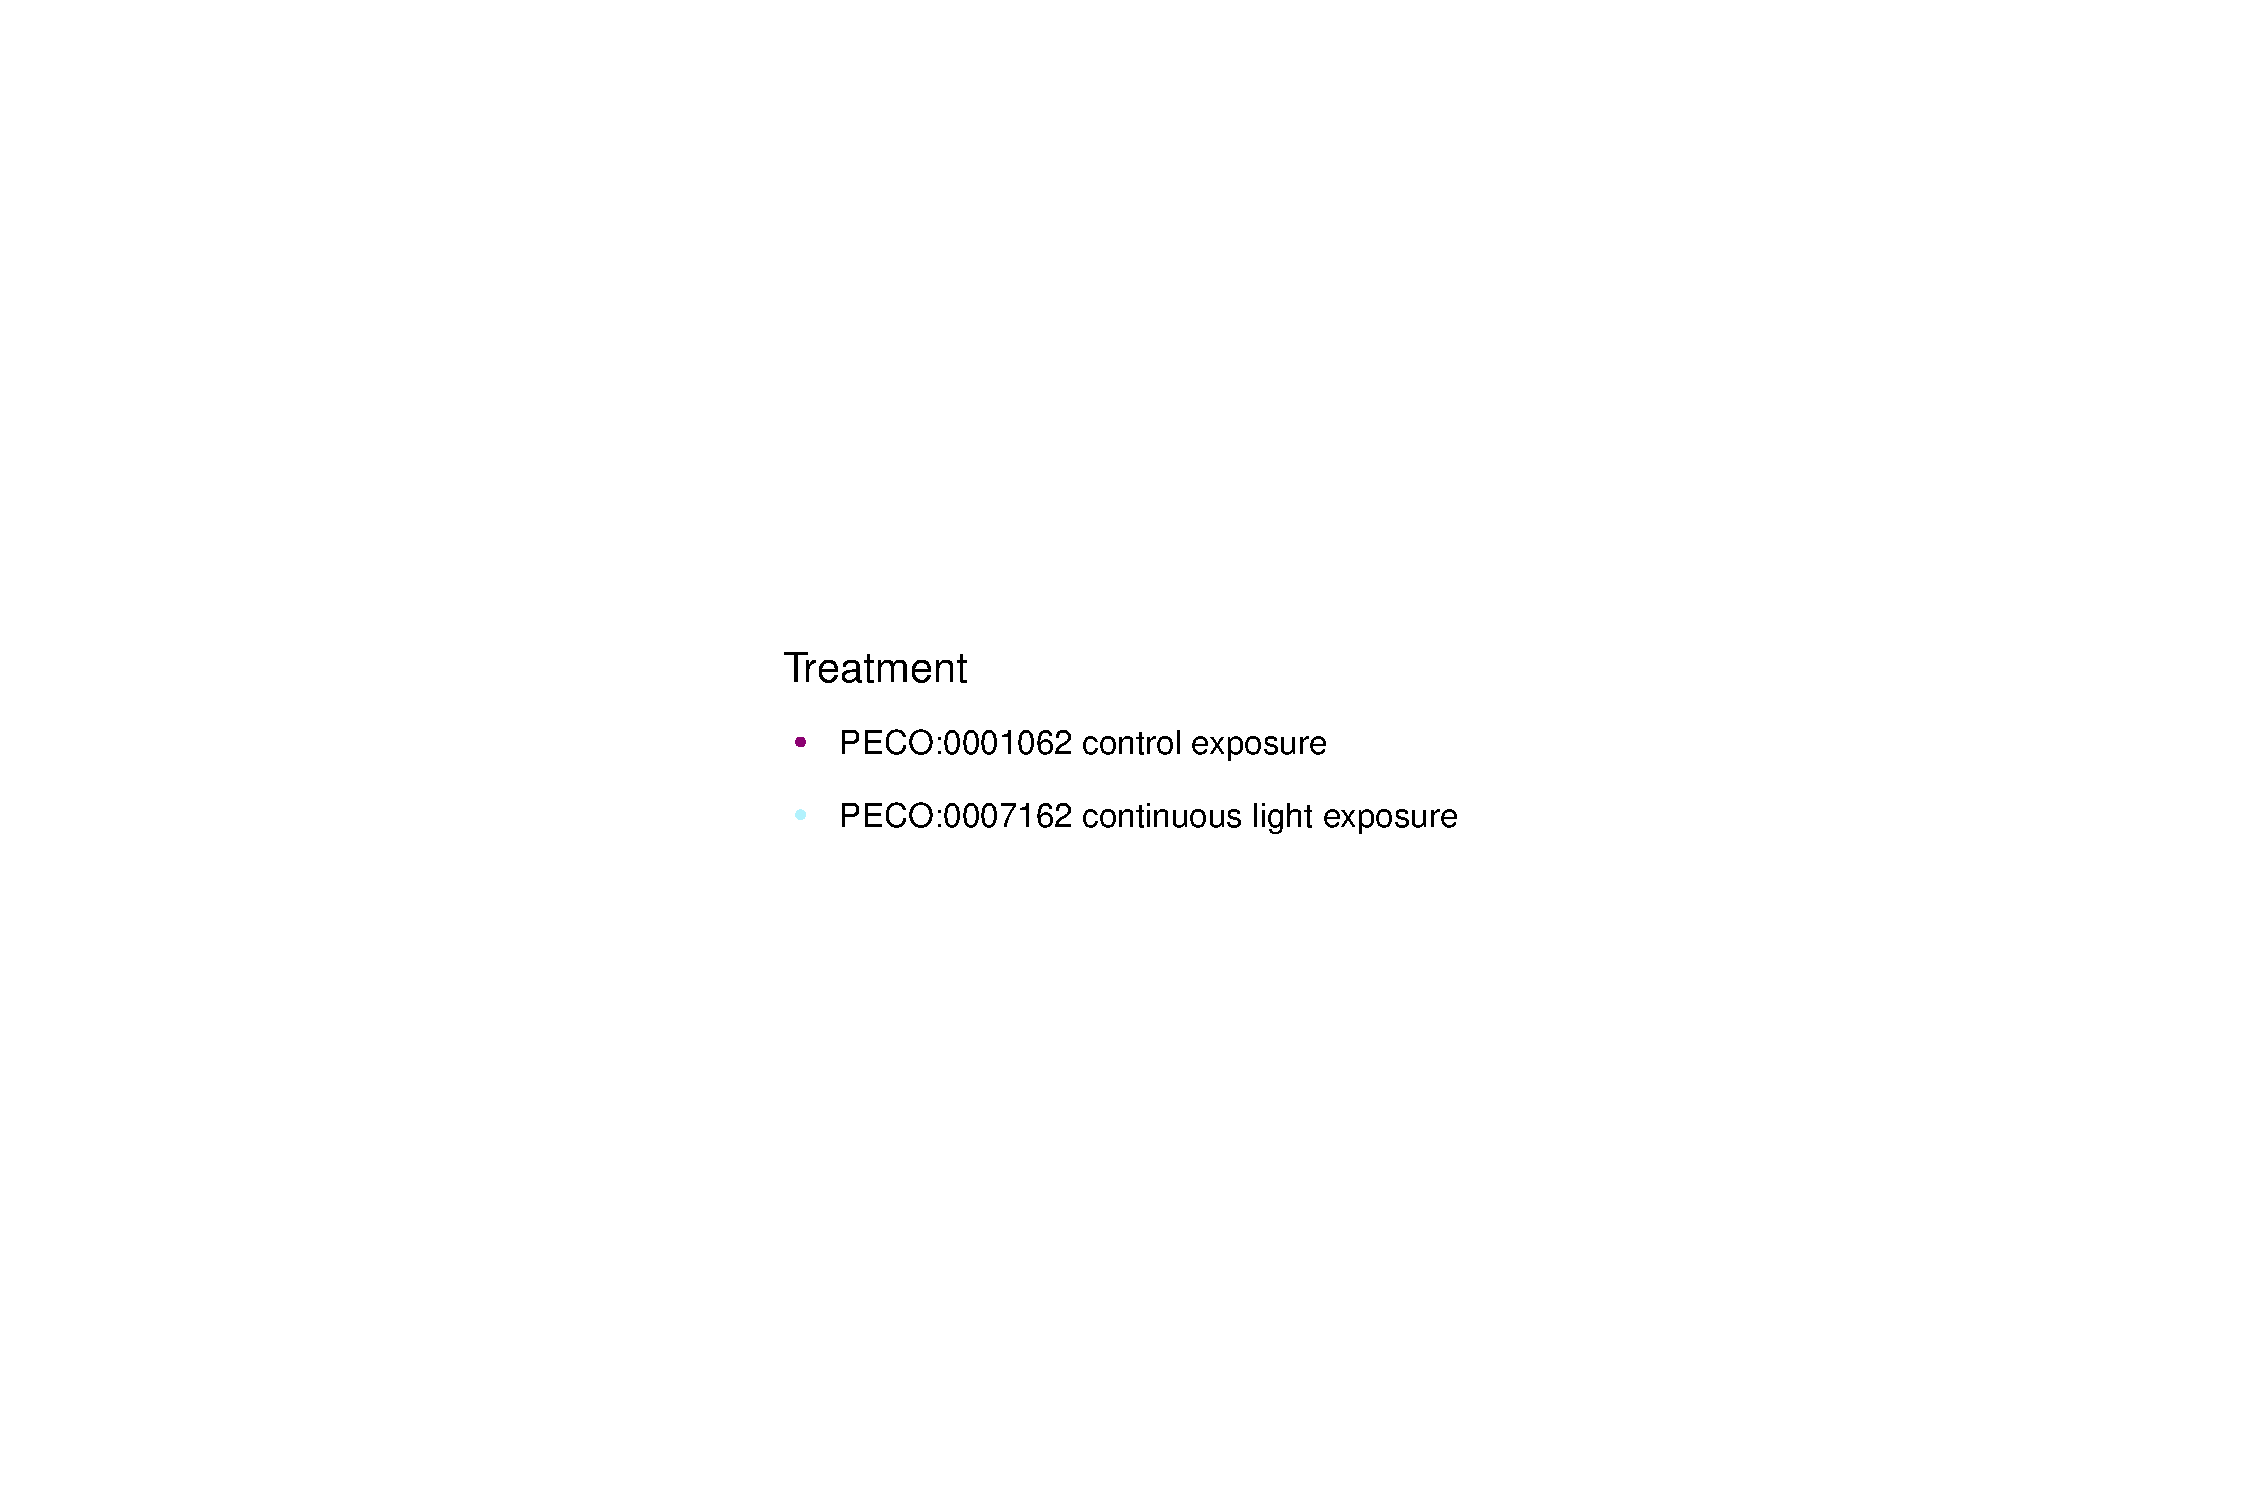
\includegraphics[width = \linewidth]{figures/appendix_a/pca_beforeAndAfterSva_seed_legend_2023-02-21.pdf}
\caption{\textbf{Legend for PCA before and after SVA, seed data.}}%
\label{fig::pcaLegendSeed}
\end{figure}

\begin{figure}[H]
\centering
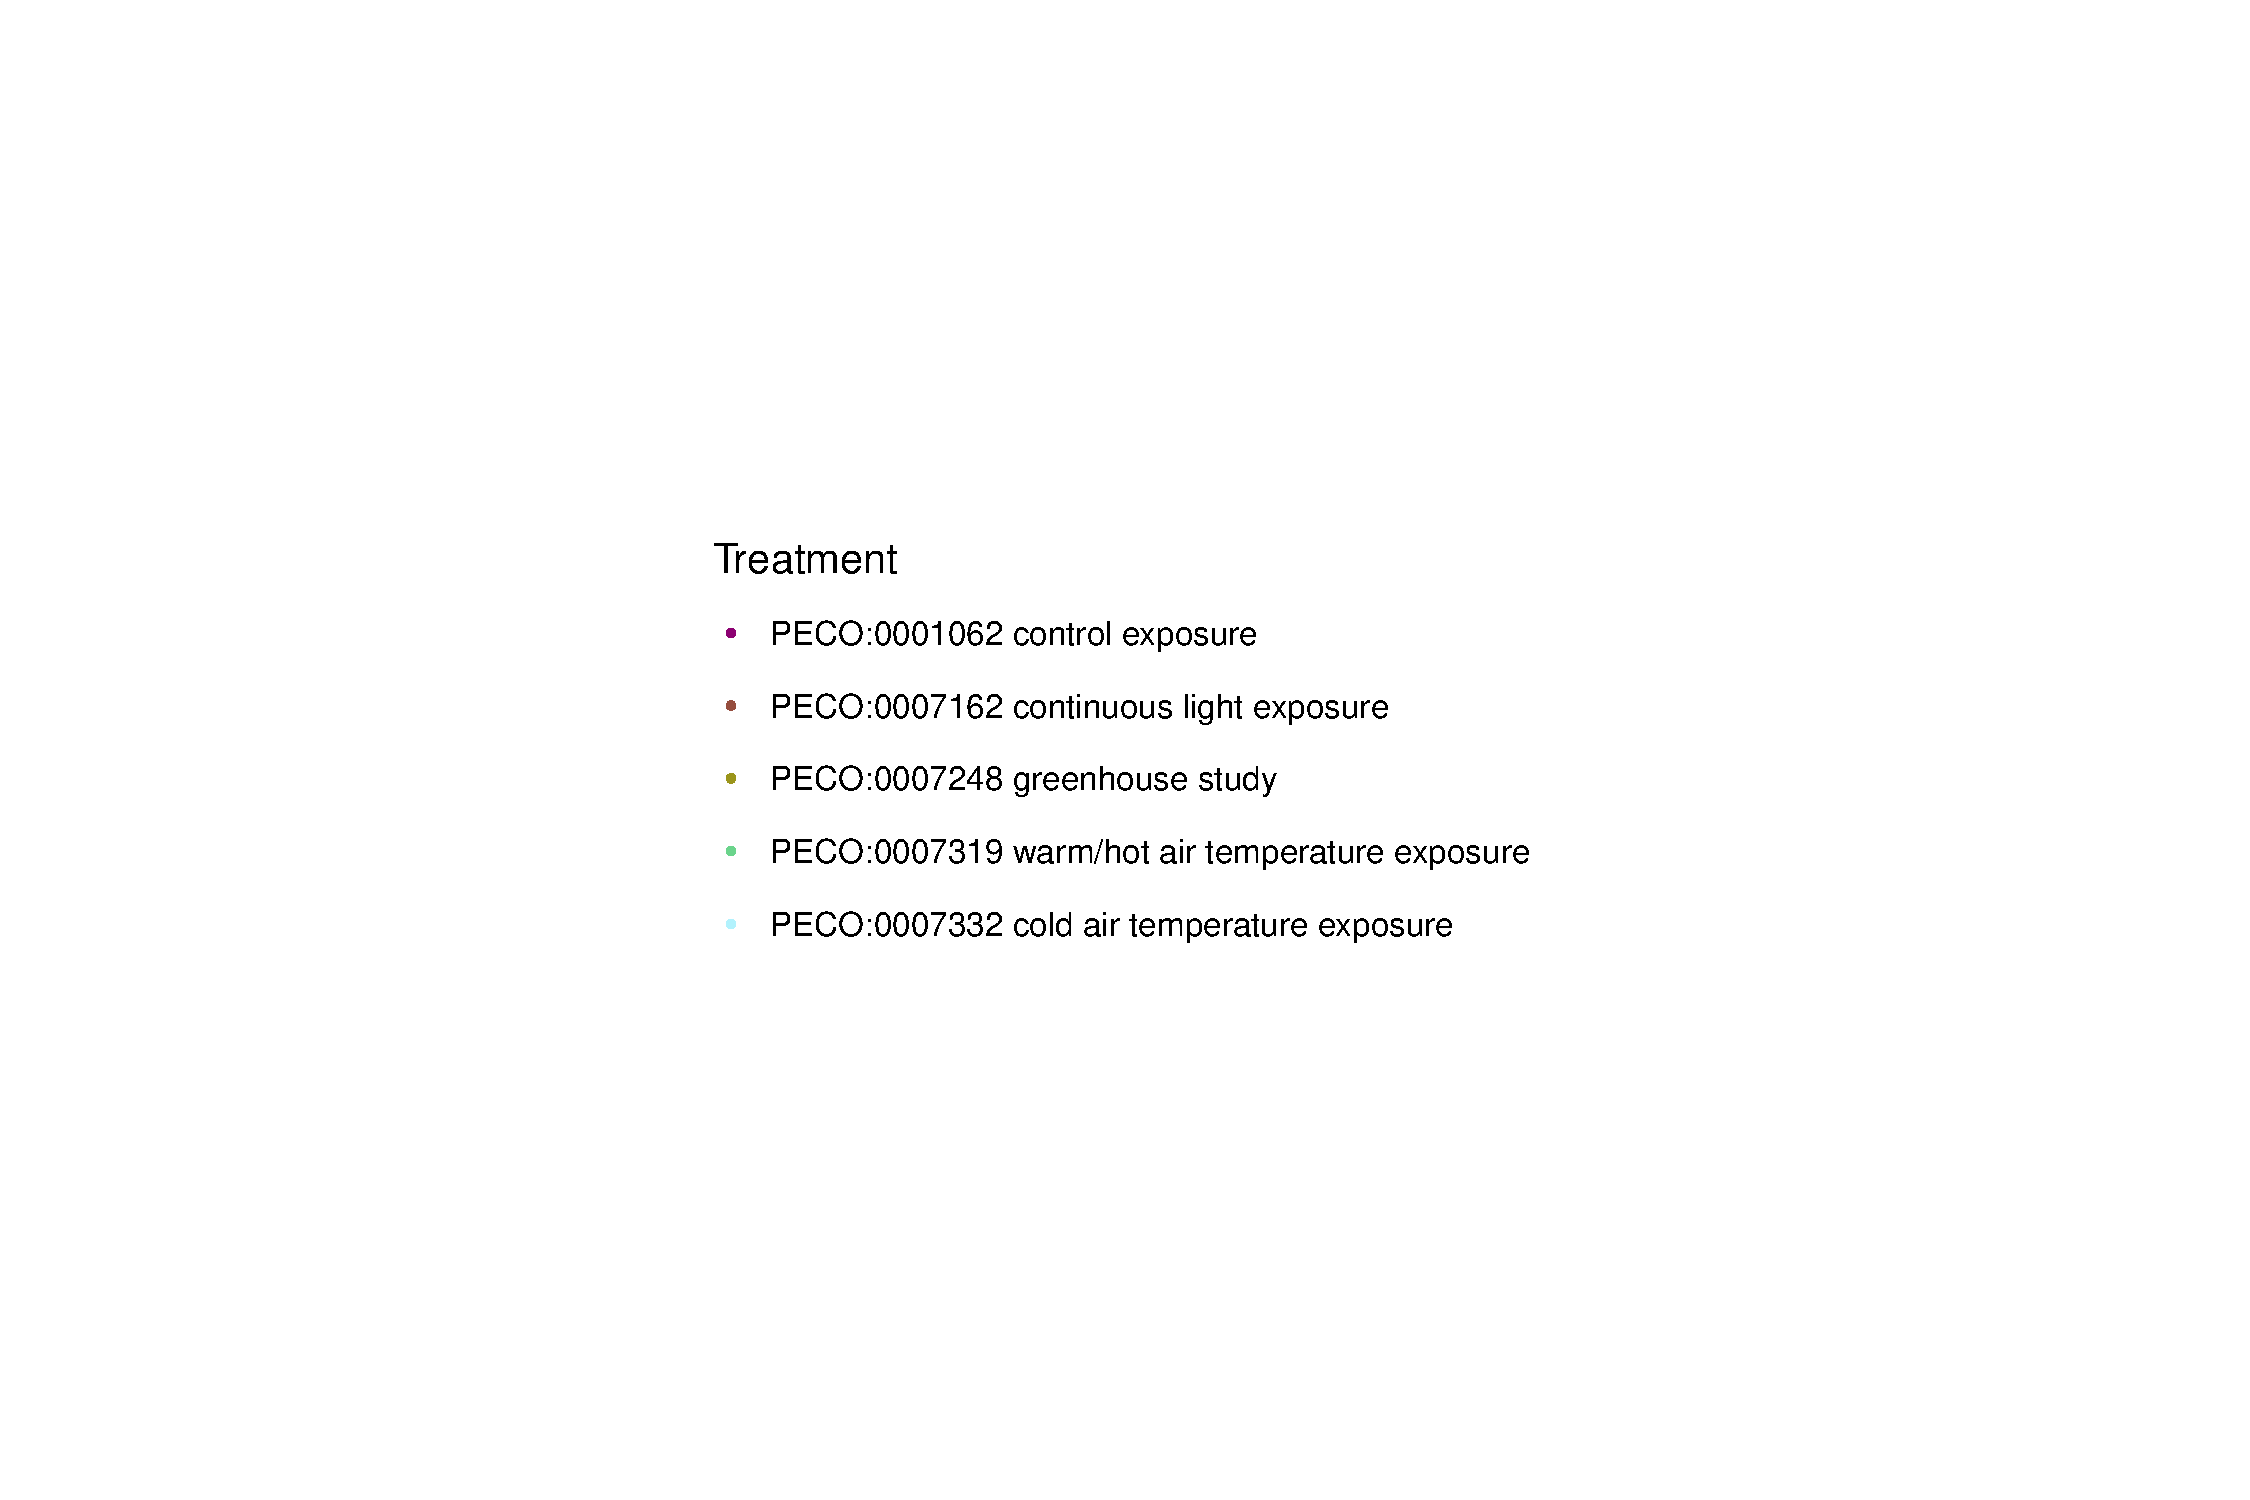
\includegraphics[width = \linewidth]{figures/appendix_a/pca_beforeAndAfterSva_flower_legend_2023-02-21.pdf}
\caption{\textbf{Legend for PCA before and after SVA, flower data.}}%
\label{fig::pcaLegendFlower}
\end{figure}

\newpage % force section header onto next page with figure
\subsection*{Partial correlations, balanced subset after SVA}

\begin{figure}[H]
\centering
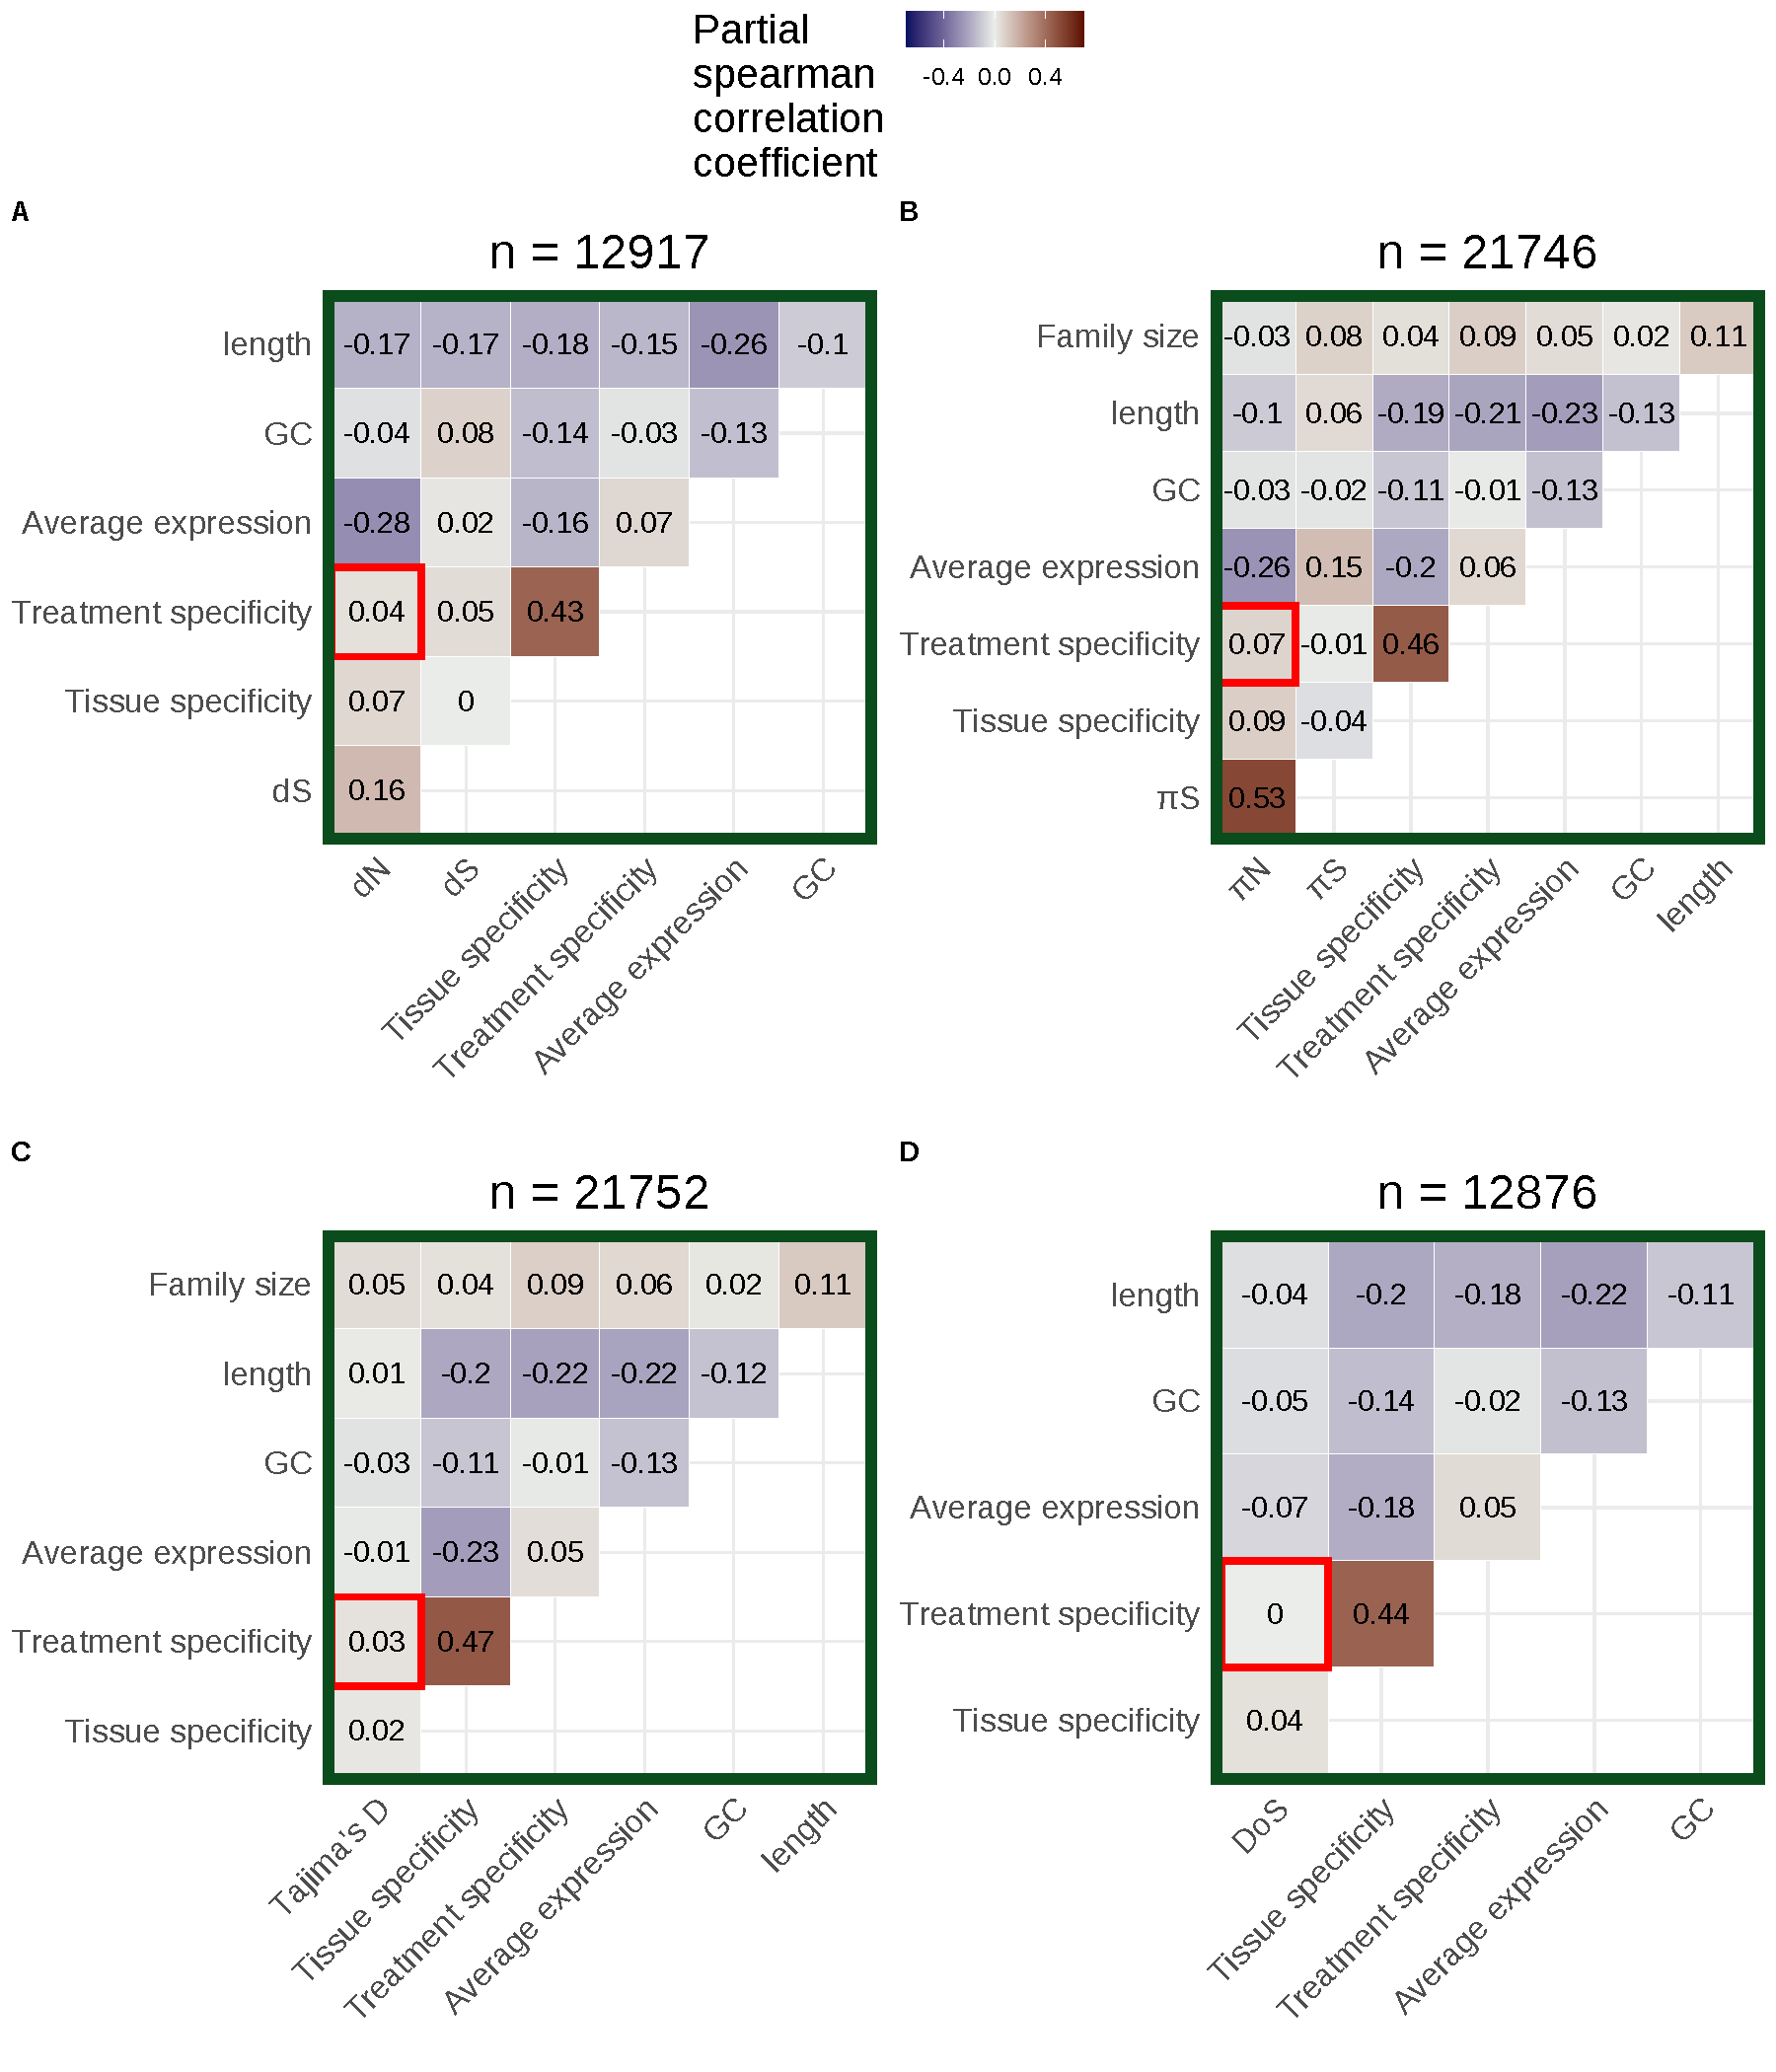
\includegraphics[width = \linewidth]{figures/appendix_a/partialCorrelations_fullyBalancedSubset_leaf_2023-02-22.pdf}
\caption{\textbf{Partial correlation analysis of leaf tissue on balanced data subset after SVA.} Partial correlations for (\textbf{A}) $dN$, (\textbf{B}) $\pi_N$, (\textbf{C}) Tajima's D, and (\textbf{D}) direction of selection (DoS) after applying SVA. Average expression and tissue specificity are calculated using only leaf tissue data. The number of genes included in each partial correlation analysis (n) is listed at the top of each heatmap.}%
\end{figure}

\begin{figure}[H]
\centering
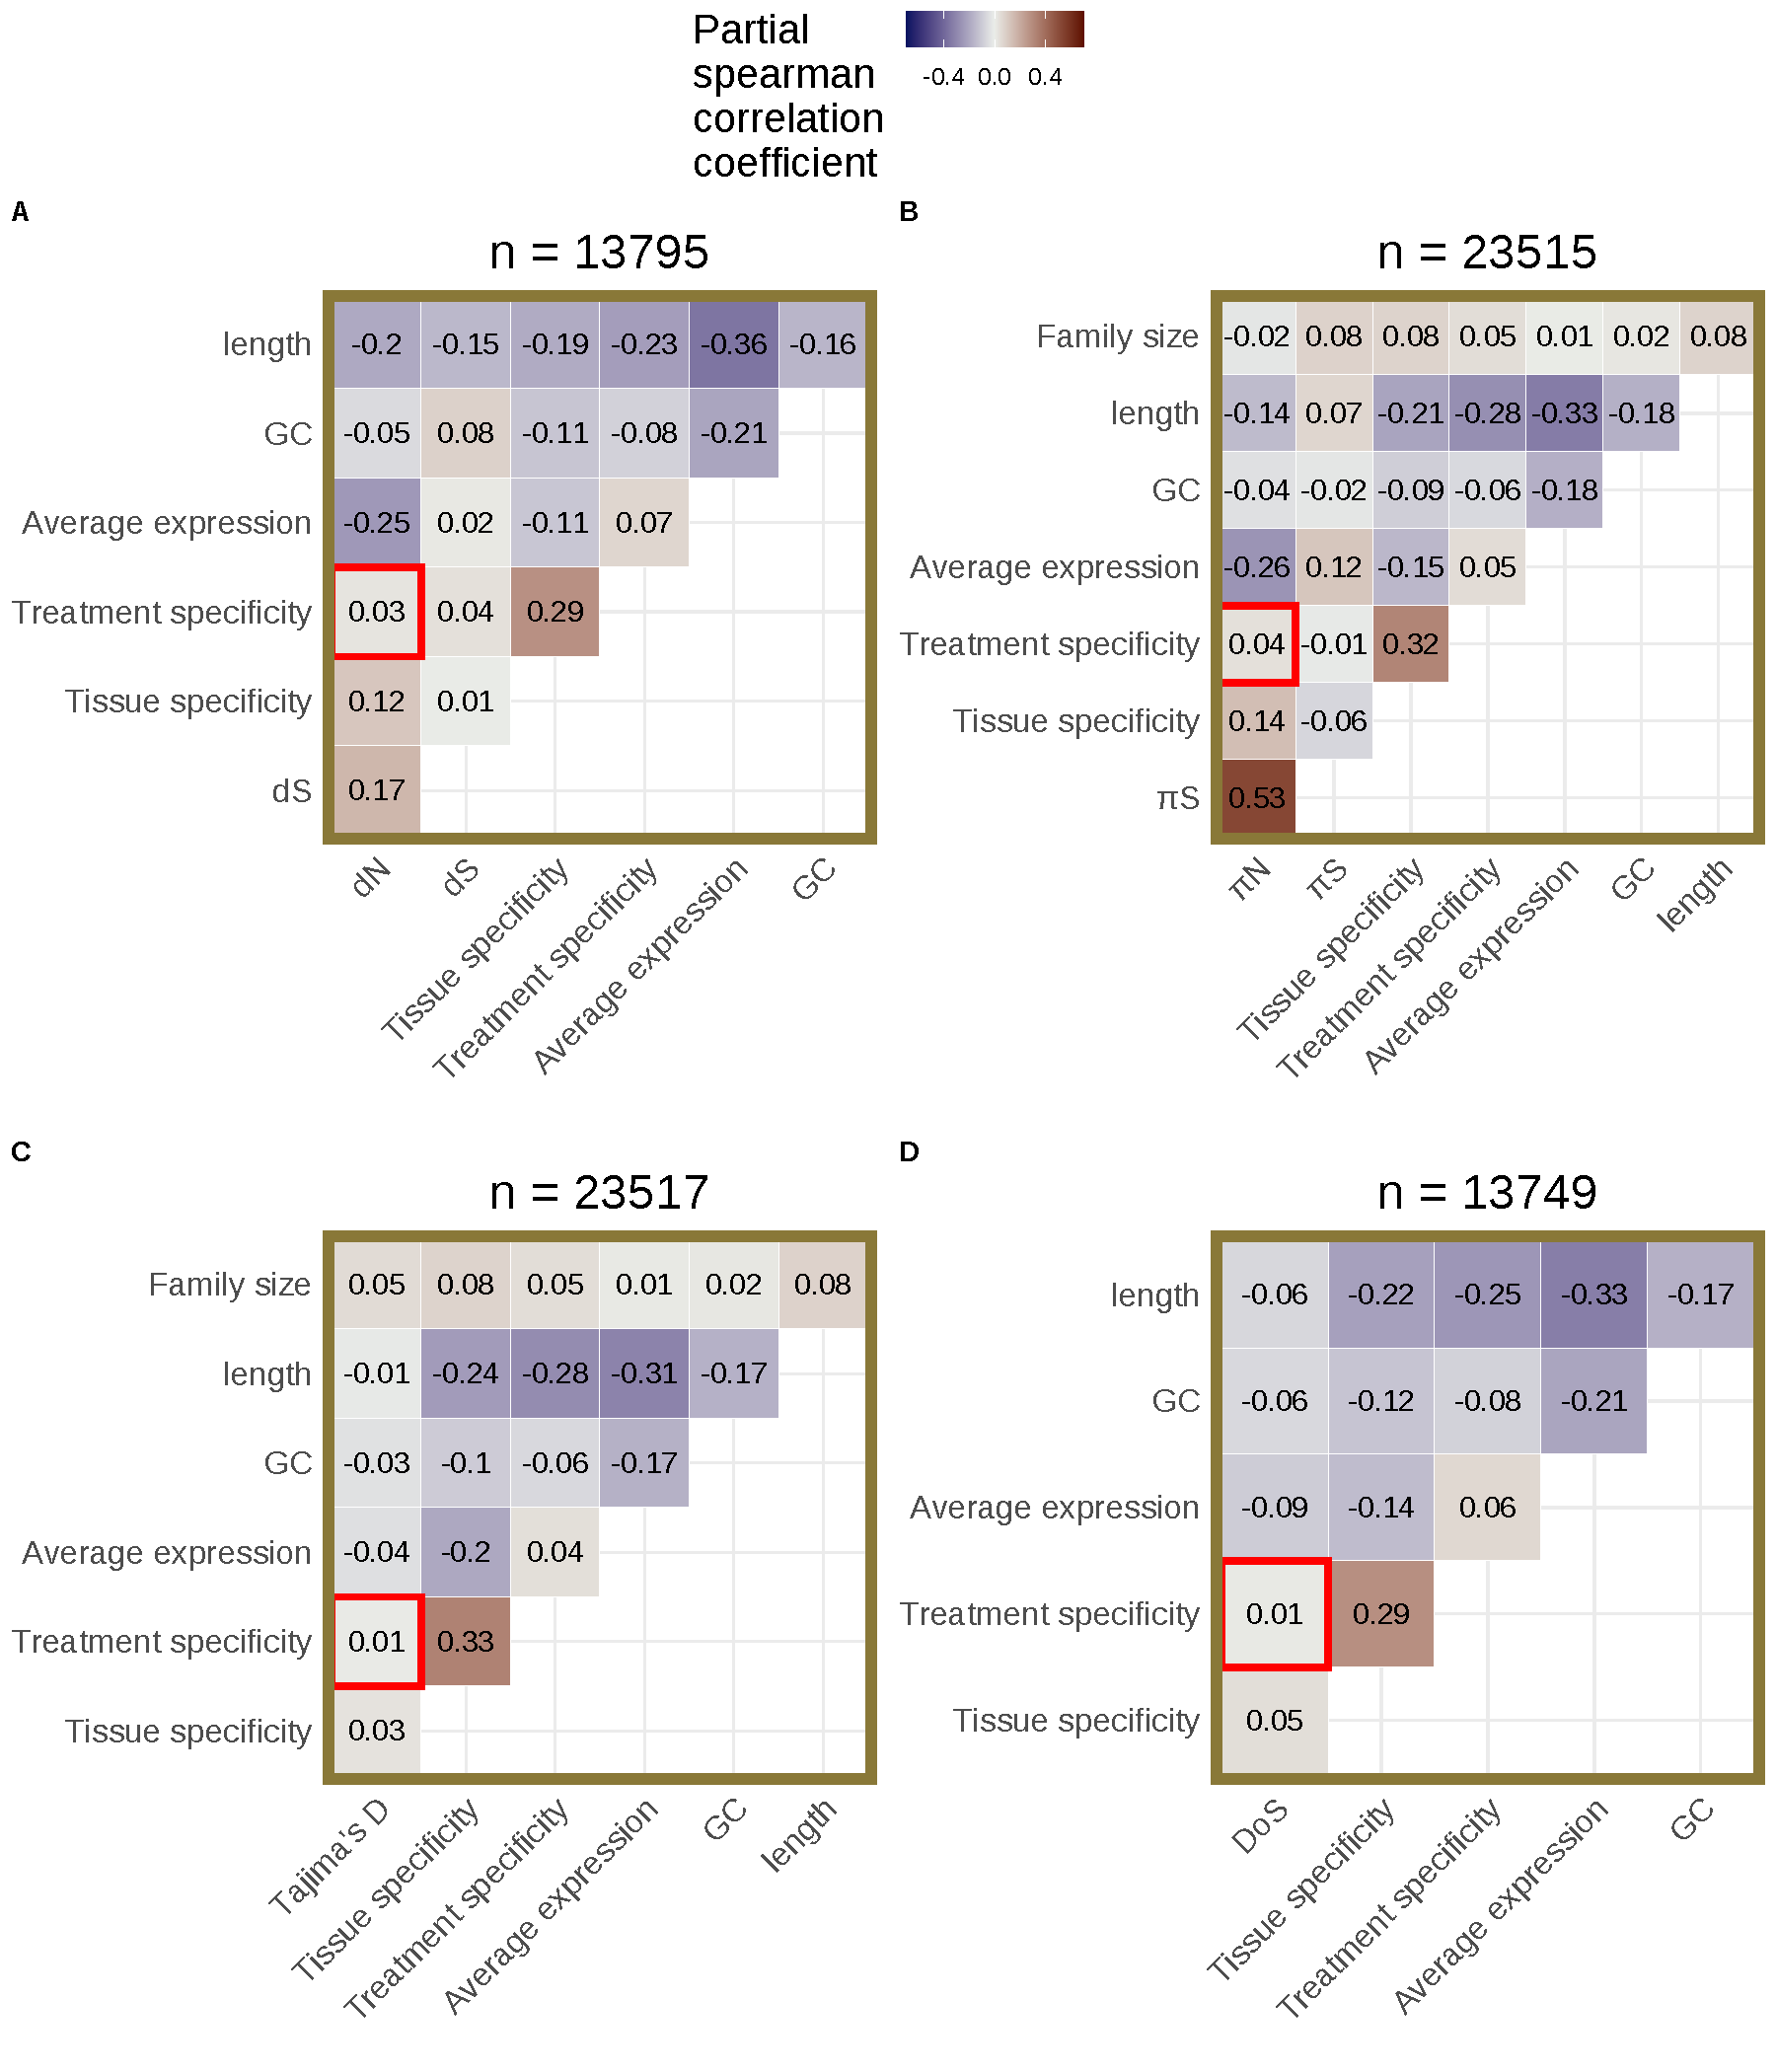
\includegraphics[width = \linewidth]{figures/appendix_a/partialCorrelations_fullyBalancedSubset_root_2023-02-22.pdf}
\caption{\textbf{Partial correlation analysis of root tissue on balanced data subset after SVA.} Partial correlations for (\textbf{A}) $dN$, (\textbf{B}) $\pi_N$, (\textbf{C}) Tajima's D, and (\textbf{D}) direction of selection (DoS) after applying SVA. Average expression and tissue specificity are calculated using only root tissue data. The number of genes included in each partial correlation analysis (n) is listed at the top of each heatmap.}%
\end{figure}

\begin{figure}[H]
\centering
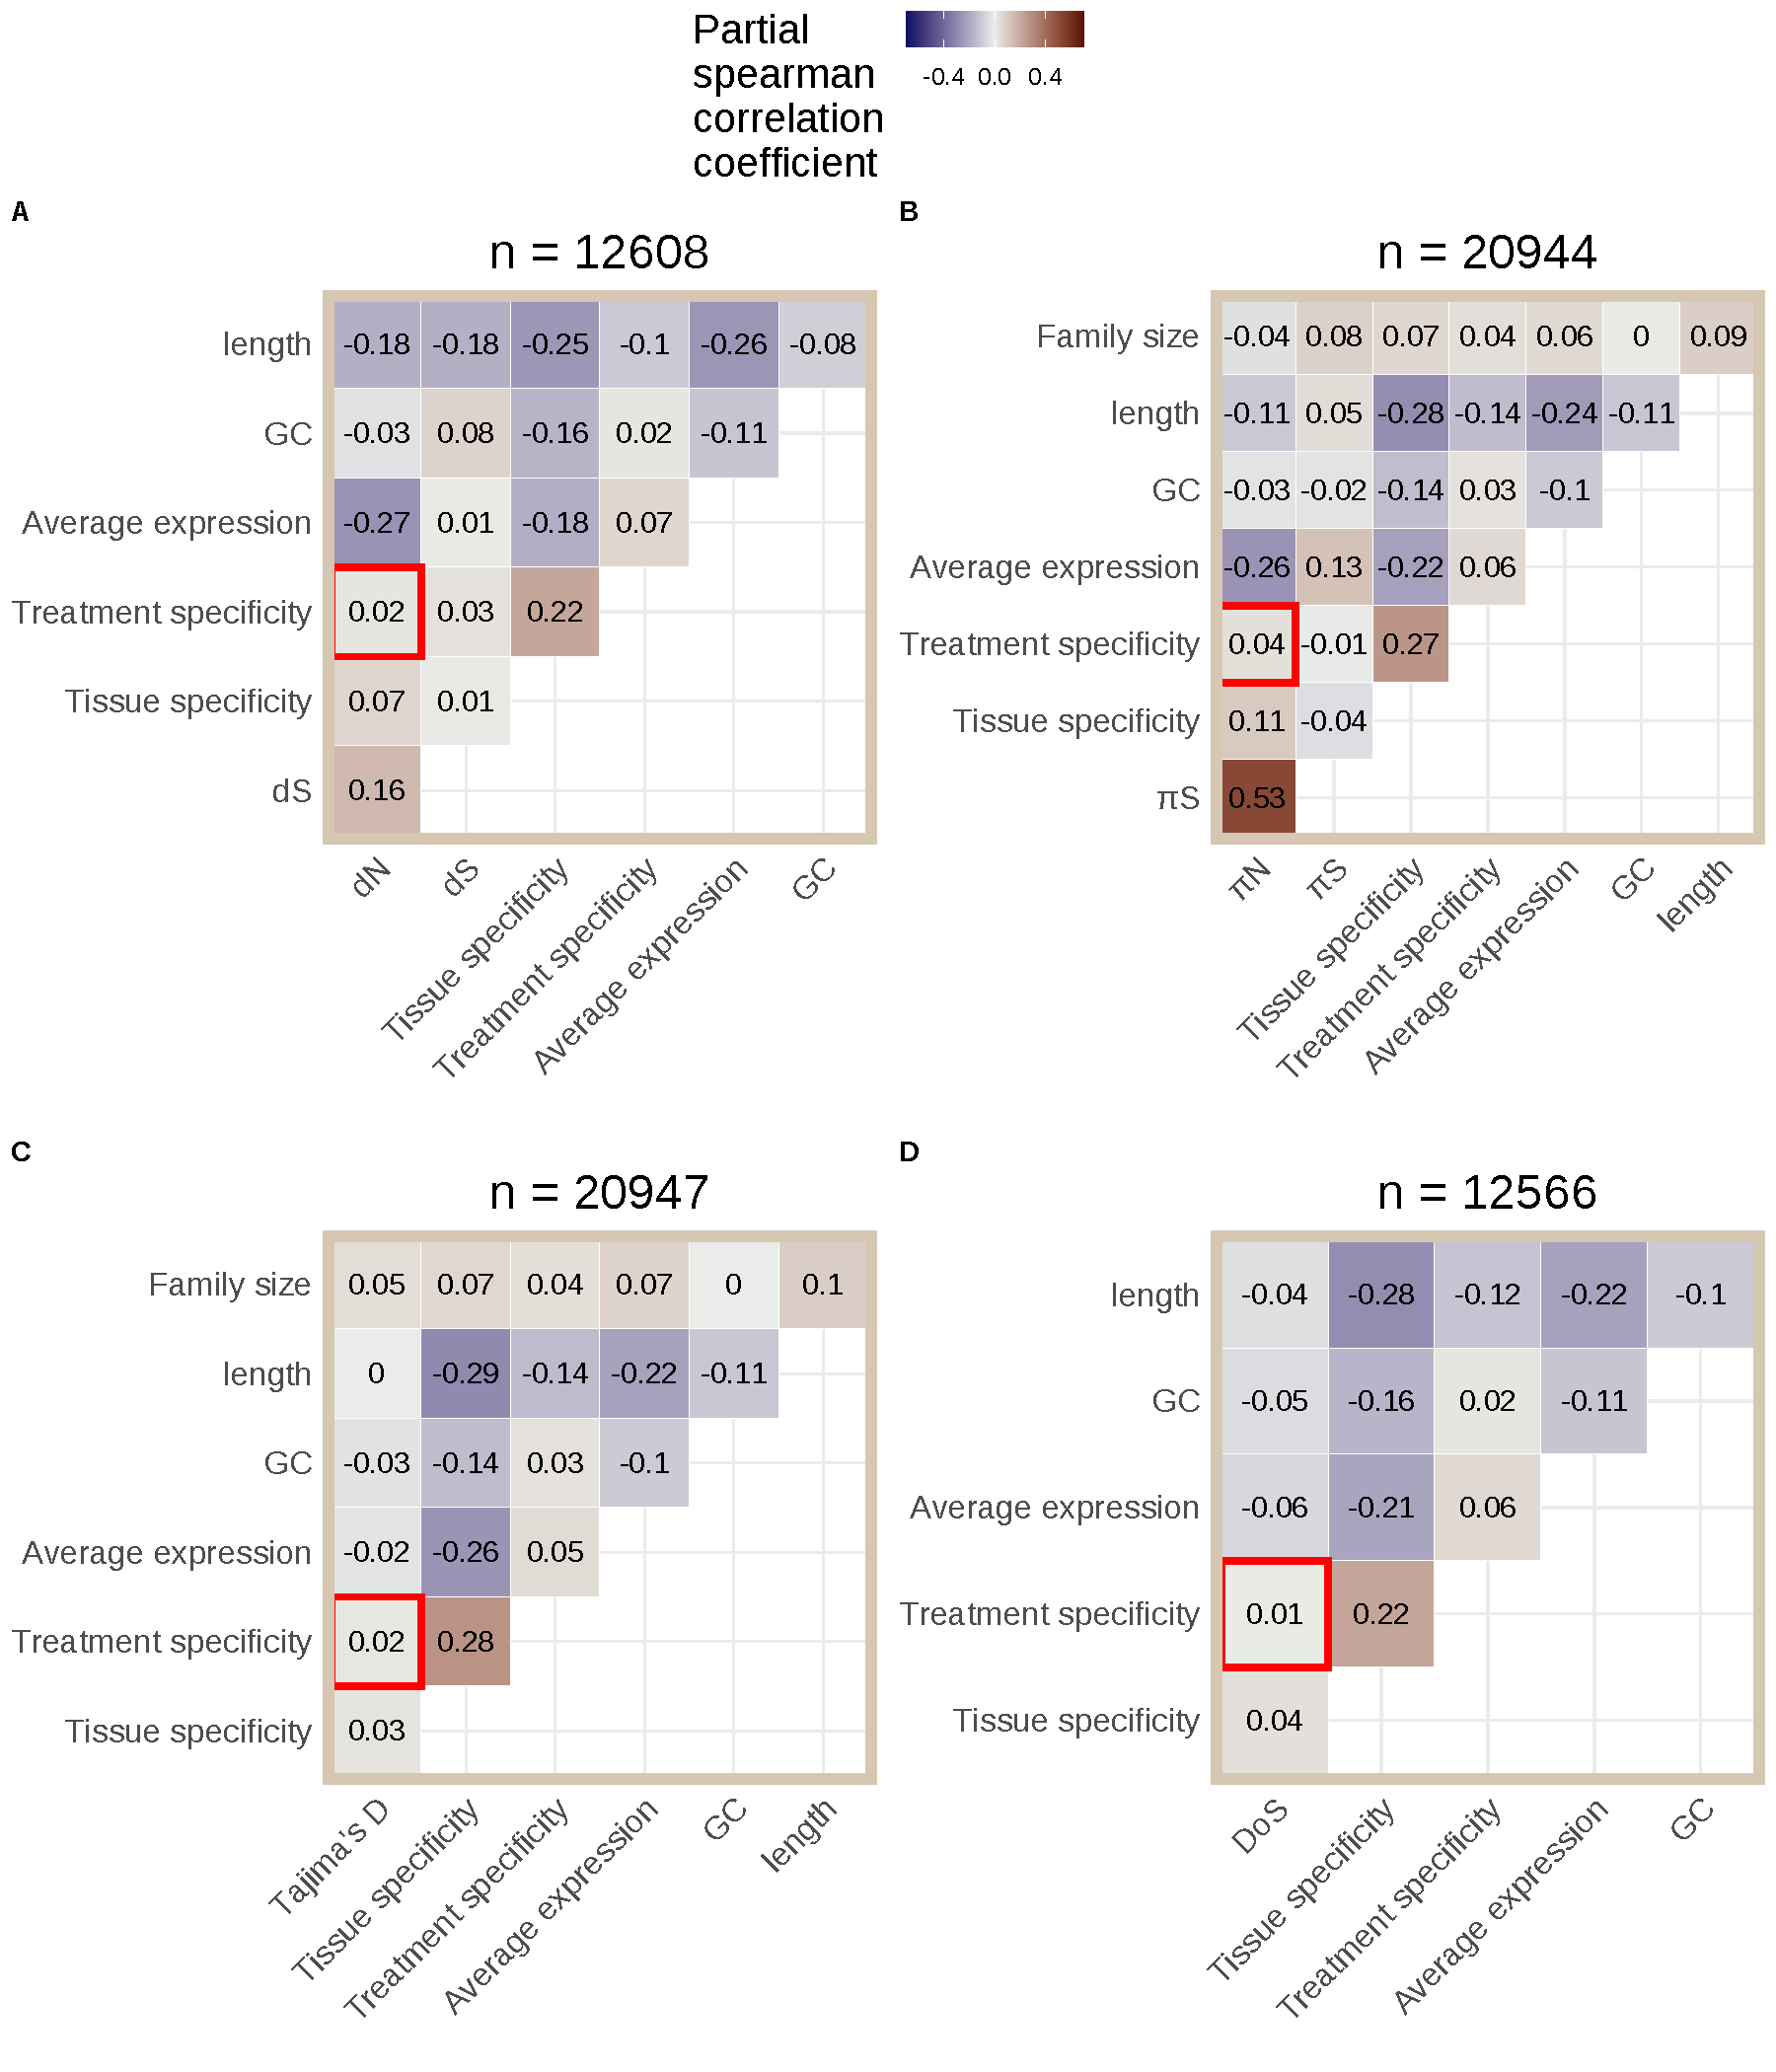
\includegraphics[width = \linewidth]{figures/appendix_a/partialCorrelations_fullyBalancedSubset_wholePlant_2023-02-22.pdf}
\caption{\textbf{Partial correlation analysis of whole plant tissue on balanced data subset after SVA.} Partial correlations for (\textbf{A}) $dN$, (\textbf{B}) $\pi_N$, (\textbf{C}) Tajima's D, and (\textbf{D}) direction of selection (DoS) after applying SVA. Average expression and tissue specificity are calculated using only whole plant tissue data. The number of genes included in each partial correlation analysis (n) is listed at the top of each heatmap.}%
\end{figure}


\begin{figure}[H]
\centering
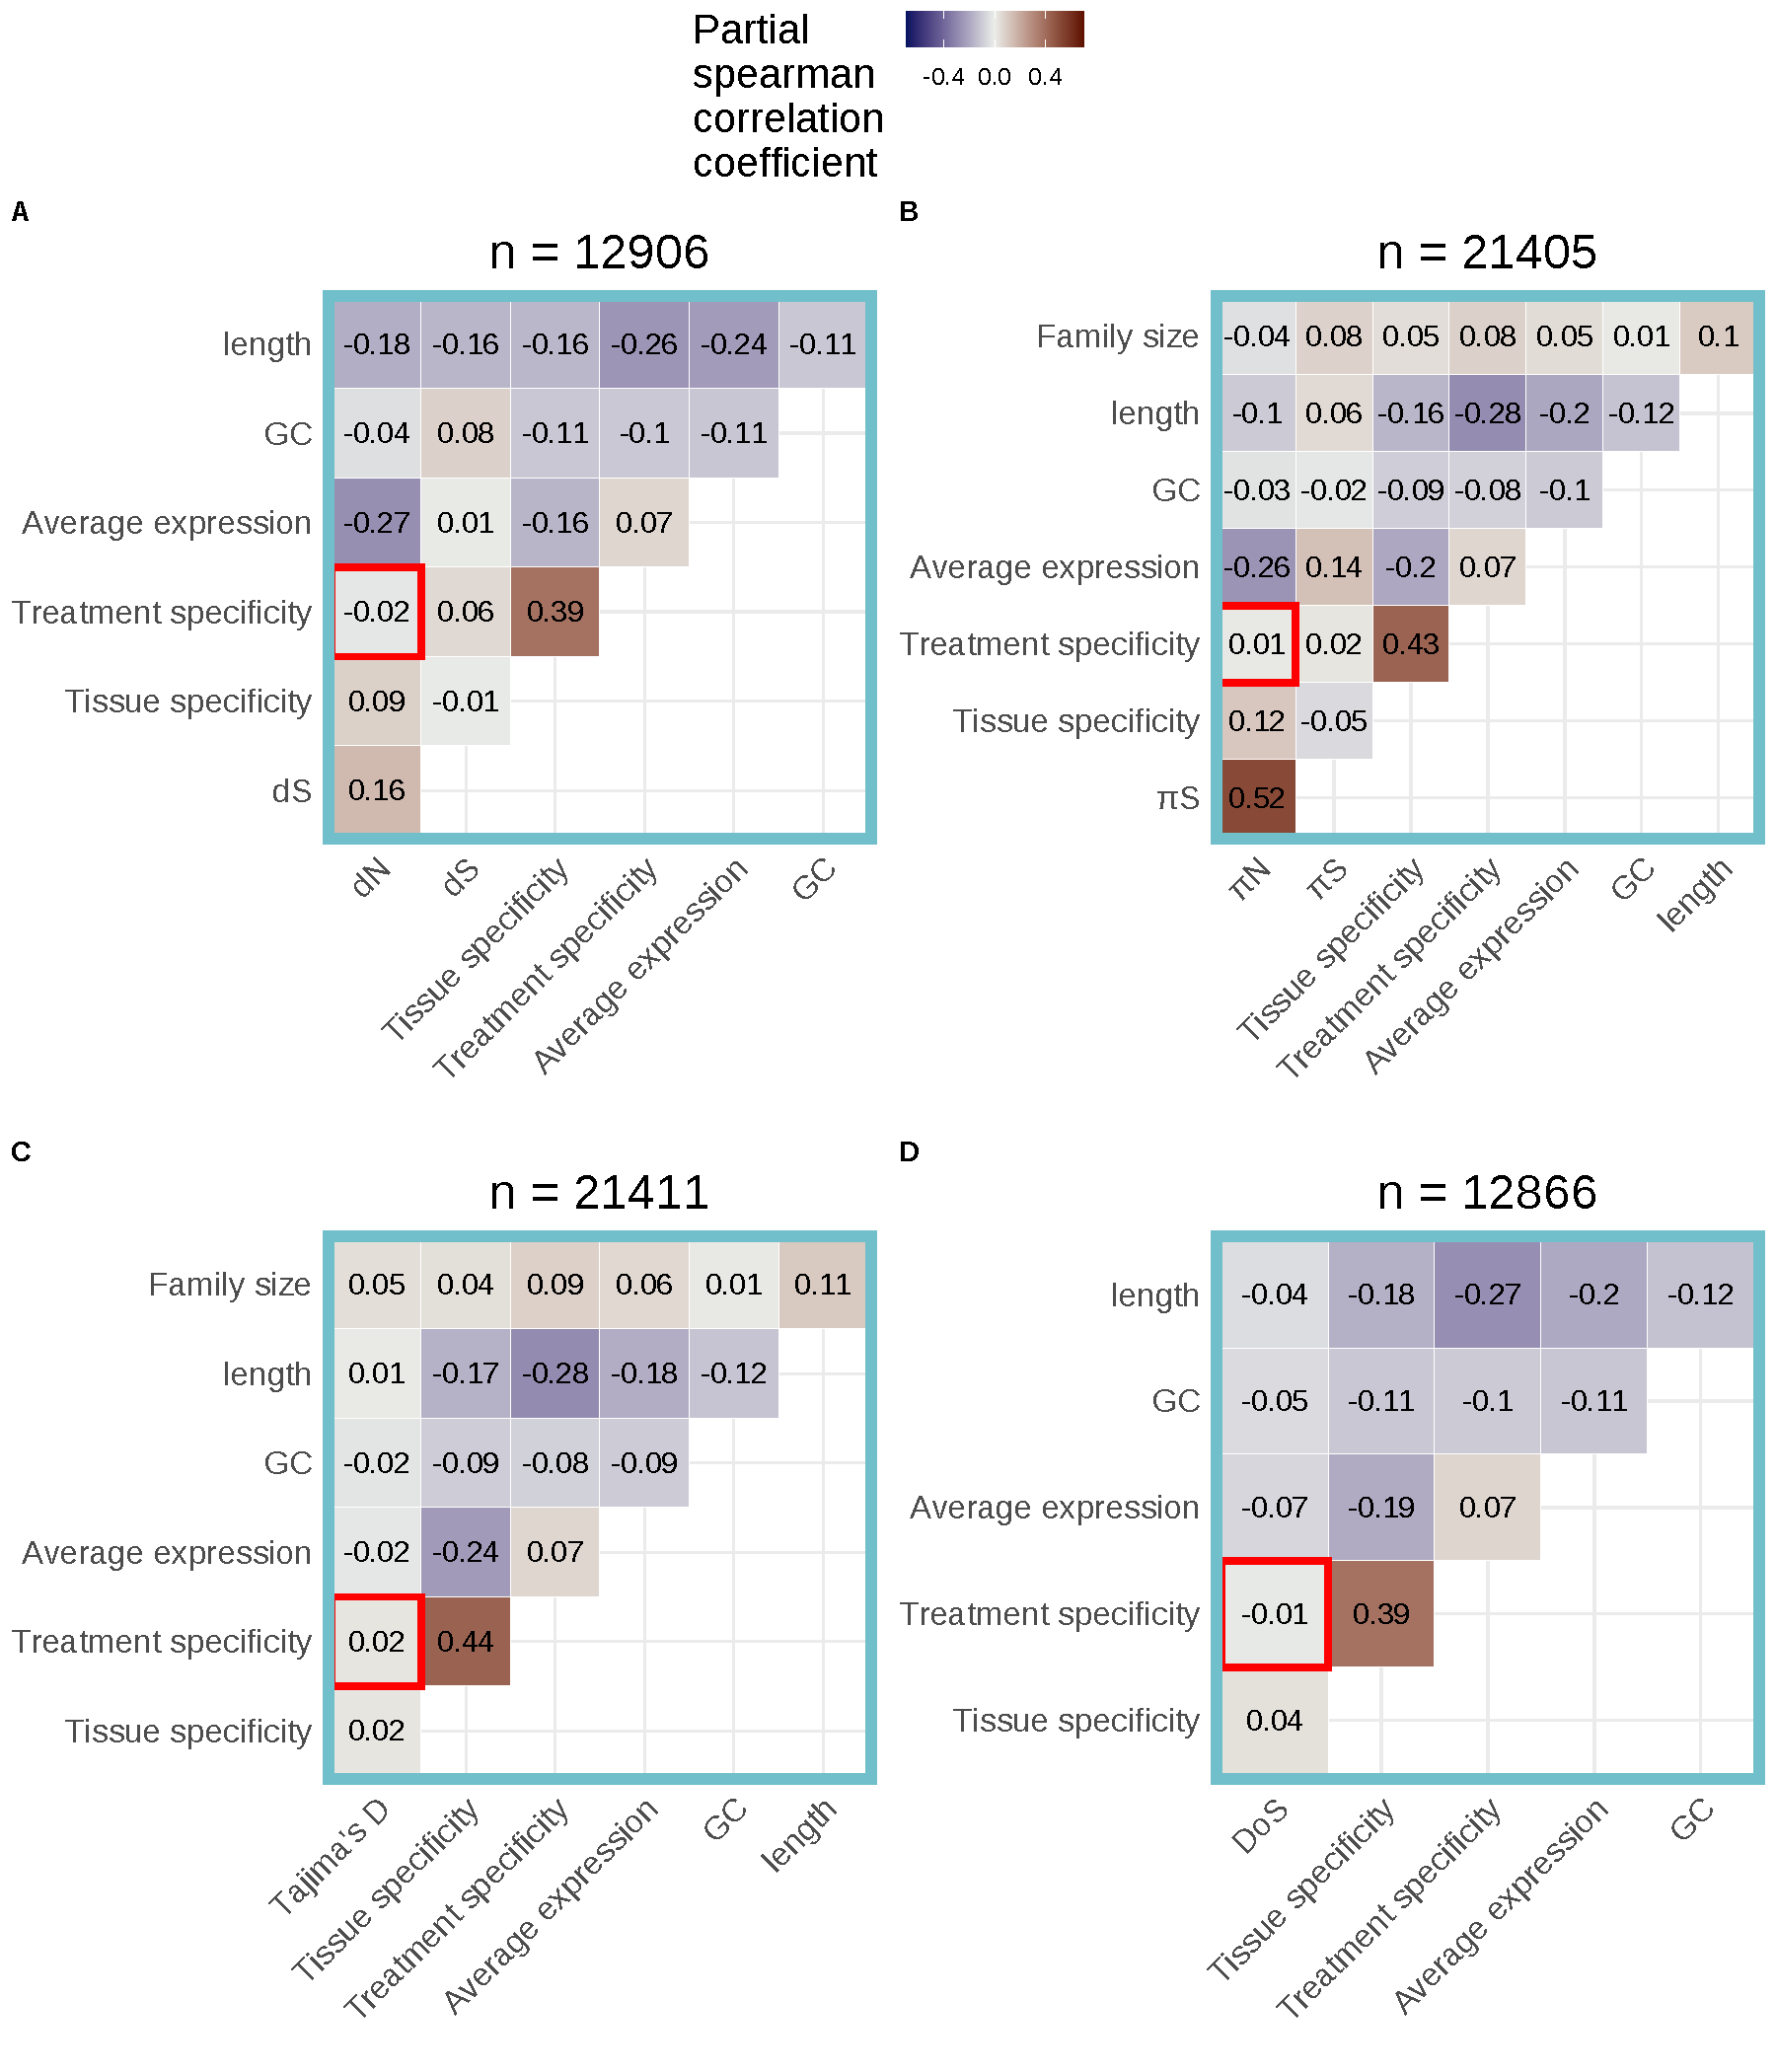
\includegraphics[width = \linewidth]{figures/appendix_a/partialCorrelations_fullyBalancedSubset_shoot_2023-02-22.pdf}
\caption{\textbf{Partial correlation analysis of shoot tissue on balanced data subset after SVA.} Partial correlations for (\textbf{A}) $dN$, (\textbf{B}) $\pi_N$, (\textbf{C}) Tajima's D, and (\textbf{D}) direction of selection (DoS) after applying SVA. Average expression and tissue specificity are calculated using only shoot tissue data. The number of genes included in each partial correlation analysis (n) is listed at the top of each heatmap.}%
\end{figure}

\begin{figure}[H]
\centering
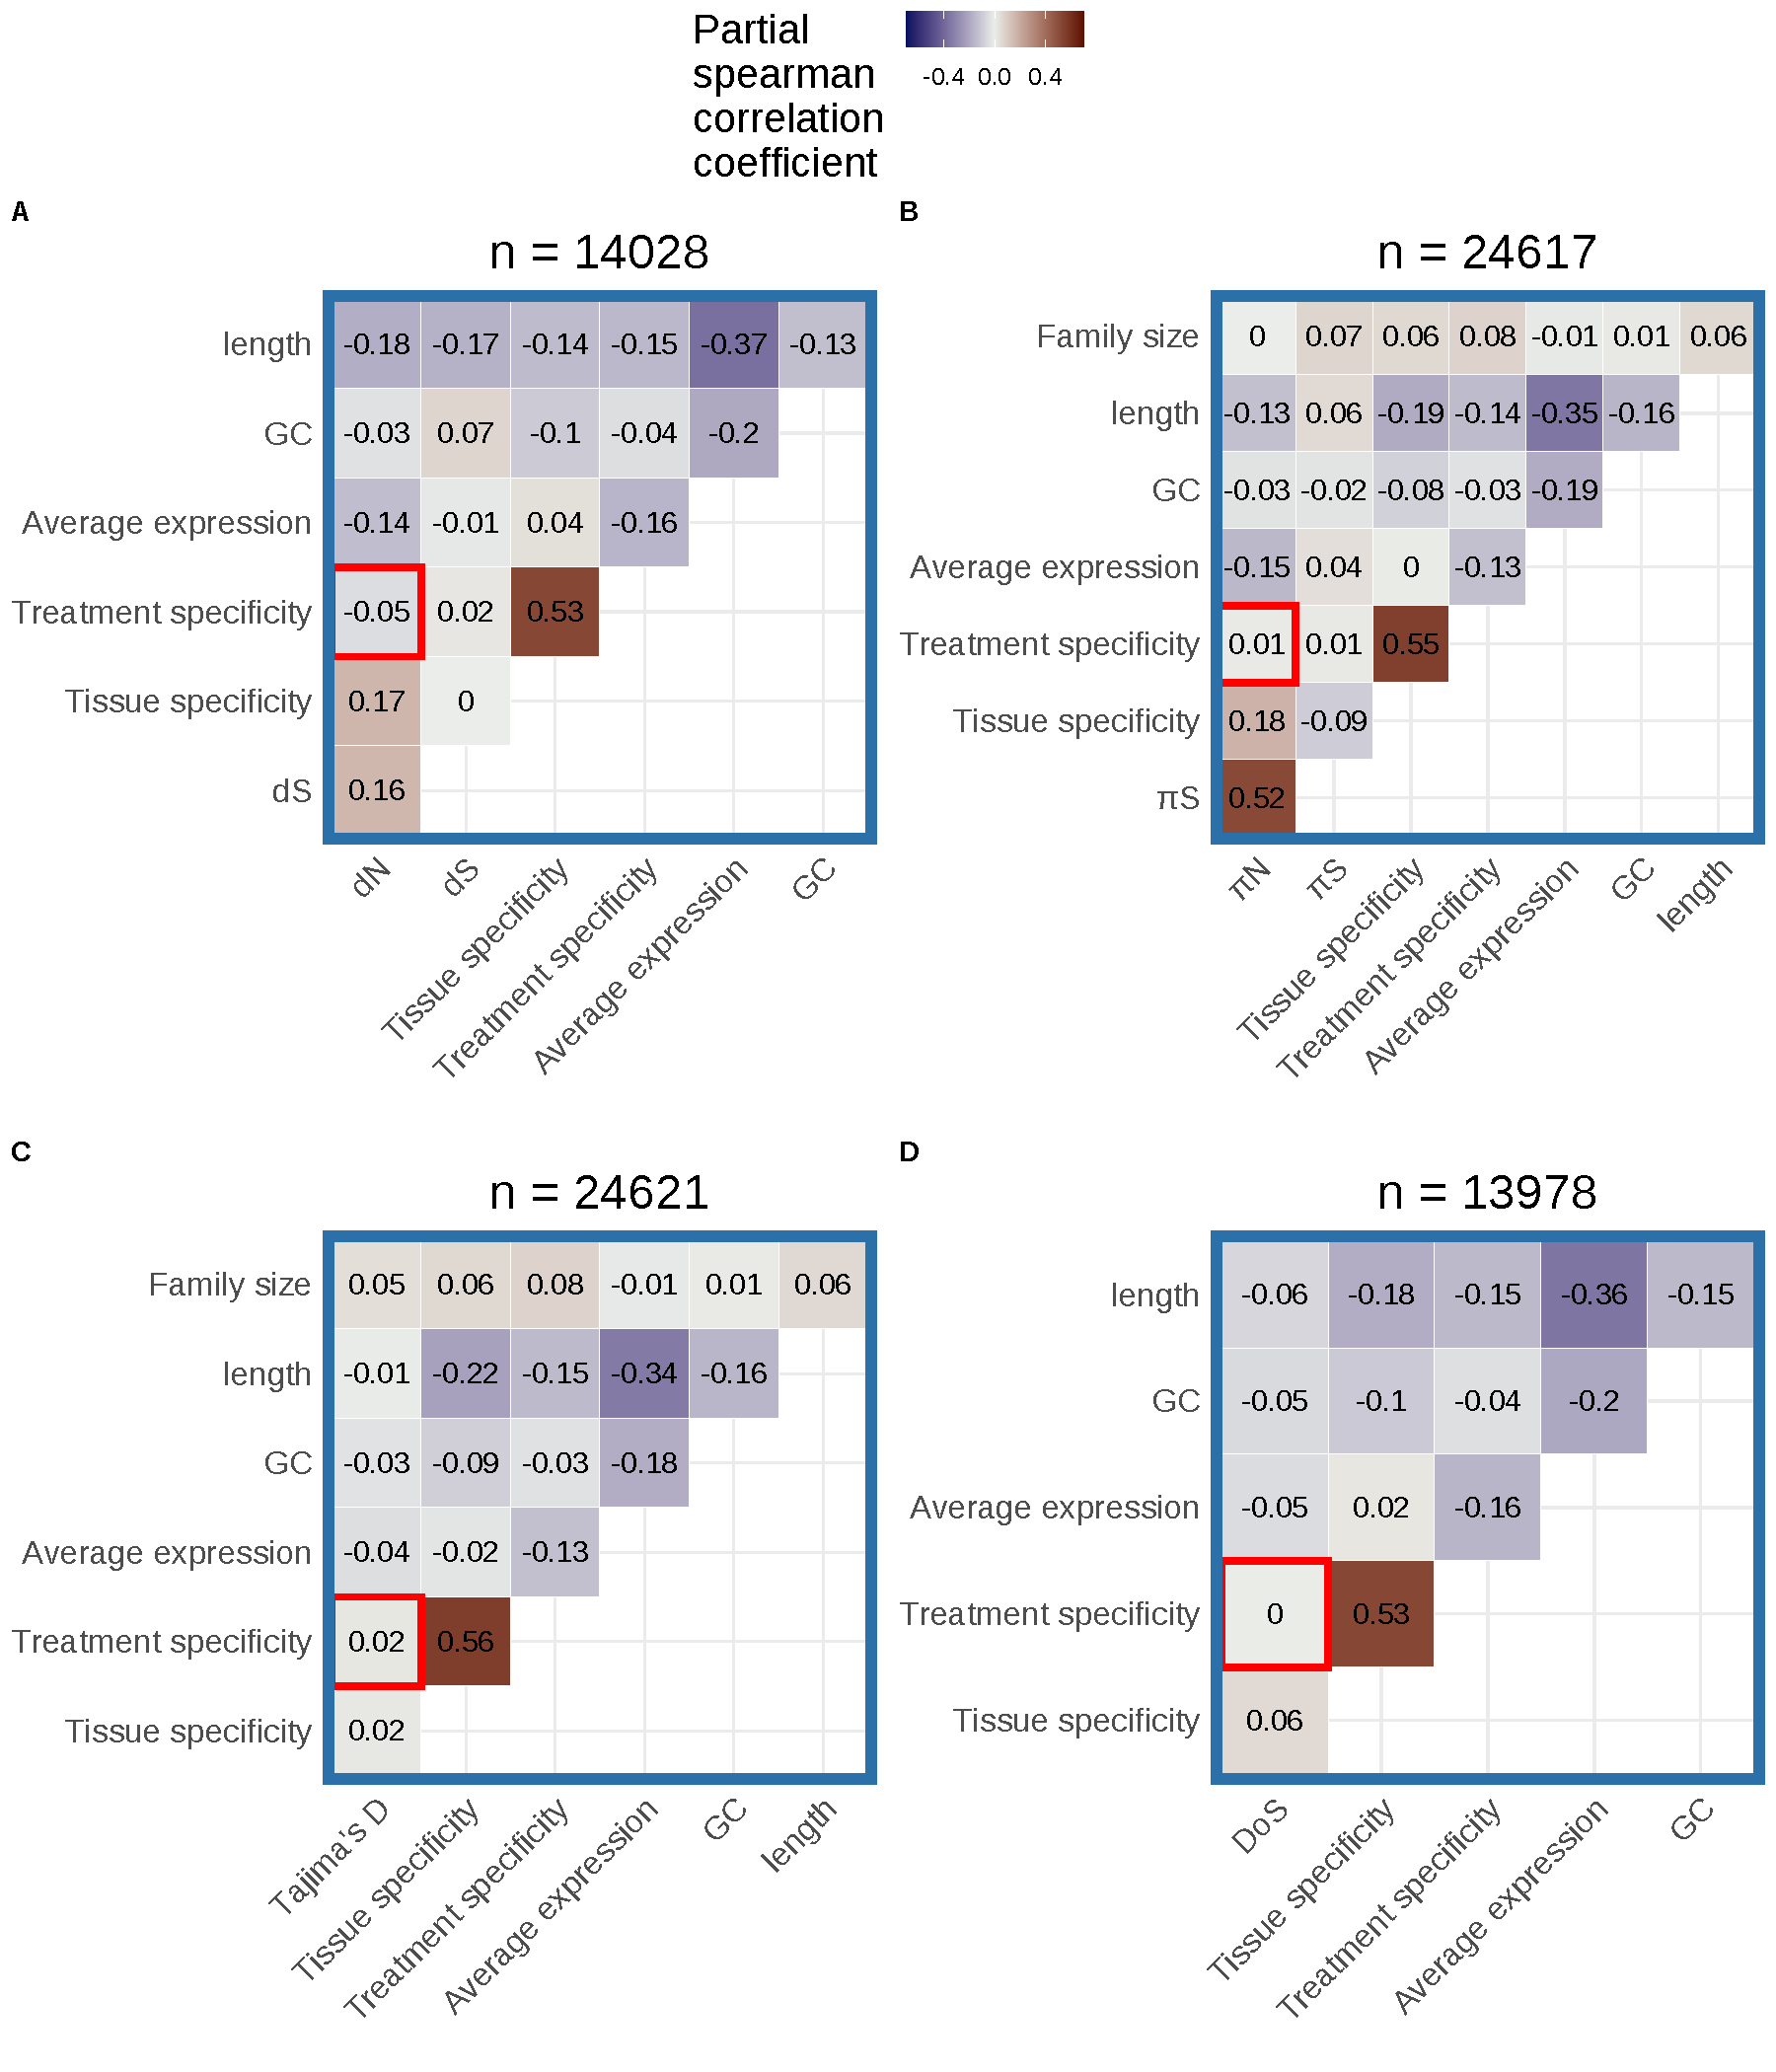
\includegraphics[width = \linewidth]{figures/appendix_a/partialCorrelations_fullyBalancedSubset_seed_2023-02-22.pdf}
\caption{\textbf{Partial correlation analysis of seed tissue on balanced data subset after SVA.} Partial correlations for (\textbf{A}) $dN$, (\textbf{B}) $\pi_N$, (\textbf{C}) Tajima's D, and (\textbf{D}) direction of selection (DoS) after applying SVA. Average expression and tissue specificity are calculated using only seed tissue data. The number of genes included in each partial correlation analysis (n) is listed at the top of each heatmap.}%
\end{figure}

\begin{figure}[H]
\centering
\includegraphics[width = \linewidth]{figures/appendix_a/partialCorrelations_fullyBalancedSubset_flowerORfruit_2023-02-22.pdf}
\caption{\textbf{Partial correlation analysis of fruit or flower tissue on balanced data subset after SVA.} Partial correlations for (\textbf{A}) $dN$, (\textbf{B}) $\pi_N$, (\textbf{C}) Tajima's D, and (\textbf{D}) direction of selection (DoS) after applying SVA. Average expression and tissue specificity are calculated using only fruit and flower tissue data. The number of genes included in each partial correlation analysis (n) is listed at the top of each heatmap.}%
\end{figure}

\subsection*{Effect of omitting low-expression values on treatment-specificity vs expression level correlation}

\begin{figure}[H]
\centering
\includegraphics[width = \linewidth]{figures/appendix_a/root_treatmentSpecificityVsAverageExpression_withVsWithoutZeros.pdf}
\caption{\textbf{Treatment specificity vs average expression correlation in root tissue.} Correlation between average expression in transcripts per million (TPM) and treatment specificity of genes when low expression values ($< 5$ TPM) are included (\textbf{A}) vs excluded (\textbf{B}). Expression level and treatment specificity were calculated using only data from root tissue samples. Line is a smoothing line with 95 \% confidence intervals and values in parentheses give spearman correlation.}%
\end{figure}

\begin{figure}[H]
\centering
\includegraphics[width = \linewidth]{figures/appendix_a/plant_treatmentSpecificityVsAverageExpression_withVsWithoutZeros.pdf}
\caption{\textbf{Treatment specificity vs average expression correlation in whole plant tissue.} Correlation between average expression in transcripts per million (TPM) and treatment specificity of genes when low expression values ($< 5$ TPM) are included (\textbf{A}) vs excluded (\textbf{B}). Expression level and treatment specificity were calculated using only data from whole plant tissue samples. Line is a smoothing line with 95 \% confidence intervals and values in parentheses give spearman correlation.}%
\end{figure}

\begin{figure}[H]
\centering
\includegraphics[width = \linewidth]{figures/appendix_a/shoot_treatmentSpecificityVsAverageExpression_withVsWithoutZeros.pdf}
\caption{\textbf{Treatment specificity vs average expression correlation in shoot tissue.} Correlation between average expression in transcripts per million (TPM) and treatment specificity of genes when low expression values ($< 5$ TPM) are included (\textbf{A}) vs excluded (\textbf{B}). Expression level and treatment specificity were calculated using only data from shoot tissue samples. Line is a smoothing line with 95 \% confidence intervals and values in parentheses give spearman correlation.}%
\end{figure}

\begin{figure}[H]
\centering
\includegraphics[width = \linewidth]{figures/appendix_a/seed_treatmentSpecificityVsAverageExpression_withVsWithoutZeros.pdf}
\caption{\textbf{Treatment specificity vs average expression correlation in seed tissue.} Correlation between average expression in transcripts per million (TPM) and treatment specificity of genes when low expression values ($< 5$ TPM) are included (\textbf{A}) vs excluded (\textbf{B}). Expression level and treatment specificity were calculated using only data from seed tissue samples. Line is a smoothing line with 95 \% confidence intervals and values in parentheses give spearman correlation.}%
\end{figure}

\begin{figure}[H]
\centering
\includegraphics[width = \linewidth]{figures/appendix_a/flower_treatmentSpecificityVsAverageExpression_withVsWithoutZeros.pdf}
\caption{\textbf{Treatment specificity vs average expression correlation in fruit or flower tissue.} Correlation between average expression in transcripts per million (TPM) and treatment specificity of genes when low expression values ($< 5$ TPM) are included (\textbf{A}) vs excluded (\textbf{B}). Expression level and treatment specificity were calculated using only data from fruit and flower tissue samples. Line is a smoothing line with 95 \% confidence intervals and values in parentheses give spearman correlation.}%
\end{figure}

\subsection*{Simulating level-specificity correlation}

\begin{figure}[H]
\centering
\includegraphics[width = \linewidth]{figures/appendix_a/SimulationResults.pdf}
\caption{\textbf{Violin plot of correlations between expression specificity and expression level across 1000 simulated expression matrices.} In the two different simulations shown here, expression level was quantified either as average expression across all samples or average expression across samples with expression values $>$ 0. Each expression matrix was simulated by sampling from a zero-inflated negative binomial distribution.}%
\end{figure}

\newpage

\begin{comment}
\section*{APPENDIX - Deprecated}
\addcontentsline{toc}{subsection}{APPENDIX B: SUPPLEMENTAL TABLES FOR CHAPTER 1}

\setcounter{table}{0}
\renewcommand{\tablename}{Table} 
\renewcommand{\thetable}{B.\Alph{table}} 

\subsection*{Leaf tissue}

\begin{landscape}
\begin{table}[H]
    \centering
    \begin{tabularx}{\linewidth}{|L|L|L|L|L|L|L|L|}
    \hline
        \textbf{} & \textbf{dN} & \textbf{dS} & \textbf{Tissue specificity} & \textbf{Treatment specificity} & \textbf{Average expression} & \textbf{GC} & \textbf{length} \\ \hline
        \textbf{dN} & 0 & 6.86196E-96 & 1.6574E-42 & 7.58333E-31 & 2.0557E-122 & 0.000178339 & 4.6047E-111 \\ \hline
        \textbf{dS} & 6.86196E-96 & 0 & 0.019644077 & 5.01104E-10 & 0.012375514 & 1.51264E-21 & 1.04221E-68 \\ \hline
        \textbf{Tissue specificity} & 1.6574E-42 & 0.019644077 & 0 & 0 & 8.17935E-37 & 1.23179E-45 & 2.37759E-78 \\ \hline
        \textbf{Treatment specificity} & 7.58333E-31 & 5.01104E-10 & 0 & 0 & 3.86873E-25 & 0.099815364 & 1.03409E-73 \\ \hline
        \textbf{Average expression} & 2.0557E-122 & 0.012375514 & 8.17935E-37 & 3.86873E-25 & 0 & 1.81806E-70 & 0 \\ \hline
        \textbf{GC} & 0.000178339 & 1.51264E-21 & 1.23179E-45 & 0.099815364 & 1.81806E-70 & 0 & 4.58314E-51 \\ \hline
        \textbf{length} & 4.6047E-111 & 1.04221E-68 & 2.37759E-78 & 1.03409E-73 & 0 & 4.58314E-51 & 0 \\ \hline
    \end{tabularx}
    \caption{P-values for partial correlations with dN in leaf tissue without batch correction}
\end{table}

\begin{table}[H]
    \centering
    \begin{tabularx}{\linewidth}{|L|L|L|L|L|L|L|L|}
    \hline
        \textbf{} & \textbf{πN} & \textbf{πS} & \textbf{Tissue specificity} & \textbf{Treatment specificity} & \textbf{Average expression} & \textbf{GC} & \textbf{length} & \textbf{Family size } \\ \hline
        \textbf{πN} & 0 & 0 & 7.4955E-113 & 1.22872E-62 & 2.7811E-175 & 0.007635805 & 1.01377E-96 & 0.000855273  \\ \hline
        \textbf{πS} & 0 & 0 & 1.27798E-34 & 0.00029424 & 4.71787E-60 & 0.000902879 & 4.14719E-43 & 4.37897E-23  \\ \hline
        \textbf{Tissue specificity} & 7.4955E-113 & 1.27798E-34 & 0 & 0 & 1.4182E-130 & 2.683E-60 & 1.4306E-153 & 2.86128E-15  \\ \hline
        \textbf{Treatment specificity} & 1.22872E-62 & 0.00029424 & 0 & 0 & 1.77625E-68 & 0.189284279 & 4.0213E-268 & 6.26814E-84  \\ \hline
        \textbf{Average expression} & 2.7811E-175 & 4.71787E-60 & 1.4182E-130 & 1.77625E-68 & 0 & 7.791E-108 & 0 & 2.99157E-30  \\ \hline
        \textbf{GC} & 0.007635805 & 0.000902879 & 2.683E-60 & 0.189284279 & 7.791E-108 & 0 & 4.6984E-144 & 2.85735E-08  \\ \hline
        \textbf{length} & 1.01377E-96 & 4.14719E-43 & 1.4306E-153 & 4.0213E-268 & 0 & 4.6984E-144 & 0 & 2.7895E-71  \\ \hline
        \textbf{Family size} & 0.000855273 & 4.37897E-23 & 2.86128E-15 & 6.26814E-84 & 2.99157E-30 & 2.85735E-08 & 2.7895E-71 & 0  \\ \hline
    \end{tabularx}
    \caption{P-values for partial correlations with $\pi_N$ in leaf tissue without batch correction}
\end{table}
\end{landscape}

\begin{table}[H]
    \centering
    \resizebox{\textwidth}{!}{\begin{tabular}{|l|l|l|l|l|l|l|l|}
    \hline
        \textbf{} & \textbf{Tajima's D} & \textbf{Tissue specificity} & \textbf{Treatment specificity} & \textbf{Average expression} & \textbf{GC} & \textbf{length} & \textbf{Family size} \\ \hline
        \textbf{Tajima's D} & 0 & 0.062983693 & 3.10049E-07 & 0.38323534 & 0.000604045 & 0.015675353 & 1.33307E-15 \\ \hline
        \textbf{Tissue specificity} & 0.062983693 & 0 & 0 & 2.0133E-184 & 5.22161E-64 & 4.3932E-197 & 5.34588E-17 \\ \hline
        \textbf{Treatment specificity} & 3.10049E-07 & 0 & 0 & 2.8342E-50 & 0.344365339 & 0 & 4.25828E-90 \\ \hline
        \textbf{Average expression} & 0.38323534 & 2.0133E-184 & 2.8342E-50 & 0 & 1.5768E-107 & 0 & 3.50717E-29 \\ \hline
        \textbf{GC} & 0.000604045 & 5.22161E-64 & 0.344365339 & 1.5768E-107 & 0 & 5.3053E-143 & 2.65613E-07 \\ \hline
        \textbf{length} & 0.015675353 & 4.3932E-197 & 0 & 0 & 5.3053E-143 & 0 & 7.42762E-70 \\ \hline
        \textbf{Family size} & 1.33307E-15 & 5.34588E-17 & 4.25828E-90 & 3.50717E-29 & 2.65613E-07 & 7.42762E-70 & 0 \\ \hline
    \end{tabular}}
    \caption{P-values for partial correlations with Tajima's D in leaf tissue without batch correction}
\end{table}

\begin{table}[H]
    \centering
    \resizebox{\textwidth}{!}{\begin{tabular}{|l|l|l|l|l|l|l|}
    \hline
        \textbf{} & \textbf{DoS} & \textbf{Tissue specificity} & \textbf{Treatment specificity} & \textbf{Average expression} & \textbf{GC} & \textbf{length} \\ \hline
        \textbf{DoS} & 0 & 2.71611E-08 & 2.33534E-06 & 1.77197E-05 & 2.01301E-09 & 1.13481E-11 \\ \hline
        \textbf{Tissue specificity} & 2.71611E-08 & 0 & 0 & 2.05484E-53 & 4.88089E-47 & 5.5627E-105 \\ \hline
        \textbf{Treatment specificity} & 2.33534E-06 & 0 & 0 & 5.48075E-16 & 0.269561212 & 6.974E-109 \\ \hline
        \textbf{Average expression} & 1.77197E-05 & 2.05484E-53 & 5.48075E-16 & 0 & 6.881E-70 & 0 \\ \hline
        \textbf{GC} & 2.01301E-09 & 4.88089E-47 & 0.269561212 & 6.881E-70 & 0 & 2.37195E-64 \\ \hline
        \textbf{length} & 1.13481E-11 & 5.5627E-105 & 6.974E-109 & 0 & 2.37195E-64 & 0 \\ \hline
    \end{tabular}}
    \caption{P-values for partial correlations with DoS in leaf tissue without batch correction}
\end{table}

\subsection*{Root tissue}

\begin{table}[H]
    \centering
    \resizebox{\textwidth}{!}{\begin{tabular}{|l|l|l|l|l|l|l|l|}
    \hline
        \textbf{} & \textbf{dN} & \textbf{dS} & \textbf{Tissue specificity} & \textbf{Treatment specificity} & \textbf{Average expression} & \textbf{GC} & \textbf{length} \\ \hline
        \textbf{dN} & 0 & 2.22597E-89 & 1.82195E-38 & 6.13192E-26 & 1.1581E-224 & 9.25632E-09 & 1.1379E-105 \\ \hline
        \textbf{dS} & 2.22597E-89 & 0 & 0.187865901 & 1.03692E-06 & 0.019281255 & 2.57225E-21 & 1.02315E-70 \\ \hline
        \textbf{Tissue specificity} & 1.82195E-38 & 0.187865901 & 0 & 0 & 2.572E-56 & 1.74295E-58 & 9.54881E-58 \\ \hline
        \textbf{Treatment specificity} & 6.13192E-26 & 1.03692E-06 & 0 & 0 & 3.87708E-71 & 0.489801928 & 1.177E-173 \\ \hline
        \textbf{Average expression} & 1.1581E-224 & 0.019281255 & 2.572E-56 & 3.87708E-71 & 0 & 2.55528E-98 & 1.2784E-295 \\ \hline
        \textbf{GC} & 9.25632E-09 & 2.57225E-21 & 1.74295E-58 & 0.489801928 & 2.55528E-98 & 0 & 1.33182E-47 \\ \hline
        \textbf{length} & 1.1379E-105 & 1.02315E-70 & 9.54881E-58 & 1.177E-173 & 1.2784E-295 & 1.33182E-47 & 0 \\ \hline
    \end{tabular}}
    \caption{P-values for partial correlations with dN in root tissue without batch correction}
\end{table}

\begin{table}[H]
    \centering
    \resizebox{\textwidth}{!}{\begin{tabular}{|l|l|l|l|l|l|l|l|l|}
    \hline
        \textbf{} & \textbf{πN} & \textbf{πS} & \textbf{Tissue specificity} & \textbf{Treatment specificity} & \textbf{Average expression} & \textbf{GC} & \textbf{length} & \textbf{Family size } \\ \hline
        \textbf{πN} & 0 & 0 & 2.11895E-85 & 3.16325E-51 & 0 & 3.0131E-07 & 9.97908E-82 & 0.186992611  \\ \hline
        \textbf{πS} & 0 & 0 & 8.93404E-26 & 3.94926E-05 & 1.19128E-93 & 0.00298918 & 2.36866E-28 & 1.32255E-34  \\ \hline
        \textbf{Tissue specificity} & 2.11895E-85 & 8.93404E-26 & 0 & 0 & 2.3997E-153 & 1.20532E-68 & 1.4936E-123 & 2.48857E-23  \\ \hline
        \textbf{Treatment specificity} & 3.16325E-51 & 3.94926E-05 & 0 & 0 & 5.57076E-53 & 0.167967439 & 0 & 4.1853E-25  \\ \hline
        \textbf{Average expression} & 0 & 1.19128E-93 & 2.3997E-153 & 5.57076E-53 & 0 & 1.0285E-121 & 0 & 0.062925043  \\ \hline
        \textbf{GC} & 3.0131E-07 & 0.00298918 & 1.20532E-68 & 0.167967439 & 1.0285E-121 & 0 & 4.7362E-114 & 0.001378946  \\ \hline
        \textbf{length} & 9.97908E-82 & 2.36866E-28 & 1.4936E-123 & 0 & 0 & 4.7362E-114 & 0 & 2.34334E-40  \\ \hline
        \textbf{Family size} & 0.186992611 & 1.32255E-34 & 2.48857E-23 & 4.1853E-25 & 0.062925043 & 0.001378946 & 2.34334E-40 & 0  \\ \hline
    \end{tabular}}
    \caption{P-values for partial correlations with $\pi_N$ in root tissue without batch correction}
\end{table}

\begin{table}[H]
    \centering
    \resizebox{\textwidth}{!}{\begin{tabular}{|l|l|l|l|l|l|l|l|}
    \hline
        \textbf{} & \textbf{Tajima's D} & \textbf{Tissue specificity} & \textbf{Treatment specificity} & \textbf{Average expression} & \textbf{GC} & \textbf{length} & \textbf{Family size} \\ \hline
        \textbf{Tajima's D} & 0 & 0.007161374 & 5.54795E-05 & 1.81448E-05 & 5.31962E-06 & 0.597755917 & 7.30727E-17 \\ \hline
        \textbf{Tissue specificity} & 0.007161374 & 0 & 0 & 4.9906E-240 & 2.58965E-74 & 2.0279E-154 & 3.3281E-22 \\ \hline
        \textbf{Treatment specificity} & 5.54795E-05 & 0 & 0 & 4.59195E-32 & 0.449234494 & 0 & 7.63756E-26 \\ \hline
        \textbf{Average expression} & 1.81448E-05 & 4.9906E-240 & 4.59195E-32 & 0 & 6.9848E-117 & 0 & 0.019056833 \\ \hline
        \textbf{GC} & 5.31962E-06 & 2.58965E-74 & 0.449234494 & 6.9848E-117 & 0 & 1.1794E-109 & 0.004771647 \\ \hline
        \textbf{length} & 0.597755917 & 2.0279E-154 & 0 & 0 & 1.1794E-109 & 0 & 6.14377E-42 \\ \hline
        \textbf{Family size} & 7.30727E-17 & 3.3281E-22 & 7.63756E-26 & 0.019056833 & 0.004771647 & 6.14377E-42 & 0 \\ \hline
    \end{tabular}}
    \caption{P-values for partial correlations with Tajima's D in root tissue without batch correction}
\end{table}

\begin{table}[H]
    \centering
    \resizebox{\textwidth}{!}{\begin{tabular}{|l|l|l|l|l|l|l|}
    \hline
        \textbf{} & \textbf{DoS} & \textbf{Tissue specificity} & \textbf{Treatment specificity} & \textbf{Average expression} & \textbf{GC} & \textbf{length} \\ \hline
        \textbf{DoS} & 0 & 0.00049666 & 2.34184E-13 & 9.54604E-28 & 2.8416E-12 & 2.83081E-09 \\ \hline
        \textbf{Tissue specificity} & 0.00049666 & 0 & 0 & 2.01321E-86 & 6.98786E-62 & 7.62638E-81 \\ \hline
        \textbf{Treatment specificity} & 2.34184E-13 & 0 & 0 & 4.47133E-57 & 0.234405644 & 3.7054E-224 \\ \hline
        \textbf{Average expression} & 9.54604E-28 & 2.01321E-86 & 4.47133E-57 & 0 & 8.70592E-98 & 7.2369E-232 \\ \hline
        \textbf{GC} & 2.8416E-12 & 6.98786E-62 & 0.234405644 & 8.70592E-98 & 0 & 3.28529E-57 \\ \hline
        \textbf{length} & 2.83081E-09 & 7.62638E-81 & 3.7054E-224 & 7.2369E-232 & 3.28529E-57 & 0 \\ \hline
    \end{tabular}}
    \caption{P-values for partial correlations with DoS in root tissue without batch correction}
\end{table}

\subsection*{Whole plant tissue}

\begin{table}[H]
    \centering
    \resizebox{\textwidth}{!}{\begin{tabular}{|l|l|l|l|l|l|l|l|}
    \hline
        \textbf{} & \textbf{dN} & \textbf{dS} & \textbf{Tissue specificity} & \textbf{Treatment specificity} & \textbf{Average expression} & \textbf{GC} & \textbf{length } \\ \hline
        \textbf{dN} & 0 & 8.30286E-72 & 2.87985E-09 & 7.93174E-41 & 1.8002E-215 & 5.51312E-05 & 9.87157E-93  \\ \hline
        \textbf{dS} & 8.30286E-72 & 0 & 0.58829188 & 2.40392E-06 & 0.01492615 & 9.87967E-20 & 2.39282E-81  \\ \hline
        \textbf{Tissue specificity} & 2.87985E-09 & 0.58829188 & 0 & 0 & 1.3877E-162 & 6.37927E-75 & 3.7893E-165  \\ \hline
        \textbf{Treatment specificity} & 7.93174E-41 & 2.40392E-06 & 0 & 0 & 6.94223E-22 & 0.009782727 & 2.56052E-58  \\ \hline
        \textbf{Average expression} & 1.8002E-215 & 0.01492615 & 1.3877E-162 & 6.94223E-22 & 0 & 1.27313E-46 & 2.5987E-242  \\ \hline
        \textbf{GC} & 5.51312E-05 & 9.87967E-20 & 6.37927E-75 & 0.009782727 & 1.27313E-46 & 0 & 3.11637E-28  \\ \hline
        \textbf{length} & 9.87157E-93 & 2.39282E-81 & 3.7893E-165 & 2.56052E-58 & 2.5987E-242 & 3.11637E-28 & 0  \\ \hline
    \end{tabular}}
    \caption{P-values for partial correlations with dN in whole plant tissue without batch correction}
\end{table}

\begin{table}[H]
    \centering
    \resizebox{\textwidth}{!}{\begin{tabular}{|l|l|l|l|l|l|l|l|l|}
    \hline
        \textbf{} & \textbf{πN} & \textbf{πS} & \textbf{Tissue specificity} & \textbf{Treatment specificity} & \textbf{Average expression} & \textbf{GC} & \textbf{length} & \textbf{Family size } \\ \hline
        \textbf{πN} & 0 & 0 & 1.12982E-31 & 2.52164E-78 & 0 & 0.001119853 & 5.1825E-57 & 0.000203308  \\ \hline
        \textbf{πS} & 0 & 0 & 7.56471E-10 & 8.41593E-09 & 1.29817E-95 & 0.000313492 & 1.59682E-20 & 8.13426E-37  \\ \hline
        \textbf{Tissue specificity} & 1.12982E-31 & 7.56471E-10 & 0 & 0 & 0 & 3.90913E-91 & 0 & 1.22589E-20  \\ \hline
        \textbf{Treatment specificity} & 2.52164E-78 & 8.41593E-09 & 0 & 0 & 2.0112E-27 & 0.557914934 & 6.1194E-184 & 1.38187E-19  \\ \hline
        \textbf{Average expression} & 0 & 1.29817E-95 & 0 & 2.0112E-27 & 0 & 2.69424E-61 & 0 & 2.6046E-16  \\ \hline
        \textbf{GC} & 0.001119853 & 0.000313492 & 3.90913E-91 & 0.557914934 & 2.69424E-61 & 0 & 4.42173E-80 & 0.055681438  \\ \hline
        \textbf{length} & 5.1825E-57 & 1.59682E-20 & 0 & 6.1194E-184 & 0 & 4.42173E-80 & 0 & 3.14472E-44  \\ \hline
        \textbf{Family size} & 0.000203308 & 8.13426E-37 & 1.22589E-20 & 1.38187E-19 & 2.6046E-16 & 0.055681438 & 3.14472E-44 & 0  \\ \hline
    \end{tabular}}
    \caption{P-values for partial correlations with $\pi_N$ in whole plant tissue without batch correction}
\end{table}

\begin{table}[H]
    \centering
    \resizebox{\textwidth}{!}{\begin{tabular}{|l|l|l|l|l|l|l|l|}
    \hline
        \textbf{} & \textbf{Tajima's D} & \textbf{Tissue specificity} & \textbf{Treatment specificity} & \textbf{Average expression} & \textbf{GC} & \textbf{length} & \textbf{Family size } \\ \hline
        \textbf{Tajima's D} & 0 & 0.04550898 & 1.67055E-05 & 0.001178363 & 3.13719E-05 & 0.607473973 & 1.9879E-15  \\ \hline
        \textbf{Tissue specificity} & 0.04550898 & 0 & 0 & 0 & 4.83865E-94 & 0 & 2.84209E-19  \\ \hline
        \textbf{Treatment specificity} & 1.67055E-05 & 0 & 0 & 4.66717E-10 & 0.265949586 & 1.1613E-216 & 1.79556E-18  \\ \hline
        \textbf{Average expression} & 0.001178363 & 0 & 4.66717E-10 & 0 & 2.22303E-60 & 1.2122E-307 & 2.15879E-22  \\ \hline
        \textbf{GC} & 3.13719E-05 & 4.83865E-94 & 0.265949586 & 2.22303E-60 & 0 & 2.67651E-78 & 0.111584934  \\ \hline
        \textbf{length} & 0.607473973 & 0 & 1.1613E-216 & 1.2122E-307 & 2.67651E-78 & 0 & 1.95208E-47  \\ \hline
        \textbf{Family size} & 1.9879E-15 & 2.84209E-19 & 1.79556E-18 & 2.15879E-22 & 0.111584934 & 1.95208E-47 & 0  \\ \hline
    \end{tabular}}
    \caption{P-values for partial correlations with Tajima's D in whole plant tissue without batch correction}
\end{table}

\begin{table}[H]
    \centering
    \resizebox{\textwidth}{!}{\begin{tabular}{|l|l|l|l|l|l|l|}
    \hline
        \textbf{} & \textbf{DoS} & \textbf{Tissue specificity} & \textbf{Treatment specificity} & \textbf{Average expression} & \textbf{GC} & \textbf{length } \\ \hline
        \textbf{DoS} & 0 & 0.005462398 & 5.53282E-11 & 1.29909E-13 & 1.51277E-09 & 6.19653E-06  \\ \hline
        \textbf{Tissue specificity} & 0.005462398 & 0 & 0 & 5.6473E-195 & 2.60767E-75 & 1.8877E-189  \\ \hline
        \textbf{Treatment specificity} & 5.53282E-11 & 0 & 0 & 4.77816E-10 & 0.027847666 & 1.88351E-90  \\ \hline
        \textbf{Average expression} & 1.29909E-13 & 5.6473E-195 & 4.77816E-10 & 0 & 1.02615E-45 & 1.1779E-185  \\ \hline
        \textbf{GC} & 1.51277E-09 & 2.60767E-75 & 0.027847666 & 1.02615E-45 & 0 & 7.36435E-37  \\ \hline
        \textbf{length} & 6.19653E-06 & 1.8877E-189 & 1.88351E-90 & 1.1779E-185 & 7.36435E-37 & 0  \\ \hline
    \end{tabular}}
    \caption{P-values for partial correlations with DoS in whole plant tissue without batch correction}
\end{table}

\subsection*{Shoot tissue}

\begin{table}[H]
    \centering
    \resizebox{\textwidth}{!}{\begin{tabular}{|l|l|l|l|l|l|l|l|}
    \hline
        \textbf{} & \textbf{dN} & \textbf{dS} & \textbf{Tissue specificity} & \textbf{Treatment specificity} & \textbf{Average expression} & \textbf{GC} & \textbf{length } \\ \hline
        \textbf{dN} & 0 & 1.46811E-72 & 3.64464E-14 & 1.08997E-09 & 4.1389E-228 & 2.08114E-05 & 4.96638E-93  \\ \hline
        \textbf{dS} & 1.46811E-72 & 0 & 0.000284719 & 5.26528E-16 & 0.064929012 & 1.5021E-22 & 9.5513E-66  \\ \hline
        \textbf{Tissue specificity} & 3.64464E-14 & 0.000284719 & 0 & 0 & 1.7725E-110 & 1.50058E-33 & 1.9241E-39  \\ \hline
        \textbf{Treatment specificity} & 1.08997E-09 & 5.26528E-16 & 0 & 0 & 2.13083E-19 & 5.65505E-24 & 1.7792E-212  \\ \hline
        \textbf{Average expression} & 4.1389E-228 & 0.064929012 & 1.7725E-110 & 2.13083E-19 & 0 & 9.3823E-47 & 1.2346E-208  \\ \hline
        \textbf{GC} & 2.08114E-05 & 1.5021E-22 & 1.50058E-33 & 5.65505E-24 & 9.3823E-47 & 0 & 1.39897E-39  \\ \hline
        \textbf{length} & 4.96638E-93 & 9.5513E-66 & 1.9241E-39 & 1.7792E-212 & 1.2346E-208 & 1.39897E-39 & 0  \\ \hline
    \end{tabular}}
    \caption{P-values for partial correlations with dN in shoot tissue without batch correction}
\end{table}

\begin{table}[H]
    \centering
    \resizebox{\textwidth}{!}{\begin{tabular}{|l|l|l|l|l|l|l|l|l|}
    \hline
        \textbf{} & \textbf{πN} & \textbf{πS} & \textbf{Tissue specificity} & \textbf{Treatment specificity} & \textbf{Average expression} & \textbf{GC} & \textbf{length} & \textbf{Family size } \\ \hline
        \textbf{πN} & 0 & 0 & 2.97613E-37 & 7.0388E-27 & 0 & 0.000180368 & 3.45597E-49 & 1.80366E-05  \\ \hline
        \textbf{πS} & 0 & 0 & 3.80315E-17 & 0.321320996 & 3.18959E-94 & 0.001625854 & 5.19478E-23 & 2.49924E-36  \\ \hline
        \textbf{Tissue specificity} & 2.97613E-37 & 3.80315E-17 & 0 & 0 & 4.1999E-259 & 2.39228E-41 & 1.91788E-57 & 2.65045E-06  \\ \hline
        \textbf{Treatment specificity} & 7.0388E-27 & 0.321320996 & 0 & 0 & 3.59581E-30 & 2.5631E-21 & 0 & 9.67332E-44  \\ \hline
        \textbf{Average expression} & 0 & 3.18959E-94 & 4.1999E-259 & 3.59581E-30 & 0 & 8.55823E-64 & 5.395E-268 & 1.4178E-11  \\ \hline
        \textbf{GC} & 0.000180368 & 0.001625854 & 2.39228E-41 & 2.5631E-21 & 8.55823E-64 & 0 & 8.03141E-83 & 0.01124556  \\ \hline
        \textbf{length} & 3.45597E-49 & 5.19478E-23 & 1.91788E-57 & 0 & 5.395E-268 & 8.03141E-83 & 0 & 8.36662E-58  \\ \hline
        \textbf{Family size} & 1.80366E-05 & 2.49924E-36 & 2.65045E-06 & 9.67332E-44 & 1.4178E-11 & 0.01124556 & 8.36662E-58 & 0  \\ \hline
    \end{tabular}}
    \caption{P-values for partial correlations with $\pi_N$ in shoot tissue without batch correction}
\end{table}


\begin{table}[H]
    \centering
    \resizebox{\textwidth}{!}{\begin{tabular}{|l|l|l|l|l|l|l|l|}
    \hline
        \textbf{} & \textbf{Tajima's D} & \textbf{Tissue specificity} & \textbf{Treatment specificity} & \textbf{Average expression} & \textbf{GC} & \textbf{length} & \textbf{Family size } \\ \hline
        \textbf{Tajima's D} & 0 & 0.563909134 & 8.67845E-10 & 0.001296025 & 0.000236018 & 0.045655245 & 2.08605E-13  \\ \hline
        \textbf{Tissue specificity} & 0.563909134 & 0 & 0 & 0 & 2.6697E-43 & 3.45158E-68 & 3.21579E-05  \\ \hline
        \textbf{Treatment specificity} & 8.67845E-10 & 0 & 0 & 1.52652E-19 & 2.85749E-23 & 0 & 4.95097E-44  \\ \hline
        \textbf{Average expression} & 0.001296025 & 0 & 1.52652E-19 & 0 & 2.39721E-61 & 1.3569E-228 & 6.17523E-17  \\ \hline
        \textbf{GC} & 0.000236018 & 2.6697E-43 & 2.85749E-23 & 2.39721E-61 & 0 & 8.66949E-81 & 0.021612422  \\ \hline
        \textbf{length} & 0.045655245 & 3.45158E-68 & 0 & 1.3569E-228 & 8.66949E-81 & 0 & 1.15632E-61  \\ \hline
        \textbf{Family size} & 2.08605E-13 & 3.21579E-05 & 4.95097E-44 & 6.17523E-17 & 0.021612422 & 1.15632E-61 & 0  \\ \hline
    \end{tabular}}
    \caption{P-values for partial correlations with Tajima's D in shoot tissue without batch correction}
\end{table}

\begin{table}[H]
    \centering
    \resizebox{\textwidth}{!}{\begin{tabular}{|l|l|l|l|l|l|l|}
    \hline
        \textbf{} & \textbf{DoS} & \textbf{Tissue specificity} & \textbf{Treatment specificity} & \textbf{Average expression} & \textbf{GC} & \textbf{length } \\ \hline
        \textbf{DoS} & 0 & 0.001325272 & 0.148311096 & 4.05993E-15 & 1.82577E-09 & 7.82602E-08 \\ \hline
        \textbf{Tissue specificity} & 0.001325272 & 0 & 0 & 1.8614E-139 & 2.66231E-35 & 4.14816E-46 \\ \hline
        \textbf{Treatment specificity} & 0.148311096 & 0 & 0 & 1.10919E-13 & 1.91773E-21 & 4.2076E-267 \\ \hline
        \textbf{Average expression} & 4.05993E-15 & 1.8614E-139 & 1.10919E-13 & 0 & 6.44898E-46 & 9.1805E-153 \\ \hline
        \textbf{GC} & 1.82577E-09 & 2.66231E-35 & 1.91773E-21 & 6.44898E-46 & 0 & 1.06211E-49 \\ \hline
        \textbf{length} & 7.82602E-08 & 4.14816E-46 & 4.2076E-267 & 9.1805E-153 & 1.06211E-49 & 0 \\ \hline
    \end{tabular}}
    \caption{P-values for partial correlations with DoS in shoot tissue without batch correction}
\end{table}

\subsection*{Seed tissue}

\begin{table}[H]
    \centering
    \resizebox{\textwidth}{!}{\begin{tabular}{|l|l|l|l|l|l|l|l|}
    \hline
        \textbf{} & \textbf{dN} & \textbf{dS} & \textbf{Tissue specificity} & \textbf{Treatment specificity} & \textbf{Average expression} & \textbf{GC} & \textbf{length } \\ \hline
        \textbf{dN} & 0 & 1.25478E-86 & 4.34455E-69 & 4.22056E-05 & 1.91951E-49 & 0.005126999 & 5.231E-87  \\ \hline
        \textbf{dS} & 1.25478E-86 & 0 & 0.005774372 & 1.5061E-08 & 0.130867238 & 4.1063E-19 & 1.0976E-88  \\ \hline
        \textbf{Tissue specificity} & 4.34455E-69 & 0.005774372 & 0 & 0 & 8.42505E-29 & 1.34566E-09 & 6.89757E-30  \\ \hline
        \textbf{Treatment specificity} & 4.22056E-05 & 1.5061E-08 & 0 & 0 & 2.6496E-55 & 6.39113E-34 & 3.09896E-94  \\ \hline
        \textbf{Average expression} & 1.91951E-49 & 0.130867238 & 8.42505E-29 & 2.6496E-55 & 0 & 1.3646E-117 & 0  \\ \hline
        \textbf{GC} & 0.005126999 & 4.1063E-19 & 1.34566E-09 & 6.39113E-34 & 1.3646E-117 & 0 & 1.32898E-62  \\ \hline
        \textbf{length} & 5.231E-87 & 1.0976E-88 & 6.89757E-30 & 3.09896E-94 & 0 & 1.32898E-62 & 0  \\ \hline
    \end{tabular}}
    \caption{P-values for partial correlations with dN in seed tissue without batch correction}
\end{table}

\begin{table}[H]
    \centering
    \resizebox{\textwidth}{!}{\begin{tabular}{|l|l|l|l|l|l|l|l|l|}
    \hline
        \textbf{} & \textbf{πN} & \textbf{πS} & \textbf{Tissue specificity} & \textbf{Treatment specificity} & \textbf{Average expression} & \textbf{GC} & \textbf{length} & \textbf{Family size } \\ \hline
        \textbf{πN} & 0 & 0 & 3.3121E-141 & 1.04183E-26 & 7.5291E-109 & 0.008544593 & 1.60903E-73 & 0.921915995  \\ \hline
        \textbf{πS} & 0 & 0 & 1.76493E-50 & 0.947168424 & 2.21603E-10 & 2.08717E-05 & 3.8364E-18 & 6.0557E-31  \\ \hline
        \textbf{Tissue specificity} & 3.3121E-141 & 1.76493E-50 & 0 & 0 & 1.1907E-36 & 5.47334E-10 & 1.01205E-70 & 3.89859E-07  \\ \hline
        \textbf{Treatment specificity} & 1.04183E-26 & 0.947168424 & 0 & 0 & 2.4613E-109 & 4.5334E-32 & 4.0496E-236 & 5.2902E-73  \\ \hline
        \textbf{Average expression} & 7.5291E-109 & 2.21603E-10 & 1.1907E-36 & 2.4613E-109 & 0 & 1.2897E-197 & 0 & 0.006776447  \\ \hline
        \textbf{GC} & 0.008544593 & 2.08717E-05 & 5.47334E-10 & 4.5334E-32 & 1.2897E-197 & 0 & 4.8567E-169 & 7.21812E-05  \\ \hline
        \textbf{length} & 1.60903E-73 & 3.8364E-18 & 1.01205E-70 & 4.0496E-236 & 0 & 4.8567E-169 & 0 & 1.88516E-35  \\ \hline
        \textbf{Family size} & 0.921915995 & 6.0557E-31 & 3.89859E-07 & 5.2902E-73 & 0.006776447 & 7.21812E-05 & 1.88516E-35 & 0  \\ \hline
    \end{tabular}}
    \caption{P-values for partial correlations with $\pi_N$ in seed tissue without batch correction}
\end{table}


\begin{table}[H]
    \centering
    \resizebox{\textwidth}{!}{\begin{tabular}{|l|l|l|l|l|l|l|l|}
    \hline
        \textbf{} & \textbf{Tajima's D} & \textbf{Tissue specificity} & \textbf{Treatment specificity} & \textbf{Average expression} & \textbf{GC} & \textbf{length} & \textbf{Family size } \\ \hline
        \textbf{Tajima's D} & 0 & 0.830280271 & 7.79792E-10 & 1.91004E-10 & 6.14709E-05 & 0.897211271 & 2.5445E-13  \\ \hline
        \textbf{Tissue specificity} & 0.830280271 & 0 & 0 & 1.98609E-21 & 3.13057E-11 & 8.0084E-99 & 6.93935E-07  \\ \hline
        \textbf{Treatment specificity} & 7.79792E-10 & 0 & 0 & 6.0521E-128 & 1.17938E-33 & 3.3387E-259 & 2.702E-75  \\ \hline
        \textbf{Average expression} & 1.91004E-10 & 1.98609E-21 & 6.0521E-128 & 0 & 2.8193E-196 & 0 & 0.012682488  \\ \hline
        \textbf{GC} & 6.14709E-05 & 3.13057E-11 & 1.17938E-33 & 2.8193E-196 & 0 & 1.4384E-167 & 0.000395053  \\ \hline
        \textbf{length} & 0.897211271 & 8.0084E-99 & 3.3387E-259 & 0 & 1.4384E-167 & 0 & 4.66508E-35  \\ \hline
        \textbf{Family size} & 2.5445E-13 & 6.93935E-07 & 2.702E-75 & 0.012682488 & 0.000395053 & 4.66508E-35 & 0  \\ \hline
    \end{tabular}}
    \caption{P-values for partial correlations with Tajima's D in seed tissue without batch correction}
\end{table}

\begin{table}[H]
    \centering
    \resizebox{\textwidth}{!}{\begin{tabular}{|l|l|l|l|l|l|l|}
    \hline
        \textbf{} & \textbf{DoS} & \textbf{Tissue specificity} & \textbf{Treatment specificity} & \textbf{Average expression} & \textbf{GC} & \textbf{length } \\ \hline
        \textbf{DoS} & 0 & 1.04803E-07 & 3.37353E-05 & 5.37645E-05 & 2.10749E-08 & 1.14066E-10 \\ \hline
        \textbf{Tissue specificity} & 1.04803E-07 & 0 & 0 & 9.36783E-21 & 3.19586E-10 & 3.0148E-48 \\ \hline
        \textbf{Treatment specificity} & 3.37353E-05 & 0 & 0 & 7.30631E-61 & 5.47613E-31 & 1.4321E-115 \\ \hline
        \textbf{Average expression} & 5.37645E-05 & 9.36783E-21 & 7.30631E-61 & 0 & 5.1304E-120 & 0 \\ \hline
        \textbf{GC} & 2.10749E-08 & 3.19586E-10 & 5.47613E-31 & 5.1304E-120 & 0 & 1.12468E-79 \\ \hline
        \textbf{length} & 1.14066E-10 & 3.0148E-48 & 1.4321E-115 & 0 & 1.12468E-79 & 0 \\ \hline
    \end{tabular}}
    \caption{P-values for partial correlations with DoS in seed tissue without batch correction}
\end{table}

\subsection*{Fruit and flower tissue}

\begin{table}[H]
    \centering
    \resizebox{\textwidth}{!}{\begin{tabular}{|l|l|l|l|l|l|l|l|}
    \hline
        \textbf{} & \textbf{dN} & \textbf{dS} & \textbf{Tissue specificity} & \textbf{Treatment specificity} & \textbf{Average expression} & \textbf{GC} & \textbf{length } \\ \hline
        \textbf{dN} & 0 & 4.91466E-67 & 3.2987E-48 & 1.87675E-15 & 4.4698E-233 & 3.71814E-06 & 4.9115E-124  \\ \hline
        \textbf{dS} & 4.91466E-67 & 0 & 0.197925454 & 0.001824205 & 0.387766099 & 1.92793E-17 & 8.60754E-96  \\ \hline
        \textbf{Tissue specificity} & 3.2987E-48 & 0.197925454 & 0 & 0 & 8.53629E-31 & 6.94041E-66 & 3.9393E-178  \\ \hline
        \textbf{Treatment specificity} & 1.87675E-15 & 0.001824205 & 0 & 0 & 6.19959E-29 & 0.25844574 & 3.528E-06  \\ \hline
        \textbf{Average expression} & 4.4698E-233 & 0.387766099 & 8.53629E-31 & 6.19959E-29 & 0 & 9.73798E-63 & 4.9107E-270  \\ \hline
        \textbf{GC} & 3.71814E-06 & 1.92793E-17 & 6.94041E-66 & 0.25844574 & 9.73798E-63 & 0 & 1.03619E-27  \\ \hline
        \textbf{length} & 4.9115E-124 & 8.60754E-96 & 3.9393E-178 & 3.528E-06 & 4.9107E-270 & 1.03619E-27 & 0  \\ \hline
    \end{tabular}}
    \caption{P-values for partial correlations with dN in fruit or flower tissue without batch correction}
\end{table}

\begin{table}[H]
    \centering
    \resizebox{\textwidth}{!}{\begin{tabular}{|l|l|l|l|l|l|l|l|l|}
    \hline
        \textbf{} & \textbf{πN} & \textbf{πS} & \textbf{Tissue specificity} & \textbf{Treatment specificity} & \textbf{Average expression} & \textbf{GC} & \textbf{length} & \textbf{Family size } \\ \hline
        \textbf{πN} & 0 & 0 & 4.6197E-116 & 4.36292E-22 & 0 & 6.45104E-11 & 7.15988E-87 & 0.000842761  \\ \hline
        \textbf{πS} & 0 & 0 & 1.64867E-32 & 0.000980438 & 1.32904E-92 & 0.024955317 & 1.52809E-21 & 8.99093E-31  \\ \hline
        \textbf{Tissue specificity} & 4.6197E-116 & 1.64867E-32 & 0 & 0 & 4.3396E-106 & 4.06616E-96 & 0 & 7.8278E-29  \\ \hline
        \textbf{Treatment specificity} & 4.36292E-22 & 0.000980438 & 0 & 0 & 1.368E-25 & 3.35024E-07 & 3.75526E-40 & 8.6032E-16  \\ \hline
        \textbf{Average expression} & 0 & 1.32904E-92 & 4.3396E-106 & 1.368E-25 & 0 & 4.296E-102 & 0 & 9.26753E-13  \\ \hline
        \textbf{GC} & 6.45104E-11 & 0.024955317 & 4.06616E-96 & 3.35024E-07 & 4.296E-102 & 0 & 1.10886E-65 & 0.182487495  \\ \hline
        \textbf{length} & 7.15988E-87 & 1.52809E-21 & 0 & 3.75526E-40 & 0 & 1.10886E-65 & 0 & 3.61489E-28  \\ \hline
        \textbf{Family size} & 0.000842761 & 8.99093E-31 & 7.8278E-29 & 8.6032E-16 & 9.26753E-13 & 0.182487495 & 3.61489E-28 & 0  \\ \hline
    \end{tabular}}
    \caption{P-values for partial correlations with $\pi_N$ in fruit or flower tissue without batch correction}
\end{table}

\begin{table}[H]
    \centering
    \resizebox{\textwidth}{!}{\begin{tabular}{|l|l|l|l|l|l|l|l|}
    \hline
        \textbf{} & \textbf{Tajima's D} & \textbf{Tissue specificity} & \textbf{Treatment specificity} & \textbf{Average expression} & \textbf{GC} & \textbf{length} & \textbf{Family size } \\ \hline
        \textbf{Tajima's D} & 0 & 0.034935557 & 0.228006026 & 5.6408E-13 & 3.29409E-06 & 0.271493805 & 6.75562E-12  \\ \hline
        \textbf{Tissue specificity} & 0.034935557 & 0 & 0 & 3.2802E-196 & 8.0169E-108 & 0 & 1.38041E-26  \\ \hline
        \textbf{Treatment specificity} & 0.228006026 & 0 & 0 & 7.56406E-16 & 3.35195E-06 & 5.94855E-49 & 1.97628E-15  \\ \hline
        \textbf{Average expression} & 5.6408E-13 & 3.2802E-196 & 7.56406E-16 & 0 & 6.60845E-94 & 6.5631E-259 & 9.12385E-18  \\ \hline
        \textbf{GC} & 3.29409E-06 & 8.0169E-108 & 3.35195E-06 & 6.60845E-94 & 0 & 1.54611E-60 & 0.239233511  \\ \hline
        \textbf{length} & 0.271493805 & 0 & 5.94855E-49 & 6.5631E-259 & 1.54611E-60 & 0 & 2.64612E-30  \\ \hline
        \textbf{Family size} & 6.75562E-12 & 1.38041E-26 & 1.97628E-15 & 9.12385E-18 & 0.239233511 & 2.64612E-30 & 0  \\ \hline
    \end{tabular}}
    \caption{P-values for partial correlations with Tajima's D in fruit or flower tissue without batch correction}
\end{table}

\begin{table}[H]
    \centering
    \resizebox{\textwidth}{!}{\begin{tabular}{|l|l|l|l|l|l|l|}
    \hline
        \textbf{} & \textbf{DoS} & \textbf{Tissue specificity} & \textbf{Treatment specificity} & \textbf{Average expression} & \textbf{GC} & \textbf{length } \\ \hline
        \textbf{DoS} & 0 & 2.05302E-06 & 0.001000438 & 3.92939E-19 & 1.03897E-09 & 1.80448E-12  \\ \hline
        \textbf{Tissue specificity} & 2.05302E-06 & 0 & 0 & 1.80537E-57 & 6.9767E-69 & 8.43E-238  \\ \hline
        \textbf{Treatment specificity} & 0.001000438 & 0 & 0 & 8.82828E-20 & 0.18301916 & 2.76148E-12  \\ \hline
        \textbf{Average expression} & 3.92939E-19 & 1.80537E-57 & 8.82828E-20 & 0 & 9.3118E-64 & 2.0431E-192  \\ \hline
        \textbf{GC} & 1.03897E-09 & 6.9767E-69 & 0.18301916 & 9.3118E-64 & 0 & 2.21817E-36  \\ \hline
        \textbf{length} & 1.80448E-12 & 8.43E-238 & 2.76148E-12 & 2.0431E-192 & 2.21817E-36 & 0  \\ \hline
    \end{tabular}}
    \caption{P-values for partial correlations with DoS in fruit or flower tissue without batch correction}
\end{table}

\newpage

\section*{APPENDIX C}
\addcontentsline{toc}{subsection}{APPENDIX C: SUPPLEMENTAL TABLES FOR CHAPTER 1}

\setcounter{table}{0}
\renewcommand{\tablename}{Table} 
\renewcommand{\thetable}{C.\Alph{table}} 

\subsection*{Leaf tissue}

\begin{table}[H]
    \centering
    \resizebox{\textwidth}{!}{\begin{tabular}{|l|l|l|l|l|l|l|}
    \hline
        \textbf{} & \textbf{dN} & \textbf{dS} & \textbf{Treatment specificity} & \textbf{Average expression} & \textbf{GC} & \textbf{length } \\ \hline
        \textbf{dN} & 0 & 3.73196E-72 & 6.91563E-50 & 3.2785E-210 & 4.54911E-08 & 1.5714E-121  \\ \hline
        \textbf{dS} & 3.73196E-72 & 0 & 6.56876E-05 & 0.006053016 & 3.10038E-21 & 1.24106E-88  \\ \hline
        \textbf{Treatment specificity} & 6.91563E-50 & 6.56876E-05 & 0 & 1.58899E-08 & 3.21006E-33 & 7.8487E-186  \\ \hline
        \textbf{Average expression} & 3.2785E-210 & 0.006053016 & 1.58899E-08 & 0 & 5.4499E-60 & 1.7057E-242  \\ \hline
        \textbf{GC} & 4.54911E-08 & 3.10038E-21 & 3.21006E-33 & 5.4499E-60 & 0 & 7.52414E-20  \\ \hline
        \textbf{length} & 1.5714E-121 & 1.24106E-88 & 7.8487E-186 & 1.7057E-242 & 7.52414E-20 & 0  \\ \hline
    \end{tabular}}
    \caption{P-values for partial correlations with dN in leaf tissue with batch correction}
\end{table}

\begin{table}[H]
    \centering
    \resizebox{\textwidth}{!}{\begin{tabular}{|l|l|l|l|l|l|l|l|}
    \hline
        \textbf{} & \textbf{πN} & \textbf{πS} & \textbf{Treatment specificity} & \textbf{Average expression} & \textbf{GC} & \textbf{length} & \textbf{Family size } \\ \hline
        \textbf{πN} & 0 & 0 & 3.9175E-128 & 0 & 8.75764E-09 & 4.3245E-109 & 0.02504171  \\ \hline
        \textbf{πS} & 0 & 0 & 1.27077E-16 & 5.107E-114 & 0.066518149 & 1.36191E-38 & 3.17084E-27  \\ \hline
        \textbf{Treatment specificity} & 3.9175E-128 & 1.27077E-16 & 0 & 5.10415E-12 & 1.97901E-26 & 0 & 3.15125E-52  \\ \hline
        \textbf{Average expression} & 0 & 5.107E-114 & 5.10415E-12 & 0 & 9.82074E-75 & 6.7596E-303 & 5.10349E-08  \\ \hline
        \textbf{GC} & 8.75764E-09 & 0.066518149 & 1.97901E-26 & 9.82074E-75 & 0 & 5.22087E-55 & 0.246486494  \\ \hline
        \textbf{length} & 4.3245E-109 & 1.36191E-38 & 0 & 6.7596E-303 & 5.22087E-55 & 0 & 4.07212E-28  \\ \hline
        \textbf{Family size} & 0.02504171 & 3.17084E-27 & 3.15125E-52 & 5.10349E-08 & 0.246486494 & 4.07212E-28 & 0  \\ \hline
    \end{tabular}}
    \caption{P-values for partial correlations with $\pi_N$ in leaf tissue with batch correction}
\end{table}

\begin{table}[H]
    \centering
    \resizebox{\textwidth}{!}{\begin{tabular}{|l|l|l|l|l|l|l|}
    \hline
        \textbf{} & \textbf{Tajima's D} & \textbf{Treatment specificity} & \textbf{Average expression} & \textbf{GC} & \textbf{length} & \textbf{Family size } \\ \hline
        \textbf{Tajima's D} & 0 & 6.59398E-10 & 0.562599135 & 6.11522E-05 & 0.238828826 & 3.08143E-12  \\ \hline
        \textbf{Treatment specificity} & 6.59398E-10 & 0 & 5.03398E-43 & 2.41298E-32 & 0 & 3.85347E-52  \\ \hline
        \textbf{Average expression} & 0.562599135 & 5.03398E-43 & 0 & 1.15957E-68 & 1.1072E-234 & 6.8947E-11  \\ \hline
        \textbf{GC} & 6.11522E-05 & 2.41298E-32 & 1.15957E-68 & 0 & 7.62486E-51 & 0.360928352  \\ \hline
        \textbf{length} & 0.238828826 & 0 & 1.1072E-234 & 7.62486E-51 & 0 & 1.45181E-30  \\ \hline
        \textbf{Family size} & 3.08143E-12 & 3.85347E-52 & 6.8947E-11 & 0.360928352 & 1.45181E-30 & 0  \\ \hline
    \end{tabular}}
    \caption{P-values for partial correlations with Tajima's D in leaf tissue with batch correction}
\end{table}

\begin{table}[H]
    \centering
    \resizebox{\textwidth}{!}{\begin{tabular}{|l|l|l|l|l|l|}
    \hline
        \textbf{} & \textbf{DoS} & \textbf{Treatment specificity} & \textbf{Average expression} & \textbf{GC} & \textbf{length } \\ \hline
        \textbf{DoS} & 0 & 2.04258E-08 & 5.06772E-14 & 1.81835E-09 & 4.4661E-11  \\ \hline
        \textbf{Treatment specificity} & 2.04258E-08 & 0 & 1.47414E-23 & 4.68109E-33 & 1.304E-263  \\ \hline
        \textbf{Average expression} & 5.06772E-14 & 1.47414E-23 & 0 & 9.98928E-57 & 3.1614E-181  \\ \hline
        \textbf{GC} & 1.81835E-09 & 4.68109E-33 & 9.98928E-57 & 0 & 1.59133E-26  \\ \hline
        \textbf{length} & 4.4661E-11 & 1.304E-263 & 3.1614E-181 & 1.59133E-26 & 0  \\ \hline
    \end{tabular}}
    \caption{P-values for partial correlations with DoS in leaf tissue with batch correction}
\end{table}

\subsection*{Root tissue}

\begin{table}[H]
    \centering
    \resizebox{\textwidth}{!}{\begin{tabular}{|l|l|l|l|l|l|l|}
    \hline
        \textbf{} & \textbf{dN} & \textbf{dS} & \textbf{Treatment specificity} & \textbf{Average expression} & \textbf{GC} & \textbf{length } \\ \hline
        \textbf{dN} & 0 & 6.51595E-90 & 1.18147E-26 & 5.09E-247 & 1.8537E-15 & 2.8407E-163  \\ \hline
        \textbf{dS} & 6.51595E-90 & 0 & 6.83148E-07 & 0.127348808 & 6.11411E-22 & 6.24621E-77  \\ \hline
        \textbf{Treatment specificity} & 1.18147E-26 & 6.83148E-07 & 0 & 1.42146E-33 & 2.94083E-15 & 2.1377E-235  \\ \hline
        \textbf{Average expression} & 5.09E-247 & 0.127348808 & 1.42146E-33 & 0 & 1.6073E-99 & 0  \\ \hline
        \textbf{GC} & 1.8537E-15 & 6.11411E-22 & 2.94083E-15 & 1.6073E-99 & 0 & 2.65267E-44  \\ \hline
        \textbf{length} & 2.8407E-163 & 6.24621E-77 & 2.1377E-235 & 0 & 2.65267E-44 & 0  \\ \hline
    \end{tabular}}
    \caption{P-values for partial correlations with dN in root tissue with batch correction}
\end{table}

\begin{table}[H]
    \centering
    \resizebox{\textwidth}{!}{\begin{tabular}{|l|l|l|l|l|l|l|l|}
    \hline
        \textbf{} & \textbf{πN} & \textbf{πS} & \textbf{Treatment specificity} & \textbf{Average expression} & \textbf{GC} & \textbf{length} & \textbf{Family size } \\ \hline
        \textbf{πN} & 0 & 0 & 1.6321E-116 & 0 & 3.51431E-14 & 2.6672E-156 & 0.754668727  \\ \hline
        \textbf{πS} & 0 & 0 & 1.73515E-10 & 1.89286E-98 & 0.064600222 & 2.69939E-45 & 3.16572E-29  \\ \hline
        \textbf{Treatment specificity} & 1.6321E-116 & 1.73515E-10 & 0 & 1.14936E-12 & 1.91058E-19 & 0 & 2.22108E-48  \\ \hline
        \textbf{Average expression} & 0 & 1.89286E-98 & 1.14936E-12 & 0 & 4.7461E-122 & 0 & 0.175281427  \\ \hline
        \textbf{GC} & 3.51431E-14 & 0.064600222 & 1.91058E-19 & 4.7461E-122 & 0 & 3.5773E-112 & 0.013044266  \\ \hline
        \textbf{length} & 2.6672E-156 & 2.69939E-45 & 0 & 0 & 3.5773E-112 & 0 & 2.61037E-27  \\ \hline
        \textbf{Family size} & 0.754668727 & 3.16572E-29 & 2.22108E-48 & 0.175281427 & 0.013044266 & 2.61037E-27 & 0  \\ \hline
    \end{tabular}}
    \caption{P-values for partial correlations with $\pi_N$ in root tissue with batch correction}
\end{table}

\begin{table}[H]
    \centering
    \resizebox{\textwidth}{!}{\begin{tabular}{|l|l|l|l|l|l|l|}
    \hline
        \textbf{} & \textbf{Tajima's D} & \textbf{Treatment specificity} & \textbf{Average expression} & \textbf{GC} & \textbf{length} & \textbf{Family size } \\ \hline
        \textbf{Tajima's D} & 0 & 1.59266E-16 & 4.83371E-10 & 4.92007E-07 & 0.679071944 & 1.61705E-17  \\ \hline
        \textbf{Treatment specificity} & 1.59266E-16 & 0 & 0.54745083 & 5.90213E-25 & 0 & 2.92664E-50  \\ \hline
        \textbf{Average expression} & 4.83371E-10 & 0.54745083 & 0 & 2.5058E-110 & 0 & 0.176129555  \\ \hline
        \textbf{GC} & 4.92007E-07 & 5.90213E-25 & 2.5058E-110 & 0 & 6.6621E-103 & 0.039065159  \\ \hline
        \textbf{length} & 0.679071944 & 0 & 0 & 6.6621E-103 & 0 & 1.26209E-27  \\ \hline
        \textbf{Family size} & 1.61705E-17 & 2.92664E-50 & 0.176129555 & 0.039065159 & 1.26209E-27 & 0  \\ \hline
    \end{tabular}}
    \caption{P-values for partial correlations with Tajima's D in root tissue with batch correction}
\end{table}

\begin{table}[H]
    \centering
    \resizebox{\textwidth}{!}{\begin{tabular}{|l|l|l|l|l|l|}
    \hline
        \textbf{} & \textbf{DoS} & \textbf{Treatment specificity} & \textbf{Average expression} & \textbf{GC} & \textbf{length } \\ \hline
        \textbf{DoS} & 0 & 2.9015E-09 & 6.8078E-29 & 3.27267E-14 & 8.44682E-17  \\ \hline
        \textbf{Treatment specificity} & 2.9015E-09 & 0 & 6.72939E-22 & 1.09083E-14 & 0  \\ \hline
        \textbf{Average expression} & 6.8078E-29 & 6.72939E-22 & 0 & 3.55098E-95 & 3.1504E-233  \\ \hline
        \textbf{GC} & 3.27267E-14 & 1.09083E-14 & 3.55098E-95 & 0 & 2.01253E-51  \\ \hline
        \textbf{length} & 8.44682E-17 & 0 & 3.1504E-233 & 2.01253E-51 & 0  \\ \hline
    \end{tabular}}
    \caption{P-values for partial correlations with DoS in root tissue with batch correction}
\end{table}

\subsection*{Whole plant tissue}

\begin{table}[H]
    \centering
    \resizebox{\textwidth}{!}{\begin{tabular}{|l|l|l|l|l|l|l|}
    \hline
        \textbf{} & \textbf{dN} & \textbf{dS} & \textbf{Treatment specificity} & \textbf{Average expression} & \textbf{GC} & \textbf{length } \\ \hline
        \textbf{dN} & 0 & 3.72948E-70 & 6.41166E-33 & 1.0152E-240 & 1.0195E-06 & 9.4704E-105  \\ \hline
        \textbf{dS} & 3.72948E-70 & 0 & 2.0766E-12 & 0.011158847 & 6.79923E-21 & 9.81173E-74  \\ \hline
        \textbf{Treatment specificity} & 6.41166E-33 & 2.0766E-12 & 0 & 0.290814089 & 2.34612E-24 & 3.7895E-237  \\ \hline
        \textbf{Average expression} & 1.0152E-240 & 0.011158847 & 0.290814089 & 0 & 1.86415E-24 & 1.3642E-165  \\ \hline
        \textbf{GC} & 1.0195E-06 & 6.79923E-21 & 2.34612E-24 & 1.86415E-24 & 0 & 6.74589E-15  \\ \hline
        \textbf{length} & 9.4704E-105 & 9.81173E-74 & 3.7895E-237 & 1.3642E-165 & 6.74589E-15 & 0  \\ \hline
    \end{tabular}}
    \caption{P-values for partial correlations with dN in whole plant tissue with batch correction}
\end{table}

\begin{table}[H]
    \centering
    \resizebox{\textwidth}{!}{\begin{tabular}{|l|l|l|l|l|l|l|l|}
    \hline
        \textbf{} & \textbf{πN} & \textbf{πS} & \textbf{Treatment specificity} & \textbf{Average expression} & \textbf{GC} & \textbf{length} & \textbf{Family size } \\ \hline
        \textbf{πN} & 0 & 0 & 5.45277E-97 & 0 & 5.04949E-06 & 4.10219E-72 & 2.58983E-05  \\ \hline
        \textbf{πS} & 0 & 0 & 2.76997E-05 & 2.2189E-120 & 0.009946622 & 8.07684E-28 & 8.76801E-35  \\ \hline
        \textbf{Treatment specificity} & 5.45277E-97 & 2.76997E-05 & 0 & 0.003707412 & 3.03365E-22 & 0 & 6.29099E-48  \\ \hline
        \textbf{Average expression} & 0 & 2.2189E-120 & 0.003707412 & 0 & 1.65375E-29 & 2.7258E-202 & 2.11412E-12  \\ \hline
        \textbf{GC} & 5.04949E-06 & 0.009946622 & 3.03365E-22 & 1.65375E-29 & 0 & 1.56433E-47 & 0.643763975  \\ \hline
        \textbf{length} & 4.10219E-72 & 8.07684E-28 & 0 & 2.7258E-202 & 1.56433E-47 & 0 & 2.29049E-38  \\ \hline
        \textbf{Family size} & 2.58983E-05 & 8.76801E-35 & 6.29099E-48 & 2.11412E-12 & 0.643763975 & 2.29049E-38 & 0  \\ \hline
    \end{tabular}}
    \caption{P-values for partial correlations with $\pi_N$ in whole plant tissue with batch correction}
\end{table}

\begin{table}[H]
    \centering
    \resizebox{\textwidth}{!}{\begin{tabular}{|l|l|l|l|l|l|l|}
    \hline
        \textbf{} & \textbf{Tajima's D} & \textbf{Treatment specificity} & \textbf{Average expression} & \textbf{GC} & \textbf{length} & \textbf{Family size } \\ \hline
        \textbf{Tajima's D} & 0 & 4.30958E-14 & 0.000793019 & 2.0424E-05 & 0.482053777 & 2.74645E-14  \\ \hline
        \textbf{Treatment specificity} & 4.30958E-14 & 0 & 4.28926E-21 & 4.28589E-26 & 0 & 1.18861E-46  \\ \hline
        \textbf{Average expression} & 0.000793019 & 4.28926E-21 & 0 & 3.43969E-26 & 2.8372E-152 & 4.57415E-19  \\ \hline
        \textbf{GC} & 2.0424E-05 & 4.28589E-26 & 3.43969E-26 & 0 & 8.58385E-45 & 0.790537737  \\ \hline
        \textbf{length} & 0.482053777 & 0 & 2.8372E-152 & 8.58385E-45 & 0 & 1.93961E-42  \\ \hline
        \textbf{Family size} & 2.74645E-14 & 1.18861E-46 & 4.57415E-19 & 0.790537737 & 1.93961E-42 & 0  \\ \hline
    \end{tabular}}
    \caption{P-values for partial correlations with Tajima's D in whole plant tissue with batch correction}
\end{table}

\begin{table}[H]
    \centering
    \resizebox{\textwidth}{!}{\begin{tabular}{|l|l|l|l|l|l|}
    \hline
        \textbf{} & \textbf{DoS} & \textbf{Treatment specificity} & \textbf{Average expression} & \textbf{GC} & \textbf{length } \\ \hline
        \textbf{DoS} & 0 & 1.46916E-07 & 4.39193E-15 & 2.21403E-10 & 7.64588E-08  \\ \hline
        \textbf{Treatment specificity} & 1.46916E-07 & 0 & 0.010724211 & 3.00384E-22 & 0  \\ \hline
        \textbf{Average expression} & 4.39193E-15 & 0.010724211 & 0 & 6.10949E-22 & 7.1099E-111  \\ \hline
        \textbf{GC} & 2.21403E-10 & 3.00384E-22 & 6.10949E-22 & 0 & 4.15135E-20  \\ \hline
        \textbf{length} & 7.64588E-08 & 0 & 7.1099E-111 & 4.15135E-20 & 0  \\ \hline
    \end{tabular}}
    \caption{P-values for partial correlations with DoS in whole plant tissue with batch correction}
\end{table}

\subsection*{Shoot tissue}

\begin{table}[H]
    \centering
    \resizebox{\textwidth}{!}{\begin{tabular}{|l|l|l|l|l|l|l|}
    \hline
        \textbf{} & \textbf{dN} & \textbf{dS} & \textbf{Treatment specificity} & \textbf{Average expression} & \textbf{GC} & \textbf{length } \\ \hline
        \textbf{dN} & 0 & 7.66667E-69 & 2.83176E-20 & 1.6175E-225 & 5.77335E-05 & 8.17744E-91  \\ \hline
        \textbf{dS} & 7.66667E-69 & 0 & 1.66611E-05 & 0.575680887 & 5.92397E-17 & 3.8069E-99  \\ \hline
        \textbf{Treatment specificity} & 2.83176E-20 & 1.66611E-05 & 0 & 1.86309E-95 & 0.010463014 & 4.2199E-108  \\ \hline
        \textbf{Average expression} & 1.6175E-225 & 0.575680887 & 1.86309E-95 & 0 & 2.04861E-15 & 1.1227E-99  \\ \hline
        \textbf{GC} & 5.77335E-05 & 5.92397E-17 & 0.010463014 & 2.04861E-15 & 0 & 6.32996E-06  \\ \hline
        \textbf{length} & 8.17744E-91 & 3.8069E-99 & 4.2199E-108 & 1.1227E-99 & 6.32996E-06 & 0  \\ \hline
    \end{tabular}}
    \caption{P-values for partial correlations with dN in shoot tissue with batch correction}
\end{table}

\begin{table}[H]
    \centering
    \resizebox{\textwidth}{!}{\begin{tabular}{|l|l|l|l|l|l|l|l|}
    \hline
        \textbf{} & \textbf{πN} & \textbf{πS} & \textbf{Treatment specificity} & \textbf{Average expression} & \textbf{GC} & \textbf{length} & \textbf{Family size } \\ \hline
        \textbf{πN} & 0 & 0 & 9.14953E-43 & 0 & 4.50316E-08 & 9.9761E-63 & 2.62961E-07  \\ \hline
        \textbf{πS} & 0 & 0 & 0.075749839 & 2.8191E-113 & 0.004185063 & 1.0537E-16 & 4.24494E-35  \\ \hline
        \textbf{Treatment specificity} & 9.14953E-43 & 0.075749839 & 0 & 4.1079E-105 & 0.196029652 & 2.6884E-273 & 2.60222E-38  \\ \hline
        \textbf{Average expression} & 0 & 2.8191E-113 & 4.1079E-105 & 0 & 4.33123E-22 & 8.89737E-89 & 2.06159E-10  \\ \hline
        \textbf{GC} & 4.50316E-08 & 0.004185063 & 0.196029652 & 4.33123E-22 & 0 & 1.80323E-23 & 0.933048691  \\ \hline
        \textbf{length} & 9.9761E-63 & 1.0537E-16 & 2.6884E-273 & 8.89737E-89 & 1.80323E-23 & 0 & 1.68099E-39  \\ \hline
        \textbf{Family size} & 2.62961E-07 & 4.24494E-35 & 2.60222E-38 & 2.06159E-10 & 0.933048691 & 1.68099E-39 & 0  \\ \hline
    \end{tabular}}
    \caption{P-values for partial correlations with $\pi_N$ in shoot tissue with batch correction}
\end{table}

\begin{table}[H]
    \centering
    \resizebox{\textwidth}{!}{\begin{tabular}{|l|l|l|l|l|l|l|}
    \hline
        \textbf{} & \textbf{Tajima's D} & \textbf{Treatment specificity} & \textbf{Average expression} & \textbf{GC} & \textbf{length} & \textbf{Family size } \\ \hline
        \textbf{Tajima's D} & 0 & 5.60238E-09 & 0.000950219 & 2.86128E-07 & 0.280985797 & 7.39871E-14  \\ \hline
        \textbf{Treatment specificity} & 5.60238E-09 & 0 & 1.30279E-78 & 0.055770627 & 2.6243E-305 & 6.86819E-37  \\ \hline
        \textbf{Average expression} & 0.000950219 & 1.30279E-78 & 0 & 2.16733E-17 & 1.14451E-55 & 1.51519E-17  \\ \hline
        \textbf{GC} & 2.86128E-07 & 0.055770627 & 2.16733E-17 & 0 & 9.97705E-21 & 0.957001178  \\ \hline
        \textbf{length} & 0.280985797 & 2.6243E-305 & 1.14451E-55 & 9.97705E-21 & 0 & 2.53168E-43  \\ \hline
        \textbf{Family size} & 7.39871E-14 & 6.86819E-37 & 1.51519E-17 & 0.957001178 & 2.53168E-43 & 0  \\ \hline
    \end{tabular}}
    \caption{P-values for partial correlations with Tajima's D in shoot tissue with batch correction}
\end{table}

\begin{table}[H]
    \centering
    \resizebox{\textwidth}{!}{\begin{tabular}{|l|l|l|l|l|l|}
    \hline
        \textbf{} & \textbf{DoS} & \textbf{Treatment specificity} & \textbf{Average expression} & \textbf{GC} & \textbf{length } \\ \hline
        \textbf{DoS} & 0 & 2.31761E-07 & 1.80686E-12 & 1.14135E-07 & 0.000358751  \\ \hline
        \textbf{Treatment specificity} & 2.31761E-07 & 0 & 9.14223E-80 & 0.026300057 & 1.7279E-148  \\ \hline
        \textbf{Average expression} & 1.80686E-12 & 9.14223E-80 & 0 & 3.29684E-14 & 7.88113E-55  \\ \hline
        \textbf{GC} & 1.14135E-07 & 0.026300057 & 3.29684E-14 & 0 & 1.62632E-09  \\ \hline
        \textbf{length} & 0.000358751 & 1.7279E-148 & 7.88113E-55 & 1.62632E-09 & 0  \\ \hline
    \end{tabular}}
    \caption{P-values for partial correlations with DoS in shoot tissue with batch correction}
\end{table}

\subsection*{Seed tissue}

\begin{table}[H]
    \centering
    \resizebox{\textwidth}{!}{\begin{tabular}{|l|l|l|l|l|l|l|}
    \hline
        \textbf{} & \textbf{dN} & \textbf{dS} & \textbf{Treatment specificity} & \textbf{Average expression} & \textbf{GC} & \textbf{length } \\ \hline
        \textbf{dN} & 0 & 3.0486E-89 & 4.52234E-23 & 2.0162E-179 & 1.82869E-25 & 5.6851E-263  \\ \hline
        \textbf{dS} & 3.0486E-89 & 0 & 2.74491E-06 & 0.126815638 & 5.93051E-18 & 8.67523E-88  \\ \hline
        \textbf{Treatment specificity} & 4.52234E-23 & 2.74491E-06 & 0 & 0 & 1.2125E-24 & 4.096E-105  \\ \hline
        \textbf{Average expression} & 2.0162E-179 & 0.126815638 & 0 & 0 & 1.9928E-183 & 0  \\ \hline
        \textbf{GC} & 1.82869E-25 & 5.93051E-18 & 1.2125E-24 & 1.9928E-183 & 0 & 3.15556E-69  \\ \hline
        \textbf{length} & 5.6851E-263 & 8.67523E-88 & 4.096E-105 & 0 & 3.15556E-69 & 0  \\ \hline
    \end{tabular}}
    \caption{P-values for partial correlations with dN in seed tissue with batch correction}
\end{table}

\begin{table}[H]
    \centering
    \resizebox{\textwidth}{!}{\begin{tabular}{|l|l|l|l|l|l|l|l|}
    \hline
        \textbf{} & \textbf{πN} & \textbf{πS} & \textbf{Treatment specificity} & \textbf{Average expression} & \textbf{GC} & \textbf{length} & \textbf{Family size } \\ \hline
        \textbf{πN} & 0 & 0 & 4.13538E-33 & 0 & 3.01836E-33 & 0 & 0.034905768  \\ \hline
        \textbf{πS} & 0 & 0 & 1.37143E-31 & 8.7818E-64 & 0.792028721 & 2.96895E-79 & 9.40408E-25  \\ \hline
        \textbf{Treatment specificity} & 4.13538E-33 & 1.37143E-31 & 0 & 0 & 3.19965E-12 & 1.38167E-65 & 0.380096859  \\ \hline
        \textbf{Average expression} & 0 & 8.7818E-64 & 0 & 0 & 2.3539E-236 & 0 & 1.18183E-44  \\ \hline
        \textbf{GC} & 3.01836E-33 & 0.792028721 & 3.19965E-12 & 2.3539E-236 & 0 & 1.5439E-140 & 0.000509074  \\ \hline
        \textbf{length} & 0 & 2.96895E-79 & 1.38167E-65 & 0 & 1.5439E-140 & 0 & 1.64783E-05  \\ \hline
        \textbf{Family size} & 0.034905768 & 9.40408E-25 & 0.380096859 & 1.18183E-44 & 0.000509074 & 1.64783E-05 & 0  \\ \hline
    \end{tabular}}
    \caption{P-values for partial correlations with $\pi_N$ in seed tissue with batch correction}
\end{table}

\begin{table}[H]
    \centering
    \resizebox{\textwidth}{!}{\begin{tabular}{|l|l|l|l|l|l|l|}
    \hline
        \textbf{} & \textbf{Tajima's D} & \textbf{Treatment specificity} & \textbf{Average expression} & \textbf{GC} & \textbf{length} & \textbf{Family size } \\ \hline
        \textbf{Tajima's D} & 0 & 7.15474E-06 & 3.27057E-08 & 7.58819E-08 & 3.46373E-05 & 8.92965E-14  \\ \hline
        \textbf{Treatment specificity} & 7.15474E-06 & 0 & 0 & 4.42568E-10 & 7.25347E-48 & 0.298854945  \\ \hline
        \textbf{Average expression} & 3.27057E-08 & 0 & 0 & 5.5404E-209 & 0 & 1.52988E-51  \\ \hline
        \textbf{GC} & 7.58819E-08 & 4.42568E-10 & 5.5404E-209 & 0 & 1.7464E-115 & 3.93817E-05  \\ \hline
        \textbf{length} & 3.46373E-05 & 7.25347E-48 & 0 & 1.7464E-115 & 0 & 1.2792E-07  \\ \hline
        \textbf{Family size} & 8.92965E-14 & 0.298854945 & 1.52988E-51 & 3.93817E-05 & 1.2792E-07 & 0  \\ \hline
    \end{tabular}}
    \caption{P-values for partial correlations with Tajima's D in seed tissue with batch correction}
\end{table}

\begin{table}[H]
    \centering
    \resizebox{\textwidth}{!}{\begin{tabular}{|l|l|l|l|l|l|}
    \hline
        \textbf{} & \textbf{DoS} & \textbf{Treatment specificity} & \textbf{Average expression} & \textbf{GC} & \textbf{length } \\ \hline
        \textbf{DoS} & 0 & 9.13649E-08 & 1.71268E-44 & 7.73533E-23 & 7.94185E-50  \\ \hline
        \textbf{Treatment specificity} & 9.13649E-08 & 0 & 0 & 7.5722E-23 & 1.1165E-105  \\ \hline
        \textbf{Average expression} & 1.71268E-44 & 0 & 0 & 6.8472E-178 & 0  \\ \hline
        \textbf{GC} & 7.73533E-23 & 7.5722E-23 & 6.8472E-178 & 0 & 2.67771E-77  \\ \hline
        \textbf{length} & 7.94185E-50 & 1.1165E-105 & 0 & 2.67771E-77 & 0  \\ \hline
    \end{tabular}}
    \caption{P-values for partial correlations with DoS in seed tissue with batch correction}
\end{table}

\subsection*{Fruit or flower tissue}

\begin{table}[H]
    \centering
    \resizebox{\textwidth}{!}{\begin{tabular}{|l|l|l|l|l|l|l|}
    \hline
        \textbf{} & \textbf{dN} & \textbf{dS} & \textbf{Treatment specificity} & \textbf{Average expression} & \textbf{GC} & \textbf{length } \\ \hline
        \textbf{dN} & 0 & 7.19167E-59 & 2.31083E-31 & 7.3982E-258 & 6.03326E-09 & 5.4994E-133  \\ \hline
        \textbf{dS} & 7.19167E-59 & 0 & 0.000101235 & 0.762666732 & 9.27919E-16 & 1.9608E-103  \\ \hline
        \textbf{Treatment specificity} & 2.31083E-31 & 0.000101235 & 0 & 9.09983E-39 & 0.019872593 & 9.07849E-20  \\ \hline
        \textbf{Average expression} & 7.3982E-258 & 0.762666732 & 9.09983E-39 & 0 & 7.67108E-30 & 3.7832E-139  \\ \hline
        \textbf{GC} & 6.03326E-09 & 9.27919E-16 & 0.019872593 & 7.67108E-30 & 0 & 0.000407022  \\ \hline
        \textbf{length} & 5.4994E-133 & 1.9608E-103 & 9.07849E-20 & 3.7832E-139 & 0.000407022 & 0  \\ \hline
    \end{tabular}}
    \caption{P-values for partial correlations with dN in fruit or flower tissue with batch correction}
\end{table}

\begin{table}[H]
    \centering
    \resizebox{\textwidth}{!}{\begin{tabular}{|l|l|l|l|l|l|l|l|}
    \hline
        \textbf{} & \textbf{πN} & \textbf{πS} & \textbf{Treatment specificity} & \textbf{Average expression} & \textbf{GC} & \textbf{length} & \textbf{Family size } \\ \hline
        \textbf{πN} & 0 & 0 & 1.14036E-50 & 0 & 5.72251E-18 & 2.6169E-113 & 2.21531E-08  \\ \hline
        \textbf{πS} & 0 & 0 & 3.49156E-09 & 7.6789E-118 & 0.27210964 & 9.26172E-25 & 9.83201E-27  \\ \hline
        \textbf{Treatment specificity} & 1.14036E-50 & 3.49156E-09 & 0 & 1.45969E-16 & 2.26408E-09 & 1.22556E-97 & 5.27817E-07  \\ \hline
        \textbf{Average expression} & 0 & 7.6789E-118 & 1.45969E-16 & 0 & 1.45263E-35 & 1.0849E-117 & 4.71333E-10  \\ \hline
        \textbf{GC} & 5.72251E-18 & 0.27210964 & 2.26408E-09 & 1.45263E-35 & 0 & 9.22186E-10 & 0.015512607  \\ \hline
        \textbf{length} & 2.6169E-113 & 9.26172E-25 & 1.22556E-97 & 1.0849E-117 & 9.22186E-10 & 0 & 7.1087E-15  \\ \hline
        \textbf{Family size} & 2.21531E-08 & 9.83201E-27 & 5.27817E-07 & 4.71333E-10 & 0.015512607 & 7.1087E-15 & 0  \\ \hline
    \end{tabular}}
    \caption{P-values for partial correlations with $\pi_N$ in fruit or flower tissue with batch correction}
\end{table}

\begin{table}[H]
    \centering
    \resizebox{\textwidth}{!}{\begin{tabular}{|l|l|l|l|l|l|l|}
    \hline
        \textbf{} & \textbf{Tajima's D} & \textbf{Treatment specificity} & \textbf{Average expression} & \textbf{GC} & \textbf{length} & \textbf{Family size } \\ \hline
        \textbf{Tajima's D} & 0 & 0.034640813 & 1.37048E-06 & 4.90483E-06 & 0.133438171 & 1.37939E-07  \\ \hline
        \textbf{Treatment specificity} & 0.034640813 & 0 & 0.000161817 & 4.62376E-07 & 6.427E-125 & 7.70046E-06  \\ \hline
        \textbf{Average expression} & 1.37048E-06 & 0.000161817 & 0 & 3.49302E-25 & 8.72307E-65 & 3.67075E-18  \\ \hline
        \textbf{GC} & 4.90483E-06 & 4.62376E-07 & 3.49302E-25 & 0 & 1.93312E-06 & 0.01931653  \\ \hline
        \textbf{length} & 0.133438171 & 6.427E-125 & 8.72307E-65 & 1.93312E-06 & 0 & 3.67918E-18  \\ \hline
        \textbf{Family size} & 1.37939E-07 & 7.70046E-06 & 3.67075E-18 & 0.01931653 & 3.67918E-18 & 0  \\ \hline
    \end{tabular}}
    \caption{P-values for partial correlations with Tajima's D in fruit or flower tissue with batch correction}
\end{table}

\begin{table}[H]
    \centering
    \resizebox{\textwidth}{!}{\begin{tabular}{|l|l|l|l|l|l|}
    \hline
        \textbf{} & \textbf{DoS} & \textbf{Treatment specificity} & \textbf{Average expression} & \textbf{GC} & \textbf{length } \\ \hline
        \textbf{DoS} & 0 & 0.000177857 & 9.02313E-25 & 3.53475E-10 & 8.17459E-12  \\ \hline
        \textbf{Treatment specificity} & 0.000177857 & 0 & 1.53566E-23 & 0.035096405 & 1.00531E-40  \\ \hline
        \textbf{Average expression} & 9.02313E-25 & 1.53566E-23 & 0 & 2.00757E-28 & 8.54515E-79  \\ \hline
        \textbf{GC} & 3.53475E-10 & 0.035096405 & 2.00757E-28 & 0 & 1.94038E-06  \\ \hline
        \textbf{length} & 8.17459E-12 & 1.00531E-40 & 8.54515E-79 & 1.94038E-06 & 0  \\ \hline
    \end{tabular}}
    \caption{P-values for partial correlations with DoS in fruit or flower tissue with batch correction}
\end{table}

\newpage
\end{comment}

\section*{APPENDIX B: SUPPLEMENTAL METHODS FOR CHAPTER 2}
\addcontentsline{toc}{subsection}{APPENDIX B: SUPPLEMENTAL METHODS FOR CHAPTER 2}

\begin{double}
    
The records that we used to estimate range size from GBIF occurrence data could not have any issue codes except for the following:

\begin{myitemize}
    \item ``AMBIGUOUS\textunderscore COLLECTION"
    \item ``AMBIGUOUS\textunderscore INSTITUTION"
    \item ``COLLECTION\textunderscore MATCH\textunderscore FUZZY"
    \item ``COLLECTION\textunderscore MATCH\textunderscore NONE"
    \item ``CONTINENT\textunderscore DERIVED\textunderscore FROM\textunderscore COORDINATES"
    \item ``COORDINATE\textunderscore ROUNDED"
    \item ``COUNTRY\textunderscore DERIVED\textunderscore FROM\textunderscore COORDINATES"
    \item ``COUNTRY\textunderscore MISMATCH"
    \item ``DEPTH\textunderscore MIN\textunderscore MAX\textunderscore SWAPPED"
    \item ``DEPTH\textunderscore NON\textunderscore NUMERIC"
    \item ``DEPTH\textunderscore NOT\textunderscore METRIC"
    \item ``DEPTH\textunderscore UNLIKELY"
    \item ``DIFFERENT\textunderscore OWNER\textunderscore INSTITUTION"
    \item ``ELEVATION\textunderscore MIN\textunderscore MAX\textunderscore SWAPPED"
    \item ``ELEVATION\textunderscore NON\textunderscore NUMERIC"
    \item ``ELEVATION\textunderscore NOT\textunderscore METRIC"
    \item ``ELEVATION\textunderscore UNLIKELY"
    \item ``GEODETIC\textunderscore DATUM\textunderscore ASSUMED\textunderscore WGS84"
    \item ``INSTITUTION\textunderscore COLLECTION\textunderscore MISMATCH"
    \item ``INSTITUTION\textunderscore MATCH\textunderscore FUZZY"
    \item ``INSTITUTION\textunderscore MATCH\textunderscore NONE"
    \item ``OCCURRENCE\textunderscore STATUS\textunderscore INFERRED\textunderscore FROM\textunderscore BASIS\textunderscore OF\textunderscore RECORD"
    \item ``OCCURRENCE\textunderscore STATUS\textunderscore INFERRED\textunderscore FROM\textunderscore INDIVIDUAL\textunderscore COUNT"
\end{myitemize}

\end{double}

\newpage

\section*{APPENDIX C: SUPPLEMENTAL FIGURES FOR CHAPTER 2}
\addcontentsline{toc}{subsection}{APPENDIX C: SUPPLEMENTAL FIGURES FOR CHAPTER 2}

\setcounter{figure}{0}
\renewcommand{\figurename}{Figure}
\renewcommand{\thefigure}{C\arabic{figure}}

\vspace{12pt}

\subsection*{Exploring relationships in data before outlier removal}
\begin{figure}[H]
    \centering
    \includegraphics[width=\textwidth]{figures/appendix_d/cultivation_vs_generation_and_mating2024-12-12.jpg}
    \caption{\textbf{Tests of independence between life-history traits included in this study.} Values across the top of each plot give the results of a $\chi^2$ test of independence between each pair of life-history traits.}
\end{figure}

\begin{figure}[H]
    \centering
    \includegraphics[width=\textwidth]{figures/appendix_d/tree_with_technical_variables_2024-12-12.jpg}
    \caption{\textbf{Phylogenetic tree of species included in this study plotted alongside technical sequencing variables.} The phylogenetic tree scale is in millions of years. We limited the number of individuals sequenced per species to no more than 1200. CV stands for coefficient of variation and bp for base pairs.}
\end{figure}

\begin{figure}[H]
    \centering
    \includegraphics[width=\textwidth]{figures/appendix_d/coverage_vs_diversity_2025-01-09.jpg}
    \caption{\textbf{Correlations between technical sequencing variables and diversity.} Each point is a species. Values across the top of each plot give the Spearman's correlation coefficient and p-value (testing whether the correlation differs from zero) for each pairwise relationship. Each pairwise plot includes one of three measures of diversity (Nucleotide diversity: A-C, Jaccard Dissimilarity: D-F, Bray-Curtis dissimilarity: G-I) and one of three technical sequencing variables (mean coverage: A, D, G; Coefficient of variation in bp sequenced: B, E, H; Number of individuals sequenced: C, F, I). Purple line is a loess smoothing line with 95\% confidence intervals shaded in gray. All logarithms are base 10. Three species with nucleotide diversity values of 0 are omitted from plots involving nucleotide diversity.}
\end{figure}

\begin{figure}[H]
    \centering
    \includegraphics[width=\textwidth]{figures/appendix_d/pi_vs_jac_high_vs_low_cov_2024-12-12.jpg}
    \caption{\textbf{Effect of coverage on relationship between $\pi$ and Jaccard dissimilarity.} (A) shows the relationship between k-mer diversity (Jaccard dissimilarity) and nucleotide diversity without omitting species with $\leq$ 0.5x coverage or $\leq$ 1000 SNP calls. (B) shows the same relationship, except these species with low coverage or low numbers of SNP calls are omitted. Each data point is a species. All species' points are colored by the log of average genome-wide coverage per individual (base 10) for that species. Purple lines are loess smoothing curves with 95\% confidence intervals shaded in gray. Values across the top of each plot are Spearman correlation coefficients ($\rho$) and p-values that test whether each correlation coefficient differs from zero. Three species with nucleotide diversity values of 0 are omitted from these plots.}
\end{figure}

\begin{figure}[H]
    \centering
    \includegraphics[width=\textwidth]{figures/appendix_d/pi_vs_jac_and_bcd_cvbp_2024-12-12.jpg}
    \caption{\textbf{Relationship between k-mer diversity, nucleotide diversity and variation in sequencing coverage.} Each point is a species. Values across the top of each plot give the Spearman's correlation coefficient and p-value (testing whether the correlation differs from zero) for each pairwise relationship. Purple line is a loess smoothing line with 95\% confidence intervals shaded in gray. Points are colored by the coefficient of variation (mean/standard deviation) in bp sequenced for each species. Three species with nucleotide diversity values of 0 are omitted from the plots.}
\end{figure}

\begin{figure}[H]
    \centering
    \includegraphics[width=\textwidth]{figures/appendix_d/pi_vs_jac_and_bcd_nidv_2024-12-12.jpg}
    \caption{\textbf{Relationship between k-mer diversity, nucleotide diversity, and number of individuals sequenced.} Each point is a species. Values across the top of each plot give the Spearman's correlation coefficient and p-value (testing whether correlation differs from zero) for each pairwise relationship. Purple line is a loess smoothing line with 95\% confidence intervals shaded in gray. Points are colored by the logarithm of the number of individuals sequenced within each species (base 10). Three species with nucleotide diversity values of 0 are omitted from the plots.}
\end{figure}

\begin{figure}[H]
    \centering
    \includegraphics[width=\textwidth]{figures/appendix_d/wcvp_vs_gbif_2024-12-12.jpg}
    \caption{\textbf{Independent methods of range size estimation correlate with each other.} (A) Compares the size of total size of native and invaded ranges from GBIF occurrence data and WCVP range maps. (B) Compares native range estimates only (invaded ranges excluded) from GBIF occurrence data and WCVP range maps. (C) and (D) compare the full and native range estimates from WCVP range maps and GBIF occurrence data, respectively.Every data point is a species. The solid black lines are 1:1 reference lines where the different measures of range size are equal. The purple lines are linear regression lines with 95 \% confidence intervals in grey shading. Values across the top of each plot give the Spearman's correlation coefficient ($\rho$) and p-value testing whether correlation differs from zero. One p-value is reported as zero because it was $<2.2\times10^{-16}$, which is the limit of precision for doubles in R. All logarithms are base 10.}
\end{figure}

\begin{figure}[H]
    \centering
    \includegraphics[width=\textwidth]{figures/appendix_d/ida_jac_vs_bcd_2024-12-12.jpg}
    \caption{\textbf{Relationship between Bray-Curtis and Jaccard dissimilarity.} Each point is a species. Values across the top of each plot give the Spearman's correlation coefficient and p-value (testing whether correlation differs from zero). The p-value is reported as zero because it was $<2.2\times10^{-16}$, which is the limit of precision for doubles in R. Line is a linear regression with 95\% confidence intervals shaded in gray.}
\end{figure}

\begin{figure}[H]
    \centering
    \includegraphics[width=0.8\textwidth]{figures/appendix_d/diversity_vs_popsize_2024-12-12.jpg}
    \caption{\textbf{Relationship between the range size-squared height ratio and diversity without correcting for evolutionary history, genome size, life cycle habit, mating system, or cultivation status.} Each point is a species. Values across the top of each plot give the Spearman's correlation coefficient and p-value (testing whether correlation differs from zero) for each pairwise relationship. Each pairwise relationship involves the native range size-squared height ratio, where native range size was estimated from GBIF occurrences (A, C, E), or WCVP range maps (B, D, F), and one of three diversity measures (Nucleotide diversity: A-B, Jaccard Dissimiarity: C-D, Bray-Curtis dissimilarity: E-F). Purple lines are loess smoothing lines with 95\% confidence intervals shaded in gray. Three species with nucleotide diversity values of 0 are omitted from plots involving nucleotide diversity. All logarithms are base 10.}
\end{figure}

\subsection*{Population size proxy vs diversity relationships after controlling for phylogeny and life-history variables, but not controlling for genome size}

\begin{figure}[H]
    \centering
    \includegraphics[width=\textwidth]{figures/appendix_d/wcvp_popsize_vs_diversity_corrected_2024-12-12.jpg}
    \caption{\textbf{Partial phylogenetic regression between WCVP population size proxy and diversity.} Each point is a species and only species with $>0.5$x mean coverage and $>1000$ variant sites were included in the regression. The regressions are organized according to whether invaded ranges were excluded (A-C) or included (D-F) in the range size-squared height ratio. Range size was estimated from WCVP range maps. Lines give the relationship between the pairs of plotted variables after controlling for mating system, life cycle habit, cultivation status, and evolutionary history. Before fitting the line, each response variable was scaled to a standard normal distribution (mean = 0, variance = 1), then multiplied by the inverse of the Cholesky decomposition of the phylogenetic variance-covariance matrix to correct for phylogenetic relationships. The values at the top of each plot give the slope of the partial regression $\pm$ one standard error and p-values testing whether the slopes differ from zero. Dotted lines show the partial regression slope $\pm$ one standard error. All logarithms are base 10.}
\end{figure}

\begin{figure}[H]
    \centering
    \includegraphics[width=\textwidth]{figures/appendix_d/gbif_popsize_vs_diversity_corrected_2024-12-12.jpg}
    \caption{\textbf{Partial phylogenetic regression between GBIF population size proxy and diversity.} Each point is a species and only species with $>0.5$x mean coverage and $>1000$ variant sites were included in the regression. The regressions are organized according to whether invaded ranges were excluded (A-C) or included (D-F) in the range size-squared height ratio. Range size was estimated from GBIF occurrence data. Lines give the relationship between the pairs of plotted variables after controlling for mating system, life cycle habit, cultivation status, and evolutionary history. Before fitting the line, each response variable was scaled to a standard normal distribution (mean = 0, variance = 1), then multiplied by the inverse of the Cholesky decomposition of the phylogenetic variance-covariance matrix to correct for phylogenetic relationships. The values at the top of each plot give the slope of the partial regression $\pm$ one standard error and p-values testing whether the slopes differ from zero. Dotted lines show the partial regression slope $\pm$ one standard error. All logarithms are base 10.}
\end{figure}

\begin{figure}[H]
    \centering
    \includegraphics[width=\textwidth]{figures/appendix_d/wcvp_area_vs_diversity_corrected_2024-12-12.jpg}
    \caption{\textbf{Partial phylogenetic regression between WCVP range size and diversity.} Each point is a species and only species with $>0.5$x mean coverage and $>1000$ variant sites were included in the regression. The regressions are organized according to whether invaded ranges were excluded (A-C) or included (D-F) in the range size estimates. Range size was estimated from WCVP range maps. Lines give the relationship between the pairs of plotted variables after controlling for mating system, life cycle habit, cultivation status, and evolutionary history. Before fitting the line, each response variable was scaled to a standard normal distribution (mean = 0, variance = 1), then multiplied by the inverse of the Cholesky decomposition of the phylogenetic variance-covariance matrix to correct for phylogenetic relationships. The values at the top of each plot give the slope of the partial regression $\pm$ one standard error and p-values testing whether the slopes differ from zero. Dotted lines show the partial regression slope $\pm$ one standard error. All logarithms are base 10.}
\end{figure}

\begin{figure}[H]
    \centering
    \includegraphics[width=\textwidth]{figures/appendix_d/gbif_area_vs_diversity_corrected_2024-12-12.jpg}
    \caption{\textbf{Partial phylogenetic regression between GBIF range size and diversity.} Each point is a species and only species with $>0.5$x mean coverage and $>1000$ variant sites were included in the regression. The regressions are organized according to whether invaded ranges were excluded (A-C) or included (D-F) in the range size estimates. Range size was estimated from GBIF occurrence data. Lines give the relationship between the pairs of plotted variables after controlling for mating system, life cycle habit, cultivation status, and evolutionary history. Before fitting the line, each response variable was scaled to a standard normal distribution (mean = 0, variance = 1), then multiplied by the inverse of the Cholesky decomposition of the phylogenetic variance-covariance matrix to correct for phylogenetic relationships. The values at the top of each plot give the slope of the partial regression $\pm$ one standard error and p-values testing whether the slopes differ from zero. Dotted lines show the partial regression slope $\pm$ one standard error. All logarithms are base 10.}
\end{figure}

\begin{figure}[H]
    \centering
    \includegraphics[width=\textwidth]{figures/appendix_d/height_vs_diversity_corrected_2024-12-12.jpg}
    \caption{\textbf{Partial phylogenetic regression between height and diversity.} Each point is a species and only species with $>0.5$x mean coverage and $>1000$ variant sites were included in the regression. Lines give the relationship between the pairs of plotted variables after controlling for mating system, life cycle habit, cultivation status, and evolutionary history. The statistics across the top of each plot give the value of the slope of the lines ($\pm$ the standard error), the p-value testing whether the slope differs from zero. Before fitting the line, each response variable was scaled to a standard normal distribution (mean = 0, variance = 1), then multiplied by the inverse of the Cholesky decomposition of the phylogenetic variance-covariance matrix to correct for phylogenetic relationships. All logarithms are base 10.}
\end{figure}

\subsection*{Population size proxy vs diversity relationships after controlling for phylogeny, life-history variables, and genome size}

\begin{figure}[H]
    \centering
    \includegraphics[width=0.8\textwidth]{figures/appendix_d/wcvp_all_popsize_vs_jac_genome-size-corrected_2024-12-12.jpg}
    \caption{\textbf{Partial phylogenetic regression between WCVP full range size-squared height ratio and Jaccard dissimilarity, controlling for genome size.} Each point is a species and only species with $>0.5$x mean coverage and $>1000$ variant sites were included in the regression. WCVP full ratio gives the ratio of range size to squared plant height, where range size includes invaded ranges and is estimated from WCVP range maps. The partial regression controls for genome size, mating system, life cycle habit, cultivation status, and evolutionary history. Before fitting the line, each response variable was scaled to a standard normal distribution (mean = 0, variance = 1), then multiplied by the inverse of the Cholesky decomposition of the phylogenetic variance-covariance matrix to correct for phylogenetic relationships. The values at the top of the plot give the slope of the partial regression $\pm$ one standard error and p-values testing whether the slope differ from zero. Dotted lines show the partial regression slope $\pm$ one standard error. All logarithms are base 10.}
\end{figure}

\begin{figure}[H]
    \centering
    \includegraphics[width=\textwidth]{figures/appendix_d/wcvp_native_popsize_vs_diversity_genome-size-corrected_2024-12-12.jpg}
    \caption{\textbf{Partial phylogenetic regression between WCVP native range size-squared height ratio and diversity, controlling for genome size.} Each point is a species and only species with $>0.5$x mean coverage and $>1000$ variant sites were included in the regression. WCVP native ratio gives the ratio of range size to squared plant height, where range size excludes invaded ranges and is estimated from WCVP range maps. The partial regression controls for genome size, mating system, life cycle habit, cultivation status, and evolutionary history. Before fitting the line, each response variable was scaled to a standard normal distribution (mean = 0, variance = 1), then multiplied by the inverse of the Cholesky decomposition of the phylogenetic variance-covariance matrix to correct for phylogenetic relationships. The values at the top of the plot give the slope of the partial regression $\pm$ one standard error and p-values testing whether the slope differ from zero. Dotted lines show the partial regression slope $\pm$ one standard error. All logarithms are base 10.}
\end{figure}

\begin{figure}[H]
    \centering
    \includegraphics[width=\textwidth]{figures/appendix_d/gbif_popsize_vs_diversity_genome-size-corrected_2024-12-12.jpg}
    \caption{\textbf{Partial phylogenetic regression between GBIF range size-squared height ratio and diversity, controlling for genome size.} Each point is a species and only species with $>0.5$x mean coverage and $>1000$ variant sites were included in the regression. The regressions are organized according to whether invaded ranges were excluded (A-C) or included (D-F) in the range size-squared height ratio. Lines give the relationship between the pairs of plotted variables after controlling for mating system, life cycle habit, cultivation status, genome size, and evolutionary history. The statistics across the top of each plot give the value of the slope of the lines ($\pm$ the standard error) and the p-value testing whether the slope differs from zero. Before fitting the line, each response variable was scaled to a standard normal distribution (mean = 0, variance = 1), then multiplied by the inverse of the Cholesky decomposition of the phylogenetic variance-covariance matrix to correct for phylogenetic relationships. Dotted lines show the partial regression slope $\pm$ one standard error. All logarithms are base 10.}
\end{figure}

\begin{figure}[H]
    \centering
    \includegraphics[width=\textwidth]{figures/appendix_d/wcvp_area_vs_diversity_genome-size-corrected_2024-12-12.jpg}
    \caption{\textbf{Partial phylogenetic regression between WCVP range size and diversity, controlling for genome size.} Each point is a species and only species with $>0.5$x mean coverage and $>1000$ variant sites were included in the regression. The regressions are organized according to whether invaded ranges were excluded (A-C) or included (D-F) in the range size estimates. Lines give the relationship between the pairs of plotted variables after controlling for mating system, life cycle habit, cultivation status, genome size, and evolutionary history. The statistics across the top of each plot give the value of the slope of the lines ($\pm$ the standard error) and the p-value testing whether the slope differs from zero. Before fitting the line, each response variable was scaled to a standard normal distribution (mean = 0, variance = 1), then multiplied by the inverse of the Cholesky decomposition of the phylogenetic variance-covariance matrix to correct for phylogenetic relationships. Dotted lines show the partial regression slope $\pm$ one standard error. All logarithms are base 10.}
\end{figure}

\begin{figure}[H]
    \centering
    \includegraphics[width=\textwidth]{figures/appendix_d/gbif_area_vs_diversity_genome-size-corrected_2024-12-12.jpg}
    \caption{\textbf{Partial phylogenetic regression between GBIF range size and diversity, controlling for genome size.} Each point is a species and only species with $>0.5$x mean coverage and $>1000$ variant sites were included in the regression. The regressions are organized according to whether invaded ranges were excluded (A-C) or included (D-F) in the range size estimates. Lines give the relationship between the pairs of plotted variables after controlling for mating system, life cycle habit, cultivation status, genome size, and evolutionary history. The statistics across the top of each plot give the value of the slope of the lines ($\pm$ the standard error) and the p-value testing whether the slope differs from zero. Before fitting the line, each response variable was scaled to a standard normal distribution (mean = 0, variance = 1), then multiplied by the inverse of the Cholesky decomposition of the phylogenetic variance-covariance matrix to correct for phylogenetic relationships. Dotted lines show the partial regression slope $\pm$ one standard error. All logarithms are base 10.}
\end{figure}

\begin{figure}[H]
    \centering
    \includegraphics[width=\textwidth]{figures/appendix_d/height_vs_diversity_genome-size-corrected_2024-12-12.jpg}
    \caption{\textbf{Partial phylogenetic regression between height and diversity, controlling for genome size.} Each point is a species and only species with $>0.5$x mean coverage and $>1000$ variant sites were included in the regression. Lines give the relationship between the pairs of plotted variables after controlling for mating system, life cycle habit, cultivation status, genome size, and evolutionary history. The statistics across the top of each plot give the value of the slope of the lines ($\pm$ the standard error) and the p-value testing whether the slope differs from zero. Before fitting the line, each response variable was scaled to a standard normal distribution (mean = 0, variance = 1), then multiplied by the inverse of the Cholesky decomposition of the phylogenetic variance-covariance matrix to correct for phylogenetic relationships. Dotted lines show the partial regression slope $\pm$ one standard error. All logarithms are base 10.}
\end{figure}

\subsection*{Genome size vs diversity relationships after controlling for population size proxies, phylogeny, and life-history variables}

\begin{figure}[H]
    \centering
    \includegraphics[width=0.8\textwidth]{figures/appendix_d/jac_vs_genome_size_wcvp-all-corrected_2024-12-12.jpg}
    \caption{\textbf{Partial phylogenetic regression between Jaccard dissimilarity and genome size, controlling for WCVP full range size-height ratio.} Each point is a species and only species with $>0.5$x mean coverage and $>1000$ variant sites were included in the regression. WCVP full ratio gives the ratio of range size to squared plant height, where range size includes invaded ranges and is estimated from WCVP range maps. The partial regression controls for range size-squared height ratio, mating system, life cycle habit, cultivation status, and evolutionary history. Before fitting the line, each response variable was scaled to a standard normal distribution (mean = 0, variance = 1), then multiplied by the inverse of the Cholesky decomposition of the phylogenetic variance-covariance matrix to correct for phylogenetic relationships. The values at the top of the plot give the slope of the partial regression $\pm$ one standard error and p-values testing whether the slope differ from zero. Dotted lines show the partial regression slope $\pm$ one standard error. All logarithms are base 10.}
\end{figure}

\begin{figure}[H]
    \centering
    \includegraphics[width=\textwidth]{figures/appendix_d/pi_jac_bcd_vs_genome_size_wcvp-native-corrected_2024-12-12.jpg}
    \caption{\textbf{Partial phylogenetic regression between diversity and genome size, controlling for WCVP native range size-height ratio.} Each point is a species and only species with $>0.5$x mean coverage and $>1000$ variant sites were included in the regression. WCVP native ratio gives the ratio of range size to squared plant height, where range size excludes invaded ranges and is estimated from WCVP range maps. The partial regression controls for genome size, mating system, life cycle habit, cultivation status, and evolutionary history. Before fitting the line, each response variable was scaled to a standard normal distribution (mean = 0, variance = 1), then multiplied by the inverse of the Cholesky decomposition of the phylogenetic variance-covariance matrix to correct for phylogenetic relationships. The values at the top of the plot give the slope of the partial regression $\pm$ one standard error and p-values testing whether the slope differ from zero. Dotted lines show the partial regression slope $\pm$ one standard error. All logarithms are base 10.}
\end{figure}

\begin{figure}[H]
    \centering
    \includegraphics[width=\textwidth]{figures/appendix_d/gbif_popsize_vs_genome_size_corrected_2024-12-12.jpg}
    \caption{\textbf{Partial phylogenetic regression between diversity and genome size, controlling for GBIF range size-height ratio.} Each point is a species and only species with $>0.5$x mean coverage and $>1000$ variant sites were included in the regression. The regressions are organized according to whether invaded ranges were excluded (A-C) or included (D-F) in the range size-squared height ratio. Lines give the relationship between the pairs of plotted variables after controlling for mating system, life cycle habit, cultivation status, range size-squared height ratio, and evolutionary history. The statistics across the top of each plot give the value of the slope of the lines ($\pm$ the standard error) and the p-value testing whether the slope differs from zero. Before fitting the line, each response variable was scaled to a standard normal distribution (mean = 0, variance = 1), then multiplied by the inverse of the Cholesky decomposition of the phylogenetic variance-covariance matrix to correct for phylogenetic relationships. Dotted lines show the partial regression slope $\pm$ one standard error. All logarithms are base 10.}
\end{figure}

\begin{figure}[H]
    \centering
    \includegraphics[width=\textwidth]{figures/appendix_d/wcvp_area_vs_genome_size_corrected_2024-12-12.jpg}
    \caption{\textbf{Partial phylogenetic regression between diversity and genome size, controlling for WCVP range size.} Each point is a species and only species with $>0.5$x mean coverage and $>1000$ variant sites were included in the regression. The regressions are organized according to whether invaded ranges were excluded (A-C) or included (D-F) in the range size estimates. Lines give the relationship between the pairs of plotted variables after controlling for mating system, life cycle habit, cultivation status, range size, and evolutionary history. The statistics across the top of each plot give the value of the slope of the lines ($\pm$ the standard error) and the p-value testing whether the slope differs from zero. Before fitting the line, each response variable was scaled to a standard normal distribution (mean = 0, variance = 1), then multiplied by the inverse of the Cholesky decomposition of the phylogenetic variance-covariance matrix to correct for phylogenetic relationships. Dotted lines show the partial regression slope $\pm$ one standard error. All logarithms are base 10.}
\end{figure}

\begin{figure}[H]
    \centering
    \includegraphics[width=\textwidth]{figures/appendix_d/gbif_area_vs_genome_size_corrected_2024-12-12.jpg}
    \caption{\textbf{Partial phylogenetic regression between diversity and genome size, controlling for GBIF range size.} Each point is a species and only species with $>0.5$x mean coverage and $>1000$ variant sites were included in the regression. The regressions are organized according to whether invaded ranges were excluded (A-C) or included (D-F) in the range size estimates. Lines give the relationship between the pairs of plotted variables after controlling for mating system, life cycle habit, cultivation status, range size, and evolutionary history. The statistics across the top of each plot give the value of the slope of the lines ($\pm$ the standard error) and the p-value testing whether the slope differs from zero. Before fitting the line, each response variable was scaled to a standard normal distribution (mean = 0, variance = 1), then multiplied by the inverse of the Cholesky decomposition of the phylogenetic variance-covariance matrix to correct for phylogenetic relationships. Dotted lines show the partial regression slope $\pm$ one standard error. All logarithms are base 10.}
\end{figure}

\begin{figure}[H]
    \centering
    \includegraphics[width=\textwidth]{figures/appendix_d/height_vs_genome_size_corrected_2024-12-12.jpg}
    \caption{\textbf{Partial phylogenetic regression between diversity and genome size, controlling for height.} Each point is a species and only species with $>0.5$x mean coverage and $>1000$ variant sites were included in the regression. The regressions are organized according to whether invaded ranges were excluded (A-C) or included (D-F) in the range size-squared height ratio. Lines give the relationship between the pairs of plotted variables after controlling for mating system, life cycle habit, cultivation status, height, and evolutionary history. The statistics across the top of each plot give the value of the slope of the lines ($\pm$ the standard error) and the p-value testing whether the slope differs from zero. Before fitting the line, each response variable was scaled to a standard normal distribution (mean = 0, variance = 1), then multiplied by the inverse of the Cholesky decomposition of the phylogenetic variance-covariance matrix to correct for phylogenetic relationships. Dotted lines show the partial regression slope $\pm$ one standard error. All logarithms are base 10.}
\end{figure}

\newpage

\begin{comment}
    
\section*{APPENDIX D}
\addcontentsline{toc}{subsection}{APPENDIX D: SUPPLEMENTAL TABLES FOR CHAPTER 2}

\end{comment}

\newpage

\section*{APPENDIX D: SUPPLEMENTAL FIGURES FOR CHAPTER 3}
\addcontentsline{toc}{subsection}{APPENDIX D: SUPPLEMENTAL FIGURES FOR CHAPTER 3}

\setcounter{figure}{0}
\renewcommand{\figurename}{Figure}
\renewcommand{\thefigure}{D\arabic{figure}}

\vspace{12pt}

\subsection*{The effect of coverage on $k$-mer measures}

\begin{double}

We observe in Figure \ref{fig:bc_coverage} a complex interaction between coverage and the resulting Bray-Curtis score depending on the length of $k$. With 30-mers, there is very little difference in the Bray-Curtis score. However, 10-mers are more affected by changes in coverage. The overall trend and ranks of the scores remain, but the Bray-Curtis score is generally higher with 10x coverage.

\end{double}

\begin{figure}[H]
\centering
  \includegraphics[width=\textwidth]{figures/appendix_e/bray_curtis_coverage.png}
  \caption{\textbf{Effect of $k$ and coverage on Bray-Curtis dissimilarity.} Bray-Curtis scores calculated with 10-mers (left) and 30-mers (right). For each sample, reads with 10x coverage (gray/square) and 30x coverage (black/pentagon) were simulated. After simulating reads, the $k$-mers were counted and then the Bray-Curtis score is calculated. Each point represents one sample with a specific $k$ and coverage.}
  \label{fig:bc_coverage}
\end{figure}

\subsection*{Adjusting array size of Counting Bloom Filter}
    
\begin{figure}[H]
\centering
  \includegraphics[width=\textwidth]{figures/appendix_e/bloom_filter_array_size.png}
  \caption{\textbf{Effect of bloom filter size on cosine dissimilarity.} A comparison of cosine similarity scores of CBFs with an array size of 20 million (left) and 10,000 (right). The black line shows the 1-to-1 mapping of $\pi_t$ to the dissimilarity score. Note the difference in the scales of the scores on the y-axes, and that the right panel shows points that are closer to the 1-to-1 line.}
  \label{fig:cbf_array}
\end{figure}

\newpage

\section*{APPENDIX E: SUPPLEMENTAL FIGURES FOR CHAPTER 4}
\addcontentsline{toc}{subsection}{APPENDIX E: SUPPLEMENTAL FIGURES FOR CHAPTER 4}

\setcounter{figure}{0}
\renewcommand{\figurename}{Figure}
\renewcommand{\thefigure}{E\arabic{figure}}

%\begin{figure}[H]
%\centering
%  \includegraphics[width=\textwidth]{figures/appendix_g/best_models_growth_2025-03-05.png}
%  \caption{Comparison of best (A) CNN, (B), DNN, and (C) ABC models at predicting times to fixation for the growth demography scenario.}
%  \label{fig:growth_comparison}
%\end{figure}

\begin{figure}[H]
\centering
  \includegraphics[width=\textwidth]{figures/appendix_g/best_models_decay_2025-03-07.png}
  \caption{\textbf{Comparison of best (A) CNN, (B), DNN, and (C) ABC models at predicting times to fixation for the decay demography scenario.}}
  \label{fig:decay_comparison}
\end{figure}

\begin{figure}[H]
\centering
  \includegraphics[width=\textwidth]{figures/appendix_g/best_models_cycle_2025-03-07.png}
  \caption{\textbf{Comparison of best (A) CNN, (B), DNN, and (C) ABC models at predicting times to fixation for the cycle demography scenario.}}
  \label{fig:cycle_comparison}
\end{figure}

\begin{figure}[H]
\centering
  \includegraphics[width=\textwidth]{figures/appendix_g/best_models_chaos_2025-03-08.png}
  \caption{\textbf{Comparison of best (A) CNN, (B), DNN, and (C) ABC models at predicting times to fixation for the chaos demography scenario.}}
  \label{fig:chaos_comparison}
\end{figure}

\begin{figure}[H]
\centering
  \includegraphics[width=\textwidth]{figures/appendix_g/split_tf_ta_sfs_2025-03-09.png}
  \caption{\textbf{$t_f$ vs $t_a$ for statistics based on the site frequency spectrum for sweeps in constant-sized populations.}}
  \label{fig:ident_sfs}
\end{figure}

\begin{figure}[H]
\centering
  \includegraphics[width=\textwidth]{figures/appendix_g/split_tf_ta_hstats_2025-03-09.png}
  \caption{\textbf{$t_f$ vs $t_a$ for unphased H statistics and unphased Messer's Hscan in constant-sized populations.}}
  \label{fig:ident_hstats}
\end{figure}

\begin{figure}[H]
\centering
  \includegraphics[width=\textwidth]{figures/appendix_g/split_tf_ta_gkl_2025-03-09.png}
  \caption{\textbf{$t_f$ vs $t_a$ for Kern's $g_{kl}$ statistics in constant-sized populations.}}
  \label{fig:ident_gkl}
\end{figure}

\begin{figure}[H]
\centering
  \includegraphics[width=\textwidth]{figures/appendix_g/split_tf_ta_ld_2025-03-09.png}
  \caption{\textbf{$t_f$ vs $t_a$ for Rogers' $R^2$ and Kim's $\omega$.}}
  \label{fig:ident_ld}
\end{figure}

\end{document}
